\documentclass[a4paper,12pt,twoside]{book}
\usepackage[utf8]{inputenc}
\usepackage[english]{babel}
%\usepackage{fontspec}
%\setmainfont[
%  Ligatures=TeX,
%  Extension=.otf,
%  BoldFont=cmunbx,
%  ItalicFont=cmunti,
%  BoldItalicFont=cmunbi,
%  SlantedFont=cmunsl
%]{cmunrm}

%\usepackage{polyglossia}
%\setmainlanguage{spanish}

\usepackage[c5paper]{geometry}
%\geometry{inner=2.5cm,outer=2.5cm,bmargin=3.2cm}
%\usepackage[DIV=14,BCOR=2mm,headinclude=true,footinclude=false]{typearea}

%\usepackage{ulem} %Hace que \emph sea subrayar

%\usepackage[p,osf]{scholax}
%% T1 and textcomp are loaded by package. Change that here, if you want
%% load sans and typewriter packages here, if needed

\usepackage{ebgaramond}
%\usepackage[type1]{libertine} % Linux Libertine for zweispaltige Texte
%\usepackage{textcomp}% Required to get special symbols
\usepackage[scaled=.8]{DejaVuSansMono}% FiraMono Typewriter font
\usepackage{PTSansNarrow} 
%\gilliuscondensed
%\usepackage[sfdefault]{FiraSans}
%\usepackage{bm}% Extra bold faces
%\usepackage[lf]{carlito}

\usepackage{lettrine} %Capital letters at the beginning of a chapter
\usepackage[activate={true,nocompatibility},final,tracking=true,kerning=true,spacing=true,factor=1100,stretch=10,shrink=10]{microtype}
\SetTracking{encoding={*}, shape=sc}{-20} % versalitas menos separadas
% activate={true,nocompatibility} - activate protrusion and expansion
% final - enable microtype; use "draft" to disable
% tracking=true, kerning=true, spacing=true - activate these techniques
% factor=1100 - add 10% to the protrusion amount (default is 1000)
% stretch=10, shrink=10 - reduce stretchability/shrinkability (default is 20/20)

%\usepackage{array,multirow,booktabs,colortbl,chngcntr} % El último es para counterwithout;
\usepackage[strict]{changepage}
%\usepackage{caption}
%\captionsetup{format=plain,labelsep=newline,labelfont={small,sc},
%textfont={small,it},singlelinecheck=false}
\usepackage[Bjornstrup]{fncychap} % Para cabeceras de capítulos sofisticados:     Sonny,    Lenny,    Glenn,    Conny,    Rejne,    and Bjarne.

\usepackage{graphicx,wrapfig,booktabs,multicol} % wallpaper: poner imágenes de fondo; wrapfigure: figuras a un lado del texto
%\graphicspath{{figures/}}
\usepackage{fancyhdr}
\usepackage{emptypage,pdfpages,fancybox} % Para que las páginas en blanco no tengan encabezado;
\usepackage{enumitem} %paralist: para compactenum, enumerate sin espacios
%\setlist[itemize]{nosep} %Espacio entre items en itemize
\usepackage[hyperref]{xcolor}
\usepackage[hidelinks]{hyperref}
\usepackage{xurl}

%\usepackage{minipage}

%\usepackage{quotchap} %Encabezados de capítulos
\usepackage{syntonly,verbatim}
%\syntaxonly

\usepackage{setspace,xspace} % xspace: Da \xspace para no tener que poner {} después de los comandos; pdflscape: páginas en horizontal;

\newenvironment{quotex}{\begin{quote}\small}{\end{quote}}
\newenvironment{quotationx}{\begin{quotation}\small}{\end{quotation}}


\begin{document}

% Por alguna razón, los marginados se creaban al revés. Así los corrijo. Feo, pero eficaz:
\let\tmp\oddsidemargin
\let\oddsidemargin\evensidemargin
\let\evensidemargin\tmp
\reversemarginpar

%\setcounter{secnumdepth}{4} % Para que llegue a numerar hasta las subsubsecciones;
%\renewcommand{\heavyrulewidth}{0.14em} % Grosor de las líneas extremas de las tablas;
%\renewcommand\thempfootnote{\alpha{mpfootnote}} % Símbolo de notas dentro de minipage
%\let\oldcaptionof\captionof
%\renewcommand{\captionof}[2]{\oldcaptionof{#1}{\newline \textit{#2} }}
%\renewcommand{\tablename}{Tabla}
%\counterwithout{figure}{chapter}
%\counterwithout{table}{chapter} % Así la numeración es 1, 2, 3... y no 1.1, 1.2... y no reinicia la num. en cada capítulo;

%\providecommand{\ggl}{\guillemotleft}
%\providecommand{\ggr}{\guillemotright\xspace}
\providecommand{\flright}[1]{\begin{flushright}#1\end{flushright}}
\providecommand{\flrightit}[1]{\begin{flushright}\itshape #1\end{flushright}}
%\renewcommand\UrlFont\sffamily
\urlstyle{tt}

\pagestyle{fancy}
\renewcommand{\sectionmark}[1]{\markright{#1}}
\renewcommand{\chaptermark}[1]{\markboth{#1}{}}

%Portada:
%\includepdf{00Portada}

\frontmatter
%
%\onehalfspacing
%\pagenumbering{Roman} %gobble es como empty

%\include{preindice}

%\fancyhf{}
%\fancyhead[LE]{\small \textbf{\thepage}$\quad$ Índice general}
%\fancyhead[RO]{\small Índice general $\quad$\textbf{\thepage}}
%\clearpage
\tableofcontents

%\doublespacing
\mainmatter

\fancyhf{}
\fancyhead[LE]{\small \thepage$\quad${\scshape\chaptername{} \thechapter}: \nouppercase{\itshape\leftmark}}
\fancyhead[RO]{\small \textsc{Section }\thesection{}: \nouppercase{\itshape\rightmark} $\quad$\upshape\thepage}
%\cfoot{\bfseries\thepage}

\pagenumbering{arabic}

%\onehalfspacing

% introductorios

\chapter{Introduction}
\section{The Owl of Minerva}

\begin{quotex}
The owl of Minerva flies at dusk.

\end{quotex}
\paragraph{Seeing in the Dark}

\begin{wrapfigure}{tr}{.25\textwidth}
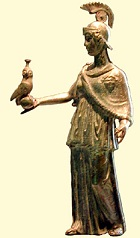
\includegraphics[scale=.9]{a20110630TheOwlofMinerva-img001.jpg} 
\end{wrapfigure}

This proverb from Hegel means that philosophy can only understand a cycle at its end. Hence, it is not helpful at its beginning, so anyone who is now engaged in the “battle of ideas” can hope for little more than a pyrrhic victory at best. Rather, it is a struggle of visions or world views. Pace Hegel, the Owl of Minerva is not a philosopher. The owl is wise not because he can think but rather because he can see in the darkness. While the world sleeps, the owl is vigilant at night. Thus, the men of Tradition must also be vigilant during the darkness.


At the beginning of a cycle, there is no need for philosophy. Man lives in immediacy following his Tradition faithfully and there is no need for questioning, and no need for wonder which is the motivation for philosophy. Unperturbed by the conflicts of competing thoughts, he lived with certainty. When an issue arose, he didn't think about it. Rather he followed the Tradition of his ancestors and his gods without question. His moral code was duty to the city, family, and gods. This code prescribed all his actions, which had to be executed precisely, and there was no room for subtleties. These rites maintained the souls of his ancestors and brought their blessings; he expected his sons to do the same for him after his death. These civilizations lived in relative internal harmony, sometimes for millennia.

Only with the decline of a cycle does thought arise. The corrosive effect of discursive thought calls everything into question. It no longer suffices to follow the ancestors and gods, one must also give a reason for doing so. Those skilled at logical and creative thinking become the philosophers. They offer their services to men in search of understanding. Others, such as the Sophists, notice that thought is an end in itself and can be used for persuasion apart from its actual truth value. The Sophists are the first propagandists and sell their services.

\paragraph{Three Civilizations}
\begin{quotex}
…bisogna tener ben fermo questo punto, indispensabile per una formulazione imperiale e romana dell'idea razzista e confermato da ciò che fu proprio alle grandi civiltà arie d'Oriente, all'antica Roma, al Medioevo romano-germanico.

\end{quotex}
We are focusing on the civilizations of the Borean race, as Fabre d'Olivet called it, who origins were in the mythical Hyperborea, whence it spread to India, Central Asia and Europe. There is not the time or energy to deal with the traditions of Asia, Africa, or the Amerindians. Furthermore, we have been focusing on just three Borean civilizations of a traditional nature, omitting the Nordic and Celtic traditions which are no less important. But since Julius Evola identified them as the three main civilizations of Indo-Eurpean origin, they serve as a good basis for discussion.

\begin{description}
\item[Hyperborea ]

We can get a glimpse into these people only through extrapolation. By the interpretation of myths we can try to reconstruct their society. For this, we are relying on \textbf{Bal Tilak}, \textbf{Fabre d'Olivet} and \textbf{Herman Wirth}. 

\item[Bharat Khant ]

Bharat Khant was the ancient name for the Vedic civilization of India. This is the oldest group that we have documentation for, which includes the Vedas and the Laws of Manu. It is most important for us today because of its rich metaphysical tradition which comprise the six orthodox schools, all deriving from the Vedas. This should not uncritically be confounded with the contemporary religion of Hinduism. Unlike Hinduism, the Vedic civilization included ancestor worship, animal sacrifice and rejection of reincarnation. 

\item[The Ancient City ]

By this, we mean the ancient city-states of Greece and Italy. Although their origins are obscure, their traditions and eventual decline are reasonably well documented. That makes their study invaluable to those of use seeking the light hidden by the darkness. 

\item[Christendom ]

Instead of circumlocutions such as “Medieval period” and the like, we will use this term to describe the civilization that arose in Europe following the fall of Rome, without intending by that term to impose a particular theological interpretation on it. To put a time frame on it, we mean the approximate thousand year reign from Constantine to the Reformation, which united spiritually much of Europe. We will see that it had its declines that mimicked the decline of the Ancient City, at least in principle if not in detail. But here we have the added advantage that its origins are also documented. Thus, we can see what it adapted from its predecessor and what it rejected. This will serve as a useful model for a new cycle. 

\end{description}
\paragraph{Three Types of Men}
Each period was marked by a special type of man who embodied its superior aspects. These were never theoretical men, or those with the “best idea”, but men of a higher knowledge, a direct knowing or gnosis that can never be fully encompassed in thought. The knowing took various forms.

\begin{description}
\item[The Seer ]

The type of the Vedic period was the \textbf{Rishi} and the \textbf{Yogi}. The Rishi, or seer, had clairvoyant vision to see into the nature or essence of things beyond the accidental, incidental, or the trivial. The Yogi was the man of power: for bhakti yoga, power over the emotions; for karma yoga, power over one's actions; for jnana yoga, power over one's mind. The jnani, or knower, was master of his mind. By transcending the stream of thoughts, which held no more significance to him than the movement of clouds across the sky, the jnani gained direct insight into the nature of things. 

\item[The Hero ]

The Hero of the Ancient City was the \textbf{Hero}, the patriarch of a family, the founder of the city. As priest, he was the link between the gods and men and had the power to invoke their blessings. As king, he had the power of command over men. He had the power to interpret the omens, because in order to predict the future, he had to create the future. 

\item[The Believer ]

Christendom began where the Ancient City left off, in particular, it separated the roles of priest and king, without, however, secularizing the latter as had been done in the successive revolutions of the previous era. This leads to two different figures, united in faith, although different in temperament. These are the Saint and the Knight. Rather than seeking godhood by means of the rituals and sacrifices of their sons as in the age of heroes, they relied on their respective devotions to the True God and the True Man. The \textbf{Saint} through his ascetical practices was drawn toward theosis (divinization). The \textbf{Knight} of heroic valor followed the path of the Fedeli d'Amore to lead to the alchemical marriage. 

\end{description}
\paragraph{The Way Forward}
\begin{quotex}
Io ho difeso e difendo idee … nella misura in cui riprendono una tradizione superiore e anteriore … in quanto appartengono al retaggio della carattere universale e mantenutasi in Europa fino all Rivoluzione francese. Nello stesso spirito … dei grandi filosofi cattolici del principio di autorità, de Maistre e Donoso Cortes … I miei principi sono solo quelli che prima della Rivoluzione francese ogni persona ben nata considerava sani e normali.

\end{quotex}
The way forward is indicated by Evola as quoted above: to defend the higher traditions of Europe that every well born person considered sane and normal. We need not look back to the distant past, just to Europe before 1789 since these principles have a universal character. To reject these principles, as those of the new right seem to do, is to squander our legacy and dishonor our ancestors. If anyone is unclear about those principles, please read Donoso Cortes’ essays\footnote{\url{https://www.gornahoor.net/library/CortesEssays.pdf}}, as Evola recommends.

The way forward is based on authority as illustrated by our examples. In future posts we will lay out some programs described by \textbf{Fabre d'Olivet} and \textbf{Saint-Yves d'Alveydre} based on theocracy, Synarchy and the spiritual unity of Europe. But ultimately, it will depend on men of vision, seers, heroes, and those of unshakable faith.

\flrightit{Posted on 2011-06-30 by Cologero}
\section{The New Intellectual}

\begin{quotex}
\emph{Noli foras ire, in te ipsum redi: in interiore hominis habitat veritas.}

Don't go outside yourself, turn back into yourself; the truth resides in the interior of man.

\flright{\textsc{St. Augustine}}

\end{quotex}
The following passage is taken from \textbf{Ultima Thule} by Arthur Branwen\footnote{\url{https://gornahoor.net/library/UltimaThule.pdf}}, where he is describing the beginning of Evola's interest in prehistory. [My translation.] 

\begin{quotex}
The central idea of this Evolian study, that along with other of his writing of that time shows the guiding influences of a new cultural perspective different from this earlier interests, was that in Germany of those years, there was emerging a type of culture intended to promote a spiritual and political rebirth that takes as its starting point the study of the most archaic roots of the German, and European, people. A culture that does not stop at pure erudition and tends instead to create a forma mentis, a reflection of a new state of mind tending to abandon the Spenglerian \emph{Decline of the West}, not assimilable in any way to the various sciences of antiquity studied in an ``antiseptic" manner in the universities which, on the other hand, in themselves do not demand any interior change and do not change in any way the relationship between man and the world. 

\end{quotex}
In other words, one cannot hope to understand these ancient myths without oneself becoming spiritually like the people who created those myths. One has to know the way they thought and felt, that is, their forma mentis. Man cannot be studied from the outside as though he is nothing but a chemical reaction.



\flrightit{Posted on 2010-06-30 by Aeneas }

\begin{center}* * *\end{center}

\begin{footnotesize}\begin{sffamily}



\texttt{Robman on 2010-07-01 at 10:21 said: }

This nordicist stuff just seems like the flip side of afro-centrism.


\hfill

\texttt{Cologero on 2010-07-01 at 12:15 said: }

I have no idea what afro-centrism is, nor what its ``flip side" is. Doesn't sound like much of an argument.

Bear in mind, we are not here defending any particular position. Just describing the theories and motivations for them from a particular era.

Nevertheless, we do accept the idea of a Primordial Tradition, so it is a legitimate question to discern its nature and origins. Wirth and Evola used myths, sagas, legends to try to answer that question. So, it is really the methodology we are dealing with, and its suitability for the subject matter — not a particular conclusion.


\hfill

\texttt{Robman on 2010-07-01 at 12:46 said: }

``Flip side" means reversal of, and afro-centrism is an movement by black ``scholars" in America who claim that blacks were the font of all culture, religion, and civilization. This ``primordial tradition" traditionalists like Guenon and Evola are fond of seems to be based on the argument there is a single metaphysic, and somehow they postulate that it must also have originated terrestrially in one place and then been dispersed through migrations. I don't believe the preponderance of historical and archaeological evidence bears this out, but of course then the counter-argument would be that that's because I'm a positivist rationalist who is limited in his scope. Yet I don't think the tenuous symbolism and legends the traditionalists use to buttress their argument are persuasive or point to any metaphysically super sophisticated nordic culture at the north pole either.


\hfill

\texttt{Matt on 2010-07-01 at 15:36 said: }

Robman,

Keep in mind that a significant amount of what Guenon and Evola talk about in their writings on the primordial tradition is meta-history. To them, the metaphysics that you speak of did not have a terrestrial origin. 

And although I'm not sure about Guenon, but Evola never believed all the human races and civilizations have a single origin (though if a lot of that is incorrect due to mistranslation of Italian or lack thereof, Cologero should not feel wrong to make the correction if I have made a mistake). He postulated that the indo-europeans and a few other races have a common origin (whether of a physical or non-physical nature), but they don't share a common origin with what he referred to as the southern races. From what it appears to me, Afro-centrists believe all races and civilizations have the same origin in the African race.


\hfill

\texttt{Robman on 2010-07-01 at 16:51 said: }

Matt, 

It seems to me that while they argue that the metaphysic is of a transcendent super-human order, if was nordic polar inhabitants who first gleaned it and then disseminated it south during their migrations. Otherwise, why else would Evola have been influenced by Wirth and decided that the primordial tradition was ultimately Nordic as opposed to mediterranean? Their view seems to have something of the hermetic ``as above, so below", insofar as terrestrial history should reflect meta-history.

But even if it is as you say it is, only a meta-history, then what is it we have here? Just another creation myth of a religious character?

As to human origins, they never seem to have clarified this point that I'm aware of. I know they reject evolution and hold that everything has devolved from a primordial golden age, including man himself, but what does this mean? How did man come to be then? Did he materialize into human biological form from spirit as theosophists claim?


\hfill

\texttt{Cologero on 2010-07-01 at 18:53 said: }

If you deny a single metaphysic, then you deny the possibility of knowing. The ``flip side" of positivist rationalism is that there is no possibility of knowing the truth; just a never-ending series of scientific postulates always in danger of being overthrown. As to the question of origins, science has shown itself to be noticeably inept, in particular, of explaining the origin of the universe, life, and thought. Yet we experience the world around us, our life, and our thinking. You can leave the question there, in the vain expectation that a future scientist will explain it all someday. Or you could be, like a very small group of men, driven to discover a more incisive methodology that can lead to an understanding of the answers to such questions.

So it is not unfair to claim that the positivist rationalist is limited in his scope, since he himself denies the possibility of transcending that limit, whereas the metaphysician does not. It's your life and your choice (assuming you accept the possibility of ``choice"). Live it the way you prefer.


\hfill

\texttt{Cologero on 2010-07-01 at 18:56 said: }

Yes, leaving out the details, that is more of less Evola's position. There is a book published about 100 years ago by an educated Hindu titled, ``The Arctic Home of the Vedas", which brought much evidence to the same thesis. It has not been disproven, as much as neglected, since such a view is now regarded as ``politically incorrect".


\hfill

\texttt{Cologero on 2010-07-01 at 19:06 said: }

As the article pointed out, the questions you ask cannot be answered in a satisfactory way to a positivist rationalist; it requires a change of consciousness. As a starting point, ask yourself the following questions:

1) How did you come into existence? Not just as a body, but as ``Robman" with a sense of identify and will.

2) When did you first become aware of yourself as an ``I", a separate being from your social milieu.

3) How do you accomplish anything? For example, dinner tonight. Did you plan it, think about it, envision it? Then did you act on it, perhaps by shopping, cooking, or eating out? How exactly does an idea in your mind — or spirit, English hides the equivalence of the two words — materialize itself into physical form?


\hfill

\texttt{Will on 2010-07-01 at 19:12 said: }

Part of the importance of myth is its function as `neuro-linguistic programming.' As Cologero wrote, ``one cannot hope to understand these ancient myths without oneself becoming spiritually like the people who created those myths."

To some extent, whether or not a myth is literally or historically true is of secondary importance. Or rather, the literal is only one level of meaning in myth, and a rather superficial one at that. When we are young, we believe the stories about heroes and gods to be literally true. Then we get older and more skeptical, and we doubt that these things could have actually happened. But if we persist in engaging myth, deeper levels of meaning begin to open up, such as the principles or ideals that myths can express.

So I'm not particularly concerned with whether or not human beings came from the North, or from Africa. Each is a myth that serves a particular function for particular people. I think Robman's observation about Afrocentrism and Nordicism has some truth to it. But I don't think this poses a problem. I sympathize with Afrocentrism to the degree that it can create ennobling myths for people of African descent. All peoples benefit from such myths – it gives you something to live up to.

These days, we're all supposed to believe that we are the chance mutations of monkeys. That's not very ennobling. Indeed, it tends to give people license to give in to their lesser natures – after all, we're just mammals with `selfish genes.' Maybe in the future human beings will figure out a way to make this mythos work for us. But as for now, we seem to be stuck in the ``world where God is dead" that Nietzsche and Evola wrote about.


\hfill

\texttt{Cologero on 2010-07-01 at 22:08 said: }

You cannot compare the \emph{use }of myth to come to a spiritual understanding with the artificial creation of a myth, or better said, ``noble lie"; they are of a totally different and incomparable order.

The fundamental reason, as we have endeavored to make crystal clear, is that this spiritual understanding is available only to the few; in particular, only for those few willing to undergo the spiritual transformation necessary for such an understanding. This is quite different from ``noble lies" intended to influence the masses.


\hfill

\texttt{Will on 2010-07-01 at 22:56 said: }

There is a story from the Buddhist tradition in which a man is traveling to India. His mother, a very devout Buddhist, learns of this and makes her son promise to bring her back some sort of relic or holy object from the land of the Buddha's birth. The son promises, but in the course of his travels, forgets to get anything. So on the way back, he sees the corpse of a dog laying in the street, and he pulls a tooth from it. He tells his mother that he has brought her one of the teeth of the Buddha. She believes him and venerates the tooth as a sacred object. Through her faith and devotion, she generates real merit and ultimately becomes enlightened.

In this story, the distinction between a noble lie and an authentic myth is blurred. It suggests that what one brings to one's spiritual practice – one's general disposition and intention – is, if not the most important factor, then at least a very important one.

This is not to say that we cannot distinguish between authentic, traditional myths and modern counterfeits (like that book The Shack, for example). But I think we have to keep in mind that what works for one person will not necessarily work for another.

This relates to Burckhardt's exposition of the relation between knowledge and will. If one is fortunate enough to encounter good doctrine, including good myths, then presumably this can expedite one's spiritual growth. But if one is not so fortunate, and is born into some strange cult or without access to good teachers, one can still progress if one's intention is pure.

I have to take issue with your statement that spiritual understanding is available only to a few. While I certainly agree that only a few achieve profound realization, all traditional doctrines state that what is realized is in fact common to all. Even Evola acknowledged this, and they don't come much more anti-egalitarian than him.


\hfill

\texttt{Robman on 2010-07-02 at 01:33 said: }

Having to choose between a potentially spiritually transforming ``noble lie" and the existential quandary rationalism leaves one in is an unsettling one to have to make, but personally, it would probably be my nature to choose the latter. I'm asking myself what would be the purpose of traditional metaphysics? For one to reintegrate himself with metaphysical reality? If so, how does a ``noble lie" of a nordic polar realm, if it were only a fiction, help achieve this transformation?


\hfill

\texttt{Will on 2010-07-02 at 10:28 said: }

Robman, I appreciate your question and your perspective. In my opinion, rationalism and ``noble lies" relate to what the Buddhist tradition calls nihilism and eternalism – the two extremes. Nihilism says that nothing means anything and we can't know anything, and eternalism vests everything with some kind of grand meaning. The right view is said to be neither of these.

Corresponding to these are extreme skepticism on the one hand, and extreme naivete or gullibility on the other. If we veer too far in either direction, our view becomes skewed. I've met plenty of new agers who are willing to believe anything that sounds vaguely `spiritual,' so long as it makes them feel good in the moment. That would be naivete. I've also met skeptical, `scientific' people who refuse to consider anything at all beyond a reductionist, materialist worldview.

The notion of a Nordic polar realm is related to the myth of the Golden Age. The Tibetans believe that the Kingdom of Shambhala exists either on this earth in a `hidden land' or in another dimension. Christians believe that the Garden of Eden still exists, but entrance is barred. I think these myths convey the notion that the divine is real and knowable and realizable, but I'm not entirely sure how important it is to `believe' in such things, particularly if one is more skeptically inclined. Perhaps other writers will have more to say on that. There are styles of meditation and practice that work with skepticism and the analytical qualities of the mind, such as the Madyamaka tradition in Buddhism. (That's the tradition I've studied the most, so sorry if my examples keep coming from there.) I think this relates to the earlier distinction between different types of yoga: jnana yoga (knowledge), bhakti yoga (devotion), etc. People have different inclinations and talents.


\hfill

\texttt{Cologero on 2010-07-02 at 12:51 said: }

Evola writes in Pagan Imperialism\footnote{\url{http://www.gornahoor.net/PaganImperialism/ThoseWhoKnow.htm}}:

\begin{quotex}
We, on the contrary—basing ourselves on a tradition much more ancient and real than the one which can be claimed by the ``faith" of Western man, on a tradition which is not proved by doctrines, but by deeds and works of power and clairvoyance—affirm instead the possibility and the concrete reality of what we have called ``Wisdom". We thus assert the possibility of a positive, direct, methodical, empirical knowledge in the ``metaphysical" field, just as the one science strives to gain in the physical field, and, just like science, it remains above any moral or philosophical belief of men. 

\end{quotex}
So you need not surrender your hard-headed rationalism, nor believe in any doctrines, myths, or ``noble lies". However, you do need the tools to investigate the metaphysical field, through direct and empirical experience.


\hfill

\texttt{Cologero on 2010-07-02 at 12:54 said: }

Thanks for posting this. We are definitely not talking about myths, allegories, or ``noble lies". The answer to the question of origins involves a knowing, not a believing.


\hfill

\texttt{Will on 2010-07-02 at 14:12 said: }

Thanks, everyone. I'm grateful to be able to discuss this with intelligent and civil people.

Gottling, that quote from Charles Upton is great, and also gives me some insight into Plato's doctrine of the Forms or Ideas, which I'm still trying to wrap my head around. Upton has a book on romantic love, which I haven't read yet, but I suspect it would inform the earlier discussion on chivalry and Tantra.

And the quote from Evola brings us back to the fact that what we are talking about is the potential to effect qualitative changes in our state of being. I'm curious to know what people think or have experienced about how this works. Does it relate to the feeling of inspiration and a kind of natural connection one has with certain ideas or myths? Since this discussion began with a question about Hyperborea, how might that myth or idea work in relation to gnosis?

Also, as an aside to Cologero, do you plan on finishing the translation of Pagan Imperialism?


\hfill

\texttt{Robman on 2010-07-02 at 14:50 said: }

Will, I don't mind the Buddhist references, since I too have somewhat studied it in the past decade and meditate regularly. My degree of ``enlightenment" is quite another matter, though. Buddhism as it is interpreted today is also another story altogether. I think it was Coomaraswamy who stated that Buddhism today is known for all the things it originally wasn't. Evola's book ``The Doctrine of Awakening" delves into pre-sectarian original Buddhism along those lines.

As far as the Nordic polar mythos, I'm not sure how it can be spiritually useful, except to a select few. This mythos, to my understanding anyway, seems to be directed at raising the spiritual esteem of those of Nordic or ``Aryan" racial type. I think Evola's idea was that spiritual race ultimately manifests in biological race, and that the Aryan type, as the highest caste, was some kind of spiritual elect. Though this idea is flattering if you're white, doesn't it ultimately fetishize race? Doesn't the Polar mythos foster the notion that metaphysical insight is the preserve of a select few? In this, it would become something akin to Judaism. And doesn't this ultimately lead to a biological attachment which hinders detachment and spiritual advancement?


\hfill

\texttt{Robman on 2010-07-02 at 15:03 said: }

Gottling, that was a difficult quote you provided and I'm not sure I understood it fully. However, I have read Upton's Atlantis and Hyperborea essay, and my reading of it was that Upton doesn't at all take it literally but merely symbolically.

Cologero, I read the words, and yet I have no idea what they really mean. Whether people speak of wisdom, metaphysical insight, experience of the noumen, gnosis, enlightenment, satori, mystical union, etc., to me it ultimately remains an abstraction. I haven't the foggiest what this experience entails, what it's aims are, or what imaginary polar nordic realms have to do with it. Even meditation for me is nothing more than a few stolen moments of psychological peace- far from any direct experience of niravana or the void, whatever that even means. Maybe I am just a profane modern westerner, but that's where it stands.


\hfill

\texttt{Matt on 2010-07-02 at 18:10 said: }

Robman,

Evola's quote is speaking about the way knowledge of the metaphysical/transcendent is obtained. Evola explains that its not obtained from mere faith that modern western Christianity preaches, nor can it be obtained from the rational discursive thinking. It can only be obtained by a direct experience. Evola has described it as a type of positivism (or spiritual science), a higher positivism, similar in a way to the lower positivism of the physical sciences that obtain knowledge (though be it of a relative nature) of the physical dimension from a direct empirical way. And since Evola sees the way to knowledge of the metaphysical as a science, it is therefore beyond typical moral trappings. This is the method of the long past western initiatic tradition, and to a lesser extent seen in the Eastern Orthodox doctrine of theoria that teaches a direct empirical experience of God's uncreated energies, which is the only concrete way of knowing the divine (unlike Catholicism's idea that only faith and/or rational discursive thinking are the ways to know the divine, or the protestant idea that the divine can only be known from naive faith). And for Evola, only the few have the ability to successfully follow this way, and the modern age makes it that much harder for western man since the initiatic tradition has been almost entirely lost in the west.

And Will, I share the same sentiments. Its nice to talk about these ideas in a civil manner, which is rarely seen today, especially on the internet. It reminds of one of Cologero's earlier posts on the respect shared between certain thinkers of the western tradition, who had a respect for each other even if they disagreed notably in some areas. Unlike most men, they did not view ideas as weapons to be used against each other.


\hfill

\texttt{Will on 2010-07-02 at 20:57 said: }

Robman, I agree with your comment about the fetishization of race. I am not happy about the co-optation of Traditionalism by people whose main agenda is identitarian politics. According to traditional doctrine, the only identity that ultimately matters is the Atman, or tathagatagharba, or God. This is not to say that racial and cultural traditions don't matter at all, but if we are going to discuss them in light of Tradition, I think we should keep our priorities in line. Otherwise, the kind of biologic and egoic attachment you mention comes into play. Fortunately, the `negative theology' of the Buddhadharma, which ruthlessly analyzes all phenomena as impermanent and not-the-Self, is a good antidote to such thinking. NA ME SO ATTA!

That being said, I do find the Polar mythos interesting, and I certainly don't care that it isn't politically correct. Nowadays, there is a tendency to view these types of studies through the lens of Nazism, as if that was somehow the only possible outcome of such a line of thought. But to dismiss a whole generation's scholarly and philosophical work because of some notion of guilt by association is really throwing out the baby with the bathwater. It's wrong to attach a stigma to Germanic myth and ancient history just because the Nazis liked it. 

Evola has a great line in Men Among the Ruins: ``The Idea, only the Idea must be our true homeland. It is not being born in the same country, speaking the same language or belonging to the same racial stock that matters; rather, sharing the same Idea must be the factor that unites us and differentiates us from everybody else." Personally, this is the view I subscribe to. I am most impressed by people who display admirable qualities such as wisdom, skill, strength, self-control, modesty, determination, perseverance, and other such virtues.


\hfill

\texttt{Will on 2010-07-02 at 21:11 said: }

Matt, I like your exposition of the Evola quote. The notion of ``higher positivism" seems to me an apt description of what that first and greatest generation of Traditionalist writers were doing when they ingeniously laid out the objective metaphysical unity behind the seemingly disparate religious traditions of the world.

In regards to Evola's views on methods – how to go about actually striving for this direct knowledge that can manifest ``deeds and works of power and clairvoyance" – he seems to have focused most on that in Introduction to Magic. And as you said, magic for Evola is a science – a `science of the I."


\hfill

\texttt{Robman on 2010-07-02 at 21:57 said: }

I don't care about the political incorrectness of the polar myth either, and that's not why I question it. I'm just curious as to its veracity and the coherence of traditionalist claims- whether it is historically true, or if it's only archetypal symbolism.

As to Evola, I get mixed signals from reading the man. On the one hand, he emphasizes the idea as you note above, yet at the same time seemed to stress Aryanism as the highest of karmic human destinies within manifestation, not just as a caste and spiritual type, but as a corresponding physical type as well. In one of his books, which I don't believe has been translated into English yet, he delves into physical anthropology and provides numerous pictures of European types with his own typological classifications. Which is it?

As far as his race of the spirit and line about ``The Idea", this sounds eerily like what modern liberals are trying to construct in modern ``proposition nation" America. The results, in my opinion, are negative. So again, Evola often confuses me.


\hfill

\texttt{Robman on 2010-07-02 at 22:19 said: }

Since we've been discussing Herman Wirth and Hyperborea, here is an article you might or might not find somewhat interesting. 

\url{http://heatherpringle.wordpress.com/2010/02/23/herman-wirth-and-the-origins-of-writing/}

It seems this work might back up some of Wirth's ideas. But what is especially striking to me is where it states:

``Indeed, she proposes that the ancient sign language may have originated in Africa and arrived in Europe with modern humans–a proposal that would have horrified Wirth."

I can't imagine that Chinese, or Africans, or Central Americans, or anybody else, for that matter, would be so generous and anxious to ascribe cultural developments found on their own soil to Europeans, for example. Yet western scholars often seem so frivolous with the western legacy in letting others take credit for it. The vast bulk of modern westerners do indeed seem to fetishize race, but other people's races rather than their own. What strange people we are.


\hfill

\texttt{Will on 2010-07-02 at 23:23 said: }

The observation about the similarity to the `proposition nation' concept is good. Realistically, I don't think you can make a nation that way; certainly not one as large as the United States. But a tribe or an organization or small community, perhaps.

Also keep in mind Evola's notion of the two ways of being outside the caste system: as a transcender, or as a pariah. In his call for an elite based on spiritual vision and principle, he is calling for transcendence of the caste system, whereas the liberal notion of the `proposition nation' seems to be more about the lowest common denominator.

I can't comment on the Evola text that you mention as I haven't read it. I can only say that I don't regard him as an infallible source, although obviously I respect his work a great deal. In his autobiography, he describes his work on racism as an attempt to introduce superior, spiritual principles into the discussion, which was widespread at the time, and which was overrun with the biological reductionism that he considered an error. I think Evola saw the Aryan idea as a suitable Ideal for the West, but in his writings it's clear that he respected the accomplishments of many cultures – not in a modern, PC relativistic way, but based on merit and objective evaluation. I'd like to see more of that. In modern politics, it seems like you have to choose between being a relativist or a chauvinist.


\hfill

\texttt{Robman on 2010-07-03 at 12:02 said: }

Will, here is the text I was referring to, but it's in German, and though my German is limited, I was able to glean the gist of some of the captions below the pictures provided. But it does look like Evola was delving into physical typology here:

\url{http://www.velesova-sloboda.org/misc/evola-grundrisse-der-faschistischen-rassenlehre.html}

For example, if you look at plate no. 8 of Buddha, Evola writes, ``classical Nordic Aryan features are visible".


\hfill

\texttt{Will on 2010-07-03 at 23:06 said: }

Robman, thanks for the link. I don't read German, so I'm afraid I'm still at a loss here. I did look at the pictures, but without being able to read the commentary, I don't know in what context they are being displayed.

A couple thoughts come to mind on this.

In regards to the picture of the Buddhist statue (it doesn't look like Saykamuni – maybe Padmasambhava?) the tradition holds that there are certain `marks' of a Buddha; among these, many physical characteristics. I don't have a list of them offhand, but these characteristics provide guidelines for artists in the tradition when they are depicting Buddhas in their artwork. The long earlobes are one such mark.

Within the Buddhist tradition, the three aspects of being – dharmakaya, sambogakaya, and nirmanakaya; or essence, energy, and form – are considered inseparable, and so it follows that the outer form would have some relation to the spiritual essence of a person.

So Evola may have held, in accordance with traditional doctrine, that certain physical characteristics correspond to certain psychological or spiritual traits (Yukio Mishima has some similar ideas in his book Sun and Steel.) Or he may have been adapting his ideas to the already existent German discourse on race, in his attempt to influence the course of events there. I don't know. Interesting that the photos are all of faces, not whole bodies. Mishima wrote instead of bodily traits and their correspondences. Can one be obese and still be `Aryan?' (According to the Tibetans, yes: Dolpopa, the founder of the Shentong school, was so fat he had to be carried around on a door. He was also the most enlightened teacher of his time.)

I find it ironic that people today condemn Evola for his views on race, when the fact of the matter is that it took more guts for him to propound these views directly to Fascist and National Socialist authorities – views that were very `politically incorrect' according to the standards of the time – than it does to condemn him today. Indeed, anti-Semites at the time condemned Evola because they noted that, according to his doctrine, a Jew could have the soul of an Aryan, and vice versa, which makes it very difficult to persecute Jews!

As Socrates discovered, the rabble hates a man who makes them think.


\end{sffamily}\end{footnotesize}

\section{Archaeology of the Soul}

\begin{quotex}
What tradition can remain to us of those generations that have not left us a single written line? … Fortunately, the past never completely dies for man. Man may forget it, but he always preserves it within him. For, take him at any epoch, and he is the product, the epitome, of all the earlier epochs. Let him look into his own soul, and he can find and distinguish these different epochs by what each of them has left behind.

\flright{\textsc{Numa Denis Fustel de Coulanges}, The Ancient City}

\end{quotex}
What we see described here is a method to uncover tradition. Like an archeologist at a site, we dig deeper and deeper into the soul to uncover more and more layers. Mr. Fustel studies legends and rites preserved by later Romans in order to extrapolate backwards to more ancient times. He also makes connections to the Vedas and Laws of Manu, which have been preserved until our time. Mr. Fustel was neither an esoterist nor a Hermetist, yet he understood this method. How much more, then, can a Hermetist uncover in a similar manner.

A simple Internet search will display incessant arguments about whether or not such and such a writer (e.g., Aurobindo) is a ``traditionalist" or which ``tradition" is more suitable. These discussions are along the lines of which tattoo to buy; different tattoos may appeal to different types of men, yet it will never be more than skin deep. Gornahoor is not interested in such debates, since there is only one Tradition: call it the Hyperborean Tradition\footnote{See Section \ref{sec:HyperboreaPrimordial} in this book.}, or the Indo-European, or La Tradizione Romana\footnote{\url{https://gornahoor.net/?p=1275}}. The way to understand it is to return to the Primordial State, deep within the soul. Hermetists do not recognize each other through their erudition, but rather through their depth. 

Thus, Gornahoor wants to change the terms of the discussion. Whatever your exoteric path, your ``tattoo" as it were, there are some common elements. The Hermetist must undergo the three trials\footnote{\url{https://gornahoor.net/?p=1902}}. He must master the four elements\footnote{\url{https://gornahoor.net/?p=1161}}. He understands the cosmic and juridical order\footnote{\url{https://gornahoor.net/?p=2053}}. He practices Hermetic meditation\footnote{\url{https://gornahoor.net/?p=898}}. He must have drunk the silence\footnote{\url{https://gornahoor.net/?p=1082}}, by calming the oscillations of the mind\footnote{\url{https://www.meditationsonthetarot.com/moral-purification-of-the-will}}. He understands the esoteric meaning of power and his True Will\footnote{\url{https://gornahoor.net/?p=1993}}.

In short, this path is not for the man with a pedigree but rather for the Twice-born, or noble man\footnote{\url{https://gornahoor.net/?p=1216}}. This path is not for the man with a degree, but rather for the man of power\footnote{\url{https://gornahoor.net/?p=1856}}. This path is not for the specialist, but rather for the \textbf{genius}\footnote{\url{https://gornahoor.net/?p=319}}.



\flrightit{Posted on 2011-04-13 by Cologero }

\begin{center}* * *\end{center}

\begin{footnotesize}\begin{sffamily}

\texttt{HOO on 2011-04-14 at 13:01 said: }

`According to this second and new version of history, civilization breaks down into epochs and disconnected cycles. At a given moment and within a given race a specific conception of the world and of life is affirmed from which follows a specific system of truths, principles, understandings, and realizations. A civilization springs up, gradually reaches a culminating point, and then falls into darkness and, more often than not, disappears. A cycle has ended. Perhaps another will rise again some day, somewhere else. Perhaps it may even take up the concerns of preceding civilizations, but any connection between them will be strictly analogical. The transition from one cycle of civilization to another—one completely alien to the other—implies a jump, which in mathematics is called a discontinuity.' [Evola, J. ``The Hermetic Tradition" p. 13]


\hfill


\texttt{Cologero on 2011-04-15 at 07:59 said: }

Yes, Hoo, but you omitted the following paragraph, in which Evola continues with his own version of the archeology of the soul. Otherwise, there could be no possibility of recovering the Hermetic tradition, which may be latent in some of us, those of us who ``remember". Evola claimed that there still existed some Roman families who maintained a hearth and continued to practice the ancient rites.


\end{sffamily}\end{footnotesize}

\section{The Science of Prehistory}

In \emph{Il mito del sangue}, \textbf{Julius Evola} has an important chapter on the theories of \textbf{Hermann Wirth}. In particular, Evola is interested in Wirth's thesis of the Polar, or Hyperborean, origin of the Nordic race, a theory that himself accepts. He begins the discussion with a quote from Oswald Menghin, the rector of the University of Vienna: 

\begin{quotex}
More than any other discipline, the science of prehistory has been brought, and even more, should be brought, to the center of the spiritual battle of our times. I don't think I'm mistaken in asserting that general prehistory will be the science that guides the next generations. 

\end{quotex}
Unfortunately, Prof. Menghin's advice is little followed today. There are a few reasons for that. The primary reason is that few people are even aware that there is a spiritual battle in progress; moreover, even fewer, probably, even understand what a spiritual battle is. 

Then there is the problem of methodology. The belief is prevalent that the only approach involves the scientific method. Perhaps this method can provide a little information, but it does not, and never could, offer any insight into the inner nature or spirit of prehistory. Obviously, that would prove useless in a spiritual battle. 

Finally, there is the question of pragmatism. Because of the emphasis on the false doctrine of evolution, few see the purpose of even looking into the prehistorical past in order to gain insight into the present. In this view, it is the future that matters, and the past something to be overcome or forgotten. 

Yet, at the time he wrote, Evola had reason to be optimistic. He continues: 

\begin{quotex}
In recent times there can be found in many circles a significant impulse to return to origins. The origins, here, appear under a special, spiritual light. He turns back to a presentiment that in primordial times he lived in a still pure state with meanings and symbols that were then lost, obfuscated or altered. Prehistoric research was brought from the level of lifeless scientific-archeological or anthropological positivism to a level of spiritual synthesis, guaranteed, thereby, to open new horizons for the true history of civilization. 

\end{quotex}
This impulse apparently ran out of gas. Instead of opening new horizons, we have three major theories of origins that limit what we know about ourselves. 

The first is the biological view, that man is a genetic accident, made ``in the image of animals", or that the Nordic race evolved out of Africa. The individual is no longer a spiritual being with a Will, but rather the resultant of various electro-chemical processes in the brain. 

Next is the return to polytheism. First of all, the purpose of the study of prehistory is not to return to the forms of the past; they are ``the past" for a good reason. Secondly, as we learned from Guenon, polytheism is a sign of decadence and any genuine primordial tradition is necessarily monotheistic. 

The worst, of course, is the negative, whiny, and ignorant rants of some who see nothing but decadence and disease, not only in the present state of Western man, but also in the past. Instead of recognizing a primordial unity, they propose a plurality of unrelated peoples and ideas. Compare that with the grand and inspiring vision —\textit{The Flowering of European Civilization} of \textbf{Donoso Cortes}\footnote{See Section \ref{sec:FloweringEuropean} in this book.}—, that unifies the greatest civilization of the West and relates them to the present.



\flrightit{Posted on 2010-06-28 by Aeneas }

\begin{center}* * *\end{center}

\begin{footnotesize}\begin{sffamily}



\texttt{Cologero on 2010-07-02 at 12:57 said: }

It is important to recognize that the rejection of the ``theory of evolution" is not the same as believing in some sort of so-called ``creation science". The point is that science is simply not competent to deal with the topic; it necessarily remains in the realm of metaphysics. ``Involution" is a metaphysical concept.


\hfill

\texttt{James O'Meara on 2010-07-09 at 10:32 said: }

Re 5:

Yes, the issue isn't `evolution' at all the rather the mechanism of `natural selection’ [the `biologism' of point one above]. Evola was perfectly happy to speak of `evolution of the soul,' for example. The materialists have cleverly gotten everyone to use `evolution' to mean simply `change' which no one, of course, denies; except for some ``5,000 year" creationists. And that's the other clever move: to label anyone who questions `natural selection' as a knuckle-dragging Bible-thumper.


\hfill

\texttt{Cologero on 2010-07-12 at 12:40 said: }

Yes, though the complete statement of the theory is ``natural selection by random variation".

It is not so much the ``natural selection" part of the theory, since every organism must be able to survive in its environment. It is the ``random variation" — which is really a non-explanation — that is in question, since everything must have its sufficient reason.

As Evola and other Hermeticists say, the sufficient reason for existence is Will. That is the point of the True Will, to manifest one's highest possibilities. Manifestation (things that happen) seems random to those who sacrifice their will to external forces.


\end{sffamily}\end{footnotesize}

\section{Hope and Change}

\paragraph{Hope}
\begin{quotex}
Even the smallest initiative of a single man or group of men when it is properly organized, can result in a surprising variety of effects and long-term results. As soon as one realizes this fact, one becomes completely immune against despair. \flright{\textsc{Charles Maurras}}

\end{quotex}
\paragraph{Change}
\begin{quotex}
History sometimes produces surprising reversals or changes of direction. The secret of action consists in recognizing them and knowing how to make use of them, for although obviously we are not going to be able to reverse the whole direction of events by our personal and random tinkering with its works, sometimes quite a small push or twist of ours can set it rolling in a different direction and at a different speed. \flright{\textsc{Jean Ousset}, \emph{Action}}

\end{quotex}


\flrightit{Posted on 2011-07-04 by Cologero }


\chapter{Hyperborea}
\section{Hyperborea and the Primordial Tradition}

\begin{quotex}
In general, the men whom pride makes melancholy, always discontented with the present, always uncertain of the future, love to reflect upon the past from which they believe they have nothing to fear; they adorn it with smiling colours which their imagination dares not give to the future. They prefer, in their somber melancholy, superfluous regrets without fatigue to real desires which would cost them some efforts. \flright{\textsc{Fabre d'Olivet}}

\end{quotex}
\paragraph{Introduction}
There exists an egalitarianism of thought, whose presumption is that human consciousnesses are fundamentally alike, both across time and also across the different strata within society. But this is irreconcilable with some fundamental metaphysical principles\footnote{\url{https://www.gornahoor.net/?p=823}}: the doctrine of cosmic cycles presumes a difference over time (diachronic) and the doctrine of castes presumes a difference within time (synchronic).

Previous writers on Tradition have not always drawn out fully the consequences of these doctrines. Their view has been static and treated the various traditions as though they were mushrooms arising spontaneously after the rain. The consequence has been that ``tradition" often devolves to a type of comparative religion with debates about which tradition is the ``best" or more ``suitable", and so on, based on little more than contingent historical events or polemical ``sound bites". Instead, these doctrines should throw light on why certain forms appeared where and when they did and what is the relationship to each other. The Western or Roman Tradition is the evolution of the Hyperborean Primordial Tradition\footnote{\url{https://www.gornahoor.net/library/UltimaThule.pdf}} (understood as the unfolding in time due to the forces of cosmic cycles). Thus, we trace the development from the North to the East to the South and to the West. Then, towards the end of a complete cycle, the full effects of the Kali Yuga being to manifest. There are reasons for all this.

\paragraph{Diremption and Man}
The appearance of man brought about a diremption in the cosmos. This split Heaven from Earth, with Man as the reconciling force. Initially, the consciousness of man had direct intuitive knowledge of both Heaven and Earth; the soul, or psyche, was experienced as a life force or elan vital, rather than the complex of thoughts, feelings, likes, dislikes, images and so on, that trap man in subjective isolation.

\paragraph{Primordial State}
In contrast, the Hyperboreans in the Primordial State would have lived in purity (undivided mind and will) in the light of the sun followed with long nights interspersed with a dim light on the horizons where the sun is struggling to rise or set.

There is abundance to satisfy all needs, the Hyperborean knows when he is satiated. The mind is free of fear, worry, anxiety. Death is experienced, not as destruction, but rather as a transformation to a different state.

There is an intuitive awareness of God and the universal order by clairvoyant vision, just as we now recognize a tree or a mountain by direct experience. Thinking is regarded as another sense, along with sight, hearing, touch or taste. Discursive thought — of the ``yes" and the ``no", of the ``good" and the ``evil" — is not present. Instead, thoughts are experienced as voices from the celestial hierarchies (gods or angels) or communications from ancestors or as commands from rulers.

Knowledge is passed on by myths, symbols, and rites, in poetic forms.

Temporal power is exercised without force and obeyed willingly; the structure of society is held together by bonds of loyalty, family, and love. Commands are experienced, not as an imposition from the outside, but rather as the direct revelation of spiritual authority in one's own consciousness.


\hfill

Recommended reading

\begin{itemize}
\item Anonymous, \emph{Meditations on the Tarot} 
\item Antoine Fabre d'Olivet \emph{Hermeneutic Interpretation of the Origin of the Social State of Man} 
\item Arthur Branwen, \emph{Ultima Thule: Julius Evola e Herman Wirth} 
\item B G Tilak, \emph{The Arctic Home in the Vedas} 
\item Julian Jaynes, \emph{The Origin of Consciousness in the Breakdown of the Bicameral Mind} 
\item Rene Guenon, \emph{The Great Triad} 
\item Rudolf Steiner, \emph{Spiritual Beings in the Heavenly Bodies \& in the Kingdoms of Nature} 
\end{itemize}


\flrightit{Posted on 2011-01-09 by Cologero }

\begin{center}* * *\end{center}

\begin{footnotesize}\begin{sffamily}



\texttt{James O'Meara on 2011-01-09 at 21:36 said: }

``Previous writers on Tradition have not always drawn out fully the consequences of these doctrines. Their view has been static and treated the various traditions as though they were mushrooms arising spontaneously after the rain. … Instead, these doctrines should throw light on why certain forms appeared where and when they did and what is the relationship to each other."

Oddly enough, I was re-reading Revolt Against the Modern World this weekend, and it occurred to me that this is exactly what makes Evola distinctive. Part One constructs a model of ``Tradition" derived from a survey of world traditions, using a method of synthesis [``the Traditional Method"] which I've previously compared to such methods as [here] to Spengler's ``physiognomic tact" and [on my blog] Clive Bell's artistic sense. Part Two then surveys actual [well, according to him] historical developments, identifying various `cycles.' as Tradition interact, declines, recoups, etc. 

By contrast, Schuon is the anti-Evola, taking each tradition as a `mushroom' or a-synchronic whole [``The Christian", ``The Taoist" etc.]. H. Smith took this model and calcified it further, if possible, into a cookie-cutter eso/exo model for all world religions, taken as such with no analysis at all.

This is exactly what made Evola so interesting, both theoretically as well as in practice [his attempts to influence contemporary events], after coming from reading Guenon etc., who by contrast seem like armchair theorists. 

Schuon take everything today as given, and accounts for change or conflict by the all-purpose `divine adaption.' Evola, and even Guenon, are able to dig beneath the surface and explain, say, the Roman tradition as an ongoing reconquest of telluric influences by a Nordic cycle etc.


\hfill

\texttt{Mark on 2011-01-10 at 16:00 said: }

I will post here to comment on Kadambari's comment that Putin has declared Russia an Orthodox country. The reality is that the adoption of Christianity by the Northern peoples has caused a rupture in their spirit. Their pagan imagination has a tendency to want to go to deeper myths.

\url{http://onlinelibrary.wiley.com/doi/10.1111/j.1469-8129.2008.00329.x/abstract}

``ABSTRACT. As in all post-Soviet states, the Russian intelligentsia has been preoccupied with the construction of a new national identity since the beginning of the 1990s. Although the place of Orthodox religion in Russia is well documented, the subject of neo-paganism and its consequent assertion of an Aryan identity for Russians remains little known. Yet specialists observing the political and intellectual life of contemporary Russia have begun to notice that the development of references to `Slavic paganism' and to Russia's `Aryan' origin can be found in the public speeches of some politicians and intellectual figures. This article will attempt, in its first section, to depict the historical depth of these movements by examining the existence of neo-pagan and/or Aryan referents in Soviet culture, and focusing on how these discourses developed in different spheres of post-Soviet Russian society, such as those of religion, historiography, and politics."

\url{http://www.springerlink.com/content/j30056125185344h/}

Perun's revenge: Understanding theduxovnaja kul'tura

The one thing that it seems that Kadambari has not been able to appreciate is the fact that a Christian conscious and a ``Pagan" unconscious has affected the people of the North in a different way than the people of the South.

It has interested me as to why the synthesis of Paganism and Christianity has caused a rupturing in the person of the North to the point where if we take someone from Scandinavian descent, if they take their religion seriously, then they become either a fundamentalist Protestant or Asatru, whereas this does not arise as much in the Greek or Italian.


\hfill

\texttt{Cologero on 2011-01-10 at 18:47 said: }

That is an interesting point, Mark. I have a post in mind that explores that very topic, though I've delayed it because it is inconclusive. Perhaps, I'll post it anyway, after a little preparation.


\hfill


\end{sffamily}\end{footnotesize}

\section{Arctic Home in the Vedas}

\begin{quotex}
From the dead sun springs a daughter more beautiful than her sire, and mankind starts afresh from the life-raiser and his bride-Life. 

\end{quotex}

In which we briefly outline the idea of cosmic cycles, and illustrate them initially in the revelation of the originary Hyperborean source of the Vedas. This is then extended to Traditions following the Vedas. Finally, there is some speculation on the future course of the West. The foundation is the book \textit{The Arctic Home in the Vedas} by \textbf{Bal Tilak}.

\paragraph{Cosmic Cycles}
Since a more complete exposition can be found in Rene Guenon's writings, from whom these notes are taken, and elsewhere, we provide here just the most basic outline.

\textbf{Cycle}: represents the process of development of some state of manifestation

\textbf{Minor cycle}: one of the more or less restricted and specialized modalities of that state

Since the \textbf{Law of Correspondence} links all things in universal Existence, is necessarily and always a certain analogy, either among different cycles of the same order or among the principal cycles and their secondary divisions

\textbf{Kalpa}: total development of a world. One cannot speak literally about its duration so that duration has a purely symbolic value. Perhaps not in our world because time is one of its determining conditions.

\textbf{Manu}: there are 14 Manus, each ruling over a Manvantara. There are two septenary series. The first septenary is that of descent, or devolution, and includes ours. The second is ascent or evolution.

\textbf{Manvantaras}: cycles have a character that is both cosmic and historical, they concern terrestrial humanity, also linked to events occurring outside the history of humanity. There is a correlation between the cosmic and human orders. This means, for example, that events in the human realm correspond to events in the celestial spheres.

These relate to the 7 \textbf{svargas} and 7 \textbf{patalas} which represent states respectively higher and lower than the human state. By correspondence, these can be related to the 14 manus.

\begin{wrapfigure}{rt}{.3\textwidth}
 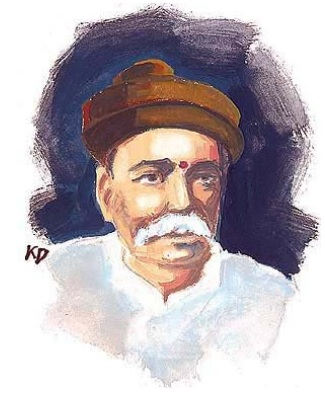
\includegraphics[scale=.5]{a20200723ArcticHomeintheVedas-img001.jpg} 
 \caption{Bal Tilak}
\end{wrapfigure} 

A Mantavara is subdivided into 4 \textbf{yugas}. We are allegedly in the last yuga, the Kali Yuga. The starting date and exact duration are not known, according to Rene Guenon.

There are 7 \textbf{Dvipas} or regions into which our world is divided. They are represented as islands or continents, but not parts of present-day earth. They may also refer to planetary spheres.

These ages, states, and regions also have symbolic meanings, since there is a sacred geography as well as a profane geography. Henry Corbin discusses this topic in his books, and it is also confirmed by Rene Guenon:

\begin{quotex}
There is also a symbolical geography; indeed, in this connection, there is a very significant correspondence between the domination of the West and the end of a cycle, for the West is the place where the sun sets. 

\end{quotex}
Thus, when he mentions the distinction between Eastern and Western understanding, this is no way simply a geographic distinction; i.e., there is no ``magic dirt" in the East. Guenon amplifies the idea:

\begin{quotex}
To the extent that a man `Westernizes' himself, whatever may be his race or country, to that extent he ceases to be an Easterner spiritually and intellectually. 

\end{quotex}
The converse is also true. Unfortunately, this is too often overlooked so there are some who fantasize about going east to find an ``initiatic centre" or give up entirely. Often, they justify this decision because of the ``corruption" they see in the Church hierarchy, as though India and Egypt are free of such corruption. These masters of ignorance have a loud presence on social media. The truth is that real initiates like Savonarola, Boccaccio, and Dante were complaining about corruption in the Church a thousand years ago. (See Canto XXI, \emph{Paradiso}, for example.)

How, then, could Dante describe his spiritual journey? His passage through Purgatory and Heaven are descriptions through the higher and lower stages. Guenon provides us with the general idea, but we need to get the details from others who have made the trip.

\paragraph{Hyperborean Migration}
The idea of a migration of a branch of the Borean race from a polar region to India has been a mainstay in esoteric literature. That is now considered outré and dismissed as the ``Aryan Invasion Theory". Times change. Bal Tilak, the author of The Arctic Home in the Vedas, was a Hindu nationalist and considered himself to be Aryan; so, it is not a Nazi fantasy. Perhaps there is no genetic, archaeological, or documentary proof. Nevertheless, as Georges Dumezil documented, there is still the trifunctional social organisation from Scandinavia, across Europe, to India that needs to be explained. Moreover, there is similarity in the mythologies of the various Indo-European people.

In any case, it may be best to regard Hyperborea as transcendent geography or one of the seven Dvipas. That is how the Greeks understood it, since only the gods could visit it. Apollo would arrive there by a swan.

Nevertheless, Tilak probes through the Vedas looking for clues for an actual migration several millennia ago. In particular, he sees astronomical facts that match the experience of a those living in a land close to the North Pole. For example, the original Roman calendar had 10 months, ending in December. That is because it would be followed by two months of darkness during which days could not be counted. It continues in that vein, relying as much on Western scholars as on the Vedas themselves.

Sometimes it gets tedious, much like exegesis on Genesis; is a ``day" 24 hours or does it refer to an age? Nevertheless, it is worth the trouble because of the vast amount of information in it.

The Vedas are eternal and without beginning. However, we owe the textual version to the seven Rishis who could ``see" the vedas from the beginning of the Kalpa. A deluge had destroyed the Vedas at the end of the previous Kalpa. Tilak's method is to juxtapose the Theological view in the Vedas with a corresponding Historico-scientific view gathered from external and profane sources. He also relies on comparative mythology relating Celtic, Greek, Roman, and Egyptian myths to corroborate the Vedic myths. Most importantly, Tilak regards the Zend Avesta, the sacred text of the Zoroastrians, as authoritative.

\paragraph{The Divine Word}
Since, this is an introduction, we can only point out some highlights; maybe someday we can do a more exhaustive review. This is an important point:

\begin{quotex}
Vedic names and forms of species are eternal, and it is by remembering these that the world is created by Brahmâ at the beginning of each Kalpa. The Veda is, therefore, the original WORD, the source from which everything else in the world emanated, and as such it cannot but be eternal. 

\end{quotex}
Tilak points out that this doctrine is tantamount to the notion of the divine \emph{Logos} of the Alexandrian school.

The duration of the various ages or yugas were in dispute. For example, by an early reckoning, the Kali Yuga would have ended soon after the birth of Christ. Although they knew nothing of that event, the authors of the Puranas in the first centuries AD, refused to believe the Kali Yuga had ended. Hence they extended the duration from 1000 human years to divine years (360 human years). Tilak points to similar artifices to fudge the dates for various purposes. The alternative is to assume that the Christian Era represented the end of the Kali Yuga and the beginning of an ascent.

The point is that the authors preferred to understand the ages by their qualities, not merely as the passage of quantitative time. Also, the original timeframes were much shorter than the fantastical extended duration of the ages that get passed around today.

\paragraph{Excursus on Method}
Tilak is very thorough, although the text points out the difficulty of fully understanding the Vedas in all cases. Both Evola and Guenon accepted Tilak's thesis; the latter actually thought very highly of Tilak. Guenon reveals some contradictions in his doctrines that require explanation. For example,

\begin{itemize}
\item Guenon claims Tilak was a non-Westernized Hindu. \textbf{FACT}: Tilak was quite familiar with European science, history, and mythology. Moreover, he had deep respect for the German Indologist, Max Müller. 
\item Guenon tediously rails against ``profane" science, history, philosophy, etc. \textbf{FACT}: Tilak relied heavily on those ``profane" fields of study to fortify his thesis. 
\item Guenon hates Vivekananda, but loves Tilak. \textbf{FACT}: Vivekananda was esteemed by not just Tilak, but even Hindus in India to this day. 
\end{itemize}
The point is that it is a mistake to disdain ``profane" scholarship when it might be helpful. By the Law of Correspondences, science and metaphysics should not be in conflict since they deal with different levels of existence. Guenon has done us a great service by his explanations of metaphysics and symbolism, by his deep comparisons of different traditions, and by expanding our understanding to include the full range of authentic human spirituality. There is no ``Guenonian doctrine" per se, since he is just rephrasing the doctrines of traditions that pre-existed him.

At the end of the day, Guenon does not judge Tradition; Tradition judges Guenon. That is lawful, not a negative judgment.

\paragraph{Traditional Forms}
It is one thing to mention the possibility of different stages/regions/states, etc., and quite another to fill in the details. That would perhaps require another Rishi, not for a new revelation, but rather for a deeper understanding. Tilak gives us some clues about how the different stages of Tradition might look.

The Letters to the Seven Churches in the Book of Revelation represent the seven stages of the development of Tradition. The following list represents Valentin Tomberg's understanding of the stages. This list is remarkably consistent with Tilak's exposition of the Vedas, with some speculation about the future.

\begin{enumerate}
\item \textbf{Ephesus}: The old Indian (Vedic) culture. This is primal revelation given to the Rishis in India. 
\item \textbf{Smyrna}: The old Persian (Zoroastrian) culture. The Zend Avesta also retained a memory of the Hyperborean revelation. 
\item \textbf{Pergamos}: The Chaldean-Egyptian (Hermetic) culture. This is based on the revelation of the Logos to the Alexandrian school. 
\item \textbf{Thyatira}: The Greco-Roman (pagan) culture. Although the Greeks retained some memory of Hyperborea, much came through Egypt. The Greeks had the same understanding of ``name and form" from Vedic metaphysics, despite the different emphases of Plato and Aristotle. 
\item \textbf{Sardis}: The Anglo-Germanic (Christian) culture. The Christian religion transformed Europe with a deeper revelation. Building on the Vedas and Hermetics, it understood the Logos as not just the creator, but also as equal to God as well as saviour and judge. Christianity got its philosophy from the Greeks and its Theology was enriched by the Alexandrian school as Vladimir Solovyov pointed out. 
\item \textbf{Philadelphia:} The Slavic-Russian (also Christian) culture. The Slavic nations should be the preservers of Tradition. We shall see how that plays out. 
\item \textbf{Laodicea:} The American, i.e. Western Hemisphere, (future) culture. North and South America will look quite different in the future. More cannot be said at this time. 
\end{enumerate}
There are three churches of the past, two of the present, and two of the future. But do not take the history and geography too literally, for they represent streams that are always active in us.



\flrightit{Posted on 2020-07-23 by Cologero }

\begin{center}* * *\end{center}

\begin{footnotesize}\begin{sffamily}



\texttt{Christopher on 2020-07-23 at 15:48 said: }

``Guenon tediously rails against ``profane" science, history, philosophy, etc. FACT: Tilak relied heavily on those ``profane" fields of study to fortify his thesis."

While I agree generally with the tediousness of Guénon in this regard, I don't believe it to be a contradiction. Guénon has, at various times, cited archaeological findings (his article on La triple enceinte druidique comes to mind) and defended the potential use of profane archaeology, even while criticizing its current usage. In his article on the Place de la tradition atlantéene dans le Manvantara (Le Voile d'Isis, August–September 1931), he wrote:

« On ne saurait être trop prudent quand il s'agit de civilisations entièrement disparues, et ce ne sont certes pas les tentatives de reconstitution auxquelles se livrent les archéologues profanes qui sont susceptibles d'.claircir la question ; mais il n'en est pas moins vrai que beaucoup de vestiges d'un passé oublié sortent de terre à notre époque, et ce ne peut être sans raison. Sans risquer la moindre prédiction sur ce qui pourra résulter de ces découvertes, dont ceux qui les font sont généralement incapables de soupçonner la portée possible, il faut certainement voir là un «signe des temps» : tout ne doit-il pas se retrouver à la fin du Manvantara, pour servir de point de départ à l'.laboration du cycle futur ? »

``One cannot be too cautious when dealing with civilizations that have completely disappeared, and it is certainly not the attempts at reconstitution made by profane archaeologists that are likely to shed light on the matter, but it is no less true that many vestiges of a forgotten past are coming out of the ground in our time, and this cannot be without reason. Without risking the slightest prediction about what may result from these discoveries, whose possible significance is generally not suspected by those who make these discoveries, we must certainly see this as a `sign of the times.' Should not everything be found at the end of the Manvantara, to serve as a starting point for the elaboration of the future cycle?"


\hfill

\texttt{Logres on 2020-08-05 at 23:20 said: }

``The alternative is to assume that the Christian Era represented the end of the Kali Yuga and the beginning of an ascent." Rudolf Steiner seems to have come to this conclusion, and much of what you review in Tilak resonates with what I've been able to glean there.

\url{https://martyrion.blogspot.com/2015/11/jesus-of-gospel-of-matthew.html}

\begin{quotex}
It is not only in man that a change has taken place; everything in Nature, everything on Earth, was also changed at the descent of man. It was therefore not enough for man simply to say: All this is maya, is illusion — let us raise ourselves to the spiritual world! We shall then certainly have changed ourselves, but not all that has become changed in the world around us.' So the Iranian did not say: `Around me is maya on every side — I will rise above this maya, will overcome it in myself, and so attain to spiritual worlds.' No, he said: `Man belongs to the world around him; he is but a part of it. Therefore if that which is divine in him, and which descended with him from spiritual heights, is to be changed, then not only man must be changed back again, but everything that surrounds him must also be changed back to what it was.' This feeling gave this people a special impulse to enter energetically into the task of transforming and changing the world. While the Indian said: `The world has changed, deteriorated; what we now behold is maya,' the people of the north said: `Certainly the world has come down, but we must so change it that it is made into something spiritual once more!'

\end{quotex}
The idea being, that by the very fact of the Fall, lower matter is redeemed by the presence of the ruined image of God, and is now ``involved". This translates into understanding ``struggles between cultures", although not entirely literally. For instance, Steiner cites the Turanian struggle here:

\begin{quotex}
The Turanians in the north toward Siberia, who had inherited a lower astral clairvoyance, had no desire to establish external civilization, and their passive disposition, influenced by many priests who practiced magic, led them frequently to occupy themselves with lower magic, and even black magic. To the south, the Iranians, with an inclination to influence the sense world by their human spiritual force, were working in a primitive way at the beginnings of civilization.

This is the great contrast between Iranians and Turanians. These facts are expressed in a beautiful myth: the legend of Djemjid. 

\end{quotex}
Thank you for the note on the Seven Churches, and indeed, the entire article.


\end{sffamily}\end{footnotesize}

\section{The Hyperborean Race and its Branches}

\begin{quotex}
This is Part 2 section 7 of \emph{Sintesi di dottrina della razza} by \textbf{Julius Evola} in which he discusses the Hyperborean race. The texts that he refers to are \emph{Revolt Against the Modern World} and \emph{The Myth of Blood}; the chapters in Revolt on the Hyperboreans should be read in conjunction with section.

From the corporeal perspective, this can be understood as a specific race of humans. From a spiritual perspective, it can be understood in terms of sacred geography. In the latter case, the Hyperboreans represent a race of people who lived in the light, i.e., in self-effulgent consciousness. Or both interpretations can coincide. 

\end{quotex}
The limit that can be given to our doctrine of the race regarding the exploration of its origins lies at the point when the Hyperborean race had to abandon the Arctic home in successive waves following different paths, because of the freezing that rendered it uninhabitable—it was already pointed out, in previous citations, justification for the idea that the Arctic region became completely ice bound only after a certain period: the memories of that home, preserved in the traditions of all peoples in the form of various myths where it always appears as a ``land of the sun", as an island continent of splendour, as the sacred ground of the God of light, and so on, were already, in this respect, rather eloquent.

Now, at the point of the beginnings of the prehistoric Hyperborean emigrations, the Hyperborean race could be considered, among all of them, the superior one, the super-race, the Olympic race reflecting in its extreme purity the very race of the spirit. By and large, it seems that all the other human stocks existing on the earth in that period, appeared either as ``races of nature", that is, animalistic races, or, as races that had become ``races of nature" through involutions of the preceding racial cycles. In fact, the traditional teachings speak of a civilization or of an Antarctic race that had already fallen into decline in the period of the first Hyperborean emigrations and colonisations, and whose Lemurian residues were represented by sizable groups of black and Malaysian races. Another racial stock, distinct both from the Hyperboreans and from the Antarctic-Lemurians, was that which originally occupied the Eurasian continent (the Finnish-Mongoloid race) as the yellow-brown race and, as the as red-brown race and also again the yellow-brown, occupied both a part of the Americas and Atlantic lands that are now extinct.

It would obviously be absurd to attempt a precise typology of these prehistoric races and of their primordial combinations in regards to exterior characteristics. We must refer to them only to prevent some misunderstandings and to be able to orient ourselves among the ethnic formations of the successive periods. Also, the investigation of skull fossils can tell us very little, both because race is not characterized just by the skull, not even the simple race of the body, because there are reasons to justifiably assert that, for some such races, fossil remains could not be preserved up until our time. The dolicephalous, or elongated skull, combined with a tall and slim figure, blonde hair, clear skin, blue eyes, is, as we noted, characteristic of the most recent descendants of the Nordic races who came directly down from the Arctic regions. But all that does not constitute the final word; even within the limits of the positive order, it is necessary to bring in considerations proper to the study of the race of the second level [race of the soul] in order to get our bearings.

In fact, we already said that the essential element for race is not given by simple corporeal and anthropological characteristics, but by the function and the meaning that they have in the whole of a given human type. Dolicephalous men with a tall and slender build are also found in fact among the black races, and a white coloration and almost blue eyes are found among the Ainu of the Far East and the Malaysian-Polynesian races, naturally having a totally different significance in such races. Nor must we think here only of anomalies or tricks of nature, in certain cases being able to treat of extinct somatic survivals in the proceeding types from races which, in their most remote zenithal period, were able to have similar characters to those which, in the period we are considering, were instead found concentrated in the Nordic-Hyperborean element and here accompanied, up to a relatively recent period, by the significance and by the corresponding inner races.

As to the emigration of the races of Hyperborean origin, having previously written about them in the books previously cited, we can limit ourselves to noting three principle currents. The first took the direction northwest to southeast reaching India and having as its final echoes the Indian race, indo-afghan and indo-brachimorphic in Peters' classification. In Europe, contrary to what you may believe, the traces of such grand currents are less visible or, at least, more confused, because they had a superposition of waves and therefore a composition of successive ethnic layers. In fact, after this current in the northwest-southeast direction (the transversal Nordic-Aryan current), a second current followed the direction West to East, in most of its branches through the routes of the Mediterranean, creating centres that sometimes should be considered even more ancient than those derived from the preceding transversal wave, because in this case it is not always about a forced emigration, but also of a colonization occurring before the destruction or the eventual uninhabitability of the original centres of the civilization of Hyperborean origins. We can call this second current, with the related trunk of races, Ario-Atlantic, or Nordic-Atlantic, or, finally, Atlantico-Occidental. In fact, it originates from an Atlantic land, in which it constituted a centre that, at its origin, was more or less an image of the Hyperborean centre. This land was destroyed by a catastrophe, whose memory likewise is found in the mythologized memory of the traditions of almost all peoples, and then after the waves of the colonizers a true emigration followed.

It is said that the land of Atlantis was familiar at its origin with a type of facsimile of the Hyperborean centre, because the data reaching our time lead us to think that a regression happened, both from the point of view of race and from the point of view of spirituality, in these Nordic stocks who had already ventured towards the south in the most ancient epoch. The mixing with the red-brown aborigines seems, in this regard, to have had a destructive and sizeable role, and if a precise record in Plato's story is not found, in which the union of the ``sons of the gods"—of the Hyperboreans—with the indigenous people was given the blame in the end, that recall what, in other recorded myths, are described as the ``fall" of the heavenly race—of the ``angels" or, again, the sons of the gods, \emph{ben elohim}—who mated, at a particular moment, with the daughters of men (of the inferior races), committing a contamination significantly likened to, by other texts, the sin of sodomy, carnal relations with animals.


\hfill

Further reading

From the positive, scientific perspective, see \emph{The Science of God} where the physicist Gerald Schroeder discusses the existence of pre-Adamic hominoids.

In \emph{The Psychology of Man's Possible Evolution}, Peter Ouspensky mentions the possibility of the existence of pre-Adamic hominoids.

Boris Mouravieff, who claims to be drawing on ancient Western traditions, accepts the existence of a pre-Adamic race in his \emph{Gnosis} trilogy.

The idea of the polar origins of the Hyperborean race was discussed in \emph{The Arctic Home in the Vedas} by \textbf{Bal Tilak} based on myths recorded in the Vedas.

For a recent theological and metaphysical discussion of the existence of humanoid animals, see \textit{Knowing Ape from Adam}\footnote{\url{http://edwardfeser.blogspot.com/2014/12/knowing-ape-from-adam.html}}.



\flrightit{Posted on 2015-03-01 by Aeneas }

\begin{center}* * *\end{center}

\begin{footnotesize}\begin{sffamily}



\texttt{John Bardis on 2011-03-26 at 22:12 said: }

In regard to the reference to Mouravieff and the pre-Adamics, this has to do with the idea that a human has three so-called centers: moving, emotional and intellectual (while animals lack the intellectual center). But, then, humans also have higher emotional and intellectual centers.

According to Mouravieff there are, basically, two species of humans: those with higher centers and those without higher centers. So someone without the higher centers would be an animal with an intellectual center–a very smart animal.

Those without higher centers live only one life, like animals, then they die. People with higher centers reincarnate.

Those without higher centers can be quite attractive physically, as tends to be the case generally with animals. After all what is more beautiful than a horse or a tiger or a hawk? And, in fact, these people without higher centers very often have blue eyes and blond hair, as everybody knows.

Mouravieff, of course, isn't talking about ancient pre-history. He is talking about the situation today. And in fact those without higher centers far out number those with higher centers.


\hfill

\texttt{Cologero on 2011-03-26 at 23:18 said: }

Of course Mouravieff is referring back to ancient pre-history, as in the first chapter of Book 2. M. claims that there were two distinct creations: first pre-adamic humanity and then Adam. M. also refers the the miscegenation of the two races in terms very similar to Evola's:

\begin{quotex}
It is since Adam that man has reeived the capacity to pass form growth to development in his evolutoin, and \emph{only part of the humanity of those times recieved this gift.} The Bible speacks of a long period of coeistence of the first humanity alongside adamic humanity. It later refers to the latter as passing through a perido of recession following mixed marriages which were considered by God as evidence of \emph{great perversity} … the first humanity still retained animal characteristics 

\end{quotex}
I don't recall anywhere that M. described the physical characteristics of pre-Adamic man, so they don't seem to be identifiable with any specific peoples today. In any case, we are primarily interested in the spiritual race, as you described, rather than the corporeal race.

Mr. Bardis, you must travel in rather exalted circles where ``everyone" knows the inner states of their associates. I myself am dubious about that claim. The primary difficulty is that the Adamic man who has the higher states only in potentitial — that is, unactualized — is indistinguishable from the pre-Adamic man who lacks them totally.


\hfill

\texttt{John Bardis on 2011-03-27 at 07:39 said: }

Well, yes, certainly, there is the whole question of ancient pre-history.

And the main problem, of course, that Mouravieff deals with at great length is how Adamic man can actualize his higher states.

But there's a further problem that is of much interest to Mouravieff, and that is, quite simply: What is the place in society of pre-Adamics? I suppose, in terms of caste, they would be the fourth caste. Obviously this caste makes up the vast majority of the population. So, then, there are very serious ethical and social questions involved here.

As to your last point, yes, certainly, that's why I mentioned that the color of eyes or hair or skin has nothing to do with it, at least today. Undoubtedly before the mixing of the races such factors gave a clear indication of the matter.


\hfill

\texttt{Cologero on 2011-03-27 at 11:56 said: }

In chapter 14 of Book 3, M does attempt to address that issue. Yes, the fourth caste, because only the first three castes are ``twice-born" … a phrase used in the Vedas, by Evola, and again by Mouravieff. I brought it up because it is fundamentally the same position as other esoteric teachings … something M himself points out. What he does, though, is to move the question of race totally to the spiritual realm, a direction Evola also traveled, but only halfway.

So the challenge is whether Mouravieff has truly revealed esoteric Christian teachings that had been kept secret. If true, what does it do to the alleged idea of Christian universalism or the idea we are ``all children of God"? I don't see how this could be resolved short of a sufficient number of Adamic men becoming ``twice born"; they would ``see" it.


\hfill

\texttt{John Bardis on 2011-03-27 at 13:52 said: }

There's an implicit argument in Gurdjieff-Ouspenski-Mouravieff that is quite suggestive.

Natural man is either man 1, man 2, or man 3. With spiritual development one gets man 4, man 5, man 6 and man 7 (with man 8 making one brief rather unfortunate appearance).

Supposedly it takes 100 natural men to support the existence of one man 4, 100 men 4 to support the existence of one man 5, 100 men 5 to support the existence of one man 6, and 100 men 6 to support the existence of one man 7.

So, then, one can imagine the redeemed earth has having a population of 101,010,101 adults, consisting of one legitimate ruler of the world and 100 million natural men. So this problem of how to integrate these natural men into society is quite pressing.

But, then, there's the question: Could this planet support a man 8? This would require a population of more than 10 billion adults–and, again, with a full 10 billion of them, almost all of them, being natural men.

Of course I'm not suggesting that the above is the literal, scientific truth. It is just a hopefully suggestive model.


\hfill

\texttt{Cologero on 2011-03-29 at 20:05 said: }

Isn't the situation more dire than you suggest with mere numbers? Unlike Traditional societies, where the spiritual order was recognized and accepted, the natural man of today. in his spiritual democratism, does not even accept the possibility of such an hierarchy that you propose. How then would he ever consent to support it?


\hfill

\texttt{John on 2011-03-30 at 18:33 said: }

According to Mouravieff there are a certain number of souls assigned to our planet. The final redemption of the earth will take place when all the souls can incarnate at the same time.

The final redemption is also associated with the coming again in glory of one who Gurdjieff calls a man \#8. 

This suggests that there are 100 million souls assigned to our planet. This means that our planet should be able to sustain the existence of 10 billion ``natural men". This, of course, isn't possible without the development of technology.

This also has to do with the question of the Pope as opposed to the councils. If the Church isn't big enough to sustain a man \#7, then the men \#6 would be involved in a council. Or if the Church were big enough to support several men \#7, then this would call for a council. But if there are 100 men \#6, then a man \#7 will rule. And if there are 100 men \#7, then Man \#8 will come in glory to rule the world.

This has to do with the resurrection of the body. This has to do with the kingdom of heaven on earth.

What ``natural man" will support is the least thing to be concerned about. It is odd, by the way, that as animals become extinct, or as the population of animals decreases, the population of humanity increases. Is this just a coincidence?


\hfill

\texttt{Cologero on 2015-03-03 at 21:20 said: }

Obviously, despite the many responses to the poll question, this is not very interesting. I am aware of one outside comment: \textit{The Sons of God}\footnote{\url{https://evolacomments.wordpress.com/2015/03/03/man-is-the-son-of-god/}}.


\hfill

\texttt{Marcel K. on 2015-03-04 at 08:31 said: }

I have read the German translation by the man himself several times over the last few years. Lately I have been questioning the `white nationalist views I have held in the past, which makes this the most problematic of Evola's writings for me, due to the heavy influence of Nordicist thought which I consider to be pseudoscientific at best. Evola emphasizes that the second and third level of racial classification are more important than the first, but states that there is a significant correlation between the corporeal race and the races of the soul and the spirit. Like Ludwig Clauß he believed that a solar spirit is correlated with a `Nordid' anthropological type, which he considered to be the original Indo-European type.

Today we know that the `Nordid' type developed as an adaption to the harsh climate of northern Europe, and that the bearers of Indo-European culture were of a different type which, for all we know, might not have been all that European in the racially modern sense. I think that in order to solve the problem of race, Evola's simplistic theories concerning the homeland of the Indo-Europeans and their anthropological type have to be rejected. The primary significance of the Hyperborean race and the Urheimat is that of a myth, but I believe it would be wrong to base this myth on a faulty anthropology like John and Ted did in their comments.

However I think it is too early to dismiss the notion that there exists a mysterious physical type in which the solar spirit is very common. Perhaps with modern genetic and anthropological evidence we will eventually be able to trace back Indo-European civilization to a distinct physical type. I wouldn't rule out the possibility that there is a modern group of people who retained this type, or in whom it reemerged. Consequently we might be able to predict where a revival of tradition is most likely to occur. But to my mind it is just as likely that the focus on physical race is entirely misguided, and that a connection between the race of the body and the race of a spirit does not exist.

This comment is very rambling and I apologize if it misses the mark.


\hfill

\texttt{Cologero on 2015-03-04 at 09:00 said: }

Actually, Marcel, your comment is right on the mark. That is why we have been reluctant to publish the full translation, despite its being nearly complete. Such a discourse on race and the Hebrews will not be understood in today's climate. Evola himself, in his later books, toned down the rhetoric he used in the 30s and 40s; not surprisingly, they are the most ``popular" (viz., Ruins, Tiger). I don't think Evola is so much simplistic, rather that he has an utter disdain for positive science. His methodology of using myths to reconstruct the past is opposed to ``objective" scientific methods.

The deeper issue, which is Evola's real motivation, is to oppose universalism, individualism, rationalism, and evolutionism. I think there are more effective ways to do that. For example, Gornahoor has been promoting a typology based on the various possibilities of inner dispositions, i.e., based on one's dominant center of sensation, emotion, or thought. This serves the purpose that the notion of ``spiritual race" was intended to serve while being independent of physical race. Moreover, it is tied into the traditional notion of the interior states of man, so it is verifiable … not scientifically, but esoterically.


\hfill

\texttt{William Neville on 2015-03-04 at 10:27 said: }

While I agree that publishing such material would probably open up a good deal of misunderstanding and futile argument, one cannot disregard the meaning of physical race altogether. Inner states trump their outer manifestations, yet the symbolism of the outer race still points to something higher, even if that something higher no longer exists within the person bearing the physical mark of it. Though a juvenile biological racism is to be much avoided, I don't think it is a mistake that people have recognized something special in the fair northern races for thousands of years

For example, let us look at what Pope St. Gregory the Great said about the Angles (the antecedents of modern day Anglo-Saxons), according to the Venerable Bede. We can see that he acknowledges the supernatural significance of their fair skin and light hair, etc. while recognizing that it did not (at the time) reflect their individual inner state in terms of salvation and enlightenment:

``I must here relate a story, handed down to us by the tradition of our forebears, which explains Gregory's deep desire for the salvation of our nation. We are told that one day some merchants who had recently arrived in Rome displayed their many wares in the marketplace. Among the crowd who thronged to buy was Gregory [not yet elected pope], who saw among other merchandise some boys exposed for sale. These had fair complexions, fine cut features, and beautiful hair. Looking at them with interest, he enquired from what country and what part of the world they came. ``They come from the island of Britain," he was told, ``where all the people have this appearance." He then asked whether the islanders were Christians, or whether they were still ignorant heathens. ``They are pagans," he was informed. ``Alas!" said Gregory with a heartfelt sigh, ``how sad that such bright faced folk are still in the grasp of the Author of darkness, and that such graceful features conceal minds void of God's grace! What is the name of this race?" ``They are called Angles," he was told. ``That is appropriate," he said, ``for they have angelic faces, and it is right that they should become joint heirs with the angels in heaven. And what is the name of the province from which they have been brought?" ``Deira," was the answer. ``Good. They shall indeed be rescued de ira— from wrath—and called to the mercy of Christ. And what is the name of their king?" ``Aelle," he was told. ``Then," said Gregory, making play on the name, ``it is right that their land should echo the praise of God our Creator in the word Alleluia."


\hfill

\texttt{Lu Dongbin on 2015-03-04 at 15:15 said: }

Regarding the racial type of the original Indo-Europeans, I am not inclined to agree that the bearers of Indo-European culture were not racially ``Nordid" or at least ``Nordish." The evidence is overwhelmingly in favor of them being Nordic racially due to the fact that the Nordid type is present in all IE groups to some degree, as far West as Ireland and as far East as the Tocharians/Da Yuezhi, whose mummies discovered in Xinjiang confirm this fact.

Furthermore, it is known that this type pops up among Pashtuns, Hunza, Pamiris, Kalash, Kashmiris, Persians, Kurds, and so on even today, albeit rarely. The Brahmin castes of India still have the highest incidences of Europid features in relation to the rest of the population and ancient Greco-Roman literature is replete with various figures who possessed Nordic racial features, such as Achilles, Alexander the Great, Sulla, etc. Furthermore, thunder gods like Thor and Indra are often described as copper-bearded, to say nothing of other gods like Apollo, etc.

In my view, arguing that the original Aryans or Indo-Europeans were not racially Nordic or Nordish is more due to the modern backlash against the regimes which propagated that view in the 1930s and 40s, political correctness, modern Indian nationalism, and so on. It's very obvious what type they were, which is why most of the early European investigators prior to any politicization of the issue held that view.

The above says nothing about the spiritual race I realize, but nonetheless felt it worthwhile to add. While the Hyperborean seat also has a spiritual dimension, I think the memory of such a seat in the various mythologies of IE people as well as the data presented in Tilak's ``Arctic Home in the Vedas" leads to convincing evidence that it was also a historic reality.


\hfill

\texttt{Max on 2015-03-04 at 16:18 said: }

If the Tradition began in the North, it is reasonable that it should return towards the end. The mission of the middle ages could be seen as a transmission of the torch from west and northwards. According to the ancient sources it seems that the polar region had a pleasurable temperate climate which is obviously not the case today and i am unsure of what geological process causes that and if it will reverse someday. It could be interesting to compare the mythological sources to what the natural sciences know of the ice ages.

Concerning the movements out of the Arctic during the big freeze, there is the notion of ``ice-age refuges": places somehow sheltered from the worst conditions. It is likely that not everyone relocated to southern lands but that some populations survived maybe isolated and surrounded by glaciers, giving rice to genetic bottle necks in northern populations. New findings are coming to light, it was previously thought that the whole of Scandinavia was covered by several kilometers of ice but that view is turning out to be false. Solid ground existed and some species of plants and animals were never extinct in the northern regions of Eurasia and consequently did not have to recolonize from the south. Exactly where they survived however is more uncertain. In any case, we know that the northern human racial characteristics could only develop in extreme conditions and in isolation, probably in a very small group of people.

For a race to actually live in the conditions after the descent of darkness gives ``inner light" a whole new meaning so i find ideas like the ``personal sun" interesting in that regard. Just imagine spending maybe months and years in deep meditation, almost hibernation, with the Sun all the while preserved internally like a sacred memory. In norse mythology the primordial cow Audhumbla licked the ice and from there emerged the first Man while her life-giving milk ran in rivers to the four corners of the world. If thinking about what could possibly sustain humans in such harsh conditions milk is an answer. Compare a map of worldwide lactose-tolerance with the current theories on cattle domestication in the middle east to see if there is any inconsistencies. The Nordic race is the only one to be completely adapted to a life together with animals without having to kill them for meat. This should be kept in mind when meditating on Man's original task on earth as guardians and protectors of the animals and forests. Peoples of the germanic and nordic countries to this day feel strongly for animals even though it has been sentimentalized into irrational forms lately.

In earlier times it was said that we all have to eat or be eaten, life is sustained by death, the world is a circle and so on. We now know that is not altogether true. There is another possibility of true freedom, goodness and beauty by cooperation for the benefit of everyone. I read somewhere that the greatest act of charity is towards those we do not expect anything in return from.

Just because i had Aguéli on my mind recently i would like to mention that he was responsible for preventing Spanish-style bullfighting in France by shooting and wounding the matador with a revolver. He also smoked opium, dressed in strange costumes, partook in anarchistic conspiracies, painted modern art, traveled through the orient and translated esoteric arabic treatises on ``the people of blame". Well, at least it is refreshing to see intellectuality and uncompromising action united in one person considering how uncommon that is.

If it is possible for humanity to inherit original sin from one man, the merit of the forefathers should also be equally possible to inherit. It means that the lineage and in the end race really matters. Even if several races or families have a common origin, not all of them may have preserved that heritage equally. In the case of a king, he is the highest representative of the nation or the city because he is the fullest expression of their nature. The head of the senior line that in the purest and most undiluted way preserve the original impulse and wholiness and by his presence will allow his subjects to be whole as well, directing their action higher.

In old Aryan society, worse than death was exclusion -becoming an outlaw. Failure to live by the law means life outside the law, astonishingly moral and simple. Our present society however idealizes criminals and outcasts. Relegation to the forest is not necessarily a punishment since the forest is apart from outlaws inhabited by solitary mystics and holy men. When looking for the way forward, and some are not even aware that there is anything to look for, it is easy to miss the forest for the trees. The truth is we have been judged to the forest passage, an exile, and the first step is a change of perception: ``We are already in the forest".

``The real issue is that the great majority of people do not want freedom, are actually afraid of it. One must be free in order to become free, because freedom is existence – it is above all a conscious consent to existence, and the desire, perceived as a personal destiny, to make it reality. At this point man is free, and this world filled with oppression and oppressive agents can only serve to make his freedom visible in all its splendor, just as a great mass of primary rock produces crystals through its high pressure." -Ernst Jünger, The Forest Passage


\hfill

\texttt{Aeneas on 2015-03-15 at 19:55 said:}

They (Evola, Guenon) write of the increasing density of men, more or less, equivalent to the distinction of pneumatic, psychic, and hylic men. As such, the Hyperboreans cannot be identified strictly by DNA (the hylic/material level) nor even by archeological clues, which actually would reflect the soul level. The gap between the man whose self-understanding is as an I with a will compared to the man who regards himself as a “computer made of meat” is enormous.

Hence, identification can only be made by “remembering”. This is a truth that is not found, but “willed” as Scaligero points out. Those who do remember will need to find each other.

\hfill

\texttt{Max on 2015-10-05 at 12:34 said: }

George MacDonald wrote a children's novel on the theme of Hyperborea called ``At the Back of the North Wind".

`` `You see, Diamond,' said North Wind, `it is very difficult for me to get you to the back of the north wind, for that country lies in the very north itself, and of course I can't blow northwards.'"

No road leads to that mysterious country. When approaching the magnetic north, compasses presumably become useless. Young Diamond in the story however finds his way. There is a fitting proverb: ``The sailor does not ask for tailwind. He learns to sail". A sailor makes use of what circumstances he happens to be in to reach his destination. Knowing how to sail the winds does not exclude faith as some people seem to think. It is not possible to avoid the north wind by attempting to steer around, one must pass through.

When the child arrives at the threshold to the land beyond the north wind, he finds it surrounded by a barrier of ice and guarded by North Wind, now more resembling a great figure outside an Egyptian temple. He still recognizes her and walks towards her, having a feeling of being swallowed up in whiteness.

We do not get to know much about this country since it is difficult to talk about, but the author mentions a Durante who also knew it. Nevertheless, from the stories about Diamond's life upon returning to the world, we can see some of the fruits of his journey such as:

Incapable of lying

Not affected by fear

Seeing the good in humans and events

Awareness of an underlying melody to life

Becoming an inspired poet

Intuitively understanding animals and little children

```The cabbies call him God's baby,' she whispered. `He's not right in the head, you know. A tile loose.'"


\hfill

\texttt{Aleksandar Gueric on 2015-10-06 at 05:27 said: }

I should reread Tilak's "Arctic Home". There is a Serbian edition with a very good preface by late Dragoš Kalaji.

As someone who never had acces into any kind of secret, esoteric knowledge or gnosis, my opinions and thoughts on the subject of Hyperborea and other "lost civilizations" remain in a domain of exoteric musings and intuitive pedestrian epistemology.

To me, Hyperborea (Yperboreia) is a Sacred, Polar Center manifested on all levels of existence, from terrestrial, material one all the way up to the Celestial or Cosmic one (Cosmic North of my personal mythos). But, over the ages of spiritual degradation, lower materializations vanished behind the hermetically sealed gates, remaining 'open'. perhaps only to a very few Initiates (who must acend through a pillar of Light because '.neither by ship nor on foot would you find the marvellous road to the assembly of the Hyperboreans’’). The most profane interpretation, the materialistic one, is echoed in fairy tales, existing through such indelicate currents like, for example, Ray Harryhausen's 'Sinbad and the Eye of the Tiger’’. Although, viewed from high esoteric planes, profane and childlish, this mythopoeic capsule in a form of a cheap fantasy movie can plant a seed into child's consciousness which is still very much '.Golden Age’’-like, initiating him/her into a sacred mystery. But in the eye of a spiritually atrophied, mechanized individual, this medium remains an empthy shell. This is why it's important for our children to read mythology. Or watch Ray Harryhausen's movies, or read Conan the Barbarian. Or all of the above.

Hyperborea – Lemuria axis often sparked my imagination because I felt in it a sort of primordial struggle, a 'battle'. between Good and Evil, Light and Darkness. Strangely enough, Harryhausen's Sinbad visits Lemuria in the 'Golden Voyage of Sinbad’, finding an exotic land covered in jungle and quasi Hindu temples and palaces, already aged and ruined and inhabited by primitive aghori looking tribes who practiced human sacrifice to a grotesque Centaur god. And surprise, surprise, another deity worshipped deep in their caverns is – Kali. In our own reality, living in the Kali yuga, seems that Lunar Lemurian influence is on a rise, treatening to flood entire world, including the North, with it's waves of darkness.

Perhaps David Icke isn't completely crazy and his reptilians are simply spiritual Lemurians who became a rulling elite after the removal of what was left of a true European solar nobility? (a la reptiloid Jews, just look at Soros, Barbara Spectre or Nataniel Rotshschild and tell me if they look completely human?) Icke, being unable to interpret the true depth of this mystery, simply tells us instead a materialistic story based on ufo's and alien memes.

There is also a dichotomy, perhaps, between Black Sun and Golden Sun, with the former one having a dominant influence in our world, at least in the Kali yuga. Maybe because it represents a hidden, secret Sun? National Socialists heavily used Black Sun and it seems to me that it's somehow connected with the Antarctic, more than the Arctic, which is very interesting if true.

Theosophists considered South Pole a source of all lethal astral and cosmic forces, while the North is the fountain of all beneficient ones, thus being related to the practices of right hand and left hand path. There is some confusion about what is today LHP, since, living in the 'evil' age, being antinomian would mean being 'good’. In that sense, Black Sun use must be some kind of a 'Ride the Tiger'. practice. I am just guessing.


\hfill


\end{sffamily}\end{footnotesize}

\section{The Son of Duty}

In \emph{Men Among the Ruins}, \textbf{Julius Evola} writes:

\begin{quotex}
Ancient Indo-European traditions regarded the procreation of a son as a ``duty": because of this, the firstborn was called the ``son of duty," in distinction from any subsequent children. 

\end{quotex}
This involves both a distortion and an omission. The son is not a duty of the father, but rather the duty the son inherits. Furthermore, the distinction mentioned, but not specified, is not without import. \textbf{Fustel de Coulanges}, in describing the Aryans, quotes the entire sentence that Evola relies on:

\begin{quotex}
The oldest son was begotten for the accomplishment of the duty due the ancestors; the others are the fruit of love. 

\end{quotex}
Hence, Evola's criticism of those who choose family life is without merit. The ensuing children are not sons of duty; hence they are not bound to follow Evola's path that sometimes more resembles a Gorean fantasy than that of a serious man. The idea that children are desired as the fruit of love and not the result of impulsive sexual urges is ignored by Evola. In the \emph{Aitareya Brahmana}, which Evola was familiar with, the value of a son is described by \textbf{Narada}\footnote{\url{https://en.wikipedia.org/wiki/Narada}} in no uncertain terms:

\begin{quotex}
 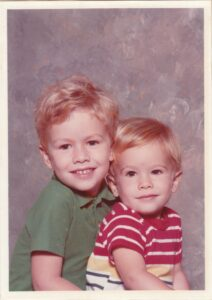
\includegraphics[width=4.53cm,height=6.392cm]{a20120403TheSonofDuty-img001.jpg} 

The delights of in the earth

The delights in the fire

The delights in the waters of living beings,

Greater than these is that of a father in a son

A son is a light in the highest heaven.

The gods said to men:

A sonless one cannot attain heaven,

All the beasts know this

This is the broad and auspicious path

Along which men with sons fare free from sorrow. 

\end{quotex}
\emph{This is how our ancient Aryan ancestors actually lived}. The \textbf{Aryan gods} advised a man to have sons; this is not just an aberration of the Catholic god as Evola insinuates. Yes, but not just the gods, even the beasts know as much. So in criticizing the family, Evola stoops lower than the animals.



Besides love and joy, there is a third factor: a sonless one cannot attain heaven. It is not just a question of continuing a biological line, but more important is the continuation of a spiritual tradition.

Now a man may sacrifice his family life to focus on a spiritual life or even, perhaps, a secular order (which Evola claimed existed) of unmarried men. Of course, once a man has fulfilled his ``duty", he may choose the celibate life of a sannyasi. But in Evola's conception, these choices hardly count as a sacrifice. Now this is counter to what he writes in \emph{The Metaphysics of Sex} about marriage. This is summarized by his quoting \textbf{Louis Claude de Saint-Martin}:

\begin{quotex}
If mankind knew what marriage is, it would have at one and the same time an extraordinary desire for it and a tremendous fear of it; for by means of it man could once again be made like God or could end in total ruin. 

\end{quotex}
Pace Evola, we believe Saint-Martin understood perfectly well what he wrote, but that is a topic for another time.



\flrightit{Posted on 2012-04-03 by Cologero }

\begin{center}* * *\end{center}

\begin{footnotesize}\begin{sffamily}



\texttt{apeiron on 2012-04-05 at 19:29 said: }

Leonidas picked the famous 300 Spartans on the predicament that they had a ``son of duty" to their name. So some of the most celebrated heroic band of solar men in Western history, procreated. Today, the act of familial procreation is seen as a bourgeois ``facist" institution by the left and as ``judaic familial values" from the ``new-right". How is this a healthy or even functional view of our ancestral destiny if this is the layman's view and not that of an exceptional and vocational spiritual type? 

I believe Evola also deliberately confuses the old testament quote of ``go forth and multiply" to the lower type of materialist man. In saying this however, we're left with the beings of sacrifice, the celibate saints, priests, holy-men and mystics who actively chose the sterile life to center their energies entirely towards god/godhood. What are we to make of that tradition (even though Evola actively chose not to be traditional as demonstrated on this site) ?


\hfill

\texttt{Angolmois on 2012-04-11 at 05:44 said: }

Marriage and children is a university / school of spirit, as the ancients knew it. For many people it would be a very good school to learn essentials of spiritual and religious life, such as (self-)sacrifice, commitment, focusing of sexual and erotic energies (for the wellbeing and integrity of one's own constitution), and so on.

There's is nothing inherently bourgeois in family life and having / raising children, but I do understand why spiritually inclined people don't marry and / or have children; especially in this age of decline and anti-tradition family – society, civilization at large – is not what it was in the past, and it can be both a spiritual and a practical, financial burden because of reasons too many to even mention in a short comment; our crumbling civilization does everything in its power to kick people with children and healthy family values to the drain. Of course there's always the possibility of keeping the flame of tradition (and bloodline) alive in one's own part, but is this the best way to do this, and not just the most wishful thinking that one can engage in?

This is why I understand Evola's views about marriage and children very well. It should also always be remembered what Evola meant by his words and writings, and to whom they were first and foremost aimed at: for men, warriors and sages of tradition.

I believe Männerbunds were not homosexual in nature – they were a-sexual – beyond sex.

If someone discards the bible as a whole on the basis of ``semitic values", they certainly have not read their New Testament through.


\hfill

\texttt{Cologero on 2012-04-11 at 07:42 said: }

I wish I could accept that, Angolmois, but this shows Evola's naïveté. First of all, he was no warrior and no sage. Granted there may be some men who choose an ascetic path early in life, but in the normal course of things, that choice is made after having fulfilled one's duties. In ancient Greece, the indomitable phalanx was manned by father and son, uncle and nephew, fighting beside each other, not by celibate warriors.

Despite all his talk about loyalty, fidelity, and authority, Evola committed himself to nothing; not to his own nation, not to his leader, not to any specific Tradition. He unfairly criticized the great philosopher Giovanni Gentile who, unlike Evola, did not philosophize in a vacuum. He raised a family, had a worldwide reputation as a philosopher, and participated in forming the Italian government, specifically in the reform of education (something Evola only talked about).

When the Nazis kidnapped Mussolini and formed the ill-fated Salo Republic, Gentile followed him, although he had nothing to gain; the Allies would have treated him gently. Against the advice of his family, he understood what loyalty meant. After the war, Gentile was gunned down in the streets of Florence by Communist partisans. Meanwhile, Evola remained behind in the safety of Rome. When the allies came looking for him, his mother helped sneak him off to Austria. Try to convince me who was the real man.

He advocated birth control for the women to be abused by the Mannerbund. Where did he expect them to come from, if a woman was under the protection of fathers, brothers, and then husbands? Apparently, from the Bohemians, or perhaps slaves from other nations and races. Apparently, he couldn't conceive that birth control used in that way led to the feminism he decried. Paradoxically, it also gave every Western man the same privileges with women that he would have reserved to the mannerbund.

The final effect of Evola's anti-family tirade is that it has brought some unsavoury figures into the sphere of Tradition, the sort of male that would never have been allowed in Traditional leadership.


\hfill

\texttt{Angolmois on 2012-04-12 at 04:08 said: }

You are right about many things, Cologero. I if anyone do not look well many Evola's views about women, which were quite harsh, dangerous and abusive. He certainly was ``too solar" in his emphasis, and this shows everywhere in his thinking and in even in his fate.


\hfill

\texttt{Sparrow on 2015-04-06 at 00:40 said: }

While your criticism of Evola is harsh, I can't help but find myself in full agreement, Cologero. A lot of these same observations came to me when reading his works, before finding Gornahoor. Despite his intelligence, or possibly because of it, Evola lacked good sense, and could be an incredibly argumentative, hypocritical, and selfish person. His sexist views on women (I don't mean ``sexist" in the liberal sense, where acknowledging difference between the sexes and supporting gender roles makes one a ``misogynist.") seemed ironic to me, considering it was certainly not to his detriment that his mother distracted Allied agents long enough for him to sneak out the door. He couldn't be pleased no matter what anyone said or did (e.g he didn't hesitate to mockingly criticize Guenon).

It is incredibly pedantic of me, but I feel the need to point out that Gentile was not killed after the war. He was killed in 1944. Ironically, he had been arguing for the release of anti-fascists (guess that's like petting a rabid dog, only for it to bite your arm off). Goes to show what happens when you attempt to show compassion to those of the Leftist persuasion.


\end{sffamily}\end{footnotesize}


\chapter{Bharat Khant. Vedic civilization}
\section{The Great Migration}

Due to the cooling of the arctic region, the Boreans were compelled to migrate southward. This probably accounts for the legends of wars against the Meridionals. \textbf{B. G. Tilak}, in his book \emph{The Arctic Home of the Vedas} estimated this to have occurred around 8000 to 5000 BC.

\paragraph{Vedas}
Tilak bases his theory on the internal evidence of the Vedas, the sacred books of Hinduism. In particular, Tilak noticed in them astronomical phenomena that are compatible with life in the Arctic. There are four Vedas written as long poems in an archaic form of Sanskrit; they are considered to be revealed scripture, and all orthodox systems of Hindu philosophy are based on them, or the Upanishads, an extension to the Vedas. Tilak considers their origin to be beyond time, hence he traces it to the Hyperboreans. Tilak writes:

\begin{quotex}
There is no reason to doubt either the competency or the trustworthiness of the Vedic bards to execute what they considered to be their scared task or duty, viz., that of preserving and transmitting, for the benefit of future generations, the religious knowledge they had inherited from their forefathers. … what is achieved in more recent times can certainly be held to have been done by the older bards in times when the traditions about the Arctic home and religion were still fresh in their mind.

\end{quotex}
\paragraph{Poetic Consciousness}
As was previously mentioned, caste structure was being established during this period. The tradition embodied in the Vedas was entrusted to the Rishis, which means ``seer". The rishis were still able to remain in direct communion with the supernature. Tilak writes:

\begin{quotex}
We may safely assert that the religion of the primeval Arctic home was correctly preserved in the form of traditions by the disciplined memory of the Rishis.

\end{quotex}
Nevertheless, the lower castes still retained features of the Primordial State. In particular, their consciousness was still motivated by poetry, rhythm, and command, rather than discursive thought. This left them with the power of concentration and great energy, since they were free of the energy-sapping phenomena of boredom, anxiety, daydreaming, and so on. Tilak explains:

\begin{quotex}
The hymns were public sung and recited and the whole community, which must be supposed to have been interested in preserving its ancient religious rites and worship, must have keenly watched the utterances of these Rishis.

\end{quotex}
Now these recitals would have gone on for hours, if not days during certain festivals. Besides the Vedas, there would have been legends and myths, some of which were probably adapted to the Mahabharata and Ramayana. Vedic Sanskrit was a syntactically complex and semantically rich language; because of its difficulty, it is accessible in the West only to a small pool of the highly intelligent and educated. Yet, during the Vedic era, the masses were in rapt attention to these recitals.

We can see the decline in later periods. The Cistercian monks chant 30 psalms per day, completing the cycle of all 150 psalms in 5 days. St Bernard said that was in concession to human weakness, since all 150 psalms should be chanted every day.

Shakespearean plays were intended for popular audiences, yet only high-brows will pay to see one today. Even as late as 19th century England, certain poets were ``rock stars"; people would wait in anticipation for a new poem from Tennyson.

In our time, the closest we have is a rock festival. Yet, sensory overload in the form of sex, drugs, loud noise and light shows are required to hold the attention of an audience. Even at that, the appeal is always to animalistic and emotional states, not to awaken higher intellectual states as in the Vedic recitals.

\paragraph{The Warrior Caste}
Nevertheless, as time goes by, the issue of castes is altering consciousness. Herman separated the venerable men and selected the warriors. For this system to persist, the question of the membership in the castes would arise again. In better times, when men were free of personal ambition and were in organic relationships, the question did not arise. Over time, the rishis were no longer seers, but became mere scribes, repeating the old hymns and texts by rote.

In the Mahabharata, the problem of membership in the warrior caste is revealed. \textbf{Ekalavya} was a man of low caste who, nevertheless, trained himself to be the best archer in the land. When he approached the martial arts teacher, Drona, about being admitted to his ashram, Drona ordered him to cut off his thumb. Of course, without his thumb, Ekalavya could no longer draw his bow. Another element is that Ekalavya was of mixed race, which was probably the reason he was excluded.

Thus we come to the end of the second age.



\flrightit{Posted on 2011-01-13 by Cologero }

\begin{center}* * *\end{center}

\begin{footnotesize}\begin{sffamily}



\texttt{kadambari on 2011-01-14 at 09:10 said: }

``Another element is that Ekalavya was of mixed race, which was probably the reason he was excluded."

Western interpretations of Ekalavya are interestesting. He was not accepted because he was not a Kshatriya. Other characters in the Maharbharata are also rejected, for example, Karna, is of divine origin in the story, but has been raised adopted by a charioteer, so he is unable to duel with Arjuna which is reserved only for Kshatriyas. No one mentions his race really, but humble background as they think he is the son of the charioteer when he is not.

Eklavya probably came from those tribes that had not been Sanskritized. It is not so much as being of ``mixed" race, but of not being of a clan which recognizes the Vedic rites and culture. The story proves that men can be human and flawed and it is Ekalavya who is the hero at the end, and Drona appears mean minded. The fact that they wrote about these things even back then shows that people were aware that caste can be problematic in some instances in excluding worthy people.

Draupadi the wife of the Pandavas is known to be extremely dark skinned so her name is Krsna which means dark, and Krishna is often represented as black. So there are exceptions. Also tribals being people who are not a part of the Vedic clan and do not follow Vedic culture, could be of all colors and variety as Hindu culture encompassed a great area back then.

For example, the royal clan of Rajputs who are known to be handsome were tribals initially and outside Vedic culture, and not original Kshatriyas. They seize power and draw up geneologies for themselves as descending from the original Kshatriyas…So these things are not as simple as people seem to think…


\hfill

\texttt{kadambari on 2011-01-14 at 09:47 said: }

Also I forgot to add that Tilak was a Hindu nationalist and not a scholar. It was not uncommon for Hindus to just accept what was fashionable amongst the indologists back then. Many more things are known today than in his time as a result of scholarship… 

One interesting thing is the people of Kailash. People think that they are the remnants of Alexander. They are not. The are remnants of the original Vedic pagans who were not Sanskritized. There were many such people in Afghanistan, tribals who were not Sanskritized, but these people were forcibly converted to Islam as recent as in the 1800's. However, in Afghanistan, the Hindu royal clans and ethnicity were completely wiped out and the people today are descended from Turko-Mongols and other people from the Middle East, and are not of the same lineage as when Afghanistan was Hindu. Draupadi the princess in the Mahabharata is known to be from Gandhahar (modern day Afghanistan). So was Panini who wrote Sanskrit Grammar. Back then, Afghanistan was a part of greater Kashmir.


\hfill

\texttt{kadambari on 2011-01-14 at 13:14 said: }

``3.Kadambari: I have understood that Krishna's name ``black" is a title which refers to the fact that he represents the unmanifested Self as Arjuna refers to the empirical ego-self. Your interpretation of them seems to be largely historical, am I right?"

I understand that. I am not saying that Draupadi was black, but simply that she is known to be very dark in the Vedas. So all these things were not as strict as one thinks, its not as if people liked only blondes and so on. Obviously in North India in those times from where our culture arises, people were generally fair and sharp featured, but color is more complex than what we understand it in modern times. For instance, it used to be common for Kashmiris to be grey eyed red haired, but no one thinks they are superior just because they are fair and so on. This is what I am saying. I think the idea was to have the Vedic clan values. Many fair peoples in those areas were also tribals and were not Sanskritized, such as the remnants of people in the Kailash who still worship Pagan gods, these people would not be accepted simply because they are fair and so on. I am sure Sanskritization of various ethnic groups took place over a large period of time.

I recently came across people from Andhra. They are black but incredibly educated and gentle people, quite unlike what one associates with blackness in the West, with stable families and values.

Also regarding those simple remnants of tribals that got converted into Islam in Afghanistan in the late 1800, I feel their fate would have been much better if they had come under the HIndu fold gradually.

As for Dalits and so on, as I said, people had come up with religions that gradually tried to absorb these people without destroying the traditional structure such as Buddhism. Unfortunately, after the Islamic invasions, Hindus do not have time to think of their fellows and become incredibly orthodox, this was a means of surviva. One has to understand that the destruction that took place is so unsettling and massive, it is hard for a culture to reassert itself in this kind of circumstance. I think classical civilization survived in the South until the sixteen century before the destruction of the Vijayanagar empire, which is why people from the South even though they are dark can be very superior as they have those values left. The north is barbaric because of Islamic influence and destruction. We say all the thug values came into India from the Middle East.


\hfill

\texttt{kadambari on 2011-01-14 at 13:44 said: }

@Ismo

Also what I mean by Sanskritization is shown by the Rajputs who were famous for their beauty and chivalry. They were tribals who became Sanskritized fairly late in Indian history, they are not the Vedic Kshatriyas, although they claim their lineage to be, they were no less brave. Kind of like what Goethe said about Shakespeare's Julius Caesar, ``They are all thoroughly Englishmen but the Roman toga suits them well…". Rajputs would fight to the last man and when they knew they would be defeated, their wives and children would commit suicide and embrace sandalwood flames they would go into battle with the ashes of their cremated family on their foreheads. Later they become corrupted and gradually give in and begin to give their daughters to Muslims rulers as they cannot expel them but not all Rajput clans do so. They were always brave, but their weakness was that they quarreled amongst themselves instead of uniting in the face of the enemy.

But then most of India's aristocratic classes were exterminated or converted during the invasions.

But still you have to understand that when Islam overran most of Asia, it was not able to convert the Hindus so easily. And today a vast Islamic population is still a hindrance to India's growth by virtue of the fact that the culture is regressive and does not assimilate to the majority like other groups.


\hfill

\texttt{kadambari on 2011-01-14 at 16:57 said: }

Ismo,

I know that this is out of context, but I could not believe it that 100,000 British have converted to Islam so far, most of them women. Recently I read an article in the Times that thousands of British girls were being sold into the sex trade by some Islamic gang. And Tony Blair's sister in law is said to have converted and wears a scarf. Seriuosly, what is wrong with these folks?

As for tribals in Afghanistan I was talking about, the place is Nuristan, formerly called Kaffiristan, land of the infidels! There were still some tall blue eyed pagan non Hindu Afghans till the late 1800's but they all got converted to Isalm. I really feel sorry for some Afghans I see on TV. Many of them just seem simple hill people who ended up brutalized by the wrong religion!


\hfill

\texttt{kadambari on 2011-01-14 at 19:52 said: }

Ismo,

Even the Dravidian Hindu city of Vijayanagar was so magnificent existing as late as the sixteenth century, it was completely destroyed by a force of Muslim rulers surrounding it, and rendered uninhabitable, today one sees only the ruins, and even those are impressive. This marked the end of classical civilization in the South. On the glory of Vijayanagar, a Portuguese traveller writes: ``The city is as large as Rome and very beautiful. It is the best provided city in the world."

When one sees the ugly cities in India today overcrowded and unplanned, it is quite hard to believe that cities like this existed not too long ago…


\hfill

\texttt{kadambari on 2011-01-15 at 11:39 said: }

Ismo,

I mentioned the Dravidian city of Vijayanagar because it was the last Hindu stronghold and a great city. Real Hindus are a tiny minority in India today, thas is, Hindus who understand their civilization. Vijayanagar was a Dravidian city, but it was based on classical Hindu ideals of heirarchy and so on, that is, the role of Kingship and priesthood is that which is defined by classical Indian civilization. This shows that the ``idea" can have different manifestations in different contexts.

Also, it is worth noting that Eklavya is a hero in the story not because he tries to destroy the Drona's order because it is unfair to him, but he shows that he is fit for it, by exemplifying its ideals to the fullest. He is said to meditate on Drona, that is, internalize the ideals which Drona represents, which is what makes him what he is.

Also of interest is the student teacher relationship that is exemplified in the story. Eklayva still considers Drona his teacher (Guru). Now the Guru in the traditional sense is held in the highest regard. He taught his students free of charge and at the end before the students would depart, they would give a gift to the teacher which is voluntary called ``Guru-dakshina". There are interesting legends about how students would value their teacher to such an extent that they would be ready to give anything to the teacher in exchange for the knowledge he imparts, and Kings lose entire kingdoms in the Mahabharata as they wish to keep the word to the Guru and give him what he demands…Now it is in this context that Eklavya gives his thumb as ``Guru-dakshina" as Drona asks for it and he has told Drona that he will give him whatever he desires. It is interesting that in these legends, importance is given to keeping one's word, no matter what difficulties it causes. Truthfulness is valued, there are tales of heros who never tell a lie and so on. The Mahabharata is full of hundreds of tales, and is to Hindus what the Iliad and Odyssey was to the Greeks.

At the end, if anything, the tale of Eklavaya shows that Drona's action was unjust, and that Eklavya is noble. Even Drona ultimately repents for his sin (asking for Eklavya's thumb).


\hfill

\texttt{Will on 2011-01-16 at 12:09 said: }

I am very unfamiliar with the Mahabarata, but I have heard this story before. It seems to me that, like myths in general, it is subject to multiple levels of interpretation, depending on who is being taught, or what is being taught, and perhaps also when someone is being taught, i.e. in what Age. 

What strikes me is that Eklavya is absolutely certain that to be an archer is his destiny and that Drona is his guru, so much so that Drona's rejection of him doesn't change this at all. So then he makes a statue of Drona and relates to that as his guru, such that when he is asked where he learned to be an archer, he does not claim to be self-taught, but rather says that Drona taught him. 

The guru is a personification of a higher power, because it's easier to relate to another human being than to the Absolute as such. But it seems that Eklavya, through exceptionally pure devotion, was able to connect with the higher aspect of his guru, even though outwardly he was rejected.

This is about the nature of devotion, sincerity, and perseverance. It's like the Buddhist story of the old woman who worships a dog's tooth, believing it to be a holy relic, and becomes enlightened. It's said that authentic devotion to a phony guru is better than half-assed devotion to a fully realized master. I don't know if Drona is supposed to be a phony guru or not, but from Eklavya's perspective, it doesn't matter, because his devotion is pure.

In the West, there is a lot of confusion and misunderstanding of the nature of the guru-disciple relationship, because we don't really have a corresponding relationship in our own sacred traditions. (Though there are traces of something similar among the ancient Greeks, such as the story of Plotinus and his master.) And the fact that more than a few Easterners have taken advantage of our naivete on this matter doesn't help.


\hfill

\texttt{kadambari on 2011-01-16 at 13:45 said: }

``I don't know if Drona is supposed to be a phony guru or not…"

The Mahabharats is amazing to read, although ten times the size of the Iliad and Odyssey. One never gets bored reading it though.

No Drona taught the princes the arts of war was was superior in his knowledge. The story just shows his human side, he also does not hesitate to favor his son, although he is not a Kshatriya, and shows other weaknesses. I suppose that these stories are interesting because they show the human character in all its forms, the strong aspects and the weak.

``It seems to me that, like myths in general, it is subject to multiple levels of interpretation, depending on who is being taught, or what is being taught, and perhaps also when someone is being taught, i.e. in what Age. "

I do not think so, people have always been clear on the meaning of these stories, the glorification of a noble character is not hard to miss. The only times they are misintrepreted is when Brahmin haters use it to show that they were cruel in a one sided way, or to justify such actions today. Again the story just shows Drona's weakness, he is a great teacher, but he also has some human failings.


\end{sffamily}\end{footnotesize}


\chapter{CJK politics}
\section{The Political Philosophy of Confucianism}

\begin{quotex}
\textbf{OKAWA Shumei} (1886-1957) was a Japanese religionist and class-A war criminal. In 1942, after the bombing of Pearl Harbor, he wrote an introduction to Islam and translated a book about the ``perennial wisdom". He was arrested by the Americans for his political leanings and faced certain execution. On the first day of the Tokyo Trials, upon entering the courtroom he yelled randomly in German and slapped Prime Minister Tojo on the head, and was shortly found to be insane. While in the mental hospital, he made the first Japanese translation of the Qu'ran.

In this essay, which first appeared in the magazine\emph{ East Asia }in October 1930, Okawa advocates for a radical break with Western political thought by reviving and revitalizing Confucian order.

\end{quotex}
To aspire to Confucianism is without a doubt to make clear the Tao. And since the Tao is nothing if not a principle for individual life, Confucianism is an attempt to expound how men might live a righteous life. Now, a righteous life is a principle that realizes the correct relation between what we call ``I" and what we call ``not I". Confucianism divides what is ``not I" into the Three Powers, Heaven, Earth, and Man. This is the Tao of Confucianism. To be precise, Confucianism is the principle that realizes the proper relations between Heaven, Earth, and Man. In China, the scholars considered least worthy were thought of as ``lacking knowledge even of the Three Powers". When the English poet Wordsworth versifies on the necessity of holding a proper idea of God, Nature, and Man, it corresponds to this precisely.

\begin{wrapfigure}{rt}{.3\textwidth}
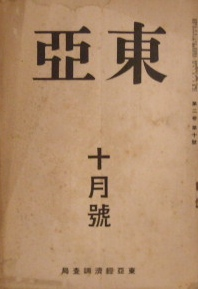
\includegraphics[scale=.5]{a20130223ThePoliticalPhilosophyofConfucianism-img001.jpg} 
\end{wrapfigure}

Now, Confucianism teaches that he who accords to Nature knoweth the Way. Mencius says that ``you must possess the five virtues yourself and extinguish your selfish nature", and this means the same thing. The autonomy of morality, which Kant outlined so carefully with his utterly precise logic, was not a unique discovery of the German philosophers. The Confucians rapidly grasped this truth based on their depth of experience. For example, Mencius' Four Sprouts are none other than a study of the foundations of human morality. What he calls a ``Sprout" is a ``natural foundation" from which morality can be grown. And so, in Confucianism, to work for ethical completeness is called development, or self-growth, or self-discipline. This capacity is inherent in oneself–he who possesses infinite possibilities for future action must start with an education in what is good. Therefore, the Tao as it pertains to Heaven, Earth, and Man first and foremost is something that should be realized through growing the natural foundations of morality in the self.

What is Heaven? Heaven is the origin of our existence. Most directly, this is our parents, and above them is our kin and ancestors. The origin of our ancestors is in the race, and the origin of that is in the universe. The correct relation to hold towards Heaven, that is to say, ``religion", is called in Confucianism Honor. This means growing and refining our essential human feelings of reverence and respect.

What is Earth? It is Nature as regarded by the mind. The most personal encounter we have with this is through our physical bodies, as well as the accompanying feelings of desire in our minds, as well as the external changes that these desires demand. The correct relation to hold towards Earth, meaning first the establishment of control over one's mind with regards to nature, and second the unification of one's attitudes, which may narrowly be called ``morality", is called in Confucianism Right. This means disciplining and training the essential human sense of shame, so that we will face towards Heaven unashamed and have good expectations for our life on Earth.

What is Man? Men are the individuals of good character whom you value equally with yourself. A well-bred man reasons with logic and acts with morality. Using logic, he understands the limitless possibilities of the complete knowledge of the universe, and thus is endowed with infinite possibility to realize in our lives, according to our intentions, the meaning of all things that it is possible to know. This personal limitlessness is called in Confucianism ``natural intellect, natural ability". Therefore, the proper relationship towards Man is to constantly develop the capacities of our natural intellect and ability, to our mutual benefit. Saying that this is realized through a purification of our natural tendency for sympathy and sentiment, Confucianism calls this Virtue. However, the collective effort to develop many intellects and abilities according to the parts of each and every life of many human beings in community is usually called politics. That is to say, the term politics is nothing other than an attempt to objectivize, or systematize Virtue.

Confucianism is therefore a Tradition that clarifies the three interests of religion, morality, and politics. Rather than breaking up these three ideas into separate fields of specialization, it understands them to interoperate as a single whole, and endeavors to eluciate the ``Tao" as a principle for all human life which contains all three. This is a point which has caused much outside confusion about the nature of Confucianism. One [Western Orientalist] will claim that Confucianism is a moral teaching, another will claim it chiefly conveys information about government, while still another lists it among the world's religions, but all their interpretation began from this source. For example, one Prof. Douglas calls Confucius' teaching nothing more than ``a plain, matter-of-fact system of morality". But Confucianism is not a religion in the Western conception of the thing, nor is it ethics or political science. Confucianism is not a single one of those, but is indeed all of them at once. Recognizing this as an internal structure, we can resolve the external confusion: this is a Tradition which we will understand nothing of from a Western perspective.\footnote{A postwar revision, and further thoughts on the concept of ``religion", can be found on my website: \url{http://avery.morrow.name/blog/2013/02/the-tao-of-the-east-and-the-last-samurais-testament/} }

\begin{quotex}
Here, \textbf{OKAWA Shumei} begins to make his departure from the basic principles of Western political thought obvious, deploying a slightly Hobbesian character from the 3rd century B.C., and demonstrating his Confucian orthodoxy. It is interesting to consider this contrast of rules vs. rulers in the modern cases of businesses, schools, etc.

\end{quotex}
The political thought of Confucianism is built on top of this fundamental spirit. Accordingly, most orthodox Confucianists could not be made to target politics as a thing standing alone and separated from religion and morality. The personal training for politicians, given names like ``study of ethical use of authority" and ``way to a virtuous nation", was never a thing separated [from the basic texts and principles]. According to Confucianism, as politics is the embodiment or systematization of Virtue, so the most essential basic requirement of the politician is to amass much virtue in their hearts. So most Confucian political works are expositions of knowledge intended for the ruler or politician. That is, to explain to the ruler the correct attitude for his heart, and how to attain virtue and compassion in his heart, is the basic method of Confucian political science.

For example, the Han \emph{Treatise on Punishment and Law} states, ``An ancient saying has it that even if the whole room has been eating and drinking, if there is one person crying to herself in the corner, no one in the room can enjoy themselves. And for a ruler, just like the case of that room, if even one person in his realm is treated unfairly, one's heart takes pity." An edict of Emperor Zhang of Han states, ``The sovereign must treat the people as if he were their father or mother, answering hardships with love, teaching loyalty and virtue, and administering appropriate punishment." Throughout the \emph{Shi Jing}, the ruler is portrayed as the mother or father of the people.

Indeed, as a consequence of understanding politics as the embodiment of Virtue in this way, the political ideal of Confucianism can be summarized in a phrase as ``domestic tranquility". Domestic tranquility means that for all of the people that exist in a nation, throughout their lives, negatively speaking they meet with no obstacle, or positively speaking, they are able to fulfill their respective functions. Nevertheless, regardless of the institution or organization, the expectation of true domestic tranquility does not mean that it is rigidly enclosed by [bureaucratic] considerations. At the top of Xunzi's thesis on sovereignty, he uses the phrase, ``\textbf{Rulers, Not Rules}``. And this phrase is the single clearest declaration of Confucian philosophy as it relates to systems and organizations, meaning that the aim of politics is not the \emph{rules}, but the \emph{character of the politicians}. Indeed, Xunzi's full statement is as follows:

\begin{quotationx}
Not a country in disorder, but a leader in disorder; not rules of order, but rulers in order. The methods of the archer Yi are not lost, yet such an archer does not appear generation after generation. The laws of King Yu of Xia still exist, yet the Xia could not continue their rule. Thus, laws cannot stand alone. Categories cannot apply themselves. If there are good men then the nation will survive. If there are no good men then it will be lost. Laws are the sprouts of order, and the man of virtue is the field in which that order grows. If men were virtuous enough we could even do without laws, but if no man is virtuous, no laws will suffice to save us, and we will fall into disorder. One who can simply count off the laws without knowing the Right behind them, no matter how learned you might call him, if he is given authority disorder will result. Therefore, a good king goes swiftly in search of good men, while a bad king seeks out power.

You ask how to rule a nation. You should first ask how to discipline yourself, before you can run a nation. The sovereign rules, and with his right rule comes right views. The sovereign is a bathtub, and his people are like the water. Water follows the shape of the tub. If he is a round tub, they will be round, and if he is a square tub, they will be square. It does not matter if it is the sovereign's edicts or his mere whims. King Zhuang of Chu preferred slender bodies, so there was starvation at court. If you must ask how to discipline yourself, you do not yet know how to rule your nation.
\end{quotationx}

Mencius means the same thing when he says frankly that ``without men of virtue, there can be no rule", and a famous chapter from Confucius' \emph{Doctrine of the Mean} goes, ``The government of Wen and Wu is recorded on tablets. Let there be such men and the government will thrive; but without such men, the government decays. With men who heed the Tao, government flourishes, just as agriculture flourishes when the Tao of the Earth is heeded; indeed, government matures just as reeds shoot forth from the soil," expressing the same idea.

The theory being expounded in \emph{Doctrine of the Mean} is as follows. An ideal government existed in the time of Kings Wen and Wu, which can be verified through various documents. People like them can govern splendidly, but without people like them, good governments can crumble. If good people are promoted to government, it is like plants growing from rich soil, and the results will come quickly. The rise and fall of individual politicians has immediate consequences in politics, just as a sudden change in soil quality has an immediate influence on the plant. Regardless of political system, our politics depends on the character of the people in it. And the type of people who will be appointed depends solely on the character of the ruler. Moral principles must be protected to establish good character. And virtuous love must be cultivated to possess those moral principles.

\begin{quotex}
Translation notes: The term ``man of virtue" means an educated elite, and is similar to how Julius Evola employs the term ``Aryan".

The Confucius translation is adopted from several English sources, rather than Okawa's incomprehensible late medieval transliteration (which he re-translates in the next paragraph). The first fourth of the Xunzi translation, about the archers and the Xia, is derived from Kurtis Hagen, \emph{The Philosophy of Xunzi}, Open Court Press, 2007. The rest is original and somewhat loose, but I swear to God he really does say the sovereign is like a bathtub.

\end{quotex}

\hfill

\begin{quotex}
Now, \textbf{OKAWA Shumei} takes out the big guns, attacking the founder of Legalism as impeding the cultivation of virtue, and by implication Western political theories which aim for the same legalistic goal. What the reader might not realize is that in denouncing Han Fei, who lived in the 3rd century B.C. and had an influence on all Far Eastern political thought thereafter, Okawa is arguing for a return to a very ancient ideal indeed. When a group of ultra-nationalists tried to overthrow the constitutional monarchy of Japan in the name of direct Imperial rule, Okawa was sent to prison for five years for providing the theoretical principles for such a political concept.

\end{quotex}

This concept, the greatest conceivable system to realize human ideals in an actual nation, comes into obvious opposition with the political philosophy of the West, which attempts to induce people to march automatically, so to speak, towards progress and perfection. Western political thought, in the words of Xunzi, has ``rules, but no rulers"; that is to say, it values creating good ``laws" over creating good ``men". Even in China, some sages like Shen Dao, Yin Wen, and Han Fei value law over men in their writings. Han Fei, especially, fiercely attacks the idea of ``rulers without rules" in one of the chapters of his book, and devotes himself to organizational structure. What he claims is that waiting for a man of virtue to appear is like a hungry man refusing to eat for a fortnight while he waits for a prime rib to arrive; the poor soul will simply starve to death.

His argument goes like this: Even with a total disinterest in organizational structure, a nation can be ruled by the likes of an Emperor Yao. And even with the finest organizational structure, a nation ruled by a tyrant would quickly dissolve into chaos. But a great Emperor Yao or a tyrannical King Jie will appear only once in a thousand years. Most rulers are neither Yao nor Jie. To create a nation that can be ruled by ordinary rulers, we must create the appropriate institutions. Creating people rather than rules creates a nation that can only be ruled once in a millennia, while creating rules for people will make a nation that is only disrupted once in a millennia.

Han Fei declares this to be a truth that is difficult to deny, and indeed, if we place our faith completely in the personality of a ruler, the result will be as Han Fei describes. But in Confucianism, even if there have been some who put an undue emphasis on it, there has been no one who disputes the meaning and value of ``laws". Actually, in the \emph{Doctrine of the Mean}, the three major functions of the ruler are piety, governance, and intellect. Piety implies both religious courtesies and moral customs, while governance means legal and political systems, and intellect refers to literacy. Without grasping the aforementioned three things, one cannot be a ruler in either name or reality. Even the most earnest abstract desire for a ``domestic tranquility", without institutions in place to ensure true domestic tranquility, we would not expect anyone to call someone a real politician. Mencius says, ``Mere good intentions do not build a government, nor do mere laws." The ``mere" here means subjective, or abstract. Confucianism, therefore, does not at all ignore structure, but recognizes that spiritual development must be esteemed over mere structure.

The success of all systems is, without a doubt, the result of a success of the human spirit. Therefore the true meaning of a structure cannot be grasped by the people who join into that structure if they lack a spiritual foundation. It becomes accordingly difficult to maintain it effectively. A genius who knows all 3,000 rules of etiquette and 300 marks of majesty, if he fails to grasp the true meaning of piety, will simply fall into useless, machine-like imitations. And in order to grasp the true meaning of piety, we need true hearts and good faith. This is why Lu Jiuyuan said, ``If we fail to overcome our own selfishness, it will be difficult for us to know virtue. And without a full knowledge of virtue, we will know not what rules and regulations are for."

\begin{quotex}
I continue directly into the conclusion. Hopefully all the readers of this blog will be quite gratified to see this independent manifestation of the Traditional principles.

\end{quotex}


Now, in Confucianism, there is a strong emphasis on ``love for relatives", or ``veneration for noble deeds" as a principle for social life. In the \emph{Doctrine of the Mean}, Confucius teaches: ``The humanity of virtuous behavior is made evident in the case of love for relatives. The ability of righteousness to set things straight is made evident when we honor noble men. The decreasing measures of the love due to relatives, and the steps in the honor due to the worthy, are produced by the principle of propriety." The implication of this passage is, approximately, as follows. Virtuous love binds people together, and its most striking manifestation is in our natural affection for our parents and kin. In contrast, justice is a type of discrimination. Its most striking manifestation is when we naturally hold some sense of respect towards noble men, that is to say, those whose moral values tower above all of us.

Nevertheless, we do not love all of our relatives equally. Even if the original source of virtuous love is an indiscriminate, equal substance, it is utterly unforgivable for its manifestation to be uniform in nature. Our reverence towards ethical exemplars, too, is of the same nature. In the manifestation of virtuous love and reverence, the attempts to confer a correct order are the grounds that generate the various forms and systems of social life. It is an indispensable condition for a Confucian social order that social inequalities are generated from a correct moral foundation.

Both love for relatives and veneration for noble deeds are called much more simply ``filial piety" or ``respect for the elders". One of the first statements in the \emph{Analects} reads, ``A youth should be filial at home, and, when abroad, respectful to his elders." The model for household life necessitates recognizing the position of parents, and each sibling among the children disposes of his ``self" and faithfully works for the sake of his family and clan, continuously realizing an order of being. Honoring virtue, similarly, underlies the model for national life, and Confucius teaches that the exercise of authority both large and small necessitates a shared concept of virtue, which people must entrust to the statesmen, abandoning their ``self" interests and faithfully obeying the authority of the state.

Therefore, the duties of the men of noble birth in China were not rule of the country–personal oversight as administrators–in the usual sense, but were actually the promotion of able men to wield authority in roles both great and small. Therefore, it is said that ``if we hasten to get the right men, the self is checked and the nation is put in order, the merits are great and one's name is celebrated, and one is worthy of being called a sovereign. If we do not hasten to get the right men, but instead focus on getting the labor first, then people will work for their own purposes and divide the nation, merit is abandoned and one's name is besmirched, and the very soil and grain of the nation will certainly be endangered. The worthy sovereign seeks out the men and, having found them, may rest."

``If the people be led by laws, and uniformity sought to be given them by punishments, they will try to avoid the punishment, but have no sense of shame. If they be led by virtue, and uniformity sought to be given them by the rules of propriety, they will have the sense of shame, and moreover will become good." This is a famous saying of the \emph{Analects}, and a summary of the essential spirit of Confucian political philosophy. […] And there is one point on which Confucianists and Legalists agree. Namely: what constitutes an upright citizen, in other words the attempt to forge a tempered and cultivated political individual, is a separate matter from the legal system, in other words the attempt to establish a systematized nation-state. Again, in other words, while Legalism insists on the strictly impartial nature of legislation, Confucianism remains the first principle at the root of litigation [because the goodness of a person is based in Confucian values].

In this way the political doctrine of Confucianism is generally not called one of constitutionalism, but is rather rite-ism, and the relation between laws and rites is perfectly encapsulated by Liang Qichao, who said that ``laws treat the symptoms, but rites are preventative health." According to Confucian political science, the sole foundation of good government is indeed cultivation of culture and learning: ``right learning brings good customs, and good customs bring good government."

The political thought of Confucianism, as clearly indicated by all the histories, was never implemented closely in China. The finest implementation of it up until now was in our own nation's Tokugawa period. The shape of our nation in that era rivals and even exceeds that of China's Spring and Autumn period, showing that the political ability of the Japanese far outstrips that of Han Chinese. The China of the Spring and Autumn Period was not much different from the old shogunate in population, area, or feudal development. Accordingly, the political ideals of Confucius and Mencius, although meant for a united China, became much more relevant in our own country, and our political ability was not just a realization of those ideals but a superior realization to that of China.

Thus in the Tokugawa period, the ideal that made the sovereign parent to the nation became ingrained in the hearts of the provincial lords, and when one province achieved a temporary state of good leadership, other provinces felt a need to compete [as in sibling rivalry] and strained to achieve the same standard, creating a splendid government. That China later descended into pandemonium and confusion despite its cultivation of Confucianism is not due to any insufficiency in Confucianism itself, but the fault lies in the political incompetence of the Han.

\begin{quotex}
The pointedness of this last paragraph lies in the fact that Okawa has just made use of brilliant reformists like Liang Qichao (1873-1929), but unlike their Japanese counterparts, the Chinese reformists failed to rebuild and modernize China.

All credit for the production of this translation lies with the Okawa Shumei Study Group which made these materials available. All fault for the numerous translation errors and misrepresentations lies with me.

\end{quotex}


\flrightit{Posted on 2013-02-21 by Avery Morrow }

\begin{center}* * *\end{center}

\begin{footnotesize}\begin{sffamily}



\texttt{Lemonheadz on 2013-02-22 at 00:28 said: }

Did Okawa have any contact with Guénon or his school of thought?


\hfill

\texttt{Avery Morrow on 2013-02-22 at 00:35 said: }

Okawa unfortunately seems to have missed out on Guénon and his school. His leanings in that direction, though, are demonstrated by a book he translated for a man named Paul Antoine Richard, the husband of Sri Aurobindo's spiritual successor ``The Mother". Richard's book is indistinguishable from Aldous Huxley's The Perennial Philosophy which was written 2 or 3 years later. After long conversations with Richard, Okawa became a big fan of Sri Aurobindo despite a lack of thorough reading into his philosophy.


\hfill

\texttt{Jason-Adam on 2013-02-22 at 17:58 said: }

Honour also consists in admitting your sources. You don't learn from China and Korea and then take their women as your sex slaves and their men as forced labour. Japan behaved with great dishonour during WW2 and was punished by Heaven for it.

I strongly advise that in studying the Far Eastern form of the tradition, we should avoid the Japanese derivative forms and look to the roots in China and Korea…..

For the record let me also say that the Koreans are a much stronger martial people than the Japs, they beat the French and Americans in the XIXth century and the Japs many times over the centuries, last time being WW2.

I am presently preparing to be initiated into a Korean order…..


\hfill

\texttt{Avery Morrow on 2013-02-22 at 21:24 said: }

I can't really comment on your principle that the truthfulness of a text can be judged by the circumstances its author lived in, nor that military defeat is a sign of martial strength, but I feel obliged to at least correct your inaccurate claim of ``sex slavery"; not only was no slavery involved in Japan's military brothel system, but it was taken over by the Americans and used in the Korean War, and a similar system was set up by the Americans in Vietnam, purchasing women from impoverished Vietnamese families. Please see this academic summary of research into the subject.


\hfill

\texttt{Janus on 2013-02-23 at 17:37 said: }

I must disagree here…the extent to which a woman in poverty can really be said to be ``willing" in her prostitution is highly debatable. The amount of freedom she really had once in the hands of soldiers, Japanese or American, even more so.


\hfill

\texttt{Janus on 2013-02-23 at 17:42 said: }

The tripartite division of Confucianism presented here is interesting, but does it not focus more on the cult of the ancestors than the cult to Divinity? Or is this Divinity contained in the ``universe" which births the race, ancestors and parents?

The acknowledgement of Confucianism as an organic ``living" practice, rather than just a philosophy is essential and something I am glad to see here. The western insistence on dividing learning, work, life, religion, and so on is a major sign of its degeneration. His comment on the western perspective is spot on, although I must agree with doubts expressed about using the Japanese rather than original Chinese perspective, particularly one coming from the Imperial era of the 20th century rather than pre-Meiji Ishin.


\hfill

\texttt{Jason-Adam on 2013-02-23 at 17:57 said: }

It's a tricky matter. My grandfather was a rikuguntaisa in the Japanese army during the Greater East Asia War but after visiting Korea I feel as if I need to make penance for his misdeeds.


\hfill

\texttt{Avery Morrow on 2013-02-24 at 06:43 said: }

This is too late at this point, but I'm sorry for my rather accusatory and grumpy comment. I thought about it a lot today, and I am certain my attitude stems directly from reading too many high-tempered Internet arguments.


\hfill

\texttt{Jason-Adam on 2013-02-28 at 21:53 said: }

The author shows his racism by blaming the problems of China on racial defects and not on failures of character, failures that afflict men in all nation, and have made Japan a cultural and political colony of America since 1945.

In fact, China under the Qing dynasty was a quite stable and functional regime until the British imposed opium addiction on the Chinese people.

I see a contradiction in that the author praises Edo period Japan, which was a peaceful, feudal, and autarchical era yet he supported ultra-nationalism which was more like Fascism in supporting an expansionist centralised state under the dictatorial rule of the Mikado who was no longer the spiritual figurehead he was under the shogunate but an actual Bonaparte-type sovereign under this sytem (I'm thinking also of Ikkai Kitta)


\hfill

\texttt{Avery Morrow on 2013-02-28 at 22:01 said: }

You forget that China was not the only East Asian nation struggling with Western interference; Japan was also thrown into crisis by Western temporal power, and its response was quite different from China, while its blazing fast modernization and militarization was due in large part to the efforts of Emperor Meiji himself.

Okawa witnessed the failure of both China and Korea to adapt in his own lifetime, and the near subjugation of both nations by the West; he has ample reason for his patriotic attitude. I would wager that he is actually a more appealing figure than Evola, who discarded sentimental ties to family and nation.


\hfill

\texttt{Jason-Adam on 2013-03-01 at 18:01 said: }

Modernisation……that's the problem…….in order to fight the West, Japan became a western power. 

China and Korea failed, yes, though in the Korean case the failure is arguable as I can attest to the survival of Korean tradition through my own studies in that nation. But the failure is simply that of traditional falling to modern which is not a good thing in my book, as I'm a supporter of the old ways.

Asian patriotism like any patriotism is a good thing but not when it becomes a tool for colonialism – if Japan had led Asia against the West he'd have been heroic but instead the Japs decided to just enslave fellow Asians in Manchuria, Korea, and China.

PS – the US tried to open up Korea in 1866 the same way they did with Japan in 1853 but that time the Koreans won and the big noses came home dead…….

I prefer Evola's attitude of placing principles above false realities……he saw the true state of his Italy and did not fail to expose it…..


\hfill

\texttt{Avery Morrow on 2013-03-01 at 18:44 said: }

To try to drag the discussion back to the actual nature of this essay, I don't think Evola's political vision is that far from Okawa's, except that the situation in Italy ensured that Evola could never dream of implementing a Traditional government, whereas Okawa had many adepts hoping to do just that.


\hfill

\texttt{Jason-Adam on 2013-03-01 at 23:13 said: }

I hope I am discussing Okawa's essay here when I raise issue with the fact that he claims China never properly implemented Confucianism, I would like to know that if he is correct, then how would he describe the ruling ideology of the Chinese empire from the Han dynasty (200 BC) to the end of the Qing (1912 not counting its revival in Manchukuo, 1930s)?

The difference I am seeing between Okawa and Evola, correct me if I am in error, is that whereas Evola wanted the unification of Europe under a supranational Emperor that transcended nationalisms, Okawa believes Japanese nationalism can unify Asia under Japanese domination ?


\hfill

\texttt{Janus on 2013-03-02 at 00:31 said: }

Fascinating piece, though I must too express my disappointment at his ease in asserting that there was some racial flaw in the Han which caused the decline in China, especially when he mentions periods in Chinese history when righteous rulers came to power. 

I'm also glad to see that he discussed Legalism, the philosophy predominant in influence in China today, especially on the political stage, and that he can do so without quickly dismissing it. Political ideas and movements are revealed for what they are without men and women of quality making up the numbers: utopian ideals at most, and farces leading to tyranny at worst (see the Conservative revolutionaries, who allowed their ideas to be hijacked by those for whom Aryans were a mere biological race). It is essential to make good laws in the State, but even more to realize that they are there to craft good human beings. This is the most radical assertion one can make in the political and social realm, and a dangerous one which can lead to tyranny if there is no direct and positive correlation between position in the hierarchy and standard of character and accountability. 

I heard two quotes in a performance of the Trial of Socrates which I think beautifully encapsulates the Confucian view in a democratic context: ``In a democracy, you're only asked to do two things: obey the law, and try to change it if you think it's wrong." and ``You accepted the constraints of the law every time you accepted our protection and did not speak in the Assembly in order to craft the best laws possible." Without good and just men, there is no good and just order.


\hfill

\texttt{Avery Morrow on 2013-03-02 at 05:09 said: }

What was actually implemented from 200 BC to the 1930s was Legalism, which was argued in this essay to be a distortion of the original tradition. (In the same way that the Christian medieval world was a distortion of the Roman imperium? Maybe? Hmm.)

That's a great question. I honestly don't think Okawa had such a naively imperialist view, but his geopolitical analyses are yet on my to-read list, and if I translate anything else by him on Gornahoor I will mention what I learn.


\hfill

\texttt{Jason-Adam on 2013-03-02 at 17:32 said: }

@ Avery

It would be good to read more of Okawa's ideas, as the close relationship between geopolitics and tradition is something I feel Guenon and Evola did not see…………

It's very interesting, the subject of Legalism, I remember reading once someone tried to argue that Maoism is actually derivative of Han Fei Zi, it is true that to some degree Mao admired Qin Shi Huang, the persecutor of the Confucians…… 

In a western context, do you think Plato is closer to Confucius or Han Fei ? The fact that he wrote a book of Laws seems to indicate P. thought he could legislate for a state beyond the capabilities of individual men ?


\hfill

\texttt{Avery Morrow on 2013-03-02 at 18:35 said: }

Just as a particular example, I think Plato's belief in the communal upbringing of children puts him squarely on the side of a Legalist legislating morality. That's not to say this idea is horribly dangerous, since Israel's kibbutzim implemented something like it and did not end in disaster. Nor is Legalism anti-Traditional; the early modern period was full of such attempts to preserve exoteric manifestations by putting them into law.

But the Roman imperium was not characterized by a huge list of laws and a great bureaucracy maintaining them. People's instincts for things like raising their own families were considered to be basically good, and only needed cultivation through education. I think Okawa and Evola are both right to claim that in the ``world of Tradition", Law is only expressed through obedience to the Principles, which are self-explanatory and within every human heart.


\hfill

\texttt{Avery Morrow on 2013-03-02 at 23:28 said: }

One last note: if anyone would like to flesh out their knowledge of Xunzi I found a Ph.D. thesis which supports Okawa's thesis that Xunzi defended real Confucianism from Legalism, actually closely imitating the conclusion that Confucianism supports the concept of laws but Legalism turns this into an obsession.

http://scholarspace.manoa.hawaii.edu/handle/10125/3023

Excerpt: ``While Confucian constructivism can support a theory of universal human rights, if it is to remain Confucian, it would not emphasize this because Confucianism perceives reasons not to foster a strong rights culture. Rights are viewed as legalistic mechanisms which, if over-emphasized, can erode informal mechanisms such as Ii (ritual propriety), the maintenance of which is considered critical to maintaining a healthy society. Citing several passages from the Xunzi, along with other Confucian texts, Ch'ii T'ung-Tsu concludes: `Confucians firmly believed that … The order or disorder of a state … depends completely upon the maintenance or the decay of li' (Ch'u, p. 241). To the degree rights seem to undermine rites, they will likely continue to be resisted."


\hfill

\texttt{Jason-Adam on 2013-03-02 at 23:57 said: }

Avery, so in your view one can be a Confucian or a Legalist and still be Traditional ?

Would you define the Torah or the Shariah as versions of Legalist thought ?

I wonder if the purpose of Confucianism and Legalism are for different ages, the age of Yao and Shun compared to our time from a Hindu perspective is different points and the cycle and different styles of governance perhaps may be required ?


\hfill

\texttt{Avery Morrow on 2013-03-03 at 00:24 said: }

I would agree that Confucianism and Legalism are both Traditional and suited different ages, since this is grounded in historical fact as well. It's also obvious that rabbinic halakah did not exist when Israel was a kingdom (the Torah and Talmud are not solely legal texts). But shariah just as clearly comes from the ``seal of the Prophets" himself, befitting the 8th century AD.

This exchange has made me wonder much more seriously whether a ``return to Confucianism" would approximate a Protestant desire for the simplicity of the earliest sources without the awareness that we are living in a degenerate age. Evola, of course, would disagree, and there are plenty of medieval texts that assert that Confucius takes primacy over his commentators, but I would like to see what Schuon says on the matter.


\end{sffamily}\end{footnotesize}


\chapter{The Ancient City. Greek and Roman civilizations}
\section{Race and the Myth of the Origins of Rome I}

\begin{quotationx}
This essay by \textbf{Julius Evola} was originally published in the journal \emph{La Difesa della Razza}.

In the context of the recent series of posts, this can be understood as the ``Noble Lie" about the birth of Rome. From the point of view of profane history, these myths are simply superstitions. Evola, on the other hand, drawing on Vico, Bachofen, Guenon, \emph{inter alios}, views such symbols, myths, and legends as witnesses to the inner spirit of a people, which cannot be grasped simply in the accumulation of historical facts. Logically, this technique leads him to move beyond the merely physical and zoological understanding of race to the notion of the races of the soul and of the spirit. (This is a reformulation of the Rosicrucian notions of the folk soul and folk spirit.)

In this first part, Evola brings to light two aspects of the myth. First is the idea that the founder was born from the union of a god with a mortal woman. The god confers spiritual qualities on the founder. In this case, Mars, as the god-father of Romulus and Remus, is the spirit of warrior virility, not just on the twins, but on the entire city.

The second aspect is being saved from the Tiber as infants. For Evola, this represents the hero, the seer, etc., men above the flow of time.

The defect in Evola's methodology is that he is left in the same position as the profane historian: the third person perspective. Although he sees more deeply, he is still an outsider and does not participate in the myth. So, yes, for him, too, it is a Noble Lie. For the Romans, Mars was a living being, not some abstract force, and the story of their miraculous rescue from the Tiber was considered history, not legend.

Although we can get some idea of the spirituality and mentality of the Romans from Evola's analysis, a scholarly discussion cannot lead us to that same state. For that, the method of Hermetic meditation described by \textbf{Valentin Tomberg} is much more helpful\footnote{\url{https://www.gornahoor.net/?p=898}}. This is a lesson for those hoping to establish a new regime somewhere, sometime: they must create a noble lie that is also a spiritual truth. 

\end{quotationx}
In his \emph{Life of Romulus} (I,8), \textbf{Plutarch} writes:

\begin{quotex}
Rome would not have risen to such power had it not had, in any way, a divine origin, such as to offer to the eyes of men something great and inexplicable. 

\end{quotex}
\textbf{Cicero} repeats the same thing (Nat. Deor. II,3,8) and considered (Har. Resp., IX, 19) the Roman civilization as that which through sacred knowledge ``surpassed every other people and nation": \emph{omnes gentes nationesque superavivums}. Sallust called the ancient Romans \emph{religiosissimi mortales} [the most religious mortals].

On the other hand, in our day all of that is fantasy or superstition for many ``serious" persons and many ``critical" minds. The ``facts" are the only things that count for them. The mythical traditions of the ancients have no value, or they have it only insofar as it is supposed that, here and there, they are confused reflections of real events, that is to say, tangibly historical. There is, in that, a fundamental misunderstanding that was already denounced, to a certain degree by our \textbf{Giambattista Vico}, then by Schelling, still more recently by Bachofen and, finally, by the most recent school of the metaphysical interpretation of myth, and by those little known today (Guenon, W. R. Otto, Altheim, Kerenyi, etc.). According to all these writers, the mystical traditions are neither arbitrary creations more or less on the poetic and fantastic plane, nor deformations and transpositions of historical elements. Especially in regard to origins, it was correctly pointed out that symbols and legends,

\begin{quotex}
if only in a dramatized form, represent actually and truly the history of the beginnings of a nation, but not the history of events occurring materially on earth, but rather of spiritual processes that have given birth to a new people alongside other people although different in culture and civilization: history, so to say, of its prenatal period.

Legend and history are tightly connected; the former proceeds through interiorization and is dispersed through images, while the latter proceeds through exteriorization as facts and events. These images are the result of formative living forces, facts are organized by the human thought. In legends one is transported by formative forces; in the other, there is premeditated organization of facts. But the legend is the invisible part and root of history; it is not poetry, rather it is a reality much vaster than history itself. The threads of the destiny of a people that unravel visibly in the most various ways in their historical development, go back to the impulses, to the creative spheres, to which the heroes of its legends are connected. 

\end{quotex}
In a particular way, \textbf{Bachofen} revealed that even at the point in which evidence, by being recognized as a myth, came to be rejected by profane history, even when it is a positive witness to the spirit of a people.

In that way, a study of mythical traditions, using new criteria, can lead us to interesting conclusions from the point of view of a theory of race that is not defined by the material aspects of the issues, but also addresses the inner reality of race.

On the occasion of the current anniversary of the Birth of Rome, we want to illustrate this interpretative method, applying it precisely to the exegesis of the myth of our origins. The legends related to the birth of Rome concentrate such a quantity of sensitive elements based on general meanings of civilizations and mythologies of Aryan peoples, that a special work would be necessary to analyze them and clarify them adequately. Therefore, we will point out here only the most notable themes, among which are: the miraculous birth, the theme of being ``saved by the waters", the ``wolf", the ``tree", the rival pair of twins.

The myth of the union of a god with a mortal woman, in the present case, of Mars with Rhea Silvia, from which union Romulus and Remus were born, recurs in almost all traditions in regard to the birth of ``divine heroes". Zeus and Leto gave birth to Apollo, Zeus and Alcmene to Hercules, Heracles being the symbolic hero of the Doric-Achaean Aryan peoples, and Apollo having a connection with the land of the Hyperboreans and with the primordial Nordic-Aryan races. An analogous origin, in properly Germanic traditions, is attributed to the heroic peoples of the Volsungs, to which Siegfried belongs.

In the ancient royal Egyptian tradition — whose remote origin can with good reason also be considered to be Aryan, Atlantic-Occidental — every sovereign is thought to have been begotten by a god uniting with the queen: this tradition in which the hidden meaning of the myth comes to the fore, inasmuch as a miraculous birth without the help of a man, of a human father, was imagined. Since the queen had her consort, the idea that her son was conceived by a god, being awakened to life by her husband, could only indicate that he, not in his moral part, but so to say, in that eternal and ``divinatory" part, had to be thought of as a type of incarnation of a decisive supernatural element that came to confer a royal dignity on him.

In the case of Rome, therefore, Mars is such an element from above, that is, the divine representation of the principle of warrior virility. Such a force stands therefore at the origins of the Eternal City and at the basis of its secret origin, veiled by the legend: so that in some traditions from the era of the Roman Republic itself, it will be directly conceived as the ``son" of Mars. And this ``Mars" force is associated with those who may be the guardians of the sacred flame of life; symbolically: with a vestal (Rhea Silvia).

\begin{wrapfigure}{rt}{.4\textwidth}
 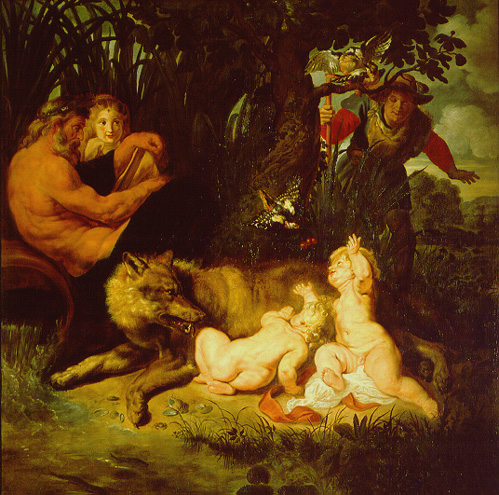
\includegraphics[scale=.3]{a20141211RaceandtheMythoftheOriginsofRome-img001.jpg} 
\end{wrapfigure}

The twins Romulus and Remus are abandoned to the waters and are saved from the waters. Here again is a symbolic theme recurring in many traditions: Moses is saved from the waters, the Indo-Aryan hero Karna is left in a basket in the river and is saved from the waters, and so on. But the symbol contained in the most ancient Aryan tradition is especially important, i.e., the Vedic tradition, in which ascetics are depicted as ``supreme natures who stand on the waters". Analogous explanations and, therefore, the hidden meaning of such a symbol, can be clarified as follows: the waters have traditionally always depicted the current of time, i.e., the basic element of mortal, unstable, contingent, passionate, fleeting life. The weak man is taken from the waters and carried from the waters. The seer or hero, the ascetic or the prophet is saved from the waters, or is capable of standing on the waters, or of not sinking in the waters. Hence, in the myth of the origins of Rome this symbol must again characterize the ``divine" element of the founders of Rome, their, so to speak, supernatural dignity.



\begin{quotex}
This is the second and concluding part of the essay by Julius Evola on the race and origins of Rome.

He points out the symbolism of fig tree, which was also the tree associated with the Buddha's awakening. The next symbol is the She-Wolf who suckles the twin babies. The wolf curiously has a dual symbolism: it can represent both the forces of light and the forces of darkness. This is often depicted as the battle between order, or Logos, with Chaos.

It is interesting to point out that the primal symbol of the wolf has been replaced in our time with the lap dog.

The spirit of Rome is exemplified by the manifestation ``of a principle of light and of order, of an ethic and a vision of life that is witness to the Aryan spirit". Here it is made clear that the Roman race is known through its spirit, not its genetics. So before constructing our Republic, it is necessary to describe that principle, ethic, and vision.

\end{quotex}
The twins find refuge near the fig tree [\emph{Ficus Ruminalis}] and are suckled by a She-wolf. The word Ruminal contains the idea of feeding: the quality of Ruminus, related to Jupiter, alluded to the quality of ``nourisher", of the ``god who gives nourishment" in the ancient Latin language. But this is the most elementary aspect of the symbol. In general, in the most ancient traditions of the Aryan races, the tree is the symbol of universal life, it is the tree of the world or the cosmic tree. If it is in form of a fig tree as it appears in the legend of Roman origins, precisely as a ``\emph{fico indico}" [Banyan tree] — the ashwattha tree — it is depicted as upside-down in the Indo-Aryan tradition to express that its roots are from above, in the ``heavens". The idea of a mystical food from the tree is a often recurring theme: the myth of Jason, Hercules, Odin, Gilgamesh, etc. Naturally, according to the races and their spirit, this then presents diverse variations. We know from the Hebraic myth that to pick and eat from the tree in order to make oneself like god is considered as the principle of guilt, abuse of power, and a curse. Things are conceived in a very different way in the myths of the Aryan races and even in the paleo-Chaldean myth of Gilgamesh. Also, in the legends of the Ghibelline Middle Ages, the heroic theme prevails and the tree often appears as that of the universal empire, reaching it in the symbolic lands of the mysterious Prester John means insuring the same dignity that the ancient Ario-Iranian rulers associated with the title of ``king of kings".

Returning to our main subject, in the myth of the twins at the origins of Rome, we therefore have the allusion to a supernatural food from the Tree — but also from the She-wolf. The symbol of the She-wolf, considered in its entirety and in all the stories that refer to it, has an ambiguous character. Lucian and Emperor Julian recall that, in the ancient world, on the basis of the phonetic resemblance between the two words, the idea of the wolf [\emph{lupo}] and of light [\emph{luce}] are often associated: \emph{lykos}, which in Greek means world, sound like \emph{lyke}, light. But there are also figurations of the wolf as a hellish animal, as a dark force. The Wolf thus appears to us in the double aspect, symbol of a ferocious and savage nature and also as the symbol of a luminous nature. This duality is verifiable, not only in Hellenic-Mediterranean prehistory, but also in the Celtic and Nordic. In fact, on the one hand in the Nordic-Celtic and Delphic cults the ``wolf" is connected to Apollo, i.e., to the Hyperborean, Nordic-Aryan god, simultaneously conceived as the solar god of the golden age and significantly associated by Virgil with Roman greatness. ``Sons of the wolf", on this basis, was a designation for warrior and heroic peoples of Nordic-Germanic origins, designations that persisted even to the epoch of the Goths and Nibelungs. Yet, on the other hand, in the Edda, the ``age of the Wolf" signifies a dark age, marking the epoch of the outbreak of savage and elementary forces, almost of the power of chaos, against the forces of the ``divine heroes", or Æsir.

Now we can certainly also relate this duality to the principle that, according to the legend of origins, ``fed" the two twins insofar as we see it reflected in their very nature, that is, in the antagonistic duality of Romulus and Remus, as related to us in the myth. As others already noticed, so also the theme of a single principle from which an antithesis is differentiated, whether depicted by the antagonism of two brothers of twins or, in general, of a couple, is found again in many traditions, and not rarely in respect to particularly significant moments for the origins of a given civilization, race, or religion. For example, we only recall that in the ancient Egyptian tradition Osiris and Set are two brothers of discord — sometimes conceived as twins—and one incarnates the luminous power of the sun, the other, a dark, ``infernal", principle, whose generation is called the ``sons of the impotent revolt". Does not something similar also show through perhaps in the Roman legend? Romulus is the one who marks the contour of the city as the meaning of a sacred rite and a principle of \emph{limit}—of order, of law—having received the right of putting his name to the city from the apparition of the solar number, of the \emph{twelve} vultures. Remus is instead the one who violates such a limit and is killed for this reason. One could say that the primordial force of Roman origins thus are differentiated and destroys the ``dark" powers that contained in themselves, affirms in its luminous aspect of order, Olympian domination, purified warrior force.

There have been attempts to see in the contrast between Romulus and Remus the reflection of the contrast between opposed Aryan racial forces, or of the Aryan type, and non-Aryan or pre-Aryan types. Research of this kind is without doubt interesting: problematic in its conclusions, if it intends to remain exclusively on the plane of material facts, or archeological and anthropological evidence. It has greater possibilities if it also penetrates the myth and legend in order to extract elements that integrate research in other domains. Naturally, in order to accomplish that, it also needs to resolve to outline general frameworks of various aspects of ancient Roman society, considering, for example, with various writers, somewhat probable that the social system of castes of ancient Rome had a racial substrate.

In this totality, it is interesting to examine the link between the two principles, whose symbolic figurations could well be Romulus and Remus, with the two hills Palatine and Aventine. The Palatine is, as we know, Romulus' hill and the Aventine is Remus'. Now, according to the ancient Italic tradition, on the Palatine, Hercules met the good king Evander (who significantly founded a temple of the goddess Victoria on the same Palatine hill) after having killed Cacus, son of the Pelasgian (pre-Aryan) god of the subterranean fire: and Hercules conquered and killed in Cacus' cave, \emph{located in the Aventine}, and erected an altar to the Olympic god, to whom he was allied according to the Hellenic myth. Researchers like Piganiol, are of the opinion that this duel between Hercules and Cacus — with the corresponding opposition of the Palatine and Aventine hills — could be a mythic transcription of the battle waged by peoples of opposing races.

The mythic legend of the origins of Rome is therefore saturated with deep meaning. The triumph of Romulus and the death of Remus is the key to the origin hidden in Romanity, and the first episode of a dramatic, outer and inner, spiritual, social and racial battle, in part known, in part still enclosed in symbols or in events not yet penetrated with respect to their most essential aspect, almost, we will say: with respect to the ``third dimension". Through this secular battle Rome rises gradually and asserts itself in the world as triumphal manifestations of a principle of light and of order, of an ethic and a vision of life that, in its original and uncorrupted forms, is witness to the Aryan spirit. And we know what it is, according to the most widespread tradition, the conclusion of the legend of origins: it is the apotheosis of Romulus, Romulus deified,

``he returned from the earth to heaven after his mortal part was destroyed by means of the dazzling fire."

So what has been treated is neither fantasy, nor poetry, nor rhetoric. Analogous explanations recur in the traditions of all peoples, according to a uniformity that should lead anyone to reflection. Also in regards to Romulus, the myth contains a faith and a spiritual certainty: it is the meaning of a reality that, freed from the person and symbol, was not once, but will always be, and will always be present, in its greatness beyond history, the race that knows how to recall the ``mystery".



\flrightit{Posted on 2014-12-08 by Aeneas }

\begin{center}* * *\end{center}

\begin{footnotesize}\begin{sffamily}



\texttt{Cologero on 2014-12-11 at 21:20 said: }

Tomberg quotes Hans Leisegang:

\begin{quotex}
Every myth expresses, in a form narrated for a particular case, an eternal idea which will be intuitively recognized by one who re-experiences the content of the myth. 

\end{quotex}
This is what Evola is getting at. So, of course, the myth ``contains" the eternal idea. Were it a simple reflection, then anyone could understand it. Rather, the idea is embedded, or hidden, in the myth, so it is discernible only to those who make the effort to re-experience it.


\hfill

\texttt{William Neville on 2014-12-13 at 01:51 said: }

Thank you for these translations, Cologero – this is valuable material.

It hadn't occurred to me before, but I wonder if Dante-specifically chose the She-Wolf as one of the beasts blocking the way out of the Dark Wood in the Divine Comedy as a reference to the She-Wolf in the story of Rome's founding. It would be interesting to meditate on and investigate.


\hfill


\hfill


\end{sffamily}\end{footnotesize}

\section{The Mystique of Race in Ancient Rome I}

\begin{quotex}
This essay by \textbf{Julius Evola}, which will appear in two parts, was originally published in the journal La Difesa della Razza.

By ``race", Evola means both something less and something more than is meant by the word today. ``Less" in the sense that a race refers to any group of people of a common stock or lineage. ``More" in the sense that he includes the transcendent, spiritual, and mystical aspect of race, not just biological or physiological characteristics. In this essay, he describes the mystical element of race in ancient Rome. A lineage was founded by a spiritual father, not necessarily the common biological ancestor; this father determined the cult, laws, and customs of his lineage.

Note on translation: I have left the words lares, manes, penates, genius (NOT a clever person), gens, and gente untranslated, following the model of \emph{The Ancient City} by \textbf{Fustel de Coulanges}. The interested reader should consult that work for the proper definitions.

Go to Part II $\Rightarrow $ 

\end{quotex}
The literature on racial theory has not failed to emphasize everything that shows the importance attributed to lineage, people, origin, and ancestry in ancient Romanity at that time, and has also conducted research to recover the Aryan or Nordic-Aryan element and type in Romanity and to follow its destiny. Because of the predominant interests in modern racial theory and in the very nature of its development, this research is therefore almost always focused on the basically exterior and subordinate elements: thus it remains on the level of ancient law and custom, on certain aristocratic traditions, on the direct or indirect evidence in respect to a give physical type and, somewhat less often, is conveyed in the field of the most noted and widespread certain cults and myths. It is curious that, as far as we know, it is instead almost systematically neglected a series of sources that, in regard to the higher aspects of the doctrine of race, present a special meaning and are richly documented. The reason for that is in the predominance of the prejudice—which we previously reported in this journal—to consider the whole of what in Roman antiquity had a super-rational and properly traditional character as fantasies, imaginations, superstitions, and finally, as something unserious and negligible. In this way a great part of the ancient Roman world still waits to be explored and this exploration, if conducted possessing the right principles and suitable qualification, is destined to yield valuable results, not just in regards to a spiritual and religious consciousness of the forces of the race.

The lares, penates, manes, genii familiari, the archeget heroes and so on are notions well known to anyone who has made even elementary studies of ancient Roman history. But known to what degree? Also, like the equivalents of dead and mute things that are conserved in museums, like the verbal residues of a world that is felt as foreign and ``dead", as much to leave us indifferent, at least, for whatever technical and academic reasons, they are not compelled to make special studies of sources and traditions, in place of mere culture, resulting in a worthy monograph. To integrate such signs, including pulling sufficient elements from them to make us understand the meaning and fundamental truths of ancient Roman and, in general, Ario-Mediter\-ranean, humanity is a task that, with very rare exceptions, is not at all felt. However, even by this we understand the most precise and significant racial profession of the faith of ancient Rome, not a ``philosophized" profession of faith restricted to any cultured circle, but alive and active in the most original, most widespread, most revered traditions.

The notions of lares, penates, genies, heroes, etc., are in good measure interdependent. In various ways, they all refer to the ancient Roman awareness of the mystical forces of blood and race, to the lineage, considered not only in its corporeal and biological aspects, but also in its ``metaphysical" and invisible, but not ``transcendent", aspects in the limited dualist meaning that has come to prevail for such terms. The single, atomic, deracinated individual does not exist. When he presumes to be a being in itself, he is deceived in the most pathetic way, because he cannot even name the last of the organic processes that condition his life and finite consciousness. The individual is part of a group, a folk, a gente. He is part of an organic unity, whose most immediate vehicle is blood, and is extended both in space and time. This unity is not ``naturalistic", is it not determined and called to life solely through natural, biological, and physiological processes. Such processes just constitute his exterior side, the necessary but not sufficient condition. There is a ``life" of life, a mystical force of blood and folk. It subsists beyond the forces of the life of the individuals that are dissolved in it at death or that are given by it through new birth: it is therefore a \emph{vitae mortisque locus} [a place of life and death]—a place that encompasses life and death and that for that very reason stands beyond both.

To maintain a living, continuous, and deep contact with this profound force of the race is the most direct and essential form of \emph{pietas}, religiosity, the basis and condition of every other, the principle canons of family laws are its consequences and applications, even in relation to the earth, that it itself—as the notion of the \emph{genius loci} shows—maintains mysterious and ``mystical" relations with the blood and the original strength of the people or \emph{gens} that possesses it and lives there. Looking toward the origins, there is the sense of a ``mystery"—there is the myth both of beings having come from above, and of men who transcended humanity, to loosen their life from their person and to thus constitute it as the superindividual force of a folk, of a lineage, of an ancestry that will see its origin in it. Ideally, there is a contact and a perfect match of the individual with this power, to be able to signify through it the apotheosis, i.e., the conquest of the privilege of immortality, and to confer on it the right to be considered even a ``son"—in a higher sense—of the being of the lineage, if even a type of new manifestation of this being itself.

This is the essence of the mystical-racial creed of ancient Ario-Mediterranean and, particularly, Roman, humanity. The significance that it gives to the race as spirit, beyond that of the body, is an irrefutable fact and constitutes the base of the belief of the entities indicated and of the meticulous worship that was dedicated to them. We will put forward some evidence that will also be valid to highlight further aspects of the central ideas we succinctly exposed.

According to a noted work of Macrobius (Sat., III, 3) the lares for the Roman were ``the gods that make us live: they nourish our body and govern our soul". Naturally that must not be understood in an ingenuously literal way, but in reference to the mystery of the ultimate forces of our organism. As we pointed out, not one of the most important processes that are at the base of our organic and psychic-physical life depends directly on our power and is illuminated by our consciousness. Ancient man, while he was uninterested in the exterior, physical work of such processes, which are studied by modern positive sciences, instead focused all his attention on the forces that were presupposed by them and that precisely—in a higher and symbolic sense—``nourished" and ``governed" our life. Macrobius' testimony, among many others, is the most explicit in indicating that the ancient cults of lares, manes or penates were indeed related, above all, to such forces.

These moreover were brought back to a single origin in close relation with the idea of race.

\begin{quotex}
The most ancient documents of the cult of the lares give us mainly their divinity to the individual and embodies it in the \emph{lar familiaris} [the family spirit], the sole, but ideal, father, of a given race; this word, in reality, means not that he created materially the race at its origin as the forefather, but that he is the divine cause of its existence and duration. (Saglio, Dict. Des Antiquités grècques and romaines, III.) 

\end{quotex}
The \emph{lar familiaris} was also called \emph{familiae pater}, father or root of the family or of the \emph{gens}, under this aspect identified with the \emph{genius generis}, the genius [spirit] of a given lineage. Now the word \emph{genius} was still meant more distinctly as the hidden and ``divine" force that generates—\emph{genius nominator qui me genuit}—the creator of a given race is \emph{generis nostri parens}, the word \emph{genius} already in itself is related to the words \emph{geno}, \emph{gigno}, i.e., to the idea of generating, that lies at the base of the same word \emph{gens}, \emph{gente} [folk]: here it is still a question for the real power that acts beyond physical generation, in the union of the sexes (\emph{a gignendo genius appellatur}, Consorino, \emph{de die nat}. 3), through which the nuptial bed has also the name of \emph{lectus genialis} (bed of the folk) and every offense to the sacredness of aristocratic marriage and to the lineage was considered as a crime above all in the face of the \emph{genius} of the lineage.

The ancient writers relate \emph{genius} not only to the \emph{geno}, \emph{genere} (to generate), but also to the word \emph{gero}, so that, by being etymologically inexact it is not less significant in relations of the idea that they had of the entity in word. This reconciliation in fact brings to light the conviction that the force constituting the mystical origin of a given lineage and the matrix of every generation, remains as a ``presence" in the group corresponding and by way of principle governs, directs, and sustains the life of the individuals (Hartung, \emph{Die Religion der Romer}, I). Our language still has the word ``\emph{geniale}" [brilliant, inspired], but just to designate a rather different thing, also opposed to the most ancient conception. The ``inspired" individual, as commonly meant, is more or less the one who invents, who has some ``bright ideas", on the rebellious, disordered, individualistic basis. In the ancient conception, geniality could be conceived only as a special inspiration or inspiration that the individual enjoyed not in that way, but essentially in relation to his race and blood, to the \emph{genius}, to the divine element of his \emph{gens} and the tradition of the \emph{gens}.



\flrightit{Posted on 2015-01-13 by Aeneas }

\begin{center}* * *\end{center}

\begin{footnotesize}\begin{sffamily}



\texttt{scardanelli on 2015-01-14 at 10:24 said: }

Sedir on race, etc in ``On Dreams":

Around this flame, the immense organisms of the human spirit circulate as an army of asteroids around its sun. Here, let it be understood that each of our bodies, each of our fluids, our magnetic

properties,-our sentiments, our mental faculties our powers of action are just so many individual organisms, classified in hierarchical autonomy.

Each of these parts of our selves is free, yet is drawn into the evolutive line of the total self. In turn, this self is free, yet it is physically drawn by the planet, socially by one's race, and spiritually by one's religion. Thus, our ponderable body seems to be the media by means of which the terrestrial forms raise themselves to the invisible, and how the objects of the immaterial worlds lower themselves to the visible world.


\hfill

\texttt{rhondda9 on 2015-01-15 at 12:48 said: }

I want to thank you for the tip to read ``The Ancient City". Interestingly, I have been reading Prolegomena to the study of Greek Religion by Jane Harrison. It was first published in 1903 and again in 1955. When I looked up The Ancient City and perused the table of contents, I was struck by the themes similar to Harrison's book.Thus, further investigation is required.


\hfill

\texttt{Raúl on 2016-10-17 at 10:06 said: }

The reason behind the ritual of the Manes is, in hindu words, that the pretas become pitris, ie. that the soul impresión on the corpses enter in the generation cycle for others being. In this way not only the ancestors `born again'. but the living are in peace.


\hfill

\texttt{Raúl on 2016-10-17 at 10:11 said: }

If the ancestors are of people who is `born again'. the initiatics qualifications pass to the family, and in the other case, shudra and dalits can do the inferior possibilities that belong to they and the society is in order.


\hfill

\texttt{Raúl on 2016-10-17 at 10:54 said: }

I used the expression reborn in two ways, one as transmission of hereditary characteristics, which comes from the dead, and another as the state of the patricians having been initiated.

In my first comment, the first, and in my second comment, the second.


\hfill


\end{sffamily}\end{footnotesize}

\section{The Mystique of Race in Ancient Rome II}

\begin{quotex}
This is the concluding part of the essay by \textbf{Julius Evola} titled ``La Mistica della Razza in Roma antica". It was originally published in the journal La Difesa della Razza.

Beyond the specific issues concerning Ancient Rome, I hope some of you will recognize two larger points.

First of all, this essay confirms what we have said about the aristocratic interiority being centered on the higher mind, the mens, the ajna chakra, the seat of intellect and intuition, that commands the lower soul and the body. To be blunt, that describes the true ``aristocrat of the soul".

The second is the idea of destiny and the spiritual impetus behind it. A people, a family, and so on, have certain spiritual qualities at their origin. The purpose of rites and worship was to keep those qualities present in order to project them into the future. The modern mind, including most neo-pagans, cut off the past in order to create a future with no relationship to it. But human nature will not be denied. Instead of being guided by past heroes and sages, able to distinguish good and evil, the deracinated contemporaries will latch onto any spiritual influences at random. Devoid of true identity, they will create artificial identities.

\end{quotex}
The ``presence" of the \emph{genio}, the lares or the penates in the group to which it corresponded, was made aware and symbolized by the \emph{fire}, the sacred flame, that had to burn uninterruptedly in the center of the patristic houses, in the temple placed in the \emph{atrium}, the place where the \emph{pater familias} celebrated the rites and in which the various members of the domestic or aristocratic group were gathered for meals, for example, which itself had a ritualistic significance in ancient Roman and Aryan life. For example, a portion of the food was reserved for the god of the domestic fire, in order to remember the unity of life that connected the individuals to him—a unity of life and also a unity of destiny. In certain aspects, in fact, the \emph{genius}, beyond being the principle that determines the fundamental traits of the individuals arising under his sign, was also conceived as the directing principle of his most important and most decisive acts, like the one who helps and guides him, so to speak, from behind the scenes of his finite consciousness, becoming the ultimate cause of his destiny, both good and evil, that was intended for him. In that way, this being of the ancient Roman racial cult successively gave rise to popular depictions, which however conserve very little of the original meaning: we can for example recall the undeniable relation of the \emph{genius} with the popular Christian conception of the ``guardian angels" or of the good and evil angels, these images that have become absolutely mythological and deprived of the essential and concrete relation with the blood and mystical forces of the race.

The intimate connection existing between the individual and the \emph{lares}, the \emph{genius}, and in general with the divinity symbolized by the sacred fire of a given bloodline, and the living character, assumed to be present and acting in such a divinity, explain the peculiarities of the ancient cult. This entity of the fire appeared as the natural intermediary between the human world and the supernatural order. Starting from the idea of the unity, fulfilled in the bloodline and in the race, of the individual with a force that, as the \emph{genius} or the \emph{lares}, was more than physical, ancient man was convinced of the real possibility of the influence on his own destiny precisely in this way. Special rites had to propitiate and ennoble in order to ensure that a transcendent influence was of help to his strengths and actions through the mystery of blood and race to which he belonged. A specific character of the most ancient cults of the most ancient Aryan societies was its anti-universalism. Ancient man did not turn to a God in general, a God of all men and all races, but the God of a lineage, in fact, of his \emph{gente} and his family. And vice versa: only the members of the group that corresponded to them, could legitimately invoke the divinity of the domestic fire and to think that their rites were efficacious. It is easy to pronounce negative judgments and formulaic stereotypes, like that of ``polytheism"; it is difficult to clarify what that was about in the ancient world, because the meaning of the ancient religion became almost entirely lost in the ensuing centuries. We limit ourselves to make two points.

First of all, there is a visible hierarchy that legitimizes the ancient aristocratic-racial Aryan and Roman cult. In an army, one does not directly address the supreme leader, but rather the hierarchy on which he immediately depends, because of the fact that he, or the individuals closest to him, were able to settle the situation, without needing to go higher up. Likewise, admitting a universal God was not a reason to exclude every intermediary and to condemn any reference to the particular mystical forces that are closer to a folk or race and connected in a concrete unity of destiny and life. Celsus even brought up the hierarchical argument against the accusation of polytheism made by the Christians by observing, by analogy, that whoever pays tribute to obedience to an authority delegated to the government of a given province implicitly pays tribute to the central government, while whoever claims to address it solely and directly, beyond being impertinent, can, in reality, be acting in an anarchic way. And it is well known that Romanity, beyond particular aristocratic cults, also recognized more general cults, parallel to the universality to which the eternal city gradually elevated itself, and also indicates on the level of entities, like the \emph{lares} or \emph{genii} themselves, because there was also a national conception of the \emph{lares}, for example, where they attributed a cult to the \emph{lares militares}, or they spoke of the \emph{lares publici}, or they referred to the mystical force of the imperial lineage, to the ``demigods who founded the city and established the universal empire", or they introduced the idea of ``genius or universal demons".

In the second place, ancient traditional man did not reduce the cult to a mere sentimental disposition for which the rite was only an empty ceremony. Those who considered the relationship between the human world and the divine as real and effective, thought that there existed precise conditions. One of these was race and blood. Even without wishing to enter the complex field of the metaphysical presuppositions of the cult, it appears evident that the force, to which the individual thought he owed his life, that he supposed ``present" in his same body but to which he attributed superindividual and supernatural characteristics, was conceived as the most direct and positive path to return to what is highest in life. The race, as race of the spirit, was therefore a religious value, it contained a sacrament, it was hidden by ``magic", and that for considerations, one must recognize it well, in their positive and realistic mode.

The oath on the \emph{genius} in Roman antiquity was made while touching the center of the forehead, and the cult of the \emph{genius} itself did not lack a relation with that of the Fides, the personification of essentially Aryan and virile virtue, of fidelity and loyalty. The detail related to the gesture of the oath is, for every expert, rather interesting, because it related the \emph{genius} and the entities similar to it back to \emph{mens}, to the intellectual and virile principle of life, hierarchically superordinate both to the soul and to the purely corporeal forces: it cannot be by chance that the place attributed by the Roman tradition to \emph{mens} — the center of the forehead — was that which in the Indo-Aryan tradition certainly assigned the ajna chakra to the force of ``transcendent virility", and to the so-called ``center of command". With that in mind, the suspicion is unlikely, that in the Roman family cult, if not exactly of superstitious personifications, was a type of ``totemism", the totem being the dark entity of the blood of a tribe of barbarians, related to the forces of the animal kingdom. We see instead that the ancient Roman world gave to the gods of the race and family group precisely some supernatural traits, the mind, \emph{mens}, or the \emph{nous} conceived in Mediterranean antiquity exactly as the supernatural and ``solar" principle of man.

Certainly, we must not generalize and think that it is about that in every case. The traditions encompassed in the ancient Roman world are more varied and complex that has been supposed up to now. Both ethnically and spiritually, diverse influences met in the most ancient period of Rome. Some are actually related to inferior forms of cult — inferior either by belonging to a non-Aryan ethnic substrate, or by representing a regressive and materialized form of somewhat more ancient cults, of Aryan and particularly Atlantico-Occidental origin. That is valid also for the cult related to mystical forces of blood, race, and family, that in some cases and phases has, let us admit, ``crepuscular" traits, with special regard to their inferior chthonic aspect predominantly related to that matching instead celestial and super-terrestrial symbols.

One can nevertheless not contest the idea that in the greater number of cases the highest tradition was present in Rome and that in its development Rome was able to ``rectify" and purify to a not negligible measure the different traditions that it had included. So against the myths which, in reference to the cult of the \emph{lares} at Acca Larentia, to the \emph{re plebeo} Servio Tullio, and to the Sabine element remaining at an inferior level, we have the ``heroic" elements of the cult of the lares and penates and such elements assume ever more significance in the events at the time of the Empire. Some think that the same term ``\emph{lares}" comes from the Etruscan \emph{lar}, a word that means leader or chief, which however was related to chiefs and leaders like Porsenna and Volumnio. A very widespread tradition among the ancients, of which it suffices to recall Varrone, identifies the \emph{lares} with the ``heroes", in the Greek sense of demigods, of men who have transcended nature and were made participants of the indestructibility of the Olympics so that it validates, in spite of its generalization, Mommsen's idea through which every gens would have had as one of its heroes, the principle of the people that was venerated precisely in the person of the \emph{lar familiaris}.

The supernatural and ``regal" side of the ancient cult of the mystical forces of blood is emphasized with that. This is not everything. On the one hand, the funereal epigraphs attest to the Roman faith that the principle of immortality for his descendants was the lares themselves: many epigraphs do not indicate the negative ``telluric" possibility of a type of dull and nocturnal post mortem survival in an underworld, but they affirm the higher idea that death is the principle of a superior existence. They put death exactly in relation, to which they were dedicated, with the \emph{lares} or heroes of his people. On the other hand, as previously noted, Romanity would universalize the notion of the \emph{lares}, extending it to the central dominating force of Romanity. We find therefore the inscriptions dedicated to the \emph{lar victor}, the \emph{lar martis et pacis} and finally to the \emph{lares Augusti}. It is already in an environment in which it is not about more of the race as gens and nuclear family, but as folk and political community. Even outside the race so conceived, a divine force, a mystical entity, is presented, connected to the destinies of war, victory, and triumphal peace—\emph{lar victor}, \emph{lar martis et }\emph{pacis}—and connected finally to the ``genius", to the generating principle of the leaders, the Caesars, to the \emph{lar Augusti}.

With that we will now discuss a very different subject which is the Aryan conception of the fortune and destiny of the leaders, the city, and nations. For now, we believe we have brought sufficiently to light the meaning of the mythical figurations and cults typical of the ancient Roman peoples, where unequivocally the consciousness of blood and race resided and where religiosity was not a factor of evasion and universalism, but constituted the most solid cement of the unity of folk and bloodlines. The mystery of blood was a central idea of ancient Roman spirituality and to disregard it means to be condemned to a superficial and profane understanding of the most tangible, noted, and celebrated aspects of the law, custom, and ethics of ancient society.



\flrightit{Posted on 2015-01-25 by Aeneas }

\section{Priest and King in Rome}

Although we have written about caste in \textit{Caste and Social Order}\footnote{\url{https://gornahoor.net/?p=1698}}, it will be helpful to address it more broadly. \textbf{Georges Dumezil}, whose research into the social order of Indo-European peoples came too late to have any influence on either Guenon or Evola, extends our understanding through common historical, philological and mythological patterns. We intend to focus here on the ancient Roman system.

\paragraph{Functions}
There is often a confusion over the nature of ``hierarchy", particularly for those who can only think in terms of rigid structures of command and control. Instead, we think to think in terms of functions and dialectical relationships. Dumezil recognized three fundamental principles, or functions, which correspond to the inner nature of three different types of men. These are:

\begin{enumerate}
\item The maintenance of cosmic and juridical order 
\item The exercise of physical prowess 
\item The promotion of physical well-being 
\end{enumerate}
Clearly these functions correspond to the three higher castes: Brahman, Kshatriya, Vaishya. In one sense, they are in opposition, but that is resolved in a higher understanding. For example, the ``spiritual authority" of the Brahman and the ``temporal power" of the Kshatriya can be united in a higher principle, viz, \textbf{the will to maintain the cosmic order in the physical realm}. Then, the three castes are united in the principle of initiation, the ``twice-born", as opposed to the Sudra who are not initiated. One could even go further: the four castes from the entire social body and, as such, in opposition to the outcastes.

\paragraph{Mythology}
The social order on earth is a reflection of the order of the gods. For the Romans, \textbf{Jupiter}, \textbf{Mars}, and \textbf{Quirinus }are the gods for the respective three functional castes. Note how this mirrors the functional caste structure. Jupiter represents the highest, or Brahman, caste, then Mars the Kshatriya and finally Quirinus, the Vaishya. Furthermore, since the function of the Brahmin caste has two aspects — one facing the cosmic order and the other facing the juridical order of the city — it is represented by two gods. In the case of the Romans, these are \textbf{Jupiter} and \textbf{Dius Fidius}. These, then, would correspond to the Royal function and the properly priestly function.

\paragraph{Nature of Authority}
It is easy to forget, in our day, that life for the ancients was totally dominated by religious conceptions, down to the smallest detail. Every important action was accompanied by a rite; even the home had its sacred hearth and daily rituals, with the paterfamilias acting as priest. There was no notion of positive law\footnote{\url{https://gornahoor.net/?p=447}}; every law of the city was considered to be of divine origin. We see in the example of the Spartan battle at Plataea\footnote{\url{https://gornahoor.net/?p=2024}}, that their action is utterly irrational from the secular perspective: \emph{while their kinsmen are dying from the attack of the Persian archers, the Spartans passively hold their ground until the diviner determines the proper moment to initiate the battle just from ``reading" the entrails of a sacrificed animal}.

\paragraph{Priest and King}
Just as the father was both head of the family and priest at home, so also, in the ancient traditions, the chief priest of the city religion was also its king (also called \emph{prytanes} or \emph{archon}). This shows that there was no separation between the royal initiation and the priestly initiation. The king would maintain the public sacred hearth, offer sacrifices, lead the prayers, and preside over religious ceremonies. Fustel de Coulanges describes the inauguration of a Roman king:

\begin{quotex}
These king-priests were inaugurated with a religious ceremonial. The new king, being conducted to the summit of the Capitoline Hill, was seated upon a stone seat, his face turned towards the south. On his left was seated an augur, his head covered with sacred fillets, and holding in his hand the augur's staff. He marked off certain lines in the heavens, pronounced a prayer, and, placing his hand upon the king's head, supplicated the gods to show, by a visible sign, that this chief was agreeable to them. Then, as soon as a flash of lightning or a flight of birds had manifested the will of the gods the new king took possession of his charges. … There was a reason for such a custom; as the king was to be supreme chief of the religion, and the safety of the city was to depend upon his prayers and sacrifices, it was important to make sure, in the first place, that this king was accepted by the gods. 

\end{quotex}
Here, if nothing else, we see the notion of the divine right of kings and the role of lightning as a sign from God, even to this day.

Since the Traditional man depended on the gods in all aspects of his life, he certainly depended on the priest who was the intermediary between himself and the gods. His power of prayer, sacrifice and augury made him the clear leader of the city. Thus, the chief priest was also the magistrate, judge and military chief.

\paragraph{Romulus and Numa}
Romulus, the first king of Rome, knew the science of augury and founded the city in accordance with religious rites. He created the cult of Jupiter and build the first temple to the god. Romulus was a warrior king and urged the Romans to cultivate the art of war. While Romulus aggrandized Rome through war, the next king, Numa, aggrandized her through peace. Numa reformed and codified the Roman cult, with its three branches devoted to Jupiter, Mars, and Quirinus. For the bloody sacrifice of his predecessor, he substituted the unbloody sacrifice of bread and wine. He also founded a shrine dedicated to Fides Publica and taught the Romans the oath of Fides, which refers to faith. Dumezil writes on this topic:

\begin{quotex}
When Christianity gave the substantive noun ``faith" and the verb ``believe" the overtones they still have today, it was at the very least rediscovering and revivifying very ancient usages. 

\end{quotex}
\paragraph{Conclusion}
We hope that this will clear up some questions, while raising even more serious ones. First of all, it establishes the rationale for the caste hierarchy. The ruler is not subservient to the priest because, in fact, the ruler is the chief priest. This understanding persisted into the Hermetic Tradition as we saw in Thomas Campanella's \textit{City of the Sun}\footnote{\url{https://gornahoor.net/?p=518}}, in which the metaphysician is also the ruler. Furthermore, unlike the priest of today, the priest had real power (spiritual, not temporal): his prayers and sacrifices are efficacious, his auguries insightful.

In Romulus and Numa, we see the beginning of the dialectic that persists to our day: the warrior-priest vs the mystical priest; the terrible vs the ordered; Dionysus vs Apollo. Numa's successor, Tullus Hostilius, mocked Numa and his institutions, as well as piety to the gods, on the grounds that it made men cowardly and effeminate.

For the ancients, both the laws of Romulus and those of Numa were divinely inspired, so they lived with the contradictions. For the Hermetist, every apparent opposition is a polarity that is resolved in a higher synthesis.

References:

\emph{The Ancient City}, Numa Denis Fustel de Coulanges

\emph{Mitra-Varuna}, Georges Dumezil

\emph{Gods of the Ancient Northmen}, Georges Dumezil

\emph{Archaic Roman Religion} (2 vols), Georges Dumezil



\flrightit{Posted on 2011-04-04 by Cologero }

\begin{center}* * *\end{center}

\begin{footnotesize}\begin{sffamily}



\texttt{Max on 2018-08-30 at 18:06 said: }

The same type of opposition as that between Romulus and Numa is envisioned by Vico in the tension between the Israelites emphasis on law and reason and the divine as accessible interiorly, contrasted to the work of providence active in the gentiles auspicious understanding of embodiment. Neither of them necessarily invalidates the other, and we can even combine the two currents.

The conclusion of an article by John Headley ``On the Rearming of Heaven: The Machiavellism of Tommaso Campanella" was quite revealing:

``The actual indebtedness of Campanella to Machiavelli was more than peripheral, exceeding simply the incidental resort to cunning tactics. By profoundly appropriating the idea of religion's social and political utility, originally a product of Paduan Averroism, Campanella joined many political theorists of the Counter Reformation in judging religion by its effects, its utility, while nevertheless maintaining for himself its claims to truth. Similarly preoccupied with power and its effective exercise in this world, Machiavelli formulated and imparted to Campanella what became the central problem of his life: the empowerment of Christianity. The friar attempted to resolve for his own age the question which the secretary had hesitated to address in his own time; in his quest to achieve the predominance of a viable ecclesiastical state in Italy as well as papal theocracy throughout the world, Campanella in effect took up Machiavelli's challenge to realize a politically militant Christianity. That other interpretation of Christianity, to which Machiavelli occasionally alluded, Campanella would spend a lifetime pursuing in order that heaven might truly be rearmed."

Very few wish to touch upon political Christianity today. Although for most of history ``church and state" were the same. In ancient Israel, the state and its administration was basically the temple. The utility of religion need not be controversial, and does not detract from a higher understanding. It would be more surprising if it were no good for anything. Christian institutions have unfortunately come to downplay their own potential.

Your quote of Rushdoony in the introduction to Pagan Imperialism was intriguing. The word moloch supposedly comes from the combination of the consonants for king, malik, to the vowels for shame. However, Melki-tzedek, who Guénon says is the link to the primordial tradition, is ``The King of Righteousness", and senior to the priesthood of Aaron. Is there anyone who knows what Campanella had to say about Melki-tzedek?

Rushdoony left me confounded, so I am unsure of whether it is worth pursuing him further. It cannot be right that what is deemed heretical if uttered by a king, becomes sacred when restricted to the confines of a book. It might be true that all law, ius, is originally religious in nature, but is not one of the main features of sacred law to avoid having to worship the law book as an idol. Not to criticise law as such, but presumably, all words of God passed through a human of some sort before being written down, notwithstanding that it is also wise to preserve exceptional revealed words for future generations. Those words must however be made alive again continuously.


\hfill

\texttt{Matt on 2018-08-30 at 23:30 said: }

Max,

I have just recently started reading Rushdoony. He was a name I would sometimes hear others mention – usually accompanied with hysterical shock and horror. I decided to finally start reading some of his work, since, like you, the quotation Cologero provided in his introduction caught my attention. Some of his work can be found on online sites like scribd. 

I'm currently reading his work The One and the Many: Studies in the Philosophy of Order and Ultimacy. Rushdoony thinks the relationship between the One and the Many is one of the key metaphysical questions a person needs to consider. The book's main thesis is essentially that all non-Christian religions and worldviews focus on one at the exclusion of the other (the One is primary, or the Many is primary), whereas Christianity – Reformed/Calvinist Christianity, what he really means – brings the One and Many into the Godhead as the primary reality. From there, he attempts to chart all the real world implications (past, present, and future) that arise from the chosen answer.

I'm close to halfway through the text; it's an engaging read. I'll hold off on any definitive conclusions about his worldview until I finish reading it and his other key works, but I will say this: Rushdoony does not come off as the boogeyman of ``Christian Fascism" that was conjured up from the nightmares of a Christopher Hedges. It would seem Rushdoony would answer his accusers' charges that fascism, as opposed to his reconstructionist socio-political order, is a modern manifestation of the pagan belief of the One being primary at the expense of the many, which envisions the state as God incarnate.

It would have been interesting to see a conversation between Rushdoony and Evola. Instead, we got one with Bill Moyers. I guess we get the conversations we deserve.


\hfill

\texttt{Adam J. Franz on 2019-11-16 at 08:12 said: }

Cologero,

What is the source for Numa's sacrifice with bread and wine. Not at all surprising, just wondering if I need to leaf through Livy or something. 

This is my first post, but I love your content and have been reading it for several years.


\hfill

\texttt{Cologero on 2019-11-16 at 08:44 said: }

Try Numa bread wine sacrifice\footnote{\url{https://www.google.com/search?q=numa+bread+wine+sacrifice&oq=numa+bread+wine+sacrifice}}

The purpose was to allow the lower classes — for whom meat was a rarity — to offer sacrifices.


\end{sffamily}\end{footnotesize}

\section{The Spirit of Roman Civilization}

\begin{quotex}
With this article from the December 1940 issue of La Vita Italiana, Evola takes up the idea of Romanity, and its continuity beyond the Roman Empire itself. While different from the mystical vision of Guido de Giorgio, based on Dante, it is equally spiritual. Following a conception of Spengler, the difference between culture and civilization is noted. Along the way, the features of the Old Right are delineated. Readers are encouraged to contrast them with contemporary pretenders to represent the right. We wonder where the \emph{hierarchical order} will come from, and who is describing the \emph{supreme, divine and transcendent power}, or is even capable of recognizing it. 

\end{quotex}
With the appearance of every new work on Roman Civilization, we experience a certain sense of annoyance: in fact, for the most part, we take notice of books of this type only perfunctorily, they do not reveal any new idea, they repeat the clichés of earlier ``positivist" interpretations, adding only the rhetorical hype of commemoration, thereby producing a pathetic effect, and whatever true meaning it has of our original tradition, it is not so much illuminated by similar writings, but rather trivialized and almost profaned.

We were therefore pleased to have been removed, at least once, from prejudices of that type in reading a very recent book of crystalline clarity written by \textbf{Pietro De Francisci} on \emph{The Spirit of Roman Civilization}\footnote{\emph{Spirito della civilità romana}, 1940}. Above all, beginning with its first chapters, we had to admit: Finally there is an authoritative person who hits the mark and knows what must be considered essential in Romanity. And we also found ourselves totally consenting to the justification of the books, viz., that no constructive revolution is a creation from nothing, but has as conditions the return to elementary principles and factors, which for us can only be those of the original tradition of Rome. And De Francisci also very correctly criticizes those who break our history into two parts: the history of Rome and her Empire on one side, the history of Italy on the other.

As for Corradini, so also for De Francisci, Italianity and Romanity are a single thing, or said better: they \emph{must} be a single thing, on the basis of a decisive choice of their own callings and traditions: that is, we must exalt, consider as our own, and glorify as ``Italian" only what is of value to us in our history, as ``Roman", and not have any lenience or mitigation for the rest. De Francisci correctly says that to bring youth to the awareness of the power and depth of the current of Romanity that spreads throughout all our medieval and modern history, eliminating wrong ideas and destroying old and new prejudices, means to draw on precious nourishment for the ideal strength of our revolution.

Who does not see the abyss that separates similar positions from those which, nevertheless like De Francisci, had to have the direction of the fascist Istituto Nazionale di Cultura [National Institute of Culture]—we mean Giovanni Gentile, who did not hesitate to assert what Romanity is for us, but only in the empty rhetoric of life and content, because for him the true Italian tradition is identified with a series of suspect thinkers and heretical rebels starting with the Renaissance, as if in fascist Italy itself no others should be seen and desired except those involved in the development of Italy of 1870?\footnote{When Italy was unified.}.

As the premise of his treatise, De Francisci, following up on an idea from Spengler, makes the appropriate morphological distinction between \emph{culture} and \emph{civilization}. Culture, both as an intellectualistic phenomenom, as well as refinement of the material conditions of the life of a people, has nothing to share with \emph{civilization}, reality. De Francisci writes this very profound passage:

\begin{quotex}
Civilization is not only a manifestation of the prevalent intellectual activities but the complex and concrete expression of all the energies of the spirit: it is not only the ruler of man in his exterior nature, but is at the same time the dominion of man over his own human nature, the awareness of coordination with other men, of subordination to a certain hierarchical order, and of dependence on a supreme, divine and transcendent power. 

\end{quotex}
It is a unitary and organic construction which, by being such, even permeates the political field, i.e., it also presupposes a political organization as the realizer and promoter of the fundamental values resting on the base of the organization itself. And in this special point, we see the contrast between the idea of civilization and the abstract conception of ``culture", as meant in its modern understanding, in which, culture would be a kingdom to itself, alienated from everything that is ``political", instead of being the highest animating and justifying force of the political, as always happened in all traditional civilizations and, at the forefront, let us admit it now, in the Roman civilization.

Now, De Francisci studies the ancient Roman world exactly in respect to ``civilization" in this precise meaning. Rome was eminently ``civilization" and its greatness must speak to us in the sense of this unitary and anti-intellectualist ideal. What was the specific face of such a civilization? What are the fundamental, typical, and constant elements of its ``style"? De Francisci considers four above all:

First of all, \emph{clarity} and \emph{simplicity}, founded on a precise and certain intuition of reality, and not only of visible reality, but also—it is the merit of our author to recognize it—invisible reality.

\begin{quotex}
While the Romans were realists, they never were materialists: thus few people like the Romans carried with themselves for centuries the conviction of the existence of a will and a transcendent power, to which laws must be adapted and human conduct conformed. But clarity and simplicity are the elements of grandeur 

\end{quotex}
These are reflected—as the echo of something eternal and detached from the small events of individuals, from everything that is \emph{pathos} and sensibility—in the \emph{monumental} element of the Roman world, Furthermore, the \emph{unity} that together is organicity and solidity, founded on a balance of forces and factors, on a wise bond that surpasses and encompasses all varieties, distinctions, complications: unity as formative and organizing power.

An order results from it, which, while ``it was experienced as a transcendent system of principles determined by the very nature of things" (which is the ancient Aryan conception of \emph{cosmos} or \emph{rta}\footnote{\url{http://en.wikipedia.org/wiki/Rta}}), is expressed in a rigorous, definite, and essential style: intolerance for everything that is disordered, uncertain, subjective, scattered. Precision and clarity predominate in the \emph{ethos}, but not as only a human norm, but rather as the rigorous objectification of a supersensible reality.

In that regard, De Francisci rightly opposes those who prefer to portray the ancient Roman as dry, lacking sentiment and imagination. What, alone, remains alien to the Roman soul, was the sterile subjectivism that surrenders itself to the caprices of the arbitrary in which every moral energy is scattered and dissipated:

\begin{quotex}
But not for this reason is his interiority less rich, which consists above all in the adhesion of the spirit to the norms of a higher Order. 

\end{quotex}
This is demonstrated in the three virtues of \emph{pietas}, \emph{fides} and \emph{gravitas}. And, as we ourselves on other occasions have emphasized, the lack of imagination in the Romans is more a sign of superiority than inferiority: it is to be taken in the sense, as De Francisci says:

\begin{quotex}
The imagination of the Romans is not a gratuitous game of intellectual boldness, it is not the creation of a world of images detached from reality, but an instrument to seal this reality in well-defined forms, to frame and organize its forces. 

\end{quotex}
The same thing must be pointed out regarding the accusation made against the Romans of having degraded thought in favour of action. But what thought is this about? No one denies the scarce sympathy of the Romans for theoretical constructions. But action itself, when it proves to be coherent, consistent, and efficacious—De Francisci notes—does that not itself bear witness to a thought, or rather, a higher power of thought? All the history of the Romans stands to demonstrate that they believed in such values and held firm to principles which, through their experience, were defined, made precise, affirmed, and even assumed an ever more universal importance and applicability.

\paragraph*{Political power, spiritual authority, divine law, sin, divination, totalitarianism and freedom in Ancient Rome}

In the order of the structural element, there is a specific element in the ``civilization" of Rome, i.e., a hierarchy, in which the preeminence is reserved to political values: everything is assumed and organized in the operation of the State. But we were pleased to see that De Francisci avoided a double false turn in which, in this regard, he finishes the greatest part of the modern interpretations of Romanity. In fact, in the first place, such a preeminence of the political element is not at all to be understood according to certain modern political pretensions to the primacy of a temporal power over any spiritual authority. The political and religious elements in ancient Rome were in an indissoluble union. The starting point of the Roman was the awareness that divine and transcendent forces exist and act behind human and historical forces. So the highest principle of Roman ``politics", and consequently of every determination of will and action, was that of conforming individual and collective life to the \emph{fas} [divine law],

\begin{quotex}
The revealed divine will, which is the supreme law against which it is not possible to rebel without committing a \emph{nefas} [sin], i.e., not just a reproachable act but has mortal consequences. 

\end{quotex}
After all, De Francisci had already mentioned the religious base of the first Roman law in his earlier \emph{History of Roman Law}. In the new book he recalls the profound significance relative to the fact of the inseparable connection of the \emph{imperium} of the Roman political leaders, with the \emph{auspicium} [divination], that is to say, with a discipline having as a presupposition the possibility of coming into relationship with the divine forces and of presenting the directions, along which they were able to confirm and empower human forces and actions. Even if De Francisci doesn't go beyond an examination deeper into the meaning of the rite in the ancient world, but in that there is quite enough to clearly distance it from those, in this regard, who see only ``superstitions" and ``obtuse fatalism" in order to appreciate, in the Roman \emph{ius} [law], only its positive juridical cadaver.

The other prejudice, which is often fostered in relation to the totalitarianism of Roman political civilization, relates to \emph{libertas} [civil liberty]. But, again, it is impossible to judge the ancient world with modern measures, which then are simply false and misleading. De Francisci clearly points out all the respect that ancient Rome attributed to \emph{libertas}: but it is a concrete \emph{libertas}, comprising in itself the concept of limits: it is freedom as the faculty and the legitimate right of movement, of acting, of disposing oneself, and even within a well-defined space, within a positive hierarchy, where each recognizes his own: \emph{suum cuique}. So the Roman would know an exemplary balance of \emph{auctoritas} [responsibility] or \emph{lex} [law] and \emph{libertas} while disregarding the democratic concept of equality characteristic of Hellenic decadence, in the surpassing individualism with a determination of limits, with an obsession with hierarchy, with a coordination of activity. And this is another of the aspects, according to which Romanity remains, for centuries, the sign and symbol of a higher political and traditional ideal.

\paragraph*{Roman upheavals, Asiatic cults and the end of the first Romanity}

Since we nailed down the truly valuable and, for many, the illuminative, aspect of De Francisci's new work in these terms, let's allow ourselves to make some other points.

First of all, in regard to origins: It is true that, in this respect, one hears nothing said about them today. Nevertheless, whoever has eyes sufficiently trained can recognize and discern what there is of value in regards to race and spiritual forces of the world of the origins. On the Aryan problem in Italy, on the meaning of the crossing or make up of various symbols and costumes—for example the rites of burial or cremation, solar cults and telluric-maternal cults, etc.—the spiritual relations between Etruria and Rome and so on, little or nothing is found in De Francisci's book. Now, if one does not succeed in having a, so to speak, \emph{dramatic} vision of the ancient Italic world, as it concerns both race and spirit, one can in no way grasp the true meaning of Rome, her battles, her mission, her destiny.

In relation to that, what is equally missing in the work of De Francisci is any investigation of what we would call the ``subterranean history" of Rome. In his book, attention remains concentrated on history in the common bi-dimensional meaning of the term, even if examined with undeniable acumen. The analysis of the most profound, spiritual aspect of certain social rifts and certain oppositions of worship in Rome is not made. What was, for example, the influence that acts, in ancient Rome, through the Sibylline Books\footnote{\url{http://en.wikipedia.org/wiki/Sibylline_Books}}? It is a problem, among many others, of the subterranean history of Roma, whose importance is anything but to be neglected.

De Francisci, as we said, saw clearly in the connection of the human will, and therefore of action, to a more than human significance, an element characteristic of Roman reality. And it was emphasized more particularly by others that the Roman perceived essentially the revelation of the divine not in space, as a vision, but in time and in history, like action. Now, can one recognize that, without also recognizing that a history of Romanity will always be incomplete, if it does not become, to a certain degree, a \emph{metaphysics of history}, i.e., if it does not strive to grasp a symbolic content in its objective way in the more important and decisive upheavals of Romanity? The danger of digression and pure personal interpretations, here, naturally, is great. Nevertheless, it is necessary to do something in this direction, if Roman history is to truly speak to us. Does De Francisci know the famous introduction to Bachofen's Legend of Tanaquil? In this old work, even in reference to Romanity, there are methodological ideas that still are particularly important today\footnote{Such as the interpretation of legend as history and the use of imagination or intuition to grasp it. \emph{Translator's note}}.

Also, De Francisci treated various problems of the imperial period, such as the importation of ``Asiatic" cults and their significance, in only an ``historical" way, in the current meaning of the word. The racial moment on the level of the elements of civilization and cult, were not developed. For example: what of the Asiatic cults and forms of the same imperial cult, referring back, in spite of the degeneration of their exterior expressions, to elements of a common archaic Aryan tradition, inasmuch as, for example, certain aspects of the Augustan religious reform, in fact, call back to life some ideas forgotten or obscured by the first Romanity?

\paragraph*{The causes of the decline of the Roman Empire, its rectification in the Middle Ages, and future prospects}

Instead, the best is the analysis made by De Francisci of the various political and social factors and various attempts of the restoration of the late imperial period. He brings to light the true cause of decadence: the universal Empire could only hold on provided that the expansive moment would have a corresponding moment of deconcentration and national-racial intensification. Although indispensable, a unique supreme point of reference—the imperial divine authority—could not be sufficient: it would have been necessary instead to provide simultaneously for the spiritual and material defense of the Italico-Roman race as the matrix privileged by elements destined to govern and command in the world. In place of that, Rome accepted cosmopolitanism, the turmoil of leveling and disarticulation. The Empire presumed to embrace universally the human species without distinction of race, peoples or traditions, on the only basis of the supreme central divine power, and close to a break up and a ``positivisation" of the ancient juridical idea, at this point turning into the natural law.

On such a basis we tend to believe that contrary to the opinions of most and, it can be said, judging by some of his comments, of De Francicsi himself, Christianity, or at least a certain Christianity, assumed the inheritance of only the negative aspects of the Empire. In fact, only in terms of the ``spirit", universalistically, it proposed to unify and gather the scattered peoples in the Empire; and if, beyond that, it created in the clergy a hierarchy and a central power, it was created without any racial presuppositions: the clergy was recruited from all the classes and peoples and, because of celibacy, could not constitute a caste, it could not give rise to a regular tradition, also supported on blood, as instead happens in many ancient Aryan societies.

Only in the Middle Ages, by means of the Aryo-Germanic contribution, a certain rectification of these negative aspects of the legacy of the last Romanity arose. The organic ideal arose. Catholicism itself came to show less the traits of a universalistic religion than those of the faith characteristic of the fighting block of the Aryan and European nations of ``Christianity". And it is in these terms and in forms that, as we have had the occasion recently to note in this journal, today have a curious aspect of current affairs and even of ``futurism", that the purest force of our origins is reaffirmed beyond the decline of the first Rome.

\flrightit{Posted on 2012-04-15 by Aeneas }

\begin{center}* * *\end{center}

\begin{footnotesize}\begin{sffamily}

\texttt{Cologero on 2012-04-16 at 22:41 said: }

Keep in mind that we aren't posting this to teach ancient history. Rather, we do so to reach those few readers who resonate to this description of ancient Rome, and begin to recognize themselves in it. Possibly, they may then remember who they are.


\hfill

\texttt{Cologero on 2012-04-19 at 23:20 said: }

Evola manages to skip over 1500 years in a paragraph and show signs of a hope that would be dashed. It is the latter Evola, the man among the ruins, that English only readers know. These pre-WWII writings paint a different picture.

There are interesting points here. The first Rome was already in decline. It was becoming universalistic, ethnically mixed, and infected with Asiatic cults. But how could it not be? That is the very nature of Empire. Christianity was just one of those Asiatic cults, but it is important because it became the dominant one. Evola, and apparently De Francisci, claims that Christianity (as Catholicism, a ``certain" form of it) inherited the worse aspects of the decline of the Empire. In other words, it was not the cause, but rather the result, the decline of the first Romanity.

Again, Evola points to the rectification of Catholicism under the influence of the Germanic peoples in conjunction with the Romans. But he claims this rectification did not apply to the priestly caste, that is, the spiritual element of Catholicism, something Evola wants to bracket out. However, Catholicism did become the faith of the warrior caste of the nations within Christendom. That is undeniable, but it is hardly obvious how the warrior religion can be split off from its spiritual aspects. Here, we prefer to follow Dante and De Giorgio.

But the final sentence says more than the entire essay. At the time the essay was written, Evola was hopeful another Roman-Germanic alliance, in the form of the Axis powers, was the real future that would reaffirm the forces of the First Rome. After all, let us not forget that the First Reich was the Holy Roman Empire, the creation of the original Roman-German alliance.

Of course, we now know that was not to be. Nevertheless, the essay does indeed have the aspect of current affairs and a futurism, although not in the sense hoped for. A de-Christianized Europe without spiritual moorings and without a faith for its warriors, is following the downward path of the First Rome. Europe is universalistic, ethnically mixed, and besieged with Asiatic cults. A very few see that as a problem, but most do not. The former may resort to desperate tactics.

Is a rectification possible? Do we need another poll question?


\hfill

\texttt{Graham on 2012-04-19 at 23:57 said: }

One observes a similar cosmopolitanism, both racial and spiritual, preponderating in Rome since Vatican II. With the same deletorious effects.

Evola seems to blunder slightly on the issue of priestly celibacy, since this isn't the main reason why Christianity has never had a real priestly caste. Celibacy has only been required of priests since the 11th Century, and even then only in the Latin Rite. In the Coptic Rite, for instance, where priestly marriage is actually encouraged, a caste of priests has never emerged. Many further details could be added but are unnecessary. This discipline was added for the Latins in large part to counteract the incipience of a priestly caste. So there are deeper reasons at work.

Is it Gornahoor's position that Christianity's congenital lack of an hereditary priestly caste is anti-Traditional?

With apologies for quoting at length, I would like to expose the readers here to an argument made by Olavo de Carvalho in a debate against Alexander Dugin. I believe Logres has made reference to this debate before, but unfortunately – in my opinion – only to Dugin, the less intellectually forcible of the two men.

``The strength of the Orthodox Church as a historical agent has penetrated deeply into the mind of Professor Dugin, shaping his ``holistic" notion of theocratic empire. He does not conceive of the empire but as a structure emanated from the Church and united to her, symbolically, in the person of the Czar. In an interview given in 1998 to a Polish magazine[15] he qualifies as ``heresy" the distinction between Church and Empire that shaped Western civilization. But without this separation, the only hypothesis left is that the borders of religious expansion coincide with the map of the empire with pinpoint accuracy. Now, the various empires and imperial nations existing in history have always had well-defined borders that separated them from other empires and independent nations. In this case, the imperial religion becomes only an expanded national religion. What is then the Czar? One of two things: either he is the head of a mere national religion having no possibility of expanding itself beyond its borders and looking with deadly envy at the expansion of her Western competitor, or, alternatively, if he wants his religion to impose itself as universal belief, he has to invade all countries and become the emperor of the world. Both the National-Bolshevik project and its Eurasian version are born from an internal contradiction of the Russian imperial religion. The Eurasian project is the only way out for the Orthodox Church if she does not want to remain confined to the limits of the Russian nation, failing in her declared mission as a universal religion. Meanwhile, the Roman Catholic Church can expand comfortably to the last frontiers of Paraguay and China without the need to carry an empire on its back. And that was, in fact, what happened, while the Orthodox Church, through the medium of Professor Dugin, is still looking for an exit leading to the world and does not see other means of finding it but to constitute herself into a World Empire."

\url{http://www.theinteramerican.org/blogs/olavo-de-carvalho/257-olavo-de-carvalho-debates-alexandr-dugin-ii.html}

It is clear that Dugin backs the same `totalitarian' vision as Evola advances in this article, one which the Catholic Church's understanding of universality has always rejected. And indeed it can legitimately be asked which of the two visions is the more universal – the one that necessitates militaristic expansion, or the one that simply requires adventurous missionaries? I would like to ask which of these two visions, if either, Gornahoor supports – the total fusion of spiritual and temporal powers envisioned by Dugin and Evola, or the somewhat looser cooperation of Mr. de Carvalho and, it seems, the whole of the Catholic tradition. Has this been addressed somewhere?


\hfill

\texttt{Cologero on 2012-04-20 at 00:47 said: }

No, the lack of a hereditary caste is not anti-traditional. Guenon did not think so, since Islam has no such thing. Even by Evola's standards, viz., caste is something transcendent and essential to a man's identity, caste is not necessarily dictated by biology. In may be forgotten today that priests used to have to meet certain standards as far as manliness, physical health, even mannerisms and postures; these should be regarded as the recognition of someone's caste.

Excellent point about Dugin and Evola. Evola never could accept the separation of the two powers in the Middle Ages. We have been preparing the background to bring Solovyov back into the picture. Unlike Evola, he regarded the separation of the spiritual and temporal powers as an advance. So did Tomberg. Since their respective domains are different (albeit hierarchically related), it seems better to separate them. For example, look up the post on the City of the Sun.

Our position is that the only real unity is a spiritual unity based on a valid tradition, not a pseudo-unity based on biology, race, military conquest, heresy, or a social contract. I believe we have made this point often enough. In Penty's Common Mind we read:

\begin{quotex}
From a sociological point of view, the first function of the Church is to maintain in society the acceptance of common standards of thought and morals. This is a necessary condition of any stable social order, because if men are to share a common life they must share a common mind, for there must be a common mind if men are to act together. We have moved so far away from the thought and impulse of the Middle Ages that there are few to-day who recognise the fundamental importance of the common mind to any successful ordering of our social arrangements. Yet it is only necessary to reflect on the general social and political situation to-day to realise that in recognising its importance the Mediaevalists were right while the Modernists in failing to do so are wrong. 

\end{quotex}
You can easily substitute ``Ancient Rome" or ``Spiritual Authority" for ``Church" is this passage.

\hfill

\texttt{Logres on 2012-04-20 at 08:01 said: }

I was just thinking of John Romanides' criticisms of Charlemagne, last evening, \& how perfect they sounded five years ago. It's becoming clearer that the West (in fact) did the ``one thing necessary" in the wake of Rome's collapse. I need to re-read Carvalho \& Dugin's exchange; the Penty article on Right Hand Path is excellent. And I finally understand (after re-reading Soloviev's Law of Development article, here) how the ``devolution" of spiritual/temporal linking doesn't entail the disappearance of the Tradition, but sets up a re-convergence out of Freedom, per Tomberg.

\url{http://www.gornahoor.net/?p=3571}


\end{sffamily}\end{footnotesize}

\section{Romans and Spartans at War}

\label{sec:RomansSpartansWar}

A few nights ago, I began to watch a video on-line by a cute and vivacious neopagan young woman. In a voice filled with giggles, she boasted about how laid back she and her boyfriend were. In particular, if he didn't light the candles in just the right way, they didn't concern themselves with it. That's when I clicked the stop button.

In \emph{The Ancient City}, \textbf{Numa Denis Fustel de Coulanges} described in detail, more than a generation before Dumezil, the religious practices and social organization in ancient Rome and Greece (with frequent references to comparable practices in the Vedic civilization of India). He describes how the whole of life was oriented toward the transcendent, and that rites accompanied every activity from meals, to governance, to war. Needless to say, these rites were expected to be done perfectly, according to custom.

The ancients are seen to have subsumed all their activities to the will of the gods; gods who did not necessarily love them, nor offered eternal guarantees. For the ancients, the mystery of creation was not of interest, but rather the mystery of generation. Hence, their religion was intimately tied up with worship of ancestors and with keeping their memory alive. Thus, the attack of the counter-tradition on the family goes much deeper than the sociological ramifications; its real aim is to extirpate the very basis of Tradition.

Very often, the discussion of Tradition has been abstract, particularly in regard to caste. To illustrate the dynamic of the relationship among the castes, I will quote two passages, describing battle scenes, one Roman, the other Spartan. Note how the warriors, in a tremendous display of self-discipline, submit their actions to the judgments of the spiritual leaders.

\begin{quotex}
Let us examine a Roman army at the moment when it is preparing for battle. The consul orders a victim [sacrificial animal, usually a chicken] to be brought, and strikes it with the axe; it falls: its entrails will indicate the will of the gods. An aruspex [or haruspex, a priest specializing in this task], and if the signs are favorable the consul gives the signal for battle. The most skillful dispositions, the most favorable, circumstances, are of no account if the gods do not permit the battle. The fundamental principle of the military art among the Romans was to be able to put off a battle when the gods were opposed to it. It was for this reason that they made a sort of citadel of their camp every day. 

\end{quotex}
This demonstrates that the judgment of the priests was important than any merely tactical considerations. This is illustrated even more dramatically in the case of the Spartans, who await that judgment, even in the face of imminent personal danger.

\begin{quotex}
Let us now examine a Greek army, and we will take for example the battle of Plataea. The Spartans are drawn up in line; each one has his post for battle. They all have crowns upon their heads, and the flute-players sound the religious hymns. The king, a little in rear of the ranks, slaughters the victims. But the entrails do not give the favorable signs [according to the diviner … a type of priest], and the sacrifice must be repeated. Two, three, four victims are successively immolated. During this time the Persian cavalry approach, shoot their arrows, and kill quite a number of Spartans. The Spartans remain immovable, their shields placed at their feet, without even putting themselves on the defensive against the arrows of the enemy. They await the signal of the gods. At last the victims offer the favorable signs; then the Spartans raise their shields, seize their swords, move on to battle and are victorious.

\end{quotex}
Fustel summarizes all this by pointing out the role of religion in the lives of the ancients. There is never a question of the secular powers (kshatriya, vaishya) overthrowing that order, although the King often encompasses spiritual authority along with temporal power.

\begin{quotex}
Thus, in time of peace, as in war time, religion intervened in all acts. It was everywhere present, it enveloped man. The soul, the body, private life, public life, meals, festivals, assemblies, tribunals, battles, all were under the empire of this city religion. It regulated all the acts of man, disposed of every instant of his life, fixed all his habits. It governed a human being with an authority so absolute that there was nothing beyond its control.

\end{quotex}


\flrightit{Posted on 2011-03-29 by Cologero }

\begin{center}* * *\end{center}

\begin{footnotesize}\begin{sffamily}



\texttt{James O'Meara on 2011-03-30 at 09:47 said: }

Ah yes, main criteria for making a religion, or anything, acceptable is: just be cool with it, man! The the only imperative is to have no imperative [just as the only intolerance is against those who are `intolerant'. i.e., do not practice total tolerance for favored groups]. Often confused with the New Age as such, its roots are actually far back in the history of soi disant `Liberalism" and so its effects are more widespread, indeed all pervasive, as James Kalb, for instance, has shown in his The Tyranny of Liberalism. We must attack Libya because Gadaffy is violent! We must kill the Serbs because they practice genocide! You'll notice how the image of Zen in the West is old men serving tea, not Samauri warriors or Kamakazi pilots. Take it easy, doood.


\end{sffamily}\end{footnotesize}

% introducción a de Giorgio
\section{Silence, Rhythms, Forms}

\begin{quotex}
It is a monstrously ironical fact that the only civilization which professes to discount heredity and to put all its faith in environment is unique in having no positive environment to offer. \flright{\textsc{Martin Lings}}

\end{quotex}
\paragraph{Speaking from the Heart}
Since we started the translation of \textit{La Tra\-di\-zio\-ne Ro\-ma\-na} in the middle, we left out the explanation of some concepts he alluded to. \textbf{Guido De Giorgio} lists the moments of the Divine Cycle as Silence, Rhythm, Forms, and the Primordial Tradition. That is how we ultimately want to see it, not as it appears to man in the merely human state. I don't know yet if I'll make De Giorgio's chapters available, but in the meantime I will provide my own thoughts. The fundamental issue is that the negative moment has passed. The crisis of and the revolt against the modern world have, by this point, been fully exposed, at least to those few men with an affinity to that point of view.

Hence, it is no longer necessary to rely solely on exoteric teachings, e.g., ancient Hopis beliefs, or some Etruscan fertility goddess, and so on. We are convinced, quanto basta? We are so accustomed to think discursively, to talk about something out there, to debate interpretations. Instead, it is necessary to unthink, to be in the Silence. As Guenon pointed out, the Silence is not a possibility of manifestation, we cannot point to it or see it, certainly not hear it. Rather, it is a clearing, wherein something can appear.

Of course, there is no end to the thoughts that vie for that space, as nature abhors a vacuum. Who, however, takes this exercise seriously? Namely, to be watchful, to be on guard, to be careful which thoughts are allowed in. The dominant thoughts are loud and insistent, they agitate rather than calm. The subtle thoughts come from further away, they are attenuated, soft, and they can be missed without the Silence, until we can vibrate at that same level.

\paragraph{The Rhythm of Time}
\begin{quotex}
Just as today's most obsessive notion is that of the material reality of time, self-existent time was the first lie of social life. As with nature, time did not exist before the individual became separate from it. Reification of this magnitude—the beginning of time—constitutes the Fall: the initiation of alienation, of history. \flright{\textsc{John Zerzan}, \emph{Elements of Refusal}}

\end{quotex}
Man is not yet under the thumb of quantity, as there is a natural rhythm to his life. Time is cyclic, not linear. Time is not independent or ``outside" him, i.e., dominating him. Rather, it is experienced as the ``unfolding" of being, its revelation and reflection in manifestation. The future is in the present, not some ``promised land" of scientific knowledge or societal evolution.

He performs his rites and ablutions on a cosmic scale, with the rising and setting of the sun, the motions of the planets. He eats when hungry, sleeps when drowsy. He does not need a clock to tell the time. Similarly, he knows the seasons by their different qualities. He has no need of calendars to tell him when to expect spring or winter.

When time becomes quantified, it becomes linear, because there is no geometry of time (alone). Yet even physicists measure time through rhythms, as the second is defined as so many cycles generated by the cesium atom. Since time slows down the faster something moves, there is no absolute standard of time. If one physicist stays put and another takes a high speed trip, for each of them, a second will still count the same number of cycles from their cesium clocks. However, when the traveler return, they will find they each counted a different number of seconds.

So, there is no way to avoid rhythm in understanding time. The modern choice is quantitative and exterior, i.e., to count something ``out there". But human time is also based on a rhythm, but it is qualitative and interior. It is only a modern prejudice to suppose that physical time is superior. There is, or at least was, an echo in this in Islam. A month does not end with the passage of a certain number of days, but rather by the appearance of the new moon. Hence, the beginning of the month is locale dependent and not universal. If the night is cloudy and the moon not visible, the current month may get an extra day.

Hence, in a fully human world, we determine cycles and ages by qualitative rhythms not by counting. For example, as was pointed out, the Hindu scriptures on the length of the yugas is accessible to all (although the actual numbers are in dispute). If all that is true, it cannot be the real teaching, which is always accessible only to the few. If the relative lengths of the yugas differ, that is not because there is an absolute ``objective", exterior, standard to count the days. Rather, it is because in later yugas, time is compressed as human change speeds up. This is the esoteric meaning.

\paragraph{Artifacts}
Beyond the natural things, which are reflections of ideas in the divine mind, man creates his own artifacts, which arise from his own mind. You often hear people casually remark that technology is ``neutral", things can be used for good or evil, but they themselves are neither. That is not quite true, as there is no point of neutrality. As man creates artifacts, he alters his environment, the sphere in which he lives and operates. An artifact will turn out to have uses beyond what it was designed for, so there will be unintended consequences.

In the transition to a sedentary lifestyle, changes necessarily occur beyond the expected. A division of labour becomes necessary and a hierarchy results. Since, for example, the land flooded by the Nile needs to be known with precision, quantification becomes more important; this knowledge becomes known to the few. The increase in food production leads to the ability to horde (i.e., saved labour or capital), and the population will increase even as their lifespans get shorter.

In later ages, man has difficulty is distinguishing between the natural and the artificial. He begins to assume that everything is conventional or a ``social construct", without reference to anything transcendent. The success of the artifacts leads men, in their hubris, to believe they have conquered nature. As the experience of the transcendent is lost, man becomes the centre.

Humanism, which purports to magnify man, actually means the abolition of man, i.e., the elimination of his transcendent nature (\textbf{Martin Lings}: Ancient Beliefs and Modern Superstitions). Lings points out how modern medicine, while extending individual lives, ends up weakening society:

\begin{quotex}
Modern medicine means, in the long run, the abolition of health through degeneration of the species caused by the development of a system which allows man, and therefore in a sense forces him, to flout on an enormous scale the law of natural selection which is nature's antidote to decadence. To say that we live in a world where everybody is half-dead because nobody dies is clearly an exaggeration, but that at least is the trend. 

\end{quotex}
A medical doctor shows that general IQ has been declining\footnote{\url{http://iqpersonalitygenius.blogspot.com/2013/05/approx-1-sd-decline-in-general.html}}, the more learned we believe ourselves to be.

\paragraph{Primordial state}
Man in the primordial state, in the "Golden Age", lives in a state of nature, but by that we mean nature as created, not despiritualized nature, the flattened two-dimensional world of appearances of modern man, which is random, aimless. Rather, nature is three dimensional, ``seen" as the reflection of higher states (i.e., ``formal cause") and with purpose (``final cause") in an interconnected whole. This is the meaning of organic, ``organized", all the parts ordered to the totality. In three-dimensional nature, there can be no perversity. These are not ``theories" but rather the result of a direct perception; that is why he has no need for such theories.

There is no need for hierarchy: a man is the priest in his own household, he hunts his food, he manufactures his tools. He is in direct communion with the gods, devas, angels, who were not yet relegated to some celestial abode or remote mountaintop. His mind is not yet cluttered with his ``personal" thoughts, fantasies, concerns, and so on, exactly what modern man considers the source of his very identity: ``I think, therefore I am."



\flrightit{Posted on 2013-07-11 by Cologero }

\begin{center}* * *\end{center}

\begin{footnotesize}\begin{sffamily}



\texttt{Scardanelli on 2013-07-16 at 19:00 said: }

``We are so accustomed to think discursively, to talk about, to talk about something out there, to debate interpretations. Instead, it is necessary to unthink, to be in the Silence."

Precisely. I find that I've grown tired of debates and discussions and seek only a transformation of experience. I read and seek knowledge of course, but ultimately what I seek is instruction on operative or ``practical" issues if that is the correct wording. I especially appreciate these posts that clarify the way, the daily struggle…I wish it was easier to discuss things of this nature.


\hfill

\texttt{muaddibbr on 2016-07-12 at 09:42 said: }

``You often hear people casually remark that technology is ``neutral", things can be used for good or evil, but they themselves are neither. That is not quite true, as there is no point of neutrality. As man creates artifacts, he alters his environment, the sphere in which he lives and operates. "

Pretty good. What do you recomend for further readings on this point (on technic)?


\end{sffamily}\end{footnotesize}

\section{The Establishment of a Traditional Society: Workers}

\paragraph{Metaphysics of Castes. Workers}
\begin{quotex}
This is the chapter on the workers from \textit{La Tradizione Romana} [The Roman Tradition] by \textbf{Guido De Giorgio}. In this part, De Giorgio reviews the metaphysical foundations of the notion of castes and prepares the groundwork for the discussion of the specific functions of the workers. In his understanding of the degeneration of castes, De Giorgio says here what Nietzsche should have said, had he had the proper background. What De Girgio describes as the ``principle of freedom" is an essential point to understand. 

\end{quotex}

They constitute the third and final caste that corresponds to the domain of Forms in the sphere of the active life. They should really form the penultimate caste, the last begin the Servile workers, but from the median and reconciliatory point of view in regards to a true and proper return to the spirit and traditional form most easily realizable in the current conditions of humanity, we adopted the threefold formula while knowing that in a more perfect traditional society the number of castes must be raised to four in analogous correspondence with the full realization that, as we pointed out, beyond Silence, it includes a state, the supreme, absolutely undefinable, state designated, in the most complete tradition, with the name of ``Fourth" and that is the domain of Absolute Ineffability.

This state comprises and resolves the threefold formula—Silence, Rhythms, Forms—in an integrative indistinction that distinguishes it precisely from them as the mystery of the irreducible unity in its ineffable essentiality. In it the divine cycle is completed totally and integrally. From here the analogous necessity of a fourth caste that would include the Servile workers whose activity assumes the most austere, most elementary, most terminal form.

The constitution of castes must be understood in this way, according to the great law of analogy, i.e., in relation with the divine cycle and not from a purely human and partitive point of view that would have no reason to exist through its fragility and inadequateness to the truth. It is not despotism that creates the castes and especially the servile caste, but rather a necessity of development inherent to the mirroring in the human world of a divine complex that is the one and only reality. The current state of humanity, the apparent abolition of castes, corresponds to the erroneous and confused vision that men make themselves of the divine world: the Divine Principle is currently for men everything they want it to be, i.e., an indecisive and vaguely imminent fog, as men, having abolished caste distinctions, are likewise everything that they want.

The vision of a divine chaotic level corresponds to the leveling human chaos where all pseudo-mysticisms, philosophies, and nontraditional currents flow together, constituting the impure bundle of solidified forms.

But the abolition of castes is unrealizable and they exist even if not explicitly admitted and recognized: their hidden, invisible existence, over which democratism has stratified a leveling haze, creates an incongruence that should strike every person equipped only with good sense. Everyone know that men are not currently in their place and that the division of the active life is arbitrary and unjustified, because everyone is pushed, constrained by circumstances, by his own impulse and not by a conscious force of order, of the state, and of duty. Everyone knows that there are servile workers who dominate and masters who serve, and that even in the two first castes there are atrocious anomalies and that in the third caste these are furthermore still more remarkable: that is due to the absence of the traditional spirit, to democratic leveling which believes it can enslave those who cannot be enslaved, the determinative characteristic of the inalienable and indivertible human person.

This lasts for centuries and the current confusion is only the result of a slow and progressive degeneration due to the purely apparent superiority of man over the divine, of servitude over freedom, of confusion over order, and disorder over true hierarchy. What determined this fall must be ascribed to the incomprehension of that which constitutes the nature and the form of freedom, confuses with the arbitrary, and forces on everything the humanizations of reality that is actually of an absolutely divine order. Now the constitution of castes is based on the true concept of liberty considered in its four essential forms: absolute liberty in the Priests, conditioned liberty in the Warriors, conditionality in the Workers, servitude in the Servile workers. The two extremes are represented by the first and last caste in as much that what is affirmed in the first is denied in the last and vice versa: they constitute the alpha and omega between which the distinctive qualification exist. Reuniting the two extremes in the unification of the absolute principle that is God, one reaches the integral equalization that cannot be realized unless in the divine place, which is definitely affirmed by all traditions. One will easily understand that by reflecting on the true purpose of castes, to arrange the imbalances in a hierarchy where every element is contained in its own sphere in a way to constitute a homogeneous whole in which nothing introduced disturbs the traditional linearity. Seen from above, the constitution of castes is not presented as a scale that goes from the higher to the lower, by as a system of concentric circles around an absolute point that is the traditional unity.

All the castes are therefore to be considered on the same level and is unfortunately the incomprehension of this elementary truth that has produced the democratic illusion and error. Instead of putting themselves at the higher point of view that is the divine order, men have descended into the human level that has no value when it is cut off from the divine and thus the revolt has happened in the sense of the same caste which, going beyond its limits, has flooded like a river that runs over the banks and violently levels what it floods. Then, after having cut off the human from the divine, with a logic of free will whose unconsciousness is truly stupefying, the divine plane is confused with the human and what is equal in the eyes of God, they want to transform to equality in the eyes of man, not knowing that equalization is possible only through a being who is beyond the plane considered and, as such, through His own summit, glimpses a unique level while this level does not exist below. They even go back to the sacred texts in order to justify this error of perspective, interpreting it in the most absurd way, overturning every traditional order, abandoning the true God to create a god in man's own image and likeness. It is seen in the abolition of true order, that distinctive, determinative and determined order of castes, the affirmation of the principle of liberty, not knowing that this in the absolute sense exists only in God, while in man it is conformity to the law of God. According to which every element of creation must remain absolutely in its place in order to be the normal element of nature. But since this democratic leveling was unnatural and restrictive, the castes were transformed into classes and the activity generally understood as a complementary way in the unity of tradition and contemplation, was transformed into work, i.e., into pain, coercion, since such is the meaning of the Latin word.

That explains the class warfare that is the degenerate form of disputes between the castes, which, as we said, is always limited to the first two for reasons of quite another order then those who fuel the claims of the current lower classes. Now ``work", properly called, can be applied only to the caste of Workers if this is considered as the last for the reason already mentioned, and not to the Warriors and Priests whose activity is absolutely of a totally different order. The latter are tutelary of the divine constitution, the former protectors of the human constitution, and neither of the two castes therefore leads by its activity to the satisfaction of its own needs: therefore in a truly traditional society, it is necessary that the last caste provides the maintenance of the first two, neither the Priest nor the Warrior, being able to work, and that in an absolute way, since work would impede the fulfillment of their very difficult task, the maintenance of the traditional order.

Referring to the circular symbolism which we just mentioned, if this represents the traditional world as a circle whose center is constituted by the Priests and the circumference by the Warriors, the very close relationship of these two castes in a perfectly organized society will appear: the Warriors represent the centripetal convergence that binds all the points determining them in the univocal axis. They, with their power, defend the traditional purity, which cannot be accomplished materially by the Priests who are contemplatives and who must be protected in the external order by the Warriors. In the convergence resulting from the harmony between these two powers, the two greatest energies of the traditional world, true, integrally solid, power is achieved, the forest of swords that protect God's enclosure. We recommend to everyone to achieve in its fullness the results that would be obtained from the harmony and the cooperation between the spiritual authority and temporal power through the true destinies of humanity brought back into the great traditional riverbed.

\paragraph{Divine Nature of work and art}

The Worker\footnote{I have translated the root lavor- as labor and oper- as work to be consistent.} caste includes every assignment operative in the individuals who do not belong to the two preceding castes which constitute the base of traditional society: authority and power. When we speak of activity, for this last caste, we mean every type of labor both of the strictly material order like the crafts and of those seemingly more elevated like the professions, since both are remunerated individually. In the two higher castes, we do not speak of truly individual activity since their members work constitutively for the maintenance of the two higher powers, while here, in the last caste, it is a question of an active personal determination whose fruit, however, remains limited to the individual order, while contributing to the general order. We are in the domain of Forms, the last determination of visible reality whose essential characteristic is individualization. In this caste, as in the two higher castes, persons can be included who in reality should not belong to it, which is the indication of the current disorder due precisely to the lack of traditional unity whose most obvious characteristic is the arbitrary distribution of wealth. But in a truly traditional society in which the castes are rigorously established, remunerated labor should be limited to the majority, i.e., to those who neither know how to nor can do otherwise, incapable of the pure contemplation of the Priests and the pure activity of the Warriors.

It is therefore necessary to insist on the analogy between the various castes and the three degrees of reality, i.e., Silence, Rhythms, and Forms, in order to understand their true purpose. If the Forms constitute the most exterior part, that does not mean that their determination does not reflect, in a thousand aspects, the invariable unity that is the one true reality. Every form is a symbol and every symbol is the vehicle of a profound truth whose importance must never be forgotten. So-called objects, things, are likewise mirrors that variously reflect the unity of the creative rhythm in multiple aspects. Man, in ordinary life, makes use of tools that he himself constructs but whose symbolic meaning is currently unknown, while in a traditional society this meaning is precisely what is more important because it provides all the value to the thing without which it would be deprived of universal purpose. Hence, the necessity that the tool be patiently constructed and not serially, with an individual labor that itself is the symbol of the effort through which it is elevated to a higher reality of an absolutely spiritual order.

It will be easy for everyone to distinguish the value of an object, the fruit of patient and assiduous work, quite different from that accomplished by a brutal, external, artificial, and sterile process like an assembly line. Hence, the artistic beauty of the most humble tools of an era and the banality of what is produced in modern times by the machine. Previously, there was art, the profound meaning of symbolic correspondence, and the indicator of this was exactly the care, the commitment with which every object was constructed by the strictly personal work of the craftsman with a diligent technique, in strict analogy with the spiritual renewal wrought in the contemplative and ascetic domain. Every craft then symbolically represented the fixation, in Forms, of a process of an absolutely spiritual order related to a higher reality of which the material world is an appearance, in the strictly etymological sense: man, the creator, makes use precisely of so-called matter—not neglecting the etymology of this word—that is the last, final concretion of reality, in order to redeem it from its apparent blindness and lead it to the transparency of an analogical correspondence with a higher world. So that while in the already made Forms among which man lives, that are the patterns of the Rhythms, are likewise found mirrors of the higher reality, the objects, the things, the tools that man constructs are new forms and represent the work that he must undertake laboriously in order to liberate himself from his humanity and restore in himself the divine state. Ars et labor: art is the knowledge of the analogical relationships that govern Forms, by means of Rhythms, and achieve them, i.e., make them porous, transparent, to the breath of God who expresses them, while labor is exactly this effort of enucleation of the deep, hidden, veiled reality, protected in matter from which it must shine through to reveal itself to man. There is thus a contact between the interior—man—and the exterior—nature—which is resolved in a single reality of realized and experienced expression, therefore abolished in its crude materiality and restored to its true origin and purpose.

Thus understood in its profound meaning that justifies it and makes it necessary, art is a redeeming purification that reestablishes the creative rhythm obfuscated and neglected by the preoccupations of ordinary life. This life, in an absolute way, is a death, not a life, i.e., the avulsion of the world and man from the true reality of the world and of man realizable only if hidden in divine reality whose origin it symbolically expresses.

Tools, the most common objects of use, were not created for the satisfaction of our needs, but only to express the analogical relations between appearance and reality, between what appears and what is, between the world and God: their practical efficiency is of the second order and is of value only for true serfs, i.e., for those whose intellectual myopia is so widespread that it results in the exclusion of every truth beyond the environment of their terrestrial life. If, in a state of primitive perfection, it is necessary to think of the exclusion of every order in order to reach or extend what was already given, if man, in this state, gathered the fruits of the earth and fed himself with them and did not complete, with his work, what naturally surrounded him, in later stages, distancing himself from this original standard, he had to reconstruct the access to the divine from which he had fallen and thus a new necessity: art.

To those who know how to examine in depth what we said, the relationship between art and life will appear evident, initially unified so that art was the life itself considered as a rite, then increasingly more discordant, life was reduced to its lowest function and art limited to those who cannot decide to reject truth, up until the current time in which life is really death and art, deprived of every sacred and realizing character, is an expressive monstrosity wherein all the misery of the world and man is reflected.

Art is not redeemed by making of it a need of the spirit: the spirit, and in an absolute way, is nothing if not the Spirit of God, i.e., the breath that is in life, that penetrates and informs the whole man, that makes him feel, act, think according to God, not according to his own humanity. What is human remains human, therefore purely bestial and inferior, which is the level of this humanity, just as everything that is iron remains iron from the most common utensil to the most refined artistic product, both able to lead back to the unity of origin when their exteriority is removed. In fact, what constitutes art for modern men is precisely exteriority instead of the sacred, symbolic content, what this exteriority expresses by relating to a reality of a transcendent order in the absolute meaning of the word and to a truth of divine order.

Man, in the development of his human faculties, remains man, i.e., nothing: what he feels, lives, accomplishes, thinks, if not beyond the human environment, is destined to perish because it cannot extend beyond time that is succession and beyond space that is materiality.

He remains closed in this prison that he adorns with the most lavish funereal pictures, so that to the extent he embellishes it, so much more will the tomb will exist for him as long as he lives: but, after the dissolution of the body, who is there to take care to lead him into the place of truth, dooming him eternally to that death that he had already experienced in life by rejecting every effort for the surpassing of human limitations. Homo humus: as long as he remains earthbound, he will be doomed to fecundate the earth and to perpetuate the lucifugous illusion that is the detrital, lower world: it is necessary that he clear up the illusory obscurity, due to ignorance, in the light of truth and that he expresses from himself what is hidden, i.e., the other half, which could mean the passage from the archaic word hemi, referring to the general meaning of half, to homo, where the circularity of the o represents the realizing universalization of all the human faculties transposed into the divine and integrated in a essentially superhuman plane. Art is the expression of this transposition that is a true and proper transformation, i.e., a surpassing of the form that is obtained by replacing it in the plane of its normal purpose as symbol of a higher truth. But it is necessary that art is in everything and not in part, that it is not exiled from life and that it does not represent only what we could call the kingdom of fringe utopias, but rather it imprints on the most humble of objects, tools, the seal of its symbolic purpose.

This is craftsmanship, these are the crafts: to depict in every material substance, with a labor of diligent understanding, the intimate, symbolic value, expressing a truth of a higher order, from agricultural instruments and those of the weaving mill, from the most common objects of wood and earth to the construction of house and temple. They are various modes of expression of a unique reality that signify as all the ways lead to God if truly it is God who is sought and not a simple derivative human more or less dressed up and idealized for the use that one wants to make of it.

\paragraph{How Science Displaces Work and Tradition}

Hence, the corporations also originally represented modes of realization of the divine organized in a regulatory body that established its purpose. This is the real and deep significance of art, craftsmanship, professions, corporations, and let us not pretend that they all come to fathom it, but what is important is that the pauci optimi [the few of the best], who ought to participate in restoration of tradition, understand what is hidden under the appearances of ``utility" and ``activity", expressions so dear to those who understand nothing because they realize nothing beyond the illusion of the world and man, both considered without relationship to divine reality. If man is one half, he has to search for the other in order to be made whole, i.e., to be truly man—hemo homo—and one could say, without making a game of words, that he then will truly be man when he ceases to be so. Likewise the world—if it concludes its etymology—that is attired, ornamented, under which the truth of God is hidden, then it will truly be the world, i.e., the place of purification and resurrection, when it is the world, purified from every ignorance, likewise it also will become—the lapis manalis\footnote{\url{http://en.wikipedia.org/wiki/Lapis_manalis}} removed—the wide abyss for the precipitation in the spectral kingdom.

From everything that we have mentioned, one easily understands how and why—not for simple purely aesthetic reasons, therefore negligible in themselves—the machine, in all its forms, represents a veritable profanation of labor, because it removes every sacred character, every profound meaning, violating its secret, denaturizing its purpose, suppressing all those seeds of redemption that constitute the raison d'.tre of manual work and of art.

The return to a traditional society would entail a prudent progressive normalization that would be, for the ignorant mass, a true and proper regression but which could be accomplished gradually without creating catastrophes. It is enough that the pauci optimi understand, to their full extent, the absolutely positive consequences that would result from a comparable return to normality: it is a question here, more precisely, of the human dignity that would be restored and reintegrated in all its hierarchical development, in all its expressions, in all its aspects, in all its fields, in all the castes, in all men.

In order to become sacred, labor must be accomplished by man and not by the machine that, as is clearly observed, takes revenge on man, destroying him in the most blind, bestial and inhuman way, violently and fatally. A renovation worthy of the name entails the return to the norm of human labor, a restitution of those conditions of existence suitable for the development of the great energies that lie buried in man and that can permit him to reach and truly integrate the divine world of reality.

Labor, once connected to its necessary base of meditative concentration, of patient meticulous contact with the world of Forms, in order to perceive the Rhythms and realize the Silence, would again become sacred for all men and each one could, according to his possibilities, accomplish what he is destined to do and that he is strongly removed from that outrageously superficial and profaning modernity.

May the earth, the sea, the sky be restored to their elementary purity, returned to their symbolic purpose, the earth in order to construct house and temple, the base point for the elevation from the human to the divine, the sea to the navigation between the two shores that separate the transient from the divine, the sky to the penetrative flight into the reality of God that is the only reality, and that the machines are gradually, prudently reduced and eliminated in order to make a place for man and put him visibly, without intermediaries, in the face of the difficulties of his celestial task on the earth. Because he cannot escape from the earth if he does not know it, if he does not penetrate it, if he does not make it transparent, letting the holy spirit of the real achievement pass there, returning to labor and art, enriching again the impoverished world, mutilated and profaned by the machine. This was created by the lowest part of man, from what in man is the negation of man because it is the negation of God. We allude to profane science, to that which for so many centuries gives itself the false privilege of redeeming humanity from the chains of materiality.

Here a position of the absolute level that does not admit subterfuge and loopholes is necessary. There is only a single science, sacred science, in an absolute way, i.e., the knowledge of true man restored to his elementary function, to his base, to his centre, to his reason to exist, to his life; to his being, to his purpose, to his perfection, to his universality, to God. This is the only science, the only power derived from the knowledge of his own limitations—it is well established—and of exceeding the limits of terrestriality for the effective realization of the divine possibilities: in this sense only scire est posse [to know is to be able] and not otherwise.

One goes to God with and in the spirit of God, becoming again sons of God, be it formulated in the integrative fullness that does not admit secondary residues and disturbances. All traditions affirm it, with different expressions, in various forms, but with an intentional unity that no one can misunderstand and confuse. Ars una species mille. What is sacred remains such in every tradition of truly divine order and every race is given a tradition conformed to is possibilities, to which it must remain faithful in order to not make the task of traditional integration difficult, while it is permitted only to very few to return to the Primordial Tradition that is in direct contact with the divine plane.

The true science is therefore that contained in the traditional body and has as its goal the return of man to God in all the forms, through all the levels, and according to all the possibilities. Sacred science is the true absolute and definitive knowledge of man and the world in God and comprises various planes of development according to the domain to which it is applied, each one of these planes, however, not able to, nor ever having to, be considered in itself, but all in convergence, in accordance with the unity of the traditional axis, into a single point. This was maintained in antiquity and in the Middle Ages. Science instead is of the exclusively profane order and considers visible reality exteriorly, as it appears not as it is, by integrating itself in such a case in the invisible reality and, taking as the base point exteriority itself, it determines laws.

Therefore, while sacred science is fixed, immutable, eternally constituted and causes stable and permanent traditional societies, profane science is mutable, unstable, progressive and, with its development, gives origin to anti-traditional, precarious, and transient societies.

The domain of sciences is the visible, i.e., therefore, the superficial that, as such, separated from the body to which it belongs, is illusory and as nonexistent; the successive development of scientific hypotheses shows the inanity of an effort destined to remain sterile, unproductive, since truth indefinitely postponed into the future, i.e., never realized, is not a truth. What is concrete and positive for science is truly the ephemeral and the negative, i.e., the phenomenal appearance considered in itself, because as we said, when brought back to its invisible root, it reacquired another meaning, another attribution, and another reality.

This sign in the theoretical field can suffice: how much then is the development of the so-called western civilizations the most conclusive demonstration of the practical advantage derived from the applications of science? One thinks of the misery, the precariousness, the frivolity of current existence and one will understand what results science applied to life can lead to. It is not allowed to insist on that without falling into the realization that every reasonable man can currently make, considering the shortness of the duration of life, its sussultatory character, the rising devirilization of humanity, the precariousness of everything, the spasmodicity of every bond, the insecurity of every system, finally the instability that is the indicator of a permanent abortive process due to the absence of traditional fixity.

Science, having become secular, i.e., popular, became the dominion of everything because it is accessible to everyone through its exteriority, superficiality, and facility and was the principle stimulus to the so-called servile awakening, to the progressive democratization of Europe since, after eliminating every true traditional knowledge and excluding every spiritual surpassing, it leveled hierarchy and, with its practical industrial applications, it amazed the foolish and caused libertarian unrest in the masses, of which the current world is the strongest and most authentic expression. Humanity let itself deviate by easy explanations, by immediate practical applications and has forgotten to ask itself up to what point could it reach such a pronounced deviation from the traditional axis. First of all, science has infinitized so-called nature, divinizing it and exalting its mysteries as if there could be other mysteries outside the divine, then it made a stir on a problematic god who follows with his benevolent eye, approving, the progressive contaminations, and finally, acting autonomous, was proclaimed the guide of research and master of life. Man, destitute of all his power, i.e., the very surpassing of his own humanity in order to reach higher and decisive states, was given instead a false creativity in the world of exteriority that lasts as long as his life and is prolonged as long as he is ignorant.

\paragraph{Conclusion}

Even those who say and believe they adhere to a tradition have accepted science as the expression of an achievement that, according to them, would not collide with the truths of the divine order; more impure and blind than the others, they implicitly repudiate every spirituality and show they do not know the fundamentals of sacred science: this is exclusive of every knowledge that does not replace the elements of creation in the circularity of dependence by a unique center of which they are only appearances. Men, accustomed to the separative visions of things, in considering elements and forces, distanced themselves from integrative contemplation for which everything loses precisely that material and determined consistency that is the foundation of scientific investigation. Science rises when traditional knowledge no longer succeeds in maintaining supremacy through the disintegration of its own unity: philosophy, also secular, has substituted for sacred wisdom.

It is a fateful cycle that is fulfilled and whose origins must be traced back to the very nature and the frame of mind of the people of the West incapable of maintaining intact the traditional solidarity in order for them to be brought to the exteriority of the active life. With the progressive dimming of sacred motifs secular motifs arose and the attainments that man was no longer able to accomplish in the domain of the supersensible were limited to those that were easy and exterior for a childish craving for visible concreteness. While the creative process starts from the internal to the external, the scientific process comes from the external, which does not exist as such, to a purely nonexistent and ideal internal subordinated to that which does not exist except as depending on appearance: hence the scientific hypothesis claims to be the standard of method.

The current condition of humanity and antitraditional blooming are due in great part to science, to the scientific spirit, but also to philosophy that, with science, has substituted for sacred science. Philosophy, subordinated to Revelation, is a preparatory and necessary stage to higher truths that must be integrated, experienced, in order to be known: without revelation, it is sterile and false and is transformed into veritable diverting nonsense. Philosophy is based exclusively on reason, which presupposes a revelatory light in order to be guided to truly decisive ends be it only in the theoretical sense: isolated from this, it cannot find any absolute point of reference, because the absolute is beyond reason and beyond man in the sense that these cannot approach it unless ceasing to be it, which does not prevent them from passing through his terrestrial existence, as everyone will easily be able to convince himself considering that Ascetics and the Saints, those, i.e., those who from this life have reached a permanent state of beatific vision that is fulfilled in eternity, certainly not able to be realized within the limits of time and space. Philosophy is a preparation to sacred science and can constitute its theoretic side only if it is subordinated to it, because otherwise it is nothing: it would not even be of interest to show how and why, from the Renaissance on, modern thought unwound following a direction that is ever more antitraditional in order to be liberated from sacred science that necessarily must precede it because it is focused and productive.

To what extent can Pascal's famous phrase\footnote{God of Abraham, God of Isaac, God of Jacob — not of the philosophers and scholars.} suffice to denounce the incongruity and inadequacy of the god of the philosophers and poets. Divine reality is revealed and no philosophy, if it remains such, can realize it: this possibility is to be excluded in an absolute way: all the acrobatics of human reason will never succeed in grasping that which, being simple, original, and absolute, offers itself from itself through direct realization and cannot actualize itself through a discursive process that is only direct and mediated. Moreover, after what has been said, in the domain of divine unity there is only divine unity itself and what is human is not excluded from it as simply nonexistent, or, better said, as existing only as long as ignorance lasts: this dispelled, and sacred science tends precisely to that, true and proper realization is initiated that, as unitary and passing beyond what is produced and generated, can rigorously be called metaphysical and metarational. We could also call it ``intuition" although no psychological quality is given to this term: the psyche in fact is below the spirit, the intellect, the heart—these three terms denoting, under three aspects, the same type of integrative activity of the divine. The spirit expresses the direct integration whose absolute type is the divine breath, the intellect expresses the cognitive permeation, the heart expresses radiant receptivity: by means of the first, one is elevated, with the second, absorbed, in the third, one is welcomed and realizes himself. Representing here a vertical axis, the spirit is the peak, the intellect the base, the heart the center that gathers the two extreme points and extends them, prolonging them horizontally, hence the Cross as radiant symbol of universality and unifying centrality.

No one will dare assert that philosophy can be elevated to this sphere which is of an integrally revelatory order because it is superhuman in the absolute sense of the word. These truths constitute exactly the traditional body, the sacred science, whose transmission happened in a divine way: this knowledge is the true knowledge for the absoluteness and legitimacy of the efforts accomplished in the same axis of truth.

If the Priests are the depositories of it, all men, even the Workers, must extend themselves by giving to their activity a sacred intention and not considering it as the pure satisfaction of their needs and desires. These cannot be, in the seat the truth, distinct in the lower and higher, material or spiritual, in the absolutely erroneous meaning that the moderns give to the last term when they apply it to that which is called the cultural environment. Culture is a profane thing and does not come close to true spirituality: we admit that it perfects the sensibility and develops the intelligence, but it rests completely outside of that which is sacred and real precisely because it is sacred. It is something empty and superficial and is reduced to a vision of life where all the prejudices of the modern era flow into each other, from so-called historicity to linguistics, all exterior sciences that leave intact the domain of the true reality which evades any separative analysis and false constructive synthesis. As behind the Forms there are Rhythms, so behind the visible there is the invisible and as modern sciences stop only at what is expressed but not at that which expresses. Actually, cultural prejudice contributed to the current decline with a dense network of loci communes [commonplaces] which is applied indiscriminately to the present and the past, all being considered sub specie alteritatis in its own function and not as the reflection of a quid that eludes exterior analysis. This is not the place to insist on modern deviations which have behind them a centuries-old preparation which led to the current madness. Nevertheless many symptoms of nausea, fatigue, and glut bring hope that a radical change can still be produced in a progressive way and without too violent perturbations. This rectification can and must happen from the inside to the outside, i.e., it is necessary that the orientation of thought changes and determines the progressive return to normality: let us say ``return" meaning especially a restoration of the traditional spirit because the exterior forms can never be reproduced; the cycles do not renew themselves and do not return backwards, repeating developments already accomplished. Nor is it possible to predict how this traditional return will happen if first it is not really initiated with stable foundations and with roots that sink into the very core of the integrally restored traditional unity.

The sad anomalies of current life, the discomfort of individuals and peoples, all the previous misunderstandings serious in themselves but fueled by freedom granted with impunity to those who are not worthy of it, the impoverishment, the progressive cover-up of existence, the vanity of facts, the lack of a secure direction capable of satisfying not only the small needs of small men, but above all the needs of integral man in his true revelatory function of the divine essence—all that brings hope that an awakening can and must be accomplished provided that the pauci optimi, conscious of this necessity, does not let itself be submerged by the ignorance of the anonymous and profane crowd.

But if we start from the divine truth as the basis of orientation and we restore the axis of convergence integrally, an endeavor to which the Priests and the Warriors must contribute to, consciously united as being truly the sustainers of tradition, it unites them because the former contemplate and by contemplating realize, the latter because they liberate activity from its contingent utilitarian character developing it in protective adherence to what is sanctified in the Temple through the maintenance of the sacred deposit, then truly the last caste, which is the most numerous and constitutes the great mass, will also reclaim the Sacred Path where every feeling, symbol of a higher purpose, is established in a single direction like a river from a thousand ripples contained within the same banks, and will be reconstituted, with the fascification of all the energies turned to a single end, the new trunk on the old roots which are still alive and ready to regerminate because revived from the eternal breath of God.

\flrightit{Posted on 2013-06-30 by Cologero }

\begin{center}* * *\end{center}

\begin{footnotesize}\begin{sffamily}



\texttt{Graham on 2013-07-02 at 00:12 said: }

There are three points somewhat unclear to me. 

(1) He speaks of a `Fourth' state which unifies the others in ineffability, and of an analogous `fourth' state of Servile Workers. Am I correct in understanding that they comprise those who are `outside' the caste system, the former by being above it, the latter by being beneath it? 

(2) Later he speaks of work versus activity. Am I right in taking this distinction to have some relationship to the principle of freedom? With respect to the circular symbolism he employs, do the rings nearer the centre `act' in a higher degree, while those approaching the periphery `work'. It is unclear to me. AK Coomaraswamy writes that the artisan's activity is composed of both contemplation (in conceiving the work) and servile labour (in executing it). Personally, I have found that purely intellectual endeavours feel more nearly like work (in the sense of pain and toil) than do endeavours where `theory' flows into manual activity.

(3) The meaning of the principle of liberty escapes me. Man's liberty is conformity to the law of God – so far so good. Caste forms a part of this law, self-evidently, so we can say that far from being oppressive, it is most free — a man is most free when he occupies the station conforming to his nature. But can we still say that the upper castes, insofar as they are closer to the centre, have `more freedom' than the lower castes? There is something quantitative about this thought, and which is incongruent with my experience of being more free when operating within my natural capacities.

I do hope that the next installment will have more to say about the role and possibilities of the Workers. As an aside, for those who may have forgotten, Guenon's Reign of Quantity has several excellent chapters bearing on the crafts and their spiritual possibilities.


\hfill

\texttt{Avery on 2013-07-03 at 21:41 said: }

Graham:

(1) By analogy of India, the fourth caste is part of the initial caste system and is not outside it. Arguably the creation of outcastes is unbalancing and therefore undesirable in Tradition.

I wonder if this missing fourth has anything to do with Plato's Timaeus and Critias, where the fourth is a necessary part of stability in three dimensional geometry, even though fourths constantly seem to go missing in those dialogues.

(2) Can we get the original word Giorgio is using here? He doesn't seem to be talking about work (opus) but labor. Labor, in both its masculine and feminine meanings, is a necessary task but one that requires less intellect than work.

Now some writers claim that work is supposed to be inferior to philosophy. Hannah Arendt places both contemplation and politics above work in classical civilization, and only contemplation in medieval civilization. In my opinion, though, an opus is something that, despite being physical, rises above the animal need for labor, as reflected in the ornate work put into all physical objects at the height of great civilizations.


\hfill

\texttt{Jacob on 2013-07-03 at 22:26 said: }

This discussion reminds me of Josef Pieper's ``Leisure, the basis of culture". If you guys have time it's worth picking up. Fairly short, but very good.


\hfill

\texttt{Cologero on 2013-07-03 at 23:54 said: }

RE (2), this is the sentence: ``le caste si sono trasformate in classi e l'attivita' generalment intesa come via complementare, nell'unita' traditionale, di quella contemplative, si e' trasformata in lavoro, cioe' in pena, in costrizione, poiche' tale e' il sense del termine latino"

Rather than the normal word ``lavoratore", he calls this class the ``operarii", a neologism.

Why would Arendt put the nobility with the workers in the medieval era? They didn't think so.

The worker's freedom is conditioned since he works with forms as an individual, unlike the Priests and Warriors (although the difference between ``conditioned" and ``conditionality" is unclear, at least in English.) The Priests tries to transcend form, and the freedom of the warriors is conditioned by his necessary activity in the world, but not by individual forms, they deal with the whole. That does not mean the worker is not free.

The labor of the animal is always natural. The work of man is transcendent and is the reflection of a supernatural reality.


\hfill

\texttt{Avery on 2013-07-04 at 01:09 said: }

Thank you for the original quotation. Giorgio's creation of a neologism shows that he understands and maintains the essential distinction between labor and opus.

``Why would Arendt put the nobility with the workers in the medieval era? They didn't think so."

If the caste system functions as an order then no part can be disregarded; the whole thing is equally traditional and must remain in balance. I made a very bad summary of Arendt on the way to that point. She was not trying to lump workers and nobility together, but rather show how politics was degraded from a formerly sacred status. Classical politics was seen as part of the pursuit of the sacred, while medieval secular power became distinct from spiritual authority, although it aimed for harmony between the two. (Modern politics, of course, is even worse!) The classical philosophers focused much of their efforts on trying to perfect the earthly city, but Augustine told us to abandon the earthly city and seek the divine. Obviously Arendt's argument was way more complex than this but my memory works best with concrete examples.


\hfill

\texttt{Michael on 2013-07-04 at 20:29 said: }

Has there ever been a culture that has gone from being like ours to having castes? I can't think of one in recorded history, but there might be something in mythology that speaks to moving from a dark age to a traditional society.


\hfill

\texttt{Cologero on 2013-07-05 at 09:18 said: }

Following the dissolution of the Roman Empire, there was a concerted effort (documented in Georges Duby's ``The Three Orders") to re-establish society on the basis of the three functions described by Georges Dumezil.


\hfill

\texttt{Logres on 2013-07-14 at 22:23 said: }

This is fabulous; particularly the passage on the cross being the symbol of heart, intellect, \& spirit united. I think there are many ``workers" who know something is wrong, \& are working, with the hope that the Priests \& Warriors will begin to act in time.


\hfill

\texttt{Michael on 2013-07-17 at 21:13 said: }

This is a bit off topic but related since de Giorgio is talking the three orders. To what extent is membership in one of the orders by birth? Evola talks about the priestly caste being twice born, but that would mean that some of the upper caste (or the priests or nobility) are not really of that order if they are not initiates. I think of the nobility of today and it does not seem that they are particularly noble except for birth.

If being twice born is the criteria, then who makes the call? 

I apologize if this has already been answered elsewhere.


\hfill

\texttt{Cologero on 2013-07-18 at 23:39 said: }

Michael, the three castes that Guido De Giorgio wrote about should be ``twice born" as they still are in India AFAIK. Not so long ago in Europe, the priests obviously had their orders, the nobility would probably belong to some order of chivalry, and the workers had their guilds.


\end{sffamily}\end{footnotesize}

\section{Hungry Ghosts}

If we don't feed our ancestors, they become hungry ghosts, tormenting, cursing, and frightening us.

\begin{quotex}
Greece and Rome appear to us in a character absolutely inimitable; nothing in modern times resembles them; nothing in the future can resemble them. \flright{\textsc{Numa Denis Fustel de Coulanges}, \textit{The Ancient City}}

\end{quotex}
In his still valuable work \textit{The Ancient City}, \textbf{Numa Denis Fustel de Coulanlges} reveals the rules by which Greece and Rome were regulated, particularly through their religious cult. There is no doubt that the ``conditions of human government" are now much different from theirs (and have changed several times in between). Fustel denies that the changes result from chance or by force as sole explanations.

\begin{quotex}
The cause which produces them must be powerful, and must be found in man himself. If the laws of human association are no longer the same as in antiquity, it is because there has been a change in man.

\end{quotex}
This change, he says, is in the ``intelligence", that is, the ways and patterns of thinking. In other words, besides genetic changes which occur slowly over time, there is a psychic evolution\footnote{\url{https://gornahoor.net/?p=1664\%22}}, a change in consciousness, which takes place more quickly. Any attempt to base society on genetics alone (race of the body), without taking into consideration the race of the soul, will certainly fail. Likewise, any attempt to ``go back" to the past, without grasping the changes in thought and forms of consciousness, will be futile.

Nevertheless, it is Gornahoor's position that there is a continuity with our past, and we cannot understand ourselves without taking this past into account. The past leaves traces in our thought\footnote{\url{https://gornahoor.net/?p=2178}}, whose effects on us are real, even if they operate unconsciously. The Hermetic method is depth, so we need to extract the genetic sources of our psychic lives by digging into these layers of thought, a process which is called ``reading the Akashic record." Usually, as Guenon and Evola do, this involves contemplating symbols and myths of bygone eras, though in this case, we also have written documents.

This is much more than an idle intellectual exercise, since the cult of the dead has been the keystone to the religion of Romanity. Fustel notes that concern for the dead has been part of Indo-European religion. The most ancient generations, long before there were philosophers, believed in a second existence after the present. They looked upon death not as a dissolution of our being, but simply as a change of life. Fustel rightly points out that they rejected reincarnation, even in the Vedas. They recognized two post-mortem states:

\begin{itemize}
\item The ``celestial abode" that was reserved to the few great men, the heroes. 
\item A shadowy underground existence attached to the body, family, and place. 
\end{itemize}
The ancient Greeks and Romans buried the dead with clothing, utensils and weapons. ``They poured wine upon his tomb to quench his thirst and placed food there to satisfy his hunger.``

It was important to bury the dead so they would they would have a dwelling place. The soul with no tomb was a wandering spirit, vainly seeking the repose he craved (we still say ``may he rest in peace"). As a wandering ghost, he could never find the offerings and food it needed. He became malevolent, tormenting the living, bringing disease, ravaging harvests and frightening them. Thus, unlike the moderns whose funereal ceremonies are meant to assuage their grief, the ancients performed them for the benefit of the dead.

The ancients did not so much fear death in itself, but were tormented by the possibility of an improper burial. For example, after one sea battle, the Athenians executed the victorious generals for neglecting to bury the dead.

Periodically, the tomb would be visited by the family, who brought gifts of flowers, wine, and food, again for the benefit of the deceased. In the aftermath of the battle between Sparta and Persia\footnote{See Section \ref{sec:RomansSpartansWar} at this book.}, a contingent of the Spartan army visited the battle site annually for at least 600 years.

Yet the duty of the living was not just to provide for the dead, but also to worship them as gods of a sort. This was common to the Romans, Hellenes, and also the religion of the Rig Veda and \textbf{Laws of Manu}. A neglected soul became a malignant spirit while an honored one protected the family. Every pater familias was priest in his own home and kept a hearth where he would perform the rites. Hence, a man was concerned that he die without a son who would provide for his needs in the afterlife.

Fustel mentions a further development, or a deeper understanding, where the dead were not always confined to their tombs and their souls lived together in an underground abode. Here rewards and punishments were distributed according to the lives men had led in this world. Fustel ridicules the earlier beliefs and sees a contradiction where we see a deepening. But we are not so inclined to ridicule our ancestors nor to accept that such practices and beliefs that dominated so much of their daily life were vain and useless exercises. He also explicitly contrasts it to his Catholic faith in order to protect it from his objections to pagan practices, while, again, we see continuity and deepening.

For Catholics, unlike neo-Christians, had a similar dual outlook. The \textbf{Saints}, like the \textbf{Heroes}, went to Heaven while the rest were relegated to a lesser existence in Purgatory where they are in need of the prayers and offerings of the living. Further, the postmortem state is dependent on the quality of the life one lived, in contrast to neo-Christians who reject any such correspondence.

It is clear that we in the West no longer honor our dead, not just those who oppose the past, but unfortunately even by those who claim to be recovering Tradition. Hungry ghosts are wandering the land in revenge, despoiling our cities, and frightening our people. Steps to take include:

\begin{itemize}
\item Honor and remember the dead. Don't speak evil of them. 
\item When celebrating the lives and accomplishments of our heroes, remember them on the death day, not their birthday. 
\item Have sons and pass on Tradition. 
\end{itemize}
And this\footnote{See Section \ref{sec:FloweringEuropean} in this book.} is the tradition we pass on:

\begin{quotex}
Here has passed the greatest people of history, and the most astounding of human civilisations: that people must have taken grandeur from the Egyptian, brilliancy from the Greek, strength from the Roman, and, beyond the strength, the brilliancy, and grandeur, something more valuable than grandeur, strength, and brilliancy—immortality and perfection.

\flright{\textsc{Juan Donoso Cortes}}

\end{quotex}


\flrightit{Posted on 2011-06-14 by Cologero }

\begin{center}* * *\end{center}

\begin{footnotesize}\begin{sffamily}



\texttt{Graham on 2011-06-15 at 12:07 said: }

Could you clarify: what is the relationship between the Akashic record and Purgatory? If I understand you, to say that the souls of our ancestors dwell in Purgatory is the same as to say they are inscribed in the Akashic record. Therefore, to read the Akashic record means to be in communion with the souls of our ancestors. Understanding and propitiating them, in addition to being a filial duty, will bring their protection. Ignore them and they will wreak revenge.


\hfill

\texttt{Cologero on 2011-06-20 at 21:49 said: }

By ``Akashic record", I was referring to the traces left in consciousness of earlier beliefs and events. The examples of saying ``rest in peace", in bringing flowers to cemeteries, or belief in ghosts are some of these traces. They use to have a positive and objective meaning, but are really meaningless (or subjective) gestures in any contemporary frame of reference.

As you point out, Traditional European pagan societies did indeed see the necessity to propitiate the souls of their ancestors, so those ``gestures" mentioned above made sense in that world view. So it is legitimate to ask whether those societies were deluded and obsessed with meaningless gestures, rites and rituals, in other words, it was a fiction useful for establishing roots, giving meaning, and maintaining continuity and stability.

Or is the contrary correct? To wit, Tradition was correct and our failure to be in communion with and revere our ancestors results in our current state of spiritual upheaval. If so, then how and where was this aspect of Tradition maintained? I say that doctrines such as Purgatory and the veneration of Saints are developments of that Tradition. The souls in Purgatory require the prayers and sacrifices of the living to `rest in peace'. We pray to patron saints for specific purposes just as the ancients would have prayed to the corresponding god or goddess. I am here not interested in theological or biblical justifications for these practices, which may have their place, but whose necessity arises only when a real experience has been lost and the doctrines becomes a mere belief.

The fact is that is what Tradition was in ancient Roman, Greek and Vedic practice. The man of Tradition feels a compelling need to pray for the dead and ask for their intercessions.


\hfill

\texttt{Graham on 2011-07-18 at 10:27 said: }

The book `Purgatory Explained'. by one Fr. Schouppe, confirms some correspondances between Catholic and pagan beliefs. Fr. Schouppe relies on scripture and the testimony of saints and mystics for his exposition. Apparently, the soul in purgatory dwells in the grave, – that is, *locally* and in the `underworld’ – and is potentially the source of many temporal and spiritual benefits for the living. Several chapters dwell on the virtue of filial piety. I haven't finished the book, but there has been no mention of such souls becoming malignant or vengeful.


\hfill

\texttt{Cologero on 2011-07-18 at 12:24 said: }

Thanks for pointing this out. I looked at some of it on Amazon. It says the souls can bring ``blessings". There is another book on the same topic (which I am not familiar with) with the coincidentally fascinating title ``Hungry Souls". Isn't the point of the book is that there is more than a mere correspondence between ``beliefs"? There is a real correspondence between experience, even if the understanding of those experiences differs in some respects.


\end{sffamily}\end{footnotesize}

\section{The Religion of the Ancient City}

\label{sec:ReligionAncientCity}

\paragraph{City States}
Each family in the Ancient City had its own religion, gods, and rites based on its ancestors, with the head of the family as its priest. Families could unite, called a phratry or curia, in a common worship without eliminating the family rites. They would create a new hearth, offer a sacrifice to the new god, and share the meal in communion. A tribe would consist of several phratries, thus uniting families. Once formed, it was closed to outsiders as it had its own form a worship. A city, then, comprised several tribes, each maintaining its own cult, while establishing a new cult for the city.

\paragraph{Condition of Unity}
So the city was a hierarchical confederation of families, curias, and tribes, not an assemblage of individuals. A higher entity could not interfere in the interior of a lower. A child was ritually admitted to his family within the first week, into the curia at a later age, and into the city as a teenager at which point he became a citizen. At each point he was initiated into the new cult. It was the spiritual unity created by the highest cult that united them as a people. It was the hierarchy of religious ideas that inspired and organized the city.

\paragraph{Religious Practice}
Each city had its own rites, liturgies, gods and forms of worship. There was nothing in common between cities, the priests maintained the sacred books in secrecy, and aliens were not allowed to participate or even enter a temple. No deviations or innovations were allowed.

\paragraph{High Priest and King}
When a new city was created, by some splitting off from the city or uniting with other tribes, the new city followed the same model. The leader was the High Priest who led the prayers, performed the rites, offered the sacrifice, and interpreted the omens. Thus the founder of a city was a holy man before he was a king. His primary virtue was piety and he exhibited a cold and lofty impersonality, making him more than a man, a god.

The High Priest of the city was also its King and his principal duty was to perform religious ceremonies. The ancients felt themselves to be totally dependent on their gods, and their religion was intertwined with every aspect of daily life. The king derived his authority from maintaining the city's hearth and was appointed by the gods. The allegiance was thus freely given and not dependent on force. The temporal power of the King did not extend to all the citizens. Rather, it went from the King to the heads of the tribes, who ruled over the families and clients of the tribe.

\paragraph{The Alien}
The citizen participated in the religious ceremonies of the city and if he failed to do so, he would cease to be considered a citizen. The alien could not participate in worship and was outside the protection of the gods of the city. The presence of the alien in a temple would defile it, so rites of purification would be necessary and a new hearth rekindled. Only rarely could an alien become a citizen, and then, only if he was a citizen of some other city. Although citizens may welcome a stranger, he was still restricted from the benefits of citizenry.

\paragraph{Autonomy}
Each city was autonomous, united by its common worship. Thus larger alliances with other cities was inconceivable. One city could not rule a nearby city by sending a governor, since that governor would have no spiritual authority in the other city. Warfare between cities was also a spiritual battle between the respective gods. The victors would assassinate every man, women and child of the losers, or else sell them into slavery. Sometimes the cities could form an alliance and share some forms of worship. The spiritual element counted for everything and genetic, linguistic, and cultural ties did not matter.

\paragraph{Conclusion}
The citizen had no freedom of religion; either he participated in the religion of the city or he was banished. The hierarchy of family, tribe and city introduced the idea of a wider and wider influence of the gods, but the knowledge of the one god had been lost. Philosophers and initiates in the mystery schools would have known otherwise, yet they also participated in the sacred ceremonies of the city. The esoteric did not preclude the exoteric, a point emphasized by Guenon and Tomberg.

The practices common to the Ancient City recur in different ways in the Medieval period. Priesthood, prayer, sacrifice, communion meals, liturgy, reading the signs of the times, piety, dispassion, the spiritual integrity and unity of the polis, insider vs outsider recognition, spiritual authority, the primacy of spiritual unity over genetic similarity: these are all aspects of Tradition of the past. The Tradition of the future will look similar.


\hfill

References

Numa Denis Fustel de Coulanges, \emph{The Ancient City}

Fabre d'Olivet, \emph{Hermeneutic Interpretation of the Origin of the Social State of Man}

Julius Evola, \emph{Pagan Imperialism}



\flrightit{Posted on 2011-06-22 by Cologero }

\begin{center}* * *\end{center}

\begin{footnotesize}\begin{sffamily}



\texttt{Jupiter on 2011-06-22 at 02:50 said: }

It's a good thing civilized religions like Buddhism and Christianity do away with quite a bit of this blasphemous pagan nonsense.


\hfill

\texttt{Matt on 2011-06-23 at 01:26 said: }

``It's a good thing civilized religions like Buddhism and Christianity do away with quite a bit of this blasphemous pagan nonsense."

What exactly makes Buddhism and Christianity civilized and paganism uncivilized nonsense? Both Christianity and Buddhism incorporated most of the religious practices of the regions that each doctrine spread to (in different ways) which the last paragraph of this post makes note of. Its about whether one sees a continuity between the classical/ancient era and the medieval era (the view of Tradition) or one sees little to no connections at all between the two eras (the view of the modern mindset).


\hfill

\texttt{Jupiter on 2011-06-23 at 07:35 said: }

There's no continuity between the degeneration at the end of one cycle and the enlightened brilliance at the zenith of another.

The kinds of things in this article have more to do with the Brahmans and Pharisees than the Buddha and the Christ. Superstitious plebeian savagery that assumes the Absolute gives a damn whether we make sacrifices to this dead relative or that piddly little nature spirit.


\hfill

\texttt{Matt on 2011-06-23 at 13:31 said: }

Jupiter,

That is an interesting take. But if you see what is stated in this post as an example of a degeneration in the Greek and Roman Era, wouldn't that therefore mean it happened right at the founding of Greek and Roman states, and therefore, a degeneration can't even be spoke of, since in your view, the ways of the Greeks and Romans were wrong from the start? After all, the religious rites and practices of the households had been around since the founding of those two civilizations. And it wasn't limited to just the plebs. The patricians had the rites and ceremonies of their households as well. And to connect this with the east, the rites of the Brahmins had been around since the start of the Vedic Era (as seen in the scriptures).

I do agree that there was a degeneration in India before the Buddha (over speculation by the Brahmins, breaking down of how the rites were performed), as well as one before the Medieval Civilization of Europe (hedonism, the rites largely became an empty formalism, possible nature animism, etc.), but I don't think the rites themselves are examples of the degeneration.


\end{sffamily}\end{footnotesize}

\section{The Degeneration of the Ancient City}

The traditional sacred king was himself of a divine nature and the ``gods" were his peers; he was, like them, of ``celestial" stock, he had the same blood as they; he was thus a centre, an affirmative, free, and cosmic principle. \flright{\textsc{Julius Evola}, \textit{Pagan Imperialism}}

We assume the readers of Gornahoor prefer scientific instruction to popular propaganda. The path to gnosis requires the first trial, which is to purge all opinions, beliefs and propaganda from one's mind, at least provisionally. Only then can things be seen clearly.

Next, we plan to show how the Medieval period re-established the City as Empire, which events had to happen as they did, and how the degeneration of the Middle Ages followed the same sequence. Only then can we be in a position to look for possible ways forward.

\paragraph{Tradition, Family, Property}
Whenever \textbf{Julius Evola} refers to Paganism, he means the Religion of the Ancient City\footnote{See Section~\ref{sec:ReligionAncientCity} in this book.}, whose tripodal support was \textbf{Tradition, Family, and Property}. The City was hierarchically arranged under the leadership of the King, and under him, the leaders of the tribes, clans, and families. The religion was based on ancestor worship. The citizen's day and year was structured around the religious rituals of the levels of the hierarchy, which included his own role as priest in his own household. The nature gods that we incorrectly identify as paganism were secondary, although there were temples to Zeus, Apollo, and so on, depending on the city. But even then, they were restricted to the city and had no universal significance.

Pietas (piety) was the highest virtue and meant the duties owed to the gods, the cities, the king, the heads of the hierarchies, which had to be scrupulously observed to avoid becoming ritually impure. A citizen did not make a major decision without first checking the omens. Evola describes their spiritual attitude:

\begin{quotex}
There is no room in it for passion, nor for its antithesis, nor for ``effort", and even less for ``humanity" and ``feeling". It starts from absolute centres without hatred, without craving and without pity; from a calmness which terrifies and immobilises; from a level of ``creative indifference" superior to every opposition.

\end{quotex}
The families maintained these traditions generation after generation and the purpose of the laws of the city was to ensure the continuation of the traditional rites. Wealth was measured in terms of property, not money.

\paragraph{Revolt of the Aristocracy}
The Greeks themselves referred to the period of the Kings as their ``\textbf{Golden Age}``. Evola emphasizes that the king himself was a semi-divine figure, which was not an abstraction or a mere honorific title:

\begin{quotex}
the principle of divine right must be understood concretely and not in a formal and conventional manner: it must be understood in the sense that an actually deified being, as person — beyond any convention and any exterior acknowledgement from another authority — showing an extra-human nature, has the true and legitimate right to rule.

\end{quotex}
As such, the king was priest, since he was the link to the gods; he was also chief warrior and magistrate, since only he had the passionless indifference to arbitrate the claims of competing tribes or families. Over the course of centuries, perhaps because the king no longer displayed such priestly powers, the aristocracy began to challenge the power of the king. The king was stripped of his political powers, but he could not be removed from his role as Chief Priest. This led to the development of a separate priestly caste while the rule of the city was transferred to a Senate formed by the leading oligarchs.

\paragraph{Revolt of the Clients}
Only the families who could trace their source back to a pater had a religion, that is, they had the prayers, rites, sacrifices and so on, which were held in secret. However, there were other families, called clients (vassals), which had no pater, hence no religion. They would participate in the rites of the family they were attached to. They did the labour for the family, though they had no rights to property of their own, certainly no civil rights as we would understand them today.

Over time, the role of the clients changed. They may have lost their religion, as their priest may have lost his power, the omens proved false, the sacrifices ineffective. Horizontally, the clients of different families could congregate, forming a separate class within the city. Then vertically, when the army was divided into centuries rather than families, clients would find themselves in different divisions from the pater, diminishing his authority. The client, thus, became a power bloc. At times they could align with the king against the aristocracy, at other times with the plebs.

\paragraph{Revolt of the Plebs}
Around the city, there developed a population of outsiders, with no family, tradition, or religion. These plebs consisted of alien migrants looking for work (the clients were not numerous enough to do all the servile work of the families), bastard children of the families, clients who escaped from the family, exiles from other cities, and so on.

Following the stages of the degeneration of the city, the status of the plebs changed due, in part, to their mere numbers. The change from a property to a money based economy also changed their situation, since they could become wealthy as artisans, traders, and so on, apart from landed property. Wealth began to replace family, blood and tradition as the symbol of status in the city. Whereas property was sacred and could not be mortgaged in the ancient city, money could be loaned at interest. 

This represents the ultimate decline of the city. Although the families continued their private worship (Evola claimed that even in the Rome of his day, there were still families that maintained a hearth), they effectively lost control of the city. It was no longer hierarchically arranged, but stratified into classes with constantly shifting alliances. The king was no more, money was supreme, the meaning of the ancient laws forgotten. Democracy became the accepted form of government and the plebs even led religious rites, thus debasing the hereditary priesthood.

\paragraph{The Religion of the Plebs}
Lacking fathers and ancestors to worship, the plebs are without religion. That is why Tomberg could write that the lowest classes are atheists. A pleb may try to make himself a god, redolent of the enthronement of the goddess Reason of the French revolution. More typically, lacking hearths of their own, they would attach themselves to the temples of the nature gods. Thus what we today want to recognize as paganism, viz., the cult of the Olympic gods and goddesses (or their Roman counterparts), was actually the religion of the underclass. This is why Evola held the neo-pagans of his (and our) time in utter contempt\footnote{\url{https://gornahoor.net/?p=2007}}.

While the ancient religion continued to be practiced, it was really an empty formalism. The ancestral gods were forgotten, and the nature gods became the norm; they belonged to the universe, not a particular family or city. Wandering poets spread this new religion.

In this milieu, the philosophers could be more public. Thus, \textbf{Pythagoras} brought back the idea of a Supreme Being, \textbf{Anaxagoras} understood the God-Intelligence reigning over all men, the Logos as the cosmic order was taught by \textbf{Hearaclitus}. \textbf{Zeno}, the Stoic, believed in a universal God of the entire human race and the idea of a State for them. \textbf{Plato} and \textbf{Aristotle} sought to understand the structure of man and the state. Such self-doubt would have had no place in the Ancient City.

\paragraph{Summary}
We have made the barest presentation, since our purpose is not to write history, but rather to understand the principles behind events; we encourage our readers to check out the history books reading them in the light of their understanding of metaphysics and tradition.

The errors of the so called new right, alternative right, neo-pagans, and similar anti-traditional movements that claim to represent the ``right" should be quite obvious at this point. The degeneration of castes is a process inherent in any civilization and is not caused from the outside. We have absolutely demonstrated that the decline of the city happened centuries before Jews or Christians were in any way implicated. These are some of the errors of the non-traditional right:

\begin{itemize}
\item Money as status symbol and the introduction of usury was not a Jewish injection into the City. 
\item Ironically, neo-paganism was the religions of the plebs, outcastes and pariahs, and pre-dated Christianity by centuries. 
\item Monotheism was the understanding of the most intelligent and educated of the pagans, not an innovation introduced by Christians. 
\item Long before the first Christians, the pagan Stoics entertained notions of Universalism and the Brotherhood of Men. 


\end{itemize}
\flrightit{Posted on 2011-06-26 by Cologero }

\begin{center}* * *\end{center}

\begin{footnotesize}\begin{sffamily}



Here is a quick list of points to ponder, though hardly exhaustive.

\begin{itemize}
\item It is an error to regard the pagan civilization as unitary. That is the point of describing the successive degenerations of the tradition. By the time of Empire, Rome was already degenerate and miscegenated. 
\item Your definition and understanding of ``monotheist" is leading you to a gross misunderstanding. Please use the word in the way we have used it. 
\item The Vedic civilization is Tradition, not Hindu India which is something else. One cannot be initiated into a Traditional city, had you bothered to read the post. One had to be born into it. Danielou can be nothing other than an outcaste. In the Ancient city (including the Vedas), one achieved immortality by having sons (or else risk becoming a hungry ghost), so its too bad for both you and Danielou. You should be disappointed with the pagans, I'm just the messenger. 
\item We have dealt with the issue of Christian polytheism, which proves our point. 
\item We are interested in the origins and destiny of one people: the Hyperboreans, their descendants, migrations, and eventual unification. That requires a spiritual unity, not genetic, as has been made clear. There is an anonymous text floating around, whose actual source is Fabre d'Olivet. But they left out the concluding chapters on the necessity of a ``supreme pontiff", that is, the high priest of all Europe. 
\item I know my English isn't so good, but didn't we make the point that the city was composed of a hierarchy of families, clans, tribes? So would be Empire under the high priest be the same? Haven't we over and over said that for Tradition unity doesn't mean non-differentiation, but rather hierarchy and harmony. 
\end{itemize}
The whole exercise, therefore, has been to draw out the principles, not just to repeat mindless propaganda that appeals to the emotions of some manly past. Alas, there is no one paganism to return to, which, as Evola pointed out, was just one of the Aryan civilizations. If we prefer to mine the third such civilization to discover those principles, it is because we have some deep reasons for doing so.


\hfill

\texttt{Matt on 2011-06-27 at 23:57 said: }

It is interesting that you state that the olympic gods was the religion of the underclass, instead of the cthonic/underworld gods (are you thinking of writing a post on that subject in the near future) as what Evola and others suggested. I thought the post was good. Did a nice job of pointing out that the process of degeneration starts within the civilization.

Looking forward to your post on the Middle Ages.


\hfill

\texttt{Cologero on 2011-06-28 at 00:38 said: }

The cult of the Ancient City was based on ancestor worship. The nature gods of Olympus also had their temples, but they were secondary. The ancients were neither tolerant of other gods nor syncretistic, despite what the new right and neo-pagans claim. The cult of Zeus in one city was different from another, so there was no commonality.

When the plebs came into positions of power, they had no family gods, so the only way to integrate them into Rome was to allow them entry into the temples of the Olympic gods. Rome had the three main cults of Jupiter, Mars, and Quirinus corresponding to the three main castes. As the memory of the ancestors began to fade, and the rites became lax, paganism came to be exclusively associated with the cult of these gods and the other nature gods.

The problem with the neo-pagans and the new right is their tendency to conflate centuries, or longer, into a single anachronistic panorama, whether they deal with pagans or Christians. Instead of communicating in terms of principles, they become evangelists for some sort of imaginary neo-paganism that is scantily related to the ancient city. They also fail to deal intelligently with the Middle Ages, considered by both Evola and Guenon to be the last example of traditional civilization in the West. In reality, I don't really care to refute them, since they do that pretty well on their own. My only goal is to dispute their claim to be so-called ``Traditionalists", otherwise I wouldn't waste much effort.

The fundamental objection is that they are really partisans, that is, propagandists, and not interested in objective, metaphysical, or scientific knowledge. That is why, for example, they whine about Charlemagne so much, since their simplistic formula is ``pagans good, Christians bad" and this partisanship colours all their commentary. We, on the other hand, prefer to analyze events in terms of principles such as how can spiritual unity be extended from the City to the Empire? What are the roles of the Pope and Emperor, and how are they related to the High Priest and King of the ancient city? How was the caste system manifested in the Middle Ages? and so on.


\hfill

\texttt{Matt on 2011-06-28 at 03:55 said: }

Cologero, re-reading the post again and taking some things into account, I think I now understand what you mean by using the word nature in reference to gods. Placing the olympic gods in that category (for lack of a better term) along with the cthonic ones now makes sense. Would the term ``supra-natural" (above the sphere of fate and necessity) be valid for the ancestral heroes?


\hfill

\texttt{Cologero on 2011-06-28 at 08:24 said: }

The Olympic gods had their domains over nature: the wind, thunder, the sea, crops, and so on. They are, therefore, related to Destiny or Fate, and are portrayed thus in the myths..

The gods of the city are associated with Will, so yes, in a sense that is opposed to fate and necessity. The City is where men act, apart from the natural forces (fate, necessity) to which man is subject. The rites were designed to placate the gods to gain their favour. Note that purity is necessary, the ancient city was not tolerant and did not allow ``false" or alien gods into their city or cult. Those without family were excluded from the rites of the city.

Cities with a common ancestor would be ``friends"; cities with an incompatible genealogy were ``foes". No one had to wait for Carl Schmitt to figure that out. That is a factor that gave Rome a great advantage. Some 20 cities between Asia Minor and Italy claimed descent from Aeneas. Thus they were by necessity allies to Rome, despite any differences in ethnicity or language.

This is the pagan way, based on family, friends, foes, tradition, exclusiveness, reading omens, rites, rituals, animal sacrifices, and so on. We see none of that from the neo-pagans, who nonetheless claim to be their spiritual heirs. Apparently they are learning this from ``academic" philosophers of the new right. If that is so, I want to reassure everyone that I have absolutely no academic credentials.


\hfill

\texttt{Ismo on 2011-06-29 at 15:26 said: }

A few points from concerning the spiritual (ideal) and concrete battle, Evola, and this article:

1. Todays battle is fought primarily on the plane of ideas, and there is absolutely NO point or hope in trying to fight the material battle, since the whole existential atmosphere is against it. The cyclical wheel and the Kali Yuga is only too close to its ending for a `grand scale correcting action'. no matter how far away it may seem to be from the human stand point. This is the whole point of `riding the tiger'. I think you and other New Rightists are aware of this also. This should NOT be a call to inaction or fot the lack of principles, but absolutely the other way around, however. However, in todays world it is possible to wake up only those few individuals who still have some sort of a foundation, no matter how confused it may be. It must be realised that what you, Cologero (and myself / others of the same inclination) are doing is planting the seeds of the coming age. The world and its masses are too dead or deaf to wake up other than via massive catastrophes and other existential destructions.

2. As regarding the jews, I think most of those who have studied history know their negative role as instruments of destruction etc., yet again, what we are right now facing is the fact that most of those who are physically or otherwise `aryan' are in many ways not really acting any differently. Evola also noticed this fact in his Path of Cinnabar and said that there's no point in making the separation into jews and aryans today in larger scale; he also made it clear that a jew can have an aryan soul and vice versa, and this is really the only thing that matters and is nowadays as plain as daylight. My point in this is the following: The degeneration of Aryans by jews is an overt simplification (though an attractive one, if one wishes to find an enemy to point ones finger to), because, if the Aryan would have been alive and well in his soul and spirit, he could have resisted the seed of degeneration in its germinal form. Of course this takes nothing out the instrumental role the jew has played in all of it, but the cause itself is much deeper and is partly if not wholly in the cyclical conditions. Evola also warned that making faux targets is one of the weapons of the counter-tradition / black forces, and blaming the jews about everything is precisely one of the faux targets; just see what has happened via Nazis and their fundamentalist anti-semitism and distorted aryanism! ``It is important not to give weapons to enemies." – Evola

3. As for Family and Property, these are not a priori ``bourgeois" institutions. The bourgeoisie as a class (and class mentality itself) didn't even exist before modernism. Evola always recognised the important instrumental role of the bourgeoisie, although it can easily be interpreted from his writings that he despised them (and most of humanity, to be precise, aha). This is, however, a mis-interpretation: Evola only wished to make it clear, that the Vaishyas (=bourgoisie) and Shudra need to be kept in a tight leash by the spiritual and intellectual elite, and that every great civilisation is and has been made / being given birth by this small minority and not by the merchants and servants who lack the truly creative potential. This has been recognised, by the way, as one of the very reasons the jews have been at the forefront as instruments of the Kali Yuga = They, as a collectivity, cannot create anything of their own, they can only steal, plunder and distort. History proves this, so this is not an opinion or a personal prejudice.

Lastly: the greatest of mistakes we can do is to fight petty, personal and egoistic fights. This is precisely what the real enemy wishes, to divide and conquer.


\hfill

\texttt{Perennial on 2011-06-30 at 01:20 said: }

Ismo, Brilliant! Brilliant! Brilliant! Excellent post, and exactly the right type of position we need to take. I have often pointed out that the forces of Tradition should reserve their internecine battles until AFTER victory, and not before. We can shoot it out after the modern world is nothing but a heap of ashes. In any case, you are right, we must build the foundation of the inner resistance before any talk of broader engagement can arise, because at this point awareness is too low to allow for a possible victory. Time, patience, and building strong fortifications and foundations with ideas, customs, and understanding will lay the road for our ultimate, and even inevitable, triumph over this decadent age.


\hfill

\texttt{Ismo on 2011-07-01 at 08:48 said: }

Thank you both for your kind words. Perennial already said the main points about Evola's stance and how it should been looked upon. I think the most important thing in it, with which every one of us can easily familiarize with whether we disagree or differ with his extremist anti-bourgeois elitism or not, is that spirituality, culture and true intellectuality (and not the modern academic `intellectualism'. should be the defining values over economic or social questions in a narrow sense.


\hfill

\texttt{Ismo on 2011-07-01 at 08:58 said: }

Oh, and one thing that I forgot as an example: Leonidas of Sparta and many other Spartan warriors had both families and property. If one dared call them ``bourgeois" they'd penetrate one's hearts with the spear of destiny!

The point is that it matters nothing if one has children or not or money / property or not, it is the inner bourgeois mentality with its vulgar and cowardly ``values" one needs to erase for good.


\hfill

\texttt{Cologero on 2011-07-01 at 10:02 said: }

Thanks for your points, Ismo, but I'll make some further clarifications. There is a difference between the property (meaning land estates) class and the money class. in the Ancient City, land was sacred, therefore it could not be mortgaged; it could not be exchanged without a religious rite. The money economy was different, since money could be easily exchanged. The underclass and out-castes could participate in the money economy; that eventually undermined the City, and more so, the Empire. I was important to the aristocratic class to pass on the religious traditions exactly, which required sons. This is Tradition, not engaging in a costume drama at the feet of an Asian master. 

One must not confuse personal choices made in the open society of today with the traditional outlook. In the Ancient City, there was no choice. One participated in the religious rites of the city, one followed its laws, and so on. The whole of life revolved around Tradition. To continue the Tradition, a man needed to have sons. If anyone sees in this ``bourgeois values", then his understanding is deficient. In the modern world, there is no such way of life. Guenon chose to go to Egypt where he raised a family. (He did not go to India because of the birth-right caste system, which he could not have participated in. Nothing to do with passport issues.)

Since he did not regard the Catholic church as traditional enough, Evola made the deliberate choice to live WITHOUT tradition. He hoped the political zeitgeist of the time would eventually lead to the restoration of the pagan civilization, similar to what I have described; it was not to be. Therefore, one should NOT use him as an example of following tradition. There are many ways to live in the modern world, but only one in the Ancient City. His was just one way to cope. Therein lies the absurdity of calling oneself a ``Traditionalist"; a man is living a tradition or he is not. We are not.

A further point about his personal life. Evola lived simply, his needs were few. He had book royalties and a small salary from his regular writing for the journal La Vita Italiana. He lived with his mother, although not in the basement. After the war, he relied on benefactors.

A further point, Ismo. The greatest danger is a traitor in the midst. The 300 were defeated not by the Persians, but by one of their ``own". It is best to expose them early.


\hfill

\texttt{Cologero on 2011-07-02 at 09:18 said: }

It's interesting that Kerouac, like Evola, lived with his mother. So what happens when everyone is a rebel? We get the pathetic sight of 60 year old men in pony tails dancing with jerky movements to Credence Clearwater Revival. If their goal was to epater la bourgeoisie, what happens when they become the bourgeoisie? The Western ideal has been the puer aeternus, and in this deracinated, feminized, homesexualized world, he now runs the show. It is an easy thing to be an anarchist, and much more difficult to follow the cosmic order. This rebel without a cause is tolerated, even encouraged, in this world. It turns out they are easy to control, because a man without a tradition, the man who rejects his tradition, has no culture and is easily propagandized and advertised to.

So who is the new rebel for our age? Men with guns and natural sons who follow in the ways of their ancestors, the ways that every well bred man considers sane and normal.


\hfill

\texttt{James O'Meara on 2011-07-02 at 11:31 said: }

Even if Evola didn't intend everyone to live as he did, our evaluation of him depends on how he managed it; extreme poverty, like Simone Weil or bank robbery, makes a difference. I have read that after the war he lived in an apartment in Rome ``provided" by a Prince who was a fan. Reports of his last days indicate a maid of some kind. When did Evola live with his mother, Colgero, may I ask? Who supported whom? When Kerouac finally started making money his mother was old enough to need his care, so one way or another he wound up spending most of his life with her. 

Of course, ``living with one's mother" takes on a different connotation if you are, say, Prince Charles. This raises the vexed, for me at least, question of ``Baron" Evola's nobility. I haven't found any trace of such a family among the Sicilian nobility, although there was a Natale ``Joe Diamond" Evola (February 22, 1907 – August 28, 1973) who was a New York mobster who briefly became boss of the Bonanno crime family. Was it common for Sicilian nobility to enter the Mafia? Was Joe a black sheep sent abroad? Or was it Julius who, like Michael Corleone, tried to leave the Family?


\hfill

\texttt{Cologero on 2011-07-02 at 12:37 said: }

There is no trace of the name ``Evola" in the Sicilian nobility registries. But, then, Evola is the Italianized spelling of a Norman name. In the 1400s or so, the Sicilian nobility was replaced by outsiders in order to consolidate the power of the invaders, and the Evola line may have been a casualty. The first Salvo arrived from Tuscany, presumably to fill one of those roles; that is probably why ``Salvo" is in the registry.

We here at Gornahoor are interested in the actual dharma of the traditional civilizations, not in the lifestyles of modern rebels. The moment now has a different quality; were it still the time to ``ride the tiger", I wouldn't bother with a public blog that brings me no benefit (I have no red thermometer or tip jar; we don't sell books or t-shirts or journals. I have asked for help with work, but I think most men today would prefer to send me \$20 than to actually do something.)

Dharma, piety, duty: that is how a man evaluates his fellows. Evola supported the fascists, but wouldn't commit. He ran away when the allies reached Rome (sneaking out the back, while his mom kept them at bay), while Giovanni Gentile, a far nobler man whom Evola criticized unfairly, stood by the Salo Republic against the wishes of his family. Evola knew and accepted what the popes wrote against democracy, liberalism, socialism, yet opposed them publicly. He praised the ``Catholic philosophers of authority" (de Maistre, Donoso Cortes) while rejecting any authority over himself.

Apparently he believed he was beyond caste and beyond tradition, but when the bodhisattva returns, he nevertheless pretends to play the game.


\hfill

\texttt{Izak on 2011-07-02 at 19:10 said: }

I didn't care for the beginning of this debate at all, but this conversation just got very, very interesting. 

" It is an easy thing to be an anarchist, and much more difficult to follow the cosmic order. This rebel without a cause is tolerated, even encouraged, in this world. It turns out they are easy to control, because a man without a tradition, the man who rejects his tradition, has no culture and is easily propagandized and advertised to."

This has always been one of my basic maxims on approaching life in the 21st century. I also am of the opinion that Evola has a very distinct danger to him, which is that he can be romanticized much more easily than the other traditionalists like Guenon or Burckhardt, or whoever. Schuon allowed himself to be turned into a demigod of some sort, and he led people down the wrong path. Rudolf Steiner wound up being the romantic hero of the new age, having schools created in his name — I've seen Waldorf schools, and I recognize nothing of a traditional character in them. Krishnamurti has led many men astray. They all have magnetic presences.

All of this is why I get wary very, very quickly with those who cite Julius Evola's opinions on things that don't really concern the primordial tradition, or which aren't really connected to deeper issues not of the current times. I think ``Ride the Tiger" was probably the most important book he wrote because it concerns the strategy for the here and now, but it is also very problematic. I don't believe I've ever read a book in which I agree with so much, and at the same time so little!


\hfill

\texttt{Ouranoi on 2011-07-02 at 19:38 said: }

Yes one of the more interesting threads that have appeared here. It's always important to note the practicality of any traditional method applied to living it in reality. In these cases romanticism and dogmatic ideology can no place here although in the midst of time they feed on each-other.There is a reason people did things in the past the way they did due mostly to opportunity and circumstance.


\hfill

\texttt{Ouranoi on 2011-07-02 at 19:39 said: }

while we're at it I could not resist with this interlude on the subject of Evola's nobility and his mother (Concetta Frangipane) which is surname of one of Sicily's oldest aristocracies (the crest is distinctly Norman in character):

\url{http://www.regione.sicilia.it/beniculturali/bibliotecacentrale/mango/franchi.htm}

\url{http://www.sicily-genealogy.com/cognomi\_defghi.htm}

It's all well and good to try and knock Evola's character but he only fled when the allied police came literally knocking on his door (his mother distracting them) giving him precious seconds to flee out the back. Did anyone question William Joyce's tip off from MI6 insiders when he too fled Scotland yard by minutes to make his infamous career in Berlin?


\hfill

\texttt{Perennial on 2011-07-03 at 03:35 said: }

Fair observance Ouranoi! You apparently are better educated on Evola's personal life then most. I will note that in my readings of Evola's life, all that is said is that he was a Baron from Sicily, not a Sicilian noble. The Regno delle Due Sicilie may not have, in fact, been a source of his nobility at all. In any case, I accept Evola more as my philosophical benefactor, my spiritual godfather so to speak. I do not feel compelled to accept his views without exception (and I do not) and mostly use him as a foundation for building my own edifice, which, I believe, is what being traditional is all about. Tradition focuses our lives away from the unimportant, through ritual and customary practices, and gives our minds the freedom to focus on higher things. It is after people stopped living by custom and tradition that they began to pester their minds with other ludicrous nonsense, not having the ability to discern what is, in fact, actually important and worth meditating on. Real freedom is in knowing who you are, and where you are from, and from there where you can go. The idea today that people need to build an edifice from scratch within themselves and without is too much to ask of the average person. We all need a foundation to build from, for few individuals are in the position to build it for their own. Thus Tradition.


\hfill

\texttt{Matt on 2011-07-03 at 04:10 said: }

Cologero, your comment on baby boomer hippie rebels was funny and on the mark. Unlike many young people my age who think having parents like that is a mark of pride, I personally would be downright embarrassed if I was raised by parents like that (fortunately I wasn't).

And yes, it does seem a little odd, to say the least, that Evola, who considered himself to be apart of the warrior caste, chose to flee fascist Italy instead of staying to fight for something that he defended in his political writings at that time(for the most part). I think that is what is truly more revealing of the unsavory side of his character (not saying that his unsavory side encompasses all of his character), not his general support for fascism, but his lack of will in defending it when the time came. 

As for the talk of fathers and sons, I hope that we are not quick to disregard the way of the monk as a viable path of revolt (and a path to true knowledge) to the current age.


\hfill


\end{sffamily}\end{footnotesize}

\section{The Mind of the Ancient City}

\paragraph{The Primordial State of Mind}
It is necessary to recognize that the citizens of the \textbf{Ancient City} were not academics or philosophers, they were not converts to the religion of the city, nor were they immigrants. The only way to be part of the city was to be born in it (or to be a client of a citizen); we have already described the initiation ceremonies. Their state of consciousness was different from and incompatible with the modern mind, and was closer to the Primordial State\footnote{See Section \ref{sec:HyperboreaPrimordial} in this book.}. In that state, a man's concern was his duty and to do it perfectly. Such a man's consciousness was undivided, something hard for moderns to grasp when everyone today is so cantankerous.

The rites of the family, clan, tribe or city were oral, not written, and passed down from generation to generation. This is why it was so important to have a son, although adoption was also an option. Apart from the performance of his duties, a man didn't suffer from a divided mind; he was, so to speak, beyond good and evil. If a client failed in a task, a chief could punish or execute him with no sense of guilt. The enemies of a city would be slain — man, woman, and child — or perhaps sold into slavery. That is what it means to not ``love your enemy". Of course, your enemy does not love you either … it certainly focuses the mind. Your enemy was not someone of a different race, or an adherent of a rival political system; rather he was someone who worshipped different gods. The gods of the city were jealous gods.

The performance of rites was critical. If a \textbf{Vestal virgin} allowed the hearth fire to go out, or lost her virginity, she was buried alive. At least in the \textbf{Inquisition}, a heretic had a fair trial before being tortured to death. The destiny of the city depended on the sacred fire. Only citizens could take part in a sacrifice at the fire. The heroes were worshipped in the city, sometimes for a thousand years, and to possess their relics was a sign of good fortune. Some today still save the bones of their heroes.

\paragraph{Fate}
Although the ancients were very skilled at their arts, such as farming, generalship, and so on, there was always a factor outside man's control that oftentimes caused the most skilled to fail. This was the element of chance, or fate. In the city, everything that happens is the result of man's will. Lacking the conception of abstract thought and principles, by analogy, fate is attributed to the will of the gods. Thus, the men of the city sought good fortune for their families and the city through their rites, sacrifices, invocations, and auguries, all designed to bring on good fortune from the gods.

Nevertheless, over time, they had to notice that their rituals were sometimes ineffective. Also, with the multitude of gods, each with their own requirements, there could arise conflicting claims of duty, both binding. These competing claims were a theme of Greek drama. The general policy was to imitate the gods. However, the gods themselves often fought each other. Hence, one should follow the oldest god. This led to Zeus, or ultimately to Uranus. But Uranus mistreated his children which went against the entire practice of the city.

\paragraph{The Philosopher}
Eventually such conundrums had to awaken in some minds the ``knowledge of good and evil", or discursive thought. Once things could be questioned, the blind and unquestioned system of duties holding the city together began unraveling as we have seen.

If true knowledge was the knowledge of the unchanging, the necessary, and the whole, then the gods themselves were ignorant. That is why they were in conflict. Hence, it is insufficient to follow the gods, one must develop an understanding of the ideas. This is the metaphysical meaning of polytheism: the gods are ignorant of the whole and hence cannot serve as a reliable guide for life. They fight because they are ignorant. So the man who tries to follow the gods will be drawn into their own inconsistencies and conflicts, thus can never be a whole man or know his true will.

The philosophers, formerly restricted to mystery schools become more public. They debate the meaning of duty, justice, the city, nobility, piety and so on. For the old guard of the city, they understand that if the philosopher follows the ideas, then he has no need for the gods. This is what got Socrates into trouble. Yet Socrates has his own conundrum. Society is impossible without the sanctity of following ancestral customs, which is the duty or piety to the gods, who seem to be unnecessary.

On the one hand we have, as fundamental, a blind \textbf{love} (that is, without knowledge) for the gods, because justice is whatever is willed by the gods, without question or external ground. On the other, we have \textbf{knowledge}, or wisdom, as fundamental and we love whatever we know to be true and good, which are superior to the gods. In the dissolution of the Ancient City, this question motivated the next Traditional civilization.



\flrightit{Posted on 2011-06-28 by Cologero }


\chapter{The Second Rome. Christendom}
%epílogo. Después viene convertir lo virtual en actual por gnosis. ¿Caminos espirituales?
\section{The Flowering of European Civilisation}

\label{sec:FloweringEuropean}

To the profound comprehension of this law of the intellectual generation of ideas, are due the marvels of Catholic civilisation. To that wonderful civilisation is due all that we admire and all that we see. Its theologians, even considered humanly, put to the blush modern and ancient philosophers; her doctors excite wonder by the immensity of their science; its historians by their generalising and comprehensive views, cast those of antiquity into the shade. St Augustine's ``City of God" is, even today, the most profound book of history which genius, illuminated by the rays of Catholicity, has presented to the astonished eyes of men. The acts of her Councils, leaving aside the divine inspiration, are the most finished monuments of human prudence. The Canonical, excel in wisdom the Roman, and the feudal, laws. Who is before St Thomas in science, St Augustine in genius, Bossuet in majesty, St Paul in power? Who is greater as a poet than Dante? Who is equal to Shakespeare? Who surpasses Calderon? Who, like Raphael, infused life and inspiration into the canvas? 

Place people in sight of the pyramids of Egypt, and they will tell you, ``Here has passed a grand and barbarous civilisation." Place them in sight of the Grecian statues and temples, and they will tell you, ``Here has passed a graceful, ephemeral, and brilliant civilisation." Place them in sight of a Roman monument, and they will tell you, ``Here has passed a great people." Place them in sight of a cathedral, and on beholding such majesty united to such beauty, such grandeur to such taste, such grace to such delicacy, such severe unity to such rich variety, such measure to such boldness, such heaviness in the stones, with such suavity in their outlines, and such wonderful harmony between silence and light, shade and colour, they will tell you, 

Here has passed the greatest people of history, and the most astounding of human civilisations: that people must have taken grandeur from the Egyptian, brilliancy from the Greek, strength from the Roman, and, beyond the strength, the brilliancy, and grandeur, something more valuable than grandeur, strength, and brilliancy—immortality and perfection. 

\flright{\textsc{Donoso Cortés}, \textit{Essays on Catholicism, Liberalism and Socialism}}

\flrightit{Posted on 2009-10-14 by Cologero }

\section{The Valorization of the Middle Ages}

Occasionally the question comes up, as it has again this week, as to why we focus so much on the spirituality, symbolism, social structures, and history of the Middle Ages. Although the answer can be pieced together from various posts, it may be good to summarize it in one place. Clearly, the primary authors who have awakened the knowledge of Tradition regarded the Middle Ages as exemplifying the Traditional spirit. Since it is closest to us, at least those of us in the West, in time, language, and culture, it seems to be the most suitable model for demonstrating tradition in action. This, despite the fact that Rene Guenon points out that the contemporary West is as distant from the Middle Ages as it is from the Asian civilization; after all, isn't to be called “medieval” considered an insult today?

In 1937, \textbf{Mircea Eliade} wrote an essay, “The Valorization of the Middle Ages” in which he mentioned \textbf{Julius Evola}, \textbf{Rene Guenon}, and \textbf{Ananda K Coomaraswamy} among the exponents of those elites who recognize the importance of the symbol and the primacy of transcendence in the Middle Ages. He followed that up with two radio programs on the Secret Language of \textbf{Dante}, the Fedeli d'Amore, and the Holy Graal, themes quite familiar to readers of Evola and Guenon. Hence, those neo-pagans and new rightists who disvalue the Medieval civilization reveal their ignorance, or at least distance, from the intellectual leaders of Traditional understanding.

Beyond its own value, the proper understanding of the Middle Ages is the gateway to understanding other traditions. We can point out three in particular:

\begin{enumerate}
\item The Western pagan tradition was preserved in the Middle Ages, which is made clear in the idea of the two Romes\footnote{\url{https://www.gornahoor.net/?p=3904}}. 
\item Ananda Coomaraswamy mentions several works of the Ancient and Medieval eras\footnote{\url{https://www.gornahoor.net/?p=556}} that are necessary preparations for any Westerner to understand the teachings of the Vedanta. 
\item Guenon, in his book on Dante, points out that Dante was greatly influenced, directly or indirectly, by Islamic and Sufi sources. 
\end{enumerate}
Clearly, those seekers looking at Sufism or Hinduism for an initiation into Tradition, ought to be well-grounded in the practices and literature of the Middle Ages before making that decision.

\hfill

\textit{Addendum:} Since this topic has also come up recently, remember that for most of the Middle Ages, the Latin and Eastern churches were united; even after the schism, the theology was similar; hence, anything of traditional value in the East can also be adopted, or recovered if necessary, by the West. The Greek speaking part of the Empire regarded themselves as Roman, as much so as the West. The breach between the two was to a large extent the result of the Nordic influence on the Western Empire, which was the result of Nordic and Roman collaboration as Evola often points out.

\flrightit{Posted on 2012-09-02 by Cologero}

\begin{center}* * *\end{center}

\begin{footnotesize}\begin{sffamily}
\texttt{Logres on 2012-09-02 at 23:05 said:}

My impression is that the Middle Ages are largely the subject of intense ignorance (to begin with), even Rightists having large misconceptions, or at least preconceptions, and very little patience with changing that. On top of that, they mistrust the populist, “lunar” element of the Middle Ages, the very existence of which (comfortably) actually testifies to the comprehensive and solar “totality” of that civilization; they are unable to see any continuity (for instance) between a cult of a saint or around the Virgin as it relates to the Imperium and more “celestial” patterns. This is an unfortunate situation. Especially in America is the concept embedded of a “Dark Age” with ” the Middle Age”. It is virtually impossible to overcome, or even to suggest, in polite conversation.


\hfill

\texttt{Jason-Adam on 2012-09-03 at 00:16 said:}

I am curious if you men are familiar with the arguement of Aleksandr Dugin, who in his book THE METAPHYSICS OF THE GOSPEL (sadly only available in Russian but I can give you some excerpts if you'd desire) claims that orthodox Christianity is a full and complete Tradition, and that the loss of Tradition in the West stems from the Latin church's breaking away from Orthodoxy in 1054 AD. With this arguement Dugin manages to synthesise Christianity with Evola by saying that the Ghibbelineism that Evola was so fond of (Frederick II etc.) represented a western orthodox backlash against the usurpations of the papacy. Dugin also mentions that the system Dante outlined in De Monarchia is the same as the Byzantine symphonia of church and state which the papacy destroyed in the west with their wars against the emperors.

I would like to know Cologero and/or Logres opinion on this line of reasoning as it will help us get to the heart of the matter in what must be done for the West.


\hfill

\texttt{Cologero on 2012-09-03 at 00:56 said:}

I'm inclined to accept that, Jason-Adam, although Dugin's full work would be most interesting. I believe Evola wrote somewhere that the Council of Trent did not go back far enough in asserting Tradition. I'll take another look at De Monarchia with that thought in mind.


\hfill

\texttt{jwthomas on 2012-09-03 at 01:49 said:}

My Middle Ages history professor often recommended this book, The thirteenth, greatest of centuries, as the best summary of the virtues of that era. I never got around to reading it but I see it's still in print with a new edition out last year.


\hfill

\texttt{Logres on 2012-09-03 at 10:05 said:}

Jason-Adam, if you care to post excerpts, either here or at the Forum or by email, that would be very gratifying. Dugin is a very interesting writer – at least on the points you mention, he sounds quite accurate – the papacy did fracture the West when it supported the Italian city-states against the Emperor. I'm especially inclined to agree since Cologero thinks so as well – I am not sure how any complete Church could be expected to maintain an authentic esoteric tradition if it divorces itself from the ethos and Imperium and folkways of a people, by arrogating such a fractured position to itself as the Papacy did – they essentially cut themselves off from the Nordic spiritual centers, which had repercussions later on, not to mention they threw in their lot with the Normans and their various depradations.


\hfill

\texttt{Jason-Adam on 2012-09-05 at 06:13 said:}

from \url{http://arctogaia.com/public/eng-parad.htm}

Catholicism is a fragment of Orthodox Christianity, because information, before the dissidence the West was as Orthodox Christian as the East; in addition this fragment is distorted and claims priority and completeness.

Catholicism is anti-Byzantianism, and Byzantianism is complete and authentic Christianity, containing not only the dogmatic purity, but also the allegiance to the social and political, state doctrine of Christianity. In the very general outline, we may say, that the orthodox Christian conception of the symphony of the powers (vulgarly called “Caesarean Papistry”) is associated with the comprehension of eschatological significance of not only the Christian Empire. Hence the teleological and soteriologic function of the Emperor, based on the 2-nd message of Saint Apostle Paul to Phessalonicians, in which the question was about the “holding one”, “cathehon”. The “holding one” is identified by the orthodox Christian exegetes with the Orthodox Christian Emperor and the Orthodox Christian Empire.

The defection of the Western church is based on denial of the symphony of the powers, on the rejection of the social and political, but at the same time eschatological doctrine of the Orthodox Christianity. It is eschatological because the Orthodox Christianity links the presence of the “holding one”, which hinders the :advent of son of perdition” (=antichrist), with the existence of just politically independent orthodox Christian state, in which the temporal power (Basileus) and the spiritual power (patriarch) are in strictly defined correlation, determined by the principle of the Symphony. Consequently, the deviation from that symphonic Byzantine paradigm means, “apostacy”, defection.

Catholicism from the beginning – i.e. right after the defection from the united Church – took another model instead of the symphonic (caesarian-papist) one , in which the authority of Roman Pope spread also onto the spheres, which were strictly referred to Basileus's competence in the symphonic scheme. Catholicism broke the providential harmony between the temporal and spiritual dominions, and, according to the Christian doctrine, fell into heresy.

The spiritual crisis of Catholicism became especially apparent by the sixteenth century, and Reformation was the peak of that process. However, we should note, that as long as in the Middle Ages in Europe there existed the tendencies, which had more or less propensity for the restoration of the adequate model in the West. The Ghibelline party of German princes Hohenstaufens was the bright example of “unconscious Orthodox Christianity”, quasi-Byzantian resistance to the Latin heresy.


\hfill

\texttt{as-Sluwfakiyyah on 2015-09-23 at 17:25 said:}

Could you please provide a brief recommendation for some essential titles of this literature that you mention above? Divine Comedy and Summa Theologica are some of the obvious candidates I guess.


\hfill

\texttt{Cologero on 2015-09-23 at 23:44 said:}

@as-Sluwfakiyyah:

There are the sources recommended by Coomaraswamy: Vedanta and Western Tradition\footnote{\url{http://www.gornahoor.net/?p=556}}.

Along with Thomas Aquinas, there is Bonaventura, especially \emph{The Soul's Journey to God}.

On the other hand, the primary literature may be difficult to understand for someone without the background to properly understand it. I'll gather some titles of the secondary literature, if no one else has any recommendations. A good place to start would be Guenon's \emph{Crisis of the Modern World}.


\hfill

\texttt{Logres on 2019-09-03 at 21:44 said:}

As the years creep by, I have found no reason to disagree with your assessment, Mr Salvo, that the Middle Ages is the “latest” and therefore closest traditional civilization to the consciousness of the West. I remain convinced that it is so entirely misunderstood today as to render most of modern assessments and opinions on it “not even wrong”. Medievals seem to have instinctively somehow “known it all”, at least at whatever level they were capable of grasping. Their life is a powerful argument for the need to undo the schism in the Western Church. They even kept baptized “pagan” elements of the Northern peoples inside the pale of civilization. I don't think any there is any “improving” on it, only developing it: democracy seems to inevitably wind up in corrupted oligarchies and degenerated fellaheen mobs. At least in the Middle Ages, a corrupt king could have a hunting “accident” in the forest, and life would move on.

\hfill
\end{sffamily}\end{footnotesize}
\section{From Virgil to Dante}

The Middle Ages are so called because it represents the era between Antiquity and modernity. We can also regard it as the Traditional society between the Ancient traditional world and the coming Traditional society of the future. That the Middle Ages represent Tradition is beyond dispute. Now, there may be some contemporary Europeans (or their descendants) who do not feel part of that tradition and identify with some alleged northern tradition that has no relationship to either the Ancient or Medieval worlds. That, however, does not change the facts; furthermore, we accept that Northern tradition as an integral part of the one Western, or Hyperborean, tradition, which has taken several forms.

To make clear the reasons, we shall rely on the wisdom of Rene Guenon. The reader can then proceed as he likes, whether to seek to renovate and renew the Medieval tradition, or to use it as a model for the next great Tradition. In the end, they may very well amount to the same thing. Let us begin at the beginning.

\begin{quotex}
Christianity originally had both in its rites and doctrine an essentially esoteric and thus `initiatic' character… the earliest Christian church would have had to be a closed or reserved organization. 

\end{quotex}

So Guenon comments on the impenetrable obscurity that surrounds the origins and early stages of Christianity, which points to a deliberate design. Why, then, did the Church become open and exoteric? He explains:

\begin{quotex}
If we consider the state of the Western world in the age in question, it is easy to see that, had Christianity not `descended' into the exoteric domain, this world would soon have been deprived of all tradition, for the traditions that had existed until that time, especially the Greco-Roman tradition, which naturally was predominant, had reached an advanced state of degeneration heralding the imminent end of their cycle of existence.

The conversion of Constantine implied, by a sort of official act of imperial authority, a recognition of the fact that the Greco-Roman tradition had thenceforth to be considered extinct. 

\end{quotex}
Nevertheless, the initiatic tradition with Christendom continued. Back to Guenon:

\begin{quotex}
From Pythagoras to Virgil, and from Virgil to Dante, the `chain of the tradition' was undoubtedly unbroken on Italian soil. 

\end{quotex}
This continuity is not unknown. The monk \textbf{Dom Odo Casel} recognized a continuity between the rites of the pagan mysteries and those of the early Church. Guenon admits the possibility of both

\begin{enumerate}
\item Spontaneous initiation 
\item Exceptional cases in which a virtual initiation that had remained attached to the sacraments might have become effective 
\end{enumerate}

He recognizes the certain writings from the Middle Ages were “manifestly initiatic in character”. He mentions the \textbf{Order of the Templars} and the Chivalric Orders, for example, and the \textbf{Fedeli d'Amore}, which included Dante as well as several other Italian poets, whose origins can be traced back to the earlier Sicilian poets and the Troubadours. Guenon points out that it was a requirement that initiates write love poetry, which is really an allusion to the \textbf{Divine Sophia}. This is also found among the Sufis such as Attar, Hafiz, or Rumi. At a certain point, the trail goes cold, ending with the more secretive Rose Cross. This does not mean necessarily the total end of initiatic rites in the West, just that they went deep underground.

Nevertheless, the Eastern Church did maintain a valid initiation in \textbf{Hesychasm}, whose “initiatic character is indisputable”, according to Guenon. Guenon had always recognized, even in an early book such as his Hinduism, that there was a valid metaphysic in the Alexandrian fathers in the East and in neoplatonism in the West. As Gornahoor has pointed out, the French follower of Guenon, Albert Gleizes\footnote{\url{https://www.gornahoor.net/?p=1430}} recognized in \textbf{Plotinus}, \textbf{Augustine}, and \textbf{Boethius}, the founders of Western Christendom.

Hesychasm teaches a technique of invocation which is called in Greek, mneme, that is, remembering, on which any reader of Gornahoor can recall our emphasis. So, we can observe a closed and secret Church that became exoteric, while retaining an initiatic tradition. That then went underground. Now should we really be surprised that the esoteric teaching should now make itself visible? We have mentioned the “coincidence” of two specific events\footnote{\url{https://www.gornahoor.net/?p=334}}. In Mouravieff, there is a claim to an initiation on \textbf{Mount Athos} itself, along with an instruction to make its teaching public. In \textbf{Valentin Tomberg}, again beginning in the East, we witness a sudden conversion to the Roman Church. The two books, different in tone, but similar in depth, reveal an esoteric teaching. Won't it suffice to repeat what Tomberg writes about remembering and evocation.

\begin{quotex}
Memory is the magic, in the subjective domain, which effects the evocation of things from the past… The present remembrance is the result of a magical operation … where one has succeeded in evoking from the black void of forgetfulness a living image from the past. 

\end{quotex}
Nothing is ever lost. If we can only learn to remember, the mysteries of the past will be revealed again. As the Nordic adage states, the divine sleeps in the rock\footnote{\url{https://www.gornahoor.net/?p=5}}: Forgetting is to remembering as sleeping is to waking.

Back to the earlier point, why was it necessary to forget? It was to re-establish the traditional arrangement of spiritual authority and temporal power, Christ and Caesar, the Pope and the Emperor, Jesus as Priest and King. Jesus as prophet, represented in the Tarot as the unnamed Hermit, and the Church of John, had to be submerged, even to the point that Evola regarded its revival as an Utopian dream\footnote{\url{https://www.gornahoor.net/?p=43}}. Yet there was an erstwhile monk who, a century ago, was aware of it\footnote{\url{https://www.gornahoor.net/?p=2917}} and expected its return.

The more important reason for the exoterism of the Church was so it could provide a path for salvation. This may mean nothing to many people in our day, but perhaps the need to meditate on the Four Last Things\footnote{\url{https://www.catholictradition.org/Classics/4last-things.htm}} to be convinced otherwise. For those who insist on going deeper, for whom `Paradise is still nothing but a prison’, the answer is less clear.

They say, when the student is ready the master appears. So to trust in that is to make oneself ready — by study, prayer, meditation, spiritual exercises, and right action — and trust in initiation will come, whether by ordinary or extraordinary means.

Some may chose a valid initiation elsewhere, for example, by a Tibetan lama or a through a Hindu mantra. It is a mistake to believe, as apparently some readers of Gornahoor do, and many others that I have read about, that such an initiation commits one to a specific path. Quite to the contrary and for a Westerner it is almost always an error and hindrance. Guenon is quite clear about this and explains it in detail.

\begin{quotex}
The question was whether Dante was Catholic or Albigensian. For others it seems rather to be whether he was Christian or pagan. For our part, we do not think that such a point of view is necessary, for true esoterism is something completely different from outward religion, and if it has some relationship with it, this can only be insofar as it finds a symbolic mode of expression in religious forms. Moreover, it matters little whether these forms be of this or that religion, since what is involved is the essential doctrinal unity concealed beneath their apparent diversity. \emph{This is why in the past initiates participated in all forms of worship, following the customs established in whatever country they happened to be}. [my emphasis] 

\end{quotex}
This is why one should be suspicious of those who make a big show of donning Buddhist or Hindu garb in a Western country while reciting foreign texts. A true initiate will follow the customs of his home, recognizing legitimate spiritual authority and temporal power, honoring his ancestors, participating in its rites, and building solidarity with his kith and kin. He can accomplish more by explicating the symbols and dogmas of his own Tradition rather than by introducing an alien vocabulary. The mark of understanding is to be able to rephrase things in one's own words rather than in repeating someone else's wisdom.

\hfill

All quotes are from \textit{Insights into Christian Esoterism} and \textit{The Esoterism of Dante} by \textbf{Rene Guenon} unless otherwise indicated.


\flrightit{Posted on 2011-10-29 by Cologero}

\begin{center}* * *\end{center}

\begin{footnotesize}\begin{sffamily}

\texttt{Will on 2011-10-30 at 10:48 said:}

Excellent post.

A couple tangential points. In Guenon's book on Dante, he mentions the Spanish author Miguel Asin Palacios who wrote a book claiming that Dante borrowed or stole his vision of paradise from the Sufi Ibn Arabi. Guenon's perspective, of course, is that such correspondences are not indicative of theft, but rather of confirmation, as when two scientists performing the same experiment achieve the same result. If anyone is so inclined, it would be interesting to learn more about the possible connections between Dante and Ibn Arabi. If indeed there was `cross-pollination' between the Templars and the Assassins during the Crusades, it seems possible that Sufi initiatory chains may have made their way into Christendom, along with the re-introduction of Greek wisdom that was occurring at the same time.

Second, the Nordic adage which is quoted reminded me of the Tibetan tradition of terma teachings. Padmasambhava, the Buddha of Tibet, supposedly hid teachings to be discovered by later disciples. Some he hid in physical locations like rocks and mountains, and some in more subtle locations such as in the mindstreams of his students, to be discovered in a later lifetime. These terma teachings, which are complete systems of spiritual practice, are supposedly still being discovered in the present day, all over the world.

\hfill

\texttt{Charlotte Cowell on 2011-10-30 at 11:29 said:}

I concur, excellent post and very well timed also.

Just a few spontaneous thoughts on this. Firstly the emphasis on memory I agree is crucial with respect to remaining conscious once awakened, and this is made well known to any initiate, who is urged to remember to drink from the lake of memory! (although I also think that at some point – perhaps for some not all – there is also an exercise in forgetting required, perhaps as needs must and perhaps as practice for certain potentials available following Resurrection?)

In any event I agree with VT's assessment that with memory we are in the realm of the supernatural. Funnily enough I had another dream last night in which I was urged to remember something. Most of the dream was an average dream, but at the very end a man who I have met once in a supernatural context (two years ago), appeared standing at a table where I had just finished eating and handed me a book. It was a smallish book, very old, with gilded covers that at first glance was engraved with a number of circles and a man sat in one corner looking up at them. `Do you remember this?' my visitor asked. I looked back down at the book and recognition hit me like a thunderbolt. I made a dramatic, gasping `GADZOOKS!!' type sound, which made him chuckle, then said `yes I do, from two years ago, but I can't quite remember what, why…’. ‘Try to remember’, he told me, then disappeared. In both the dream and upon awakening I realised that the circles represented the Sephiroth on the Tree of Life, which of course I've seen many times, but the addition of the man in the corner seemed to be new and it was evident I was being asked to recall something from a very specific point in time, a couple of years previously as I mentioned. This is probably only relevant to me and no-one else, I'm simply reinforcing the point that our memories can contain the history of absolutely everything – there being nothing new under the sun – and only need activating by whatever means. 

Memory of the love and light of Christ especially, and how it feels in that first eternal moment when one `turns around' and sees Him for the first time….

For the rest, I agree with the value and authenticity (for want of better terms) of the Hesychasm practice and also, while we're at it, with what you say towards the end about initiation and the notion `when in Rome do as Rome does' or indeed when in Bali do as the Balinese do, etc etc. This is reasonable, polite and wise practice that reinforces the idea of universal divinity. This notion is definitely helping me to settle into a firmer form of practice and discipline. While I've travelled widely and feel a natural compassion and affinity with all native peoples and traditions, at the end of the day I am a Celtic Christian living in England and my natural path and responsibility lies here for as long as I'm here. As a matter of fact a week or so ago I found myself a spiritual supervisor in this tradition and I'm just getting the house in order before starting on November 1. (please wish me luck, I would most dearly love to return to my childhood adolescent state of rigorous self-discipline and will power!)

Finally, seeing as you mentioned Dante, here is my very favourite passage from Paradiso:

The glory of him who moves everything penetrates the universe and shines in one part more and, in another, less.

I have been in the heaven which takes most of his light, and I have seen things which cannot be told, possibly, by anyone who comes down from up there.

Because, approaching the object of its desires, our intellect is so deeply absorbed that memory cannot follow it all the way.

Nevertheless, what I was able to store up of that holy kingdom, in my mind, will now be the matter of my poem.

Blessings to you all this fine day Cxx


\hfill

\texttt{Charlotte Cowell on 2011-10-30 at 11:34 said:}

Will, seeing as you mention another poetic master, here are a couple of extracts from Ibn Arabi's works that I found very inspiring and comforting, from the Journey to the Lord of Power:

And in the first states of trust, four miracles befall you. These are the signs and evidence of your attainment of the first degree of trust.

These signs are crossing the earth, walking on water, traversing the air, and being fed by the universe. And that is the reality within the door.

After that, stations and states and miracles and revelations come to you continuously until death.

*

And if you do not stop with this, He reveals to you the surface signs, you will be admonished with terrors and many sorts of states will befall you. You will see clearly the apparatus of transformations; how the dense becomes subtle and the subtle dense.

And if you do not stop with this the light of the scattering of sparks will become visible to you, and there will be a need to veil yourself from it. Do not be afraid, and persevere in the remembrance of God, for if you persevere in the remembrance of God, disaster will not overcome.

——

Perhaps we can admit that great minds think alike to some extent at least, truth being universal, but that doesn't necessarily mean one plagiarises from the other, simply that they're speaking of the same essential reality?


\hfill

\texttt{Charlotte Cowell on 2011-10-30 at 12:03 said:}

This is the picture on the cover of this book, which as it happens I haven't read (not that I know of, not in this life at least!). I think I will now tho…

\url{http://books.google.co.uk/books/about/Gates\_of\_light.html?id=u6fXjw7ogtgC}

\end{sffamily}\end{footnotesize}
\section{From Clovis to Charlemagne}

Under Constantine’s rule, Rome became more Christian. Over the next few centuries, some significant leaders brought Christianity to most of Europe. Christmas day was significant in these events.

\begin{wrapfigure}{tr}{.35\textwidth}
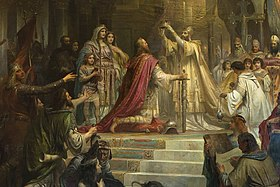
\includegraphics[scale=.5]{a20191225FromClovistoCharlemagne-img001.jpg} 
\end{wrapfigure}

\paragraph{Clovis (466-511)}
Clovis was the first of the 40 kings of France; he united all the Frankish tribes under one ruler. He was Baptized on Christmas Day 496, and three thousand of his companions converted with him.

\paragraph{King Ethelbert}
Pope Gregory the Great, having encountered some young Anglo-Saxons in a Roman slave market, was impressed by their beauty and blonde hair. He sent 40 Benedictine monks, under the leadership of Augustine of Canterbury (as he came to be known) to evangelize the English.

King Ethelbert embraced Christianity. Then he and 10 thousand citizens were baptized on Christmas day, year 597. The king’s baptism was the baptism of an entire people, who gladly followed their leader. From there, St Boniface and several monks set out to evangelize the Germans.

\paragraph{Charlemagne}
A century later, St Boniface was sent from England to evangelize the Germans. Progress was difficult, but after the felled the Donar Oak, without the gods subsequently striking him down, many pagans converted.

Charlemagne became King of the Franks in 768. As the Father of Europe, he re-united most of Roman Europe, even adding new lands to it. Charlemagne was not only a warrior, but the arts and sciences began to flourish again in Europe in the period called the Carolingian Renaissance. He valued learning and education. He encouraged the book publishing on a variety of topics, even founding a library at court. One of his favourite books was Augustine’s \emph{City of God}.

Charlemagne’s Coronation as Emperor of the Romans took place on Christmas day, 800 in Rome. The Roman people acclaimed:

\begin{quotex}
To Charles Augustus, crowned by God as great and pacific Emperor of the Romans, life and victory. 

\end{quotex}

Augustus was the same title claimed by Constantine, emphasizing the continuity between what was to be the Holy Roman Empire with the classical Roman Empire.

\flrightit{Posted on 2019-12-25 by Cologero}

\begin{center}* * *\end{center}

\begin{footnotesize}\begin{sffamily}

\texttt{Cologero on 2020-01-26 at 19:54 said: }

But the recovery of the Mediterranean West is prepared by the Empire of Charlemagne who, through a universal force characteristic of men who hold the spiritual and ethnic-blood heritage of the Romulean lineage, organizes Italy, France and part of Spain: it is strengthened with the supernationalist constitution of the Holy Roman Empire, continues its struggle through the maritime daring of the Maritime Republics of Genoa, Venice, Pisa and Amalfi. \flright{\textsc{Massimo Scaligero}, \textit{La Razza di Roma}}

\hfill
\end{sffamily}\end{footnotesize}

\section{Catching our Breath}

\begin{quotex}
The fool does more harm by his ignorance than the wicked man by his wickedness. \flright{\textsc{Al-Ghazali}}

\end{quotex}

It is time for a recap what has been accomplished thus far in our project to determine the lineament of the Western Tradition, which we claim is as real and as important as anything arising from the East. First of all, we outlined the features of the religion of the Ancient City, how the city was founded by a man-god, its cults, the importance of spiritual authority and its caste based social structure. We showed its decline due to the degeneration of castes which led to the decline of the ancient pagan civilizations due its forgetfulness of its own tradition.

We turned to the next stage of Western tradition, which was both an overthrowing of its decadent predecessor as well as being in continuity\footnote{\url{https://www.gornahoor.net/?p=3281}} with it; this is called Christendom. Ignoring the rather bizarre conspiracies that abound today, we rely instead on \textbf{Rene Guenon}'s sober and intellectually sounder understanding. Christianity at its inception was a mystery religion, founded by a man-god, just as were all the Greek and Roman mysteries and cities. You can accept this claim or not, it has no bearing on what follows. As it became the dominant religion, it was compelled to become exoteric as the social structures of the Roman Empire unraveled. However, we see maintained the outward characteristics of a traditional society: the distinction between spiritual authority and temporal power, as well as a caste based structure with a strong warrior caste\footnote{\url{https://www.gornahoor.net/?p=277}} with its own set of orders. Nevertheless, Guenon insisted on the esoteric character of the dominant spiritual tradition of Christendom, providing many examples from Gospel stories to \textbf{St. Bernard} to \textbf{Dante}, inter alios.

Next, we pointed to Ananda Cooomaraswamy\footnote{\url{https://www.gornahoor.net/?p=556}}, a man whose immense intellect bridged both East and West. He listed several Western authors whose depth of thought rivals that of the East. It would be risable, if it weren't so tragic, to see well meaning men turning to the East while remaining utterly ignorant of the great Western Traditional minds. Please read that piece over and over.

Even \textbf{Julius Evola} had to concede the Traditional nature of Christendom, as much as he disliked its dominant spiritual tradition. Yet, he did make the important point that it was the result of the collaboration of Roman and Nordic elements, the result of which was the spiritual unity of all of Europe, something which did not exist prior to the Middle Ages nor after it following the various reformations and revolutions. His claim that the best aspect of the Middle Ages was its pagan elements is like saying the best part of a cup of coffee is the sugar. They cannot be separated. Furthermore, the spiritual authority defines what it is, which is why Sola Scriptura needs to be rejected.

We then did a creative re-reading of several important figures of Christendom, understanding them as exponents of an esoteric tradition. This, I believe, was very fruitful and it needs to be extended and developed by others. That brings us to the next step which is Guenon's contention that the esoteric tradition has been totally lost in the West, or else it is deeply hidden. We pose the question somewhat differently. First of all, we deny that it has been lost as Tomberg and Mouravieff demonstrate. Whatever their defects may be, they absolutely show the continuing influence of Hermetism, at least in the East of the West. If you doubt the significance of that, please go back to that Coomaraswamy piece and then look up what the ancient Christians wrote regarding Hermes Trismegistus.

The second point is somewhat different. Now, the religion of the Ancient City is certainly lost, in the very real sense that it is unrecoverable — it was lost even at the time of the Roman Empire when men no longer understood their own traditions. The revival is this paganism requires a revelation from a man-god and can never be the result of an artificial reconstruction or re-enactment. On the other hand, the metaphysical teachings of Christendom have not been lost and they even have adherents today. What we can admit, instead, is that the teachings remain virtual, not actual. It would take a gnosis (not a conceptual understanding) to make them actual. However, since they are virtual and not genuinely lost, there remains the possibility of their being actualized. Thus, any objections to self-initiation are beside the point. Anyone confirmed by someone with valid orders has this understanding virtually; under the right circumstances, it can be made effective. We have recently provided examples of the Infinite\footnote{\url{https://www.gornahoor.net/?p=3261}} and the Intellectual Soul\footnote{\url{https://www.gornahoor.net/?p=3390}} which demonstrates beyond a doubt the understanding of the Middle Ages.

Now, we are about to turn to some modern thinkers to show the way from the virtual to the actual. \textbf{Vladimir Solovyov}, who represents the East of the West, was concerned in overcoming the breach between them. As Guenon points out, there is a relationship between theological and metaphysical language. Gornahoor has never engaged in religious polemics, which are pointless. However, Solovyov has developed a metaphysical system which is compatible with his theological understanding. What Guenon hinted at, Solovyov actually accomplished. That is why it is so important to anyone envisioning the religion of the future. Even those who foresee a return to some sort of paganism have to achieve the same level of metaphysical understanding.

\flrightit{Posted on 2011-11-20 by Cologero}
\section{Dante and the Holy Culmination of the Roman Tradition}

\begin{quotex}
From La Tradizione Romana by \textbf{Guido De Giorgio}. 

\end{quotex}
The traditional gold vein of Rome in the living unity of the two forms supplementing each other in a perfect match and equilibrium, is found again in all its wholeness in Dante who was the first to reveal the mystery of Romanity. The sacred arriving at the creative synthesis of the elements contained in the ancient and new traditions for which he can be called the prophet of Fascist Catholicity [Cattolicità Fascista] in the absolute meaning of the expression.

Poetry in him resumes its place and its sacred destination, it follows ``the footprints" as Boccaccio said, the traces ``of the Holy Spirit", it is no longer psychological and artificially descriptive, but an initiation, revelation, and realization. While theology is expository and proceeds discursively, submitting itself to the limits of reason illuminated by revelation, poetry grasps with supersensible intuition the mystery of the symbols and internalizes them, transforming them into shapes, living them, surpassing their representative exteriority so that to make of them the most suitable vehicle for liberation. In this sense, and in this sense only, Dante is the poet and the Comedy is the sacred poem, vehicle of the divine truth and supreme effort, the highest perhaps that was ever accomplished, to transform the sensible image the reason for the realization of traditional metaphysical principles, grasped in two directions, the ancient and the new, indissolubly unified in the occult name of Rome that is the seal of the divine song.

Thus, the universality of Dante was unique among men and poets, even though the anagogical interpretation of the Comedy had not yet been tried, in order to be completed and realized only ascetically by those who belong to the Race of the Spirit and who are the true key bearers of sacred science and the fasces bearers of divine power.

The Comedy is the supreme pilgrimage of the worlds considered as the only temple of God: if the point of departure is the earth and that of arrival is heaven, this apparent duality shows man only what he must reach when \emph{he is not what he is}, what he must become in order to be what he is, and how his earthly humanity is only a veil, when removed, the Divine Reality is revealed in His original unity, ineffability of the Ineffable. Only at this point poetry ceases and with the realization of the mystery of man who is the Reality of God, the Comedy finishes because the pilgrimage is completed, the end is reached, death is overcome, \emph{fieri} [becoming] became \emph{esse} [being] and \emph{esse} the radical non-existence of the Divine Night.



Heaven and earth are dissolved in the last smile of the Comedy, when the bright axe that dominates the Fasces [Fascio Littorio], resolving the enigma of the two-faced Janus through the plenary universality of the Cross, revealed the occult name of Rome and dissolved the Vestal fire on the lips of the Lord of the last rite. Here the mystery ends and the brilliant flashing ends in the essential tonality of the Silence, lord of Forms and Rhythms, the highest peak of integral realization. The ancient and new tradition led the poet to the secret of the Primordial Tradition, to the ``\textit{letizia che trascende ogni dolzore}" [``joy that transcends every sweetness of delight"]. In the paradisiacal vortex, it is completed and having completed itself it untied the traditional knot, nor can there be anything in what alone is it integrally and completely.

This is the miracle of the occult name of Rome and this is the reality of Dante and the Comedy.

The vision of the peak, insofar as it is so imperfect of the expression that tries to grasp its mystery, permits it to better consider the foundation and the progression and, what is more important to our task, the unification of the two traditions in Rome, i.e., in the Spirit of God. It is not possible to allude to this, unless metaphorically, in this simple introduction to the doctrine of the Roman Tradition, that cannot try to be more than what it is, a vestibule to the Temple, a preparation to the work of integral restoration of Traditional Romanity contained in the Comedy that is the sacred poem of Rome, no longer the ancient and new, but the eternal.

If Virgil represents the ancient tradition and Beatrice the new tradition and if, at the threshold of the Terrestrial Paradise, Virgil disappears before Beatrice, Beatrice also disappears when the divine mystery is grasped by Dante in its immediate realization and what then remains, above and beyond the two traditions unified forever is, climactically, Rome.

Virgil guides the poet through the world of Forms and Rhythms, in the two spheres of bodies and shadows, that he knows perfectly because he belongs to a tradition in which these two domains particularly were meticulously observed and studied, domains that constitute the subterranean and sublunar underworld whose secrets are fully treated in the three Virgilian works ``\textit{sotto il velame delli versi strani}" [``under the veil of strange verses"].


The ancient Roman tradition attached great importance to the knowledge of the immediate and psychic world governed by laws of internal, occult order, that embrace the totality of beings and things considered always with reference to the forces whose expression they are. The so called ``concreteness" of the Romans was based exactly on the precise meaning of these forces that act most visibly in the existence of man inserting there a hidden network of which the events, especially ``chance" events, as the common people believe, are the most significant effects: these forces are either propitiated, dominated, or determined. Virgil represents in the Comedy the knowledge of the two subterrestrial and superterrestrial worlds, the latter term however meant in the much more precise sense that must be given to the third element, the air, which symbolically corresponds to the subtle elements, the Rhythms, more through their ``diffusivity" than for their nature.

In hell, we are present at the extreme concretion of these unchained forces and, so to speak, precipitated in the closed vortex of ignorance, while in Purgatary, we catch sight of them liberated from the formal element in their spontaneous structure of the subtle body, the shadow. Virgil guides his disciple with ``art" up to the threshold of the Terrestrial Paradise from which ascent will begin at the paradisiacal levels, i.e., at the higher states that are forbidden to them because they realize only by means of Revealed Science, Beatrice.

Up to this point the two traditions remain separate even though the one is resolved in the other, that indicates Dante's dismay at Virgil's disappearance in the face of the vision of Beatrice. In the Terrestrial Paradise we have the explanation of the traditional integration, after the theory that leads the symbolic cart in front of the central tree which revives, discovering the reigns of the Silence where only the ascension to the divine states is accomplished. In other words, the second tradition is not opposed to but reveals the first, and completes it, bringing it back to the invisible centre from which everything emanates and to which everything returns as long as it is stripped bare to its original essence.

What in the first tradition is the \emph{Imperium} [empire], is the \emph{Regnum} [kingdom] in the second, while separately they indicate respectively temporal power and spiritual authority, there is an absolute seat in which while converging they merge into each other, and this seat, materially, symbolically, and actually is Rome. So that, while the second tradition illumines and reveals the first, the first precedes, prepares, and exists only for the affirmation of the second; there is an initial necessary opposition that is resolved only in Rome when, i.e., a unifying centre is found that is at the same time the neutral point where the traditional quarrel ends.

It is not easy to express this succession and fusion that must not be considered historically but on a plane where the symbolic values remain such even if unknown or misunderstood until a new light suddenly illuminates them and reveals them. For the two traditions which we discussing, Rome is this light and the Comedy is the poem of sovereign and Holy Rome, the unifier, while Fascism is the operator of the synthesis in which the two forms are compounded in a new revelation of power. The greatness of Dante consists in the statement of these two aspects, the ancient and the new form, of the same tradition that is Roman universality, and, while in De Monarchia he combats, as he says, \emph{pro salute veritatis} [``I engage in battle in this book for the cause of truth"] to reclaim the ancient tradition that had to remain to sustain the second. In the Comedy he arrives at the realization of the unification, at what we will have to call traditional perpetuity, showing the reality of a transhumanization [passage from a human state to a superhuman state] in all its levels that embrace beings and elements, world and afterworld [\emph{soprammondo}], heaven and earth, from Forms to the Rhythms in the Silence.

He is therefore the advocate of Sacred Science in the living, and not theoretical, wholeness of the Roman Tradition, of the \emph{Imperium} and the \emph{Regnum}: the ancient and new traditions mutually sustain each other, avoiding thereby all incongruity of a conflict that would impoverish them, impeding their supreme synthesis which is, practically, the equilibirum of the temporal and the spiritual and, at the centre of realization, the complete transfigurative process, the integral initiation, the real ascent from the earth to the elementary and trans-elementary heaven.



All the symbols of the ancient tradition live again in the creative light of the achievement, the union with god [\emph{indiamento}], and the Argonautic enterprise finds its fulfillment in the revelation of the true face of God with which the last canto and the last canto of the ``Sacred Poem" end. The vein of gold, the vestment of glory, is dressed by Dante in the great light of Rome, highest peak in the radiant circularity of the Ineffable. All the traditional sciences flow together in the Comedy through a dynamic complexity of states and a perfect knowledge of the transitions in the ambit of the three worlds through which the process of the cosmic-human illusion takes place, up to its resolution in the supreme principle in the three phases corresponding to the death, resurrection and transfiguration of man in God. The process of death is slow, gradual, and it embraces all terrestrial experience in its most interior forms to which the vices correspond in the moral sphere, i.e., animality: from here, the \emph{descending} hierarchy of the underworld where the realizing interiority assumes over itself all human development reducing it to a totalizing unity of life integrated in the being that had and lost the light, Lucifer. He represents the maximum concretion in the scheme of diabolic unity, the inverse reflection of the divine unity of which he has only the Trinitarian analogy in the three faces that are turned antithetically while in God they are homocentric and confluent.

Human plurality is resolved in its huge body, congealing itself, solidifying itself, petrifying itself: he represents the fall, the precipitation, the last terrestrial coagulation of the impassable waters, the freeze, the totalization of ignorance and darkness: its night corresponds, according to the reverse analogy, to the night of God, to the precreative indistinction in which all the determinations of being are based, as in him all the determinations of non-being, i.e., of evil. The analogy is perfect even in that Lucifer is the first and the last as God is the alpha and omega, but while in the first case, one has a duality of movement represented by the fall, in the second instead we have the essential unity of the opposites considered as the two confluent points of the divine cycle. Lucifer who \emph{was} the first \emph{is} the now the last: in him the temporal cycle is resolved in the eternity of evil, as in God the eternity of good is resolved. The two main antitheses represent what can be called the highest \emph{critical polarity}, i.e., the terrifying point of active realization, that precisely in which Virgil very painfully creates the \emph{overthrowing} which is a \emph{rectification} where the descendant interiority becomes the ascendant interiority and the place of damnation, the basis of salvation. From the stony precipitation whose symbol is Lucifer the ascendant rectification begins and the stone that is concretion and fall becomes the basis necessary for the flight toward the elementary complexity and the trans-elementary totality.

Purgatory is the place of the second birth from Forms to Rhythms in a hierarchical purification of which the seven terraces [of the mountain of Purgatory] are pointers: it is not a passage from Forms to Rhythms but a resolution of Forms in Rhythms, of the body in the shadow, of corporeity in psychicity where then even this is freed in the spirituality that is the Silence, Paradise. Virgil's ``art" is the perfect knowledge of the two spheres, the Forms and the Rhythms, through which the decoupling from error and from the ignorance of human and terrestrial fallacy is accomplished hierarchically, since reality is one, that of God, but a man has knowledge of this reality only when he integrates it, realizes it, becomes it. Up to what is not completed, it is necessary to traverse the levels of development that, from the human point of view, are the three corresponding to Hell, Purgatory, and Paradise. Dante in the Comedy proposes and exposes all the experience of realization, the complete, integral initiation, through positive knowledge, lived in all the levels that lead from the human to the divine. In the two first kingdoms, the ancient tradition sufficed to lead this path to completion and Virgil represents the science and the knowledge of the laws that govern the subterrestrial and sublunar world. He disappears before Beatrice because he dissolves in her, is completed in her, not because he opposes her as would be the case if Dante had considered the two traditions irremediably different and antagonistic as everyone believes, as much by those who exalt the first as by those who oppose the second. Beatrice appears at the moment when the first guide, Virgil, has completed his work and embraces the gross and subtle manifestations, the Forms and Rhythms. The exercise of human reason in its complete and normal development naturally leads to the sphere where a process of mystical union with God [indiamento] is initiated in the levels of the non-formal, i.e., in the zone of the Silence represented symbolically by the heavens.

Here Sacred Science, Beatrice, carries out the integrative cycles of unity in a flight that is light and salient flame between the Rhythms circularly untying itself in the plenitude of the Divine Being. The Trinitarian scheme is amplified in the assumption of the nine hierarchies, effulgent wings that facet the divine infinity of the joyful love of the Angels, Archangels, Principalities, Powers, Virtues, Dominations, Thrones, Cherubim, Seraphim, where celestiality is engraved in relations of light and splendour in the face of the terrestriality which is overcome, resolved, and dissolved in the divine whirlpool. There still remains, in the first seven heavens, the divisibility of the light with planetary vertices in a progressive self-realization of perfection in unity, a display of radiations in the body of the divine diamond.

In the residence of the sun where the zodiacal band combines with its perfection of the ternary and quaternary resolved in the supreme syntheses of the trinity ($12 = 1 + 2 = 3$), the mystery of the Perfect Man, the Triumphant Christ emerges, the perfection of the divine sonship in absolute assumption of radiance. It comes after the last creative level of the ninth heaven of the Trinitarian perfection, assuming in each of the Divine Persons the seal of the others so to project the mystery of the Ineffable in the creative circularity, then finally the absolute level, the culmination perpetuating itself in the eternal scheme of the worlds, the Empyrean. Here Beatrice disappears, not like Virgil, to permit a progress, an arriving, an end, but to unravel the mystery of the Last Seal where the virginal matrix carries out the cyclic reduction of the light in the very face of God. The last level of Silence is integrated in the same riverbed of the Divine Night where the pulse of the Ineffable vibrates in the realizing unity of God, the Supreme Zero, transcendence of the plenitude itself, darkness of the Ineffable.

The purely exterior literary merits that common men [\emph{volgo}], the \emph{profanum vulgus} [unholy rabble], admire in Dante have no importance and would nullify the value of the Comedy in the very eyes of Dante and of those who can and know how to understand the purpose for which the poem was composed.

It would be necessary to feel ashamed to still speak of, and only of, ``art", ``poetry", ``brilliant construction", in the modern sense of the word when one alludes to Dante's work which is only and eminently sacred in spirit and structure, while the allusions to historical persons are clearly motivated by Cacciaguida at the end of canto XVII of the Paradise. But these allusions hide well dramas other than those that the profane see in it. Regarding these, the central motive, the general orientation, are understood, traditionally speaking, but it is not, nor perhaps will ever be, possible to explain entirely due to the impossibility of retracing the elements of a tradition that, in Dante's time, was entirely oral. As to the strength and the expressive completeness so steadfast in Dante, it is due to the very substance of the topics treated: it is about \emph{poetry of inspiration} in the absolutely sacred meaning of the word and those who know what is meant by such an expression, know the imbued power of the realizing wave that moulds the word in a type of revealing plasma where the specular miracle of the perfect reflection is accomplished. The same Rhythm, the homophony is adequate to the state that tries to be expressed in a way to constitute as many \emph{topoi} or static forms, normative traces in which the transfiguring synthesis from the image to the idea is completed, to substitute for the oral initiatic transmission.



The moderns, therefore, who for centuries have read, studied, and commented on Dante resign themselves to understand nothing of it as long as they persist in not considering him as a prophet, a sacred poet, whose work is the highest expression, perhaps unique, in the Roman Tradition, an eternally new synthesis of the two traditional forms that in Rome, in its occult name, will find their completeness and their perfection. Here is his greatness and his true originality: if the expression reaches a plastic and vibratory perfection never before equaled, that is due to the sacred character of the Poetry which catches the eternal light of revelation in the transience of phantasms and concentrates it in radiant syntheses. In Dante, East and West are balanced in a unique centre that, substantially, is the Primordial Tradition, i.e., the unique most important traditional universality and ultimate realization. Never during the Middle Ages were the relationships between East and West so close: never in those great centuries had the traditional elements completed each other and disclosed each other for oral transmission, direct from master to disciple and from disciple to disciple. Dante appears exactly at the end of this era but in a period in which Dominicans and Franciscans, although already degenerate and hostile, had outlined the two greatest ways of realization of the divine—cherubic and seraphic—homocentric even if divergent by nature and process. He unites these two ways substantially, bundles [fascifica] them without confusing them. And it is necessary to note that when we use the term \emph{fascificare}, we mean nothing that can be considered, even if only vaguely, syncretism or mixture: to bundle in the pure traditional sense means to give to each way, to each element, a unique direction, a centre, an axis without confusing them: this is the novelty of the traditional steadiness.

There is one bond that captures the twelve rods of the Fascist bundle [Fascio Littorio] and there is one lightening power expressed by the double cut axe: the emblem is traditionally the greatest because it represents the confluence in the vertical direction, i.e., that of elevation and conquest. In Dante fascification is supreme, East and West, ancient and new Rome, temporal and spiritual, heaven and earth, world and afterworld, man and God, everything gets becomes more marked, matches up, is unified at a supreme vertex that is Rome. This is Sacred Fascism, the true triumph of justice and truth in man and in the world: if there are quarrels, battles, falls, these have no importance since they take place in the bosom of a traditional society where everything is formed from the supreme balance assured by key bearers and fasces bearers, by the \emph{Regnum} and the \emph{Imperium} forever unified in Rome.

This is the perpetual peace, the universal peace which Dante constantly mentions in De Monarchia and in the Comedy: the reaching of the traditional equilibrium that can only contain and annul in a higher place of harmony the battles and the inevitable disputes in the world, where, since duality reigns, it is not possible to avoid conflict without which the supreme unifying element of Rome would be suppressed. But instead, when this element is restored to its true function and reestablished the bases of the Roman Tradition in their living integrity, a new greatness would rise from under the present ruins of the western world, a new purity of life and thought and the Temple protected by the sword would rise up in the light of Rome for the glory of God in the heavens and the peace of men on earth.


\hfill



\flrightit{Posted on 2012-03-21 by Cologero }

\begin{center}* * *\end{center}

\begin{footnotesize}\begin{sffamily}



\texttt{Matt on 2012-03-22 at 21:05 said: }

Cologero, your hunch (more aptly, intuition) about Fr. Johnson was correct.

Here's Johnson's relatively new podcast on Guenon.

\url{http://reasonradionetwork.com/20120315/the-orthodox-nationalist-rene-guenon}


\hfill

\texttt{Boreas on 2012-03-23 at 12:36 said: }

This text is like poetry in itself. A world of light and life eternal opened before my mind's eye when reading this. Beautiful, thank you.

``Night is preferable to a day."


\hfill

\texttt{Cologero on 2012-03-26 at 08:48 said: }

Apart from the annoying mispronunciation of ``Guenon", this lecture was more about Fr. Johnson than Rene Guenon. It addressed a small, albeit important, aspect of Guenon's oeuvre. A minor point: pace Fr. Johnson, Guenon did indeed make a distinction between Eastern ``religions", such as Buddhism, and Western (so-called Semitic) religions.


\hfill

\texttt{Cologero on 2012-03-28 at 12:36 said: }

Here we see de Giorgio as the reconciling force of the Western Tradition, finding unity and harmony where others can only see difference and conflict. Unlike contemporary men who read into the past their present experiences, this is how the Medievals saw themselves. Like the ancients, the medievals had their High Priest and Emperor in Rome; despite the differences in outward form, their was a continuity in their inner life. Dante is, therefore, the holy culmination, the prophet, the revealer of that continuity.

Poetry in Dante is has nothing to do with the psychological fantasies of the moderns; rather, for him, it is a revelation of the Holy Spirit, the way of initiation, with the goal of realization. The symbolism of the Comedy is intractable to the rational mind and is comprehensible only to those with a developed spiritual intuition.

The Comedy describes a pilgrimage, or a quest, from the three worlds, analogous to those of the Tao. When the path is traversed, death is overcome, becoming becomes being in the Divine Night.

When de Giorgio writes of Fascism, he is not just referring to a limited political movement in Italy of the 30s, but rather to the Roman Tradition, which was the ultimate source of the symbol of the Fasces\footnote{\url{http://upload.wikimedia.org/wikipedia/commons/thumb/7/74/Fasces_lictoriae.svg/224px-Fasces_lictoriae.svg.png}}.

The Comedy leads us to the Primordial Tradition, which has a joy that transcends any little delights we may experience in our ordinary life. The path leads from earth to heaven. Nietzsche exhorts us to ``become what you are". But it requires a Dante to tell us who we are and how we can become it.


\hfill

\texttt{Matt on 2012-03-28 at 17:14 said: }

These translations of de Giorgio have been great. Are you thinking of translating anymore? His approach to Tradition I must say is rather fascinating (and from the description of him in Evola's Path of Cinnabar, de Giorgio the man is fascinating).


\hfill

\texttt{Matt on 2012-03-28 at 17:15 said: }

Never mind, just read one of your earlier comments that states you will provide more. Apologies.


\hfill

\texttt{Cologero on 2012-03-28 at 19:02 said: }

The way to encourage us to provide more translations, which, obviously, we do not require for ourselves, is to engage in a lively discussion in the comments. Readership has gone down in each of the four installments, so, unfortunately, not everyone shares your enthusiasm.


\hfill

\texttt{Cologero on 2012-04-05 at 07:45 said: }

The occult, or secret, name of Rome is an idea that may be unfamiliar to some readers. Besides its public name, Rome had a secret name that was only used in certain rites and rituals. Only the High Priest and his associates even knew that name. Presumably, this secret name has long been forgotten. Some say it is Amor (Roma spelled backwards), which means Love.


\hfill

\texttt{Cologero on 2012-03-28 at 13:08 said: }

``Shadow" here needs to be understood in the sense of shade, or ghost, as the ancients understood the post-mortem state in the afterworld. Vigil leads Dante through the worlds of gross and subtle manifestation (forms and rhythms). These worlds were well understood by the ancients, as Virgil wrote of them in his own inspired poetic works.

The ancient Romans knew the occult forces behind those worlds, which they either propitiated in their rites or learned to dominate. The third dimension of depth, these occult forces, elude the minds of the vulgar, both in the past and even more so in the present.

Hell, then, is the most concrete form of gross manifestation, and Virgil shows the way to subtle manifestation. However, he yields to Beatrice who brings Dante to the threshold of understanding non-formal manifestation. Most men, because they either adhere to the ancients or the medievals, can see only a division and a separation. However, Dante reveals that this division is illusory.

De Giorgio's view is quite different from that of Duke di Cesaro, who regards the ancient (and eventually even the medieval) tradition as something to be overcome and discarded in some evolutionary master plan. No, de Giorgio shows that the ancient tradition is fully revealed and completed in the medieval tradition, which itself would be partial and incomplete without the earlier.

The each have their role in the synthesis. The ancient tradition is the Empire, or temporal power. This is where Evola stops and it colours his understanding of the Medieval synthesis. The medieval tradition is the Kingdom of God, representing spiritual authority. Both wings of the eagle are necessary, and this is the meaning of the symbol of the two-faced Janus\footnote{\url{http://en.wikipedia.org/wiki/Janus}}. Rome is the centre, and the quarrel between the two traditions must end, once this is understood.


\hfill

\texttt{Matt on 2012-03-28 at 17:20 said: }

``Shadow" here needs to be understood in the sense of shade, or ghost"

Kind of like a psychic corpse?


\hfill

\texttt{Cologero on 2012-03-28 at 19:14 said: }

I'm afraid, Matt, that I cannot provide every reference for every conceivable topic, as much as I try. Since Virgil did include ghost stories, it would be nice if readers can fill in the gaps … you cannot continue to expect George to do everything for you.

For those interested, a place to start is this painting by Ary Scheffer\footnote{\url{http://en.wikipedia.org/wiki/File:1855_Ary_Scheffer_-_The_Ghosts_of_Paolo_and_Francesca_Appear_to_Dante_and_Virgil.jpg}}.


\hfill

\texttt{Matt on 2012-03-28 at 19:48 said: }

The question was rather redundant in hindsight.


\hfill

\texttt{Cologero on 2012-03-31 at 12:58 said: }

We see in this segment that de Giorgio is confirming Guenon's teaching on symbols. He write: ``symbolic values remain such even if unknown or misunderstood until a new light suddenly illuminates them and reveals them." The symbol is there, even if its full meaning is hidden, or occult. Dante reveals in the Comedy the meaning of the occult name of Rome.

He prepared the way in De Monarchia in which he revealed the full meaning of and justification for the first Rome. The way from a human state to a transhuman state is revealed in the Comedy. This is understood by very few today, and I suspect this is the first exposure of this occult teaching to most if not all Goranhoor readers.

Those who cannot move beyond the first Rome of the Imperium are unable to progress. Those who don't understand the second Rome of the Kingdom have lost touch with their own Tradition. Clearly we mean here a living connection, as de Giorgio writes, not merely a theoretical understanding.

``Indiamento" is the word used in neo-Platonism for the mystical union with God. Once again, de Giorgio is making clear this connection, at least for those who make the effort to see and are not blinded by their pre-existing prejudices.

The nine hierarchies, which we have described in \textit{Spiritual Beings}\footnote{\url{http://www.gornahoor.net/?p=1941}} can be understood as semi-divine beings or as higher, transhuman states. A fascinating metaphor used by de Giorgio refers to them as ``facets". In other words, the ``Trinitarian scheme" is passed through, as it were, the facets of a diamond, and like a prism, separate the divine Light into the multiplicity of the world. Hence, the angelic hierarchies assist in the creation (or emanation) of the world.

It is worth meditating on the idea of the Perfect Man, that is, the man who realizes all his possibilities as both Guenon and Evola have written about. The end of such a meditation will be the realization of the Absolute Being; but the way to such a realization is only through the Perfect Man.


\hfill

\texttt{Cologero on 2012-04-01 at 13:01 said: }

Like his colleague Rene Guenon, Guido de Giorgio regards the Divine Comedy as an inspired work describing a spiritual path. Vulgar minds, and de Giorgio would include academics in this category, fail to grasp this aspect of the Comedy. Some even see in the Comedy, nothing but racism, anti-semitism, and homophobia\footnote{\url{http://takimag.com/article/the_divine_comedy_funnier_than_ever_taki_theodoracopulos/print\#axzz1qoAHKtSq}}. The many allusions to events in Florence of some 8 centuries ago hide deeper meanings that are lost on them.

Dante rectifies the division between the East and West, as his goal is the Primordial Tradition. The references to the Dominicans and the Franciscans represent two competing spiritual styles. They can be understood as the difference between Apollonian and Dionysian initiations.

Given the human situation, men continue to fight illusory battles: between Apollo and Dionysus, pagan and christian, east and west. At a higher level, these views are unified. When this becomes understood by all the parties, then the Western World will return to its previous vigour.


\hfill

\texttt{Cologero on 2012-04-06 at 11:29 said: }

Why did Dante place Plato and the Philosophers in hell?

Some readers may remember Exit, who until now has honored a voluntary ban on commenting here. However, he did ask a pertinent question about the Comedy. On the assumption his question was sincere, I decided to pass the question on. Perhaps some readers are willing and able to respond to it, keeping in mind all that we have written on the topic, following Guenon and Guido de Giorgio.


\hfill

\texttt{apeiron on 2012-04-06 at 16:08 said: }

While the paganism of antiquity could interpret the divine, it only went half-way and this is discounting the prejudices of catholic dogmatism. Discursive thought is not unifying logos. That is the problem with philosophy. No matter how close the articulations are to the primordial (exempli gratia, Heraclitus) it begins the rationalist discursive cycle after the initial divine act has lost its potency. There is more power in the act.


\hfill

\texttt{Cologero on 2012-04-06 at 22:35 said: }

Thanks, apeiron, for the intriguing comment, but that did not please the questioner. Unfortunately, the vulgar can interpret the Comedy as a travelogue, rather than as a description of states of consciousness on the path to the primordial state.

To clarify a point, the pagan philosophers and poets inhabit Limbo, just outside of Hell. There is no suffering per se (other than, perhaps, the loss of hope). They live in the natural light of reason and a natural happiness. Their post-mortem state is not a negative judgment of Dante, who greatly respects those poets and philosophers. Rather it is a matter of justice, since that is how the pagans themselves envisioned the afterlife. We alluded to this when we mentioned Virgil's description of ghosts or shadows, from Aneas' descent to the underworld.

In an upcoming post, we will deal with Evola's description of the afterlife. While we respect Evola, this will show his limitations since he also cannot conceive of higher states. Evola did not know the occult name of Rome.


\end{sffamily}\end{footnotesize}


%En The Owl of Minerva, sigue con tres tipos de hombres: Vidente, héroe y creyente. ¿Un capítulo para cada uno en tipos de caminos espirituales?
%Valores familiares, sociales
%Mundo moderno

\chapter{Monarchy}
\section{The Meaning and Function of Monarchy}

\label{sec:MeaningMonarchy}

\begin{quotex}
This essay by \textbf{Julius Evola} was published under the title \textit{Significato e funzione della monarchia}. It was included in ``La monarchia nello Stato modern" by Karl Loewenstein, 1969.
\end{quotex}

\paragraph{Monarchy as a Possibility Nowadays} K. Loewenstein's essay has provided the reader with an overview of all the various forms of monarchy and the possibilities that, in his opinion, remain for a monarchical regime in the present age. Monarchy, as we have seen, is not taken in the literal sense of the term (government of one man, power concentrated in one man) but, correctly, in its traditional and most current sense, i.e., with reference to a King.

Loewenstein's conclusions are rather pessimistic. In order to exist in our day, monarchy should resign itself to being a shadow of what it had been. It could be conceived only within a democratic framework and, properly speaking, in the form of a parliamentary constitutional monarchy. Apart from England, which would be a special case, the model offered by the monarchies of the small states of northern and western Europe — Sweden, Norway, Denmark, Belgium, Holland, Luxembourg — is what should possibly be kept in mind.

In the analysis of the range of the various arguments adopted in favor of monarchy, Loewenstein tried to be objective, but was unable always to be so. The precise aversion to every principle of true authority is quite visible in him, while an insufficient emphasis is given to the factors of an ethical and immaterial character. Now we believe that if you were forced to conceive of a monarchy only in an empty and democratized form, besides only being possible because it concerns marginal small states, not yet involved in the dynamism of the great forces of the era, we undoubtedly might as well end the discussion in the negative.

It must be recognized, however, that pessimistic conclusions regarding monarchy appear largely justified only if you hypostatize the situation of the current world and believe that it is irreversible and destined to continue itself indefinitely. This situation is defined by a general materialism, the prevalence of base interests, the egalitarian error, the government of the masses, technocracy, and the so-called ``consumer society." Except that we are beginning to multiply the signs of a profound crisis of this world of affluence and counterfeit order. Various forms of revolt are already noticeable, for which it is not impossible that it could reach a state of tension and a breaking point, and that, especially in the face of possible liminal situations, tomorrow different forms of sensitivity may be reawakened, reactions occurring similar to those an organism is capable of when it is mortally threatened in its deepest being.

The supplanting, or to a lesser extent, of this new climate is the decisive element also for the problem of monarchy. In our opinion, it should be placed in the following terms: What meaning could monarchy have in the case that such a change in climate should take place, and in what form could it be a center for the reconstitution of a ``normal" order — normal in a higher sense? Certainly, the presence of a true monarchy in a nation would have a rectifying power, but this is a vicious circle: without the premise that we mentioned, any restoration would have a contingent, not organic and, in a sense, unnatural character.

The disorder present in the political field, everything that it shows of instability, dangerously open to subversion — to Marxism and communism — substantially derives from the deficiency of a superior principle of authority and from an almost hysterical impatience for such a principle, through which certain political experiences of recent times serve at most as a convenient alibi. Speaking of a superior principle of authority, we refer to an authority that has an actual legitimacy and, in a certain way, a ``transcendent" character, because without this, authority would lack any basis, it would be contingent and revocable. A truly stable center would be missing.

It is important to clearly fix this essential point, in order to differentiate the type of monarchy, which this essay deals with, from monarchy in the broad sense of power or government of one man. In fact, spurious counterfeit forms of authority are conceivable, and are even realized. Communist regimes are also based on a de facto authoritarianism that can disguise the crudest and even tyrannical forms which are the justifications that they mendaciously give. One can put the dictatorial phenomenon along the same lines if it is conceived otherwise than in relation to emergency situations as originally occurred in ancient Rome.

On the other hand, the antithesis, so often advanced between dictatorship and democracy, is relative, except that you examine the existential foundation of these two political phenomena, that is, a ``state of the masses". If the dictatorship has not purely functional and technical characteristics (an example is offered currently by the Salazar regime in Portugal), if it is based on pathos as in some recent plebiscitary and populist forms, the same element galvanizing it is activated by every democratic demagoguery. The dictator makes a bad surrogate to the monarch with the appeal to forces that confusingly seek a foothold, a center, whatever it is, just to come to the head of chaos, disorder, situations that have become unbearable. This also explains, however, the phenomenon of possible, abrupt changes in polarity as a result of some trauma that has suspended the cohesive and driving force of the system, as in a magnetic field when the power goes out. The most perspicuous case is perhaps provided, in this respect, by the astonishing change in the collective political climate occurring in present-day Germany, after the almost frantic mass enthusiasm that had characterized the previous dictatorial period. It is significant that, on the contrary, a similar phenomenon of inversion was not produced in Germany after the First World War, because its antecedent was not a dictatorship but a traditional monarchy.

Through the ``transcendence" of the principle of authority characteristic of regality, the monarchical regime constitutes the only real antithesis both to dictatorship as well as absolute democracy. We must indicate the basis of its superior right for that reason. The various forms that it may take and the ideas or symbols that can legitimize this transcendence according to the times, do not touch the essential: the essential thing is the principle. Loewenstein is right when he says that in a world desacralized by the natural sciences, in which religion itself is undermined, there can no longer be a question of the mystique of the monarchy that in other times was supported on specific theological conceptions and a liturgy. But if you take a look at the world of the holders of the crown at all times and in all places, the recognition of the need for a stable center can be seen as a common and constant theme, a pole, something that to be truly stable must have, in a certain way, its own principle in itself or from above, which must not have a derived character. In this respect one can take a look, for example, at F. Wolff-Windegg's excellent work, Die Gekrönten. Someone rightly wrote: ``A purely political royalty — it can certainly be said — has never existed." Not so long ago, the sovereignty of divine right ``by the grace of God," did not imply, in its subjects, specific theological considerations; its value, so to speak, in existential terms, corresponded precisely to the need for a higher point of reference that absolutely does not happen when the king is such only through the ``will of the nation" or ``the people." On the other hand, only under that assumption could those dispositions, those forms of behavior and customs of a higher ethical value develop, in the subjects, in the sign of loyalty, which we will discuss shortly.

So we cannot share Loewenstein's opinion that the ideal argument in favor of monarchy is now invalidated. What he says is true, of course, namely that the decline of monarchy is due not so much to democracy as to the coming of cars and aircraft, the automobile, television — you can say, in general, the technological industrial civilization. But here we have to wonder if, in fact, we are entitled to hypostatize this civilization, we must ask ourselves to what extent man wants to accord to everything a value different from that of a set of simple, mundane means, which in ``consumer society" leaves an absolute inner emptiness. Let us repeat: it is primarily a question of the ``dignity" of monarchy, an esteem and a right that always and everywhere drew from a supra-individual and spiritual sphere: sacred investiture, divine right, mystical or legendary filiations and genealogies, and so on, were only imagined forms in order to express an always recognized substantial fact, namely that a political order, a truly organic and living collective unity is only made possible where there is a stable center and an elevated principle in respect to any particular interest and the purely ``physical" aspect of society, a principle independently having a corresponding intangible and legitimate authority. Therefore, in principle what Hans Blüher wrote is absolutely correct: ``A king who lets his sovereign function be confirmed by the people, admitting thereby that he is accountable to the people — instead of being responsible for the people before God — such a king renounced his kingship. No infamy committed by a king — and God knows if they were not committed — destroys the mystical objective sanction of the sovereign. But a democratic election destroys it immediately."

\paragraph{The bound of loyalty} If in the past, the bond of fidelity that united the subject and follower with the sovereign could be treated as a sacrament — sacramentum fidelitatis — something that was preserved even later as the quite perceptible foundation of a special ethics, an ethic, in fact, of loyalty and honor, which could acquire a particular force in the assumption, just now indicated, of the presence of a personalized symbol. In normal times, the fact that the sovereign as an individual might not always be at the height of the principle, did not matter; his function remained unprescriptive and intangible because obedience was not to the man but to the king and his person had value essentially as a support so that the capacity for super-individual dedication, that pride in serving freely and possibly even the readiness to sacrifice (as in the dramatic moments when a whole people rallied around their sovereign) could be awakened or propitiated, that they might constitute a way of elevation and dignification for the individual and, at the same time, the most powerful force to hold together the union of a political body and to limit in it what it has that is anodyne and disheartened, and in recent times has taken a dangerous extent.

That everything that cannot be achieved to the same extent in another form of political regiment, is quite obvious. A president of the republic can be flattered, but no one will ever recognize in him anything but a functionary, a ``bourgeois" like any other, which only extrinsically, not on the basis of an inherent legitimacy, is vested with a temporary and conditioned authority. Whoever maintains a certain subtle sensibility perceives that ``being in the service of their king", the ``fight for their king" (even the fight ``for their own country," despite the romantic coloring, has in comparison something less noble, more naturalistic and collectivistic), the ``representing the king", all have a specific quality, all of which indicates instead a parodic, not to say grotesque, character when it pertains ``to one's own president". Especially in the case of the army, high bureaucracy, and diplomacy (regardless of the nobility), this appears very obvious. The same oath, when it is not paid to a sovereign but to the republic or one or another abstraction, has something discordant and empty about it. With a democratic republic, something immaterial, but still essential and irreplaceable, is inevitably lost. The anodyne and the profane prevail. A monarchist nation that becomes a republic is, in a certain way, a ``degraded" nation

If we observed that the kind of fluidity that forms around the symbol of the Crown is quite different from what may be related to the exalted ``states of the multitude", which can arouse or favor the demagogy of a popular leader, the difference also exists with regard to any simple nationalistic mysticism. Of course, the sovereign also incarnates the nation, symbolizes its unity on a higher plane, establishing almost, with it, a ``unity of destiny." But here we find the opposite of every Jacobin patriotism; there are none of those confused collectivizing myths that speak to the pure demos and that almost divinize it. It can be said that monarchy moderates, limits, and purifies simple nationalism; which, as it prevents any dictatorship replacing it with advantage, so it also prevents any nationalistic excess; it defends a structured, hierarchical, and balanced order. It is known that the most calamitous upheavals of recent times can be attributed mainly to unrestrained nationalism.

After what we have said, it is clear that we do not share at all the idea that monarchy at this point should be democratized, that the monarch should assume almost bourgeois features — ``must come down from the august heights of the past and present himself and act in a democratic way," as Loewenstein claimed. That would simply destroy his dignity and his raison d'.tre, as we indicated. The king of the north European countries who carries a valise, who goes shopping in the stores, who consents to letting radio or television display his well-behaved family life to the people including his tantrum-throwing children, or else the Royal House that is provided for the curiosity and gossip of the news magazines, and whatever else one thinks, might make people close to the king, including, in the end, a good-natured paternal appearance (if the father is conceived in a bland bourgeois form), all this cannot avoid damaging the very essence of the monarchy. The ``Majesty" then really becomes an empty epithet of the ceremony. It has rightly been said that ``the powerful who, through a badly understood sense of popularity, consents to get closer, ends up in a bad way."

It is clear that take to take all that as firm, means going against the current. But, again, we pose an alternative: it is a question of accepting, or not, a state of fact as irreversible, thinking that only the useless vestiges of monarchy can exist. One of the elements to consider in this regard is the intolerance in our world, for distance. The success of dictatorships and other spurious political forms is due, in part, precisely to the fact that the leader is seen as ``one of us", the ``Great Comrade," and only in these terms is he accepted as a guide and obeyed. In these circumstances the concern for `popularity' and for ``democratic" means is quite understandable. But that, basically, is anything but natural; we do not see why he should be subordinated when the leader, in the end, is just ``one of us" when an essential distance is felt, as in the case of the true sovereign. So a ``pathos of distance" — to use one of Nietzsche's expressions — should be substituted for that of affinity, in relationships that exclude any haughty arrogance on the one hand, and every servility on the other. This is a basic point, in its existential character, for a restoration of the monarchy. Without exhuming anachronistic forms, instead of propaganda that ``humanizes" the sovereign in order to captivate the masses, almost on the same line as the U.S. presidential election propaganda, one should see to what extent traits of a figure characterized by some innate superiority and dignity can have a profound activity in a suitable context. A kind of asceticism and liturgy of power could play a part here. While just these traits will enhance the prestige of the one who embodies a symbol, they should be able to exert a force of attraction on common man, even pride, in the subject. Moreover, even in fairly recent times there has been the example of Emperor Franz Joseph who, while interposing the strict ancient ceremonial between himself and his subjects, while not imitating in the least the ``democratic" kings of the small Nordic States, enjoyed a particular, not common popularity.

To sum up, the main prerequisite for a revival of monarchy, pursuant to the dignity and function which we mentioned, there remains, in our opinion, the awakening of a new sensibility for an order that is detached from the most material, and also the simply ``social", plane, and tends to everything that is honor, loyalty, and responsibility, because similar values in the monarchy have their natural center of gravity; while, in turn, the monarchy will end up degraded, reduced to a simple formal and decorative survival when these values are not alive and active — first in an elite, then in a real ruling class. They are not the same chords that the defender of the monarchical idea and of any other system must make resonate in the individual and in the community. So it is absurd to entrust the destinies of the monarchical idea to propaganda and a praxis that approximately copies the methods of the opposed party in a democratic spirit. Even today being able to ascertain the appearance of tendencies toward an authoritarian center, towards a ``monarchy" in the literal sense (= monocracy) is not enough, after what we said about the profound differences which the various objectifications of the principle of unity and authority may present. The meaning of what is not allowed to be sold, bought, or usurped in the dignity and participation in political life is a decisive factor and escapes like water through their fingers for those who think only in terms of matter, of personal advantage, hedonism, functionality, and rationality. If one must no longer speak of that meaning because of the famous Marxist ``meaning of history", which is claimed to be irrevocable, we might as well set aside definitively the cause of monarchy. This would, moreover, be tantamount to profess the most bleak pessimism in regard to what still can appeal to man of recent times.

\paragraph{Constitutional Monarchy}
After having considered the spiritual aspect of the problem of monarchy, it is necessary to indicate the aspects that are related on the positive, institutional, and constitutional plane. On such a plane, it will be necessary to make clear the specific function to attribute to monarchy and what differentiates a monarchical system from other systems. It is amazing that a comparable problem is almost not faced by the propaganda of the monarchists. In elections there were, even in Italy, discourses by the monarchists who blamed, more or less on the same lines of other sectors of the opposition, the dysfunctions of the republican democratic and partocratic State and the danger of communism, avoiding however indicating, in no uncertain terms and without fear, in which terms the presence of the monarchy would positively eliminate both, or, better put, in virtue of which particular prerogatives the monarchy would be for so much.

If one is really a monarchist, one cannot concede that the monarchy becomes reduced to a simple decorative and representative institution, a kind of nice furniture or, according to the image mentioned by Loewenstein, something like the golden figure that was put on the bow of a galleon; the State, in concrete terms, would remain that of the republican parliamentary democracies, concerning the king only to countersign, as would a president of the republic, whatever the government and parliament decide. The restoration should instead involve a kind of monarchical revolution (or counter-revolution).

The well-known maxim ``the king reigns but does not govern", should be opposed to the other: ``the king reigns and rules" — rules, of course, not in terms of the absolute monarchies of the past, but, in the normal way, in the framework of established law and a constitution. In this regard, the best example was given to us by the previous central European monarchies, for which Loewenstein has not hidden his strong antipathy. Not only a regulatory, moderating, and arbitral power with respect to various political forces should be reserved to the sovereign but also that of a last resort. The constitution and the law should not be made into fetishes. Constitution and law do not fall ready-made from heaven, they are historical formations and their intangibility is conditioned by the normal course of things. When this course fails, when faced with emergency situations, a higher power must assert itself positively, which has remained dormant and inactive under normal conditions; it does not for this reason cease to constitute the center of the system. The king is the legitimate subject of that power. He can and must exercise it whenever it is necessary, saying, ``Thus far and no farther," and preventing every subversive revolutionary movement (preventing it by means of a ``revolution from above"), as well as any dictatorial upheaval whose only justification is the lack of a true center of authority.

It is not said that such power must be exercised directly by the sovereign; he may do it through a capable and decisive chancellor or prime minister who, strong in the support of the Crown and essentially responsible as its face, can deal with the situation. The case of Bismarck in the ``institutional conflict" mentioned by Loewenstein corresponds to this possibility. Certain of the confidence of the sovereign, Bismarck could also take no account of parliament's opposition and by following his path, he made the greatness of Germany, receiving later the approval of his work in a new constitution.

One might venture to say that, in part, there was a similar situation at first sight when the King of Italy supported Mussolini, granting him powers that however, Victor Emmanuel himself, if he had not felt so constitutionally bound, could have exercised, so as to impose an order on an Italy shocked by subversion and the social crisis through new structures, without the need of fascism, and preventing those developments — defined by some in terms of a ``diarchy" — which finally undermined to some extent his position through the presence, almost, of a state within the state. At decisive moments a sovereign should never forget the saying of an ancient wisdom: Rex est qui nihil metuit (The king is the one who fears nothing). Through a badly understood humanitarianism, in extreme cases, even the danger of battles in which blood might flow, he cannot be afraid because this is not about persons, but of making authority, order and justice rule above all things, against possible turmoil by a part of it. The formula, as we have already stated: ``Thus far and no farther." In unexceptional situations Benjamin Constant's conception of the Crown as the ``fourth power", as an arbitral and balancing function, can be accepted. Even the rights recognized by Bagehot for the Crown: the right to be consulted, the right to encourage, the right to warn, are unexceptionable.

Therefore, a shift of the center of gravity should be effectuated with a monarchical restoration. A national delegation may also be chosen by the ``people", according to some modality (which we will return to), but it should be responsible, in primis et ante omnia , over against the king, according to relations of personalized responsibility which would close the door on many forms of democratic corruption. The king should be, therefore, the supreme point of reference, and the previously mentioned values of loyalty and honor should be felt, rather than the representatives being the instruments of the parties and the mysterious, ephemeral entity of the ``people" whom they exploited, and who alone has the power to confirm or repeal according to the system of absolute democracy, i.e., of officially recognized universal suffrage.

On the other hand, for a true renewal of monarchy the ideal of an organic State needs to be present, through which the problem of the compatibility in general between monarchy with the system of absolute parliamentary democracy cannot be evaded. The superimposition of one over the other can only lead to something of a hybrid. It is to be considered that if the hoped for change in mentality will be achieved, the absurdity of the system of representation based on indiscriminate universal suffrage will gradually be recognized, i.e., on the law of pure number, having as the obvious premise not the conception of the citizen as a ``person" but his degrading reduction to an interchangeably undifferentiated atom.

In this regard, it must be remembered that modern democracy in its absolute form is one thing, another is a system of representation, the latter not necessarily coinciding with the former. It is known that a system of representation also existed in traditional monarchical States, but generally as organic representations, i.e., of bodies and orders, not of ideological parties. To want to consider the parties, the best system would be bipartisan, accepting an opposition that acts constructively and dynamically within the system, not outside of it or against it. (For example, that a revolutionary or communist party, whenever it observes certain purely formal statuary norms, can be considered ``legal" and must be allowed in a national assembly even though its stated or implied program is the overthrow of the existing order, is a true absurdity). Apart from the bipartisan solution, already adopted with advantage in England's monarchy, the representative system that through its most organic character should be harmonized with the monarchy would be traditional corporative, in the broadest sense, without reference to the attempt, which was made by fascism with the creation of a corporate rather than partocratic Chamber. Perhaps the current Portuguese system — the Spanish to a lesser extent — will approach the desired order. Loewenstein highlighted the alternative that would occur in the case of a restoration, because either the king is supported on the upper classes who are more inclined to sustain the monarchy, and then he would play into the hands of those who are quick to accuse him of conservative reactionism, or else he goes toward the working classes and, in general, starts acting as the ``king of the people," and then he would dangerously alienate the support of the other part of the nation.


\paragraph{Conclusion} Now, a similar turning point obviously presupposes the retention, the perpetuation, of the state of class struggle, in terms of Marxist ideology. But we believe that one of the prerequisites for a new, organic, and monarchical order must be seen exactly in overcoming this antagonistic division of national forces. Corporate reform should aim precisely at that, which the mentioned alternative is carried out, opposite which the restored monarchy would be found, or would fail to a large degree. Even if within corporations, or whatever you want to designate as the primary representative authority, opposing tendencies were asserted, one is to think that the preeminence given to the principle of jurisdiction would reduce the ideological factor considerably in such differences.

In a sector that has become increasingly important to the system of corporate representatives on the basis of responsibilities could exhibit an actual character of a particular path of development exhibited by almost teratology presented by the technocratic element and, in general, by the economy. We know of the criticism against the technological civilization of consumption in the most advanced industrial society; the destructive aspects that are typical have been shown, the need to put a brake on economic processes that have become almost independent, like the image of the ``unleashed giant" used by W. Sombart. Now it is not possible to envisage a brake on the system, a restraint, without the intervention of a higher political power. The task of adequately restraining and ordering on the strength of a more complete hierarchy of interests and values, the forces in motion in society, obviating also a paradoxical situation that has occurred in recent times, that of an increasingly strong state with an increasingly weak head, would evidently find the most favorable environment for its implementation in a true monarchical state.

Institutionally, the authority could be provided either by a single assembly, but, alongside representatives of economic and productive forces also comprising representatives of the spiritual and cultural life (as there were, in fact, in the `General States' or Diets, similar assemblies of ancient traditional monarchical regimes), or by the bicameral system, an Upper House and a Lower House, the latter being truly corporative, the former making itself felt instead in the higher-level instances. We know that the latest ``conquest" of absolute democracy was to reduce the upper House, or Senate, to a useless duplicate of the other House because even for it the principle of the election of the masses and of interim elections (at least for most of its elements) was asserted. As in the Italy of yesterday, the definition of the Upper House should be, instead, one of the essential tasks of the monarchy, even if only conveniently assisted, continuing the formal nature of the appointment from above.

In this way the Upper House would remain the political body closest to the Crown and it would be natural that loyalty, fidelity, and active impersonality were present in it to the highest degree. It should have power, authority, prestige, and a meaning different from that in the Lower House. As custodian of values and higher interests, it would constitute the real nucleus of the state, its ``head". It would, therefore, have to emphasize its active functional character in the place of the codetermination of the political line, a character that will differentiate it greatly from what had been, in post-Risorgimento monarchical Italy, the Senate: an assembly of worthy people, of ``high intelligent men", of notable personages according to worth, yet as essentially decorative role, without any real, vigorous organic function.

Without dwelling on the details, it is clear that a system of this kind would overcome the aberrations of absolute democracy and the republican partocracy and it would have its natural integration in the monarchy. Here monarchy would not be something heterogeneous, almost the remains of another world, superimposed on the current parliamentary system. Therefore, de rigueur, the problem of monarchy returns as part of a larger problem, that of the ``revolutionary" reshaping of the entire modern state.

But for the functions of the monarchy that we have tried to sketch out, in order to be able not only ``to reign" but also to have an active part — more or less critical depending on the circumstances — in the ``government", it is clear that it would require a special qualification of the sovereign not only in terms of character, pursuant to the strict traditional education of princes, but also in terms of expertise, knowledge, and experience. This is made necessary by the character both of the times as well as the modern state. The ancient regal Far Eastern conception of wei-wu-wei, of ``action without action", is suggestive, alluding not to a direct material action but to an action ``through presence", as the center and quintessential power. This aspect, while maintaining its intrinsic validity in terms just mentioned, when, as in current times and probably still more in those that were predicted, everything is in motion and forces tend to move out of their normal orbit, needs to be integrated, while taking care that it is not crippled in this way.

As we said, in other times in a monarchy the symbol also had preeminence over the person; given the overall climate and given the strength of a long tradition and legitimacy, it was able not to be jeopardized by the merely human aspects of the person who in either case embodied it. If today or tomorrow we were to come to a restoration of the monarchy, this would no longer be possible: the delegate should be at most at the stature of the principle, not through the ostentation of the person, but through the opposite. He should also have the qualities of a true leader, a man capable of holding the scepter more than just symbolically and ritually. Such a qualification to this day cannot be only like that of the ages of the warrior dynasties. The qualities of character, courage, and vitality, while remaining the essential basis, should be united with those of an enlightened mind with the essential political knowledge adequate to the complex structure of a modern state and the forces at work in contemporary society.

The decline of traditional regimes had two causes which acted firmly even before the materialistic climate of modern civilization and industrial society was added. On the one hand, at the top there was in fact a growing inability to fully embody the principle especially when the general structures were beginning to creak; on the other hand, at the bottom, there was the failure, in the people who had become more or less the ``masses", of a specific sensibility, of certain capacity of recognition. Therefore, the possibility of a monarchical restoration is subjected to a double claim, and appears to be conditioned by the removal of both negative factors. On the one hand, rulers would be valued, who owe their prestige not just to their super-elevated position or to the symbol that overshadows them, but who are also able to cope with any situation as exponents of an idea and a higher power. On the other hand, a change in the general mental and moral level of the masses would be required, which need we have not tired of emphasizing.

Nowadays, one or the other conditions appear hypothetical. But if we do not have to come to essentially negative conclusions, to be drawn from studies on monarchy in the modern state, such as that undertaken by Loewenstein; if it must not be considered merely as an institution, a pale shadow of what monarchy was, it is now almost entirely devoid of its meaning and its essential raison d'.tre, there is no other way of laying out the problem. It is therefore worthwhile to repeat that the fate of monarchy appears to be, in a certain way, in agreement with that of the entire modern civilization and more properly depends on what may be the solution to a crisis which, as appears from many clues, is assailing the very foundations of that civilization.

\flrightit{Posted on 2013-06-12 by Aeneas }

\begin{center}* * *\end{center}

\begin{footnotesize}\begin{sffamily}



\texttt{h.ontologia on 2013-06-15 at 11:33 said: }

We reccomend Dr. Erik Maria Ritter von Kuehnelt-Leddihn. His book, ``Leftism, From de Sade and Marx to Hitler and Marcuse", among other material, is available online free of charge.


\hfill

\texttt{Ash on 2013-06-16 at 21:25 said: }

Unfortunately, Evola seems to be sinking into an emotional argument in this part of the essay, particularly with the vague accusation that the Republic has ``something less noble" about it. He may have trouble convincing the Republican-era Romans, the Swiss, the Irish, or many other peoples of that fact. A Jacobin could just as easily make the argument ``is it not far more noble to fight for the ideal and idea of the Republic than the petty wars of a man with a crown?" And those on Gornahoor who place the spiritual as coming before the temporal would have trouble against that argument, even if we're talking about a good King vs. an ideal Republic. He also forgets that the earliest kings were usually not hereditary. Sparta and Rome provide key European examples of this. 

While I am a monarchist with regards to the Canadian/UK/Commonwealth and European monarchies, and with regards to the ``ideal" forms of governance, I must confess I have always found Maurrassian arguments more useful in this sphere: the role of the institution in the State. With regards to its ability to stand above petty day-to-day politics, I must say that our tradition of constitutional monarchy has at least allowed this aspect of the monarchy to become far more entrenched, one might say to an extreme. Certainly, monarchs like Tsar Alexander III, ruling with the ``right and power of Autocracy", are far more beholden to the daily trials, conspiracies, and deals of ruling a State. Evola does a good job of showing how monarchy can be a reflection of the universal order, but he fails to show why other forms of governance cannot be held valid in this regard as well. The Jacobin example can be cited here – should not the foundation of the State be an Idea rather than a position held by a person? (Devils' advocate, of course).


\hfill

\texttt{Avery on 2013-06-17 at 04:48 said: }

…whatever else one thinks, might make people close to the king, including, in the end, a good-natured paternal appearance (if the father is conceived in a bland bourgeois form), all this cannot avoid damaging the very essence of the monarchy… It has rightly been said that ``the powerful who, through a badly understood sense of popularity, consents to get closer, ends up in a bad way."

It is interesting to note that the Emperor of Japan has only addressed the people on three occasions. The first was when Emperor Meiji presented the Imperial Rescript on Education, a Confucian document that all schoolchildren of that era had to memorize as holy writ. The second was to announce Japan's surrender; here the Imperial voice made it possible to believe the unbelievable. The third and most recent was when the present Emperor appeared on television to console the people, as a ``fatherly" figure, after the 2011.3.11 earthquake. This was from beginning to end a well-intentioned idea for an extraordinarily horrific day, but at the same time I hope it is not repeated, for the reasons Evola describes above. It was of course based in the thinking of 20th century Europe, which long ago sunk to such frivolities as the ``Royal Christmas Message" in Britain.

The same oath, when it is not paid to a sovereign but to the republic or one or another abstraction, has something discordant and empty about it. With a democratic republic, something immaterial, but still essential and irreplaceable, is inevitably lost.

Not that hard to put your finger on it; Evola did it himself in other works. When the people are asked to fight for representatives that they elected or for symbols of democracy, that is to say for a mirror of themselves, there is no honor involved at all. (Note that honor encourages heroic, not ``humane", behavior. A ``humane" military is one in which the will to fight will be eclipsed.)

This is such simple psychology that Americans from the beginning have fought to defend the Constitution — that is, a document written by their forefathers which guarantees their freedom — rather than their President, the Union, or anything like that. This provided an artificial ``distance" for the first two centuries of the Republic, and for the most part kept the military above politics.

In reality, though, the laws that grow out of the Constitution can be modified by the people, so the American military has in the past few decades noticeably degraded into a force fighting for ``the will of the people", which now makes it difficult to acknowledge any higher principles. One particularly disturbing example of this could be seen in this month's blogs\footnote{\url{http://townhall.com/columnists/toddstarnes/2013/06/07/conservative-christian-soldier-told-not-to-read-levin-or-hannity-in-uniform-n1615420/page/full}}. The appearance of such internal confusion should make it possible for smarter people to calculate the decade in the near future when the American military will simply disintegrate.

As for the complaint about the large number of democracies, elected monarchies, or at least aristocracies in the Classical period: to associate these with the Faustian political systems is a misunderstanding. The kings of the Classical world were simply the head priests, and where there were no kings a direct appeal to the gods would do. Perhaps Evola will address this later on.


\hfill

\texttt{Jason-Adam on 2013-06-17 at 13:17 said: }

@ Avery, I will need to depend on your judgement as I have never been to Japan, but can we say that the Japanese tradition is still living ? From what I know, it seems as post-WW2 Japan has been Americanised and filled with liberalism, pacifism, socialism and degeneracy not to mention ``guilt" for the ``crimes" of the past, maybe not as bad as in Germany but similar ? 

Two things struck me about the Evola article, I read the full piece in Italian rather than wait for Cologero to finish the translation and twice he mentioned Portugal as offering an example of a normal socio-economic system. Traditional Catholic believe the same and point to Portugal as a superior case to XXth century Italian and German attempts to overcome democracy. A good book to read is this one : \url{http://www.strobertbellarmine.net/books/Derrick–Portugal.pdf}

Another book that Evola's piece reminded me of the THE MENACE OF THE HERD by Erik von Kuehnelt-Leddihn which by the way has some good point s about the USA as well.


\hfill

\texttt{Avery M on 2013-06-17 at 21:32 said: }

The best part of this article so far was in Part 1: A political order, a truly organic and living collective unity is only made possible where there is a stable center and an elevated principle in respect to any particular interest and the purely ``physical" aspect of society, a principle independently having a corresponding intangible and legitimate authority. Even though the article is about monarchy, this actually makes a fine case for a democratic state like Portugal's Estado Novo as long as it preserves a unwavering Catholic character.

You are correct about liberalism and degeneracy in Japan, to an extent that many outsiders do not realize, but actually the conservative side of the intellectual world has put leftist historical views in eclipse, especially compared to Germany. A drive to learn from Japan's excesses but honor the sacrifices of the past is rather mainstream these days. And the Imperial House, as I indicated above, has proven much less willing than its European counterparts to beg the media for attention.

(On a side note, one thing I am concerned about is that Japan's netuyo online reactionaries, while their unconscious intuition may be similar to those on this blog, have no social mores, sense of duty beyond knee-jerk nationalism, or capacity for self-improvement. That's not really related to this article, though.)

\hfill

\texttt{Ash on 2013-06-17 at 21:47 said: }

Agreed. Evola unfortunately does not mention here the ways in which a transcendent foundation could manifest outside of monarchy. A question about your comment on the American military though – when was it *not* an expression of the will of the people? Even at its very foundation it was fighting for states or for the Republic, which originated from a declaration claiming to speak for ``We the people."


\hfill

\texttt{Jason-Adam on 2013-06-18 at 14:28 said: }

It is precisely because I could not find any transcendent ideal in the American military that I chose to abandon my original plans to attend West Point. I could not in good conscience serve something that I knew to be false and beneath me. While Evola probably would have advised me to join the army anyhow and use it as a personal means of development, I just felt like it would be dishonourable for me to participate in what I knew to be an evil and anti-traditional institution. Was I wrong ?


\hfill

\texttt{Ash on 2013-06-18 at 23:44 said: }

Well, I certainly couldn't call the American military a ``traditional" institution in the sense the word is used here. Politically speaking, I also think that it is currently doing great harm in the world, but whether or not serving would be good for ones' own development and whether that can be done in accord with the regime and program one is serving is something one would have to look so a spiritual advisor for. Speaking personally, I would not serve in the American military because of the regime it serves, but I would not call the institution in and of itself evil or dishonourable, and even less so those who serve in it to the greatest degree of honour that they can. I can certainly see Evola giving that strain of advice, but I would say that this would be an example of his tendency to lose himself in the symbol rather than what it represents (thus making a similar error to his monarchy argument). A man could probably develop virtue and soul serving a lesser regime, but if he has a choice in doing so then can that be reconciled?


\hfill

\texttt{Constantine Aetos on 2013-06-18 at 00:36 said: }

This maybe a bit out of topic, but I wonder why Traditionalists have not published a political manuscript that is similar in structure to the Communist manifesto? Or is that too much to ask.


\hfill

\texttt{Avery on 2013-06-18 at 00:57 said: }

You may take your pick of political manifestos: 

\url{https://www.facebook.com/pages/Generation-identity-The-book/497600770293421}

\url{http://www.arktos.com/alain-de-benoist-and-charles-champetier-manifesto-for-a-european-renaissance.html}

\url{https://www.facebook.com/Traditionalism}

But if we mean philosophical perennialism, consider the idea of writing a manifesto to tell people to read Meister Eckhart or ``The Alchemical Wedding" or something like that… it's kind of silly.


\hfill

\texttt{Cologero on 2013-06-18 at 06:53 said: }

The short answer, Constantine, is that they are waiting for George to do it. Other than that, I find it quite remarkable that you were able to pack so many misconceptions into just two sentences. Kudos for that.


\hfill

\texttt{Jason-Adam on 2013-06-18 at 14:23 said: }

Manifesto ? Try Men Among the Ruins for Evola's take. For those more in line with Europe's Mediaeval past try the writings of Plinio Correa de Oliveira.


\hfill

\texttt{Pickman on 2013-06-18 at 20:04 said: }

The last successful attempt at that, Constantine, was the Bible (NT not just the 10 commandments). Practice the sacraments and doctrines of the Church to hammer in the necessary dogma. Exoteric manifestos have not faired well in the modern era.


\hfill

\texttt{Constantine Aetos on 2013-06-20 at 12:52 said: }

Looks like I will be busy reading this summer.


\hfill

\texttt{Ash on 2013-06-20 at 22:38 said: }

The mentioning of the Portuguese Estado Novo is a welcome concrete example of what Evola is imagining. The reign of Frederick the Great of Prussia and his successors would similarly seem to be along the lines he is considering. Unfortunately one of the things that undermined many of these regimes was that the ``revolution from above" undermined its own authority by depriving its citizens of the rights the regime itself claimed to uphold. It is always far better to win an enemy over than to fight him; similarly, the monarchic (or ``conservative") state is more stable insofar as it defuses radicalism by co-opting it. This is something which Bismarck in particular understood with regards to his socialist foes, although much to his chagrin. 

Their other fatal weakness, particularly in the case of Portugal, was that when it came to the actual act of governing, they were sometimes the victims of severe incompetence. Double-digit inflation was a recurring problem in Portugal. and bad planning during Spain's industrialization threatened the social order of the quickly expanding Spanish cities. Corruption was of course always a problem and this is a problem which any true proponent of an ordered State must face. It's not good enough to say ``well look at the others"…we must strive to a higher standard.

As an aside, I'm currently reading Massie's ``Nicholas and Alexandra", his work on the last Russian Tsar. It provides a good picture of the failures of this Tsar to maintain the more direct ``autocracy" of the Russian monarchy and a firm hand on his advisors as revolutionary subversion spread. His father, Alexander III, would also likely be of interest to many on Gornahoor.


\end{sffamily}\end{footnotesize}


\chapter{Nobility and Chivalry}
\section{Nine worthies: Champions of Chivalry}

\label{sec:NineWorthies}

\begin{table}[h]\centering\small
\begin{tabular}{ccc}\toprule
\textbf{Old Law} & \textbf{Pagan Law} & \textbf{New Law}\\\midrule
Joshua & Hector & King Arthur\\
David & Alexander & Charlemagne\\
Judas Maccabeus & Julius Caesar & Godfrey de Bouillon\\\bottomrule
\end{tabular}
\end{table}
The question has come up about why there is no visible warrior elite—in the Traditional sense—in our time. The simple answer is that there is an insufficient mass of those who hold Traditional values intellectually, and the will and strength of character to communicate and live them out in the world. Since both Rene Guenon and Julius Evola considered Medieval Europe to be the last Traditional civilization in the West, it is instructive to study how the code of chivalry was creatively developed. 

The warrior and priestly elites both looked back to the sources of their civilization. Although they proclaimed the same faith, and held the same broad outline of history, their choice of men to emulate were, of course, quite different. The primary heroes at that time came both from the ancient pagan world and from the stories of the Old Testament. The stories of these models of chivalry were scrupulously studied and then told and retold, usually in the form of the Medieval Romances. In the fourteenth century, Jean de Longuyon created a neat schematization in his \emph{Voeux du Paon}. This set of three triads created the cult of the Nine Worthies. 

\begin{description}
\item[Old Law ] The first triad comes from the Old Law and consists of Joshua, who led the conquest of the Holy Land, King David, the great leader of the Hebrews, and Judas Maccabeus, the warrior who led the fight against the Seleucids.

\item[Pagan Law ] The next triad consists of Pagan warriors and includes Hector, the brave warrior of Troy, Alexander, the creator of the Hellenic Empire, and Julius Caesar, the Roman general and then emperor.

\item[New Law ] The third triad refers to the Catholic civilization, heir of both the Hebrews and Pagans, and consists of King Arthur, the legendary British leader, Charlemagne, who founded the Holy Roman Empire, and Godfrey de Bouillon, the conqueror of the Kingdom of Jerusalem.
\end{description}

The models were chosen for their valor, prowess, and military success, and as ``representative men", each had a particular relevance. For example, Hector not only was courageous but had a noble and courtly nature. Alexander, besides his conquests, was known for his largesse. 

The characters are also archetypal and the symmetry of the scheme reflects the Medieval view of history and destiny of European man. The Old Law prepared the way for the New. The Pagan law created the Pax Romana that allowed the spread of the New Law. And of course, medievals saw themselves as the true heirs of both the Hebrews and the Pagans, and their civilization as the fulfillment of God's divine plan\footnote{There is much opposition to this schematization including, disappointingly, among those who self identify as ``Traditionalists" (demonstrating, of course, there is no such thing). First of all, the moderns reject out-of-hand anything to do with the Middle Ages. The Judeo-Christians reject any influence of paganism. The anti-Semites reject any acknowledgment of the Old Law. And the neo-pagans reject the New Law of the Middle Ages. This all reflects the continuing dispossession of the European-descended peoples, whose heroes and history are denied and distorted. If there is a better way of elucidating the nature and destiny of European man, then it needs to be made public.}. 

\flrightit{Posted on 2010-03-25 by Cologero }

\section{Aristocratic Philosophy}

Several weeks ago I had a conversation with a friend (?) of Gornahoor during which the topic of a ``movement" came up, by which he meant a counter-revolutionary or rightist movement. I had read a post by an alleged leader of said movement that criticized egalitarianism. Following up on that thought, I suggested to my friend that the movement ought to sort itself out by rank. Specifically, if egalitarianism is false, then the different leaders are necessarily unequal. Therefore, it should be possible to determine which are from superior minds and which are inferior. To my surprise, he was appalled by that suggestion. He could only perceive it as some sort of attack, basing his position on the idea that he should be in alliance with those who are ``shooting" in the same direction he is.

But that is begging the question of what is the actual direction of the intellectual bullets. A movement needs to be a microcosm of what it hopes to achieve. Therefore, the movement ought to be clear about its spiritual ideals and its primary exponents, those who would lead, and who are to be the serfs. Otherwise, it is just a mulligan stew, a dish suitable only for intellectual hobos.

Instead of a movement led from above, there is a nebulous mass from below based on little more than popularity, facebook ``likes", and a continuous whir of low quality discussions and arguments. This is the opposite of a hierarchic arrangement. In such an order, a neophyte is not at the same level as an adept. Furthermore, the neophyte is there to learn, not to be ``converted", and certainly not to argue. In order to identify potential members, initiatic organizations have classification schemes to identify various types of men. Certain types cannot qualify for the higher degrees, so it would be pointless to initiate them.

A straightforward classification system is based on worldviews\footnote{\url{https://www.gornahoor.net/?p=3518}}. For example, it is no accident that revolutions arising from the lower classes, as in the French and Russian revolutions\footnote{\url{https://www.gornahoor.net/?p=4235}}, have been explicitly atheist and materialist. Hence, leaders of the ``movement" who are atheist and materialist are vulgar and would most likely belong to a lower caste in a Traditional society.

\paragraph{Philosophic Foundations}
A start in that direction is provided by the short book Nobilitas, by \textbf{Alexander Jacob}, of Indian descent despite his European sounding name. Its subtitle, which describes its aim, is ``a study of European aristocratic philosophy from Ancient Greece to the Early Twentieth Century." It consists of a series of vignettes highlighting the political theories of 20 thinkers, all based on the ideal of the rule by the best. He writes in the Preface:

\begin{quotex}
The superiority of aristocratic government is due not only to its cultural advantage, but also to its solid philosophical foundation. … the term `aristocracy' in my study is not used of a particular class of people so much as of a system of politics devoted to the cultivation of the rule of the best. 

\end{quotex}
By this standard it is eminently fair to demand from the movement an explanation of its philosophical foundation and how the best would be trained and cultivated. Now philosophy, the love of wisdom, is concerned with ideas, hence most of the thinkers mentioned adhere to some form of philosophical idealism. From my point of view, I would have liked to see some medieval thinkers mentioned. Also, since biological racism is not a philosophy, I would replace their representatives in the book with \textbf{Julius Evola} who refuted the myth of blood in favour of the doctrine of spiritual races\footnote{\url{https://www.gornahoor.net/?tag=Sintesi-di-dottrina-della-razza}}. Finally, I would also add \textbf{Rene Guenon}, since his metaphysical teachings would connect Europe to the East.

\paragraph{Gentlemen and Religion}
Now such a short book cannot really describe the philosophical foundations, but only provide some of the more relevant conclusions that arise from them. Not all the thinkers are of the same depth and some are more political thinkers than philosophers in the true sense. However, that is not necessary since the aristocrats would themselves seldom be the philosophers, i.e., the spiritual leaders and educators. Instead, they would be trained in the art of ruling, so the goal of their education is to become gentlemen, not sages. \textbf{Edmund Burke} writes:

\begin{quotex}
Nothing is more certain, than that our manners, our civilization, and all the good things which are connected with manners and with civilization, have, in this European world of ours, depended for ages upon two principles; and were indeed the result of both combined; I mean the spirit of a gentleman and the spirit of religion. 

\end{quotex}
Now, besides the philosophical foundation, we have two new criteria. Which proponents of the movement have the spirits of a gentleman and religion? Are they crude and vulgar, or advocates of a life of sensuality and debauchery? Do they make their case honestly and with integrity or are they full of half-truths and distortions? Is their religious spirit compatible with the history of Europe and the West or do they insist on some mass conversion — or more likely, deconversion — as the precondition for their movement?

\paragraph{Unity of Belief}
Next, is the need for some sort of ``national" unity, however, nation, or nationalism, is defined. Giuseppe Mazzini explains the need for a ``strong national uniformity of thought and faith":

\begin{quotex}
Liberty of belief destroyed all community of faith. Liberty of education produced moral anarchy. Men without a common tie, without unity of religious belief and of aim, and whose sole vocation was enjoyment, everyone sought his own road, not heeding, if in pursuing it, they were trampling upon the heads of their brothers — brothers in name and enemies in fact. 

\end{quotex}
This brings us back to the beginning. Is the ``movement" truly one of real brothers or one of nominal brothers but real enemies? Thus, a movement requires a unity of religious belief. A ``big tent" movement is not organic, but is merely a heap\footnote{\url{https://www.gornahoor.net/?p=1737}}. So what is that belief and how possible is it a force for unity?

So before adopting an intellectual affiliation, investing emotional capital, or even providing financial support, ask if your movement demonstrates these qualities. These are the fruit of a couple of dozen centuries of the aristocratic element in European thought. If you think something ``new" is necessary, or even worse, a new type of man, you will certainly be disappointed. That is why what is required is not a revolution in the opposite direction, but the opposite of a revolution (Joseph de Maistre).


\flrightit{Posted on 2014-01-06 by Cologero }

\begin{center}* * *\end{center}

\begin{footnotesize}\begin{sffamily}



\texttt{William on 2014-01-06 at 10:03 said: }

I've been following Gornahoor for years now, and one example of a fairly pure aristocracy that keeps coming to mind is a proper martial arts dojo. It is easy to settle the question who is better (`aristos’ — let's spar. The sensei is obviously one who knows — he can easily DEMONSTRATE his superior knowledge. The rest of the hierarchy of the dojo is equally easy to settle by the same means. 

Not all dojos are equal, of course — when I started out, I looked for a dojo without a bunch of plastic trophies in the window — competing in local tournaments was not why I was there. And I looked for a sensei with a good heart (a `gentleman’?) — I found one where the sensei had a masters degree in sports physiology and his `day job' was working for the school district developing physical education plans for handicapped kids. Dojos like this are out there.

Looking back on 12 years now, I can say that practicing martial arts has turned out to be a spiritual practice which has deeply changed me for the better. 

In short, the dojo is a living example of a working hierarchy/aristocracy. It has its own Tradition going back millennia. Of course these are small `societies’ — maybe a hundred students at a thriving school? But still, I'm thoughtful what could be learned from them which would apply to the larger questions considered on this site.


\hfill

\texttt{scardanelli on 2014-01-06 at 10:39 said: }

I would say that the major difference is that in physical combat, there is a clear winner and loser whom all can recognize. We can all spar to a greater or lesser degree. When it comes to the esoteric, not all can recognize that which is superior because not all have experience of the esoteric. This knowledge cannot be demonstrated but only experienced within. Therefore those who do not know, do not know that they do not know so to speak.

An aristocracy is based upon the authority of those who have reached certainty within.


\hfill

\texttt{William on 2014-01-06 at 11:30 said: }

I would say that the major difference is that in physical combat, there is a clear winner and loser whom all can recognize

I am not saying that martial arts is a replacement for esoteric work at all. But it is also far more than `physical combat'. All that stuff about `you are your own greatest opponent' is true. There is an enormous amount of `inner' (esoteric) work that a martial artist has to do to progress, including but not limited to overcoming your own ego, overcoming your own fears, being faithful to discipline, humility in the face of a perfection you will never achieve, compassion for students less skilled than you because you need that same compassion from teachers who are your betters, being calm and fully present to your opponent. To me these all sound like spiritual lessons, not physical.

Even in sparring: in a dojo it is not so much about identifying a `winner'. but an opportunity for both participants to try to apply what we've learned. When sparring with a less skilled student, I deliberately emphasize skills I know he is trying to develop. It's a brotherhood.

I'm certainly not suggesting that martial arts is any kind of silver bullet for The Work. But it can be a big help for some, and I still suggest it as a living working example of aristocracy/hierarchy.


\hfill

\texttt{William on 2014-01-06 at 11:38 said: }

For myself, I know I need to submit myself to an authority and discipline greater than myself. So — where to find that? In the context of Gornahoor that would mean the Catholic Church, but where I live the local Catholic Church consists of singing folks songs in spanish to an out-of-tune guitar. And is the priest spiritually developed at all? Having worked as a church musician in churches for 40 years (Protestant and Catholic), I can say that spiritual development correlates poorly to official training and ordination. 

For now, for me, martial arts is the best (though still far from ideal) solution to finding that authority and discipline I know I need.


\hfill

\texttt{JA on 2014-01-06 at 12:04 said: }

``a life of sensuality and debauchery"

How would we explain then Catherine the Great, or the Marquis de Sade, or the Baron von Sacher-Masoch; all of whom were of the best blood ?

I've had the personal honour (or dishonour ?) of being in the same room with members of different royal houses, and honestly brothers – they can snort coke and party all night long as much as any ghetto child……..

Among a certain section of the masses, a careless and libertine way of life is actually associated with aristocracy in their little minds………


\hfill

\texttt{William on 2014-01-06 at 13:49 said: }

I've had the personal honour (or dishonour ?) of being in the same room with members of different royal houses, and honestly brothers – they can snort coke and party all night long as much as any ghetto child……..

Ha ha, precisely! Much the same could be said of cardinals and archbishops (the never ending sex scandals, for openers). Both ecclesiastical AND civil governance is far from `aristos'.

The IDEA of `aristocracy' is great (and all the variations on Plato's philosopher/kings) but how in heaven do we get there?


\hfill

\texttt{scardanelli on 2014-01-06 at 16:02 said: }

William,

I am certainly not denegrating the martial arts. I'm only making the point that the esoteric cannot be demonstrated in the same manner. 

I'm using authority in the sense of Tomberg's fourth letter. Authority is present ``where there is present the breath of sacred magic, filled by the rays of light of gnosis emenated from the profound fire of mysticism." So, where in heaven do we find authority? First learn concentration without effort… This does not necessarily require submitting to the local Catholic Church. At any rate, the whole cannot be judged by the sins of the few. As Cologero has remarked, we get the church that we deserve.


\hfill

\texttt{Michael on 2014-01-06 at 21:06 said: }

I will second what JA says: although I am sure there are exceptions, the aristocrats of the current age show little to no spiritual development.

Will following the path outlined in Meditations on the Tarot lead to a new nobility? Or is spiritual development, at a certain point, incompatible with nobility as we find it in the middle ages?


\hfill

\texttt{Scardanelli on 2014-01-07 at 13:01 said: }

``However, that is not necessary since the aristocrats would themselves seldom be the philosophers, i.e., the spiritual leaders and educators. Instead, they would be trained in the art of ruling, so the goal of their education is to become gentlemen, not sages."

You're right Michael. I should have read more closely.


\hfill

\texttt{JA on 2014-01-07 at 14:32 said: }

amongst many upper class people I know, a pseudo-Nietzschean attitude prevails that personal morality is for the bourgeois, the unenlightened and uneducated folks; and that for those of us of better blood and breeding we are pretty much free to have as much fun and pleasure as we want. In their thinking, the lower classes exist so that we can enjoy ourselves……….and then of course there are those aristocrats who having a ``conscience" and ``compassion" for those less fortunate become leftists.


\hfill

\texttt{Michael on 2014-01-07 at 18:42 said: }

Is the ``pseudo-Nietzschean attitude" the reason we have had the revolution that has resulted in the rule of the shudra? My recollection from Plutarch is that the Roman aristocracy did uphold a higher standard. On the other hand, the ruling class of ancient Greece was immoral in many instances.

The aristocracy of today most likely is just reflecting the degraded morality of the age.


\hfill

\texttt{Matt on 2014-01-07 at 23:25 said: }

``The aristocracy of today most likely is just reflecting the degraded morality of the age."

Or better put, the modern age is just reflecting the degraded morality of the aristocracy. And the term aristocracy is probably not even the right term that applies to the current upper classes, as it means rule of the best; best in virtue and best in intelligence, neither of which the majority of those in the upper class can legitimately claim to represent.


\hfill

\texttt{August on 2014-01-08 at 02:35 said: }

It doesn't matter what one does. Who cares about morality, especially now. The important part is what motivates him to do it, what is happening inside. If you have to persistently restrain yourself from a loose lifestyle, how are you any better from someone who indulges similar impulses? At most you've demonstrated better self-control, in the worst case it's just a matter of time until you relapse or some monstrous repression erupts in one fashion or another. And at least you know what you're dealing with in the presence of the openly indulgent.

When you have crossed a threshold, you know it because even if you WANT to, say, party like you did when you were a 20 year old, there is no longer anything inside you to allow you to do it. Sure, go buy some drugs and head to the club, but you may as well be baking muffins for all the inner participation that is taking place, and going through stupid motions quickly makes one feel stupid. When the inner mania evaporates, the superficial desire quickly goes too, and no restraint is required. Do you see why some people fear a spiritual correction more than death?

If `aristocrats' aren't getting to this point, it could have something to do with the active tendencies, and vanity, of their class, which in our bland surroundings find convenient expression in the artificial drama-world of the drug-sex-party social complex. That they can't see how pathetic it is to get bogged down in that and actually enjoy it is also perhaps to be expected, given that they historically relied on spiritual authority for direction. It also seems to be, originally, a signature British weakness.


\hfill

\texttt{Scardanelli on 2014-01-08 at 15:36 said: }

In what sense are you using morality august? Perhaps I'm misunderstanding you. Morality isn't just an arbitrary law imposed upon ones ego from without and masking ones true depravity, but an expression of an inner state reflected in the outer. Thus morality is relevant in that when we act in a moral way, our wills are aligned with providence and impose this upon destiny, so to speak. Therefor it does matter what one does… To be moral is to redeem the flesh, to spiritualize matter.


\hfill

\texttt{August on 2014-01-08 at 18:09 said: }

Though it should have been obvious from the lines following, I was referring to morality in the Protestant sense, an arbitrary behavioural convention, a residue, given excessive importance and divorced from real ties to the spiritual, eventually failing in its only potentially useful role of maintaining a kind of public order.


\hfill

\texttt{Cologero on 2014-01-08 at 21:11 said: }

On the word of a modern day Greek aristocrat (Joy is a state of mind), drinking, debauchery, and sports competition are sources of joy if done with good breeding, style, and manners. A gentleman understands moderation, so he doesn't go to the extremes of a saint, yogi, or even philosopher.


\hfill

\texttt{Michael on 2014-01-09 at 18:17 said: }

Cologero, Taki is a charming guy, and I think he is in many ways a good model, but how does debauchery fit in with theosis? Isn't the goal still to ``be perfect as your heavenly Father is perfect?"


\hfill

\texttt{Gina on 2014-01-17 at 11:49 said: }

Engaging post. This statement about the favoring of spiritual races over biological ones rings true in my opinion. I've felt it creates a problem in the modern day. Good breeding, higher education, and a deeper appreciation of sciences and art are all something that leaders should possess, and these are qualities that are not blood inherited, although money helps when on the road to spiritual attainment (in my opinion). 

Many people can legitimately trace their family lines back to royalty. I am one of them. This doesn't make them great leaders or worthy to live off of tax payer money. I'd say this is a gross misuse of funds. 

In Kabbalah, for instance ``House of Jacob" is somewhat equal to saying ``soul of balance". The middle way. An aspect coming from Tiphereth. I also do believe that Jacob was historical, however, if you can trace your lineage back to him, you're just as likely to be a King in Saudi Arabia as you are to be an accountant. Certain ``Houses" meant spiritual grades in old times. We've become quite Pharisaic maybe in our interpretation of these hierarchical systems.

Good genes or potentially good epigenetic conditions are not hoarded in royal houses or amongst those in the elite bourgeois. However, our society seems to have destroyed the tenets by which purposeful mating was made important. I do see that. This is a bit of a religious and social crisis where the spirituality has been sucked from the materiality.


\hfill


\hfill


\hfill


\end{sffamily}\end{footnotesize}

\section{Prole Thoughts}

Since I had been taking notes about various news programs over the past week, I was intending to comment on them. That turned out to be distasteful and probably futile, so instead I prefer to continue commenting on European aristocratic philosophy as succinctly summarized by Prof \textbf{Alexander Jacob} in his book \emph{Nobilitas}; since it seems to be unavailable, there is all the more need to do so.

Many contemporary historians have lamented the lack of direct documentation provided by the ``common" people of past generations. Hence, they go looking for letters to soldiers, or diary entries, etc., to fill in that gap. Today, there is no such problem at all. On the contrary, ``prole thoughts" are all too available through the so-called ``social media" of facebook, twitter, huffington post, and so on. Their interests, concerns, activities, and forms of thought are available for the next great historian of our age to digest. This, however, must be much more than a mere statistical study.

A half step up are found the poseurs. Not content with common interests, they use social media as a debating platform for politics, philosophy, religion and related erudite topics. Since it is impossible today to master all human knowledge, the days of the Renaissance Man are long gone. Nevertheless, most people feel competent to make definitive judgments on complex issues of science, economics, ethics, sociology, and psychology. You would think a lifetime of average grades and standardized test results would discourage people, but it seems not to be the case. Without a teacher, everyone imagines himself capable of ``A" work.

That is likely because at adulthood, his worldview is firmly set, for better or worse, and any challenge to it results in psychic distress. That is why such social media discussions often turn nasty. Someone once said that most men hold opinions that can each fit onto a placard. So a half dozen or so disconnected placards contain the framework for their entire life of the mind. The details don't matter, since any content can be reframed within that framework, like some Procrustean bed. \emph{Nobilitas} is intended to reach the one in two hundred men who are not satisfied with placards.

\paragraph{Rule of the Best}
Based on some recent comments, let us be clear what this means. The best are well born and well educated. Well born does not mean having the best parents, so strictly speaking it is not always a matter of a bloodline. Furthermore, to be ``educated" means to have wisdom developed from within. In short, the raw matter must first be there and then it must be developed; obviously, a healthy social structure will develop such talent. This is contrary to the tabula rasa ideal of today in which everyone is considered to be born equal, and the task of education is to implant the right ideas into that empty space. I should mention at this point that the Greek ideal can also be found in the East, for example, in \textbf{Shankara}'s \emph{Crest Jewel of Discrimination}.

Starting with the Greeks, we see the themes of the One, the Good, and the Logos. The wise man is one who can see the unity of spirit in the multiplicity of manifested things. The highest idea is the idea of the Good and the Logos or cosmic order is an object of contemplation. As we saw last time via Giovanni Gentile, the intellectualism of the Greeks gives way to the voluntarism of the Christian era. In the latter, there is the same understanding of the One; however, the Good becomes Love and the Logos is no longer object but becomes subject. Moreover, Jung claimed that ``individuation" was possible only in certain cultures. Keep these thoughts in mind in the historical manifestations of aristocratic philosophy.

Since modern ideals are so ingrained in nearly everyone today, it may be difficult to understand or come to terms with aristocratic philosophy. For example, the first principle is that the superior rules the inferior; in particular, the lower desires are to be ruled by the dictates of reason. On the contrary, today's standard is that the purpose of reason is to lead to the satisfaction of lower desires. In particular, the conventionally intelligent\footnote{\url{https://www.gornahoor.net/?p=1582}} mark themselves by being sexually risqué, as though they can't find any other purpose for their intelligence.

In the social realm, the same principle holds. Plato claimed that untrained passions are found in children, women, and lower classes. Apart from children, perhaps, such a claim is now rejected, even as passion itself is celebrated. In particular, any movements that claim to be recovering the aristocratic philosophy ought not be run and organized by women.

I have noticed the tendency of some self-described elitist movements that have disdain for lower classes. On the contrary, the Greek model was the common good; society was to be organized even for the benefit of the lower classes. Actually, the philosophical elite, which corresponds to the traditional idea of the Brahman class, has little need for what pleasures the rest of society. Hence, the ruling elite have no need for sexual or financial exploitation, unlike what is found in all modern social systems. \textbf{Plato}'s \emph{Republic} would be ruled by a philosopher-king. Prof Jacob quotes Plato:

\begin{quotex}
Unless either the philosopher become kings in our states or those whom we now call our kings and rules take to the pursuit of philosophy seriously and adequately, and there is a conjunction of these two things, political power and philosophic intelligence, while the motley hordes of the natures who at present pursue either apart from the other are compulsorily excluded, there can be no cessation of troubles for our states nor for the human race. 

\end{quotex}
This is somewhat different from \textbf{Rene Guenon}'s view of the separation of spiritual authority from political power. The philosophers are the spiritual leaders, advisors, and educators, but few have the talent, or even the interest, for ruling. Hence, kings must be educated in the proper philosophy and willing to follow the direction of the philosophers. This system as such was not fully tried in the West until the Middle Ages in which the role of the philosopher was that of the Church and the king's legitimacy depended on the spiritual authority.

As for Plato's prediction of troubles for the human race if his ideal was not followed, can there be any doubt? Since, in the West, many have found pockets of stability, they are unaware of such problems and have scant sympathy for the actual victims of such troubles.

Of existing forms, Plato insists that kingship is the best provided there is rule of law. This is contrary to \textbf{Julius Evola}'s opinion\footnote{\url{https://www.gornahoor.net/?p=6548}} that leaves no space for a separate spiritual authority in the monarchy and allows the monarch absolute power. However, for Plato and the Medievals, the positive law must be consistent with the cosmic law.

\paragraph{Rule of the Gentleman}
The other Greek thinker treated by Prof Jacob is \textbf{Aristotle}, who has a slightly different conception. While Plato's system goes to extremes, Aristotle recommends moderation. For Aristotle, the national good is superior to the merely individual good. Such a position is difficult to defend today in the West since the idea of a nation is mostly discredited. Hence, Western political systems are organized around providing goods and services to particular individuals based only on their political influence. However, this is only partly true, since various subnations, based on race, ethnicity, religion, or even behavioral preferences, vie for goods apart from the good of the body politic as a whole.

Although Aristotle believes everyone should strive for the mean, there are still those who are superior and those who are inferior. A gentleman would be magnanimous, virtuous, just, and prudent in knowing how to apply higher principles to political life. He develops friendships among men of similar character.

Now, this is a sound corrective to Plato. A ruler ought not be as extreme or fanatical as Plato's guardians. This was the position in the Middle Ages, in which the nobility held the place of the gentleman. While a St. Francis of Assisi may be a model for the spiritual class, it is not intended as the proper way to rule a society. Unfortunately, fanaticisms of various types have been commonplace in the turmoil of the modern world.


\hfill

Next: Rome and the Renaissance



\flrightit{Posted on 2014-01-12 by Cologero }

\begin{center}* * *\end{center}

\begin{footnotesize}\begin{sffamily}



\texttt{JA on 2014-01-13 at 09:53 said: }

This series is very informative and much needed, I look forward to the subsequent chapters.


\hfill

\texttt{Avery Morrow on 2014-01-13 at 11:39 said: }

``While a St. Francis of Assisi may be a model for the spiritual class, it is not intended as the proper way to rule a society."

Honestly — even if someone happened upon this proper way to rule, who of this era would want to listen to them? Perhaps all we have left at this point, lacking any acceptable guidance from the old social elites, are pointers back to the unrefined Tao.


\hfill

\texttt{Michael on 2014-01-16 at 22:01 said: }

I think the book is an excellent introduction to the topic, but it leaves me wanting to learn more. Does anyone have any suggestions for reading how aristocracies are established in the first place?


\hfill

\texttt{Cologero on 2014-01-16 at 22:57 said: }

Yes, Michael, that is the point and it will be covered shortly. By way of introduction, I can make the following points.

First of all, it must be stipulated that the civilization of the Middle Ages represents in the West the closest approximation to a Traditional civilization as described by Guenon. Anyone who will give the matter at least serious consideration can hardly deny it.

So we can focus on its beginning stages so we can learn from it. The knights represent the ideal of the gentleman and the monks were closest to the philosophers, i.e., those dedicated to a higher calling above material and sensual pleasures. Plato's further division of the Republic into warriors and producers mirrored the Middle Ages.

The creators of the civilization of the Middle Ages were the \emph{true} men among the ruins, i.e., of the Roman Empire. For them, it was a matter of life or death, not an effete intellectual theory as it has become today.

The social hierarchy was both consciously and unconsciously created and arose organically for the most part. Strong leaders such as Clovis and Charlemagne, established and protected that hierarchy. Certain intellectual currents, originating from the poets and religious authorities, provided the justification. We addressed that topic specifically over a year ago in \textit{Pray, Fight, Work}\footnote{\url{http://www.gornahoor.net/?p=5198}}, even if no one then seemed to grasp its significance.

Now there are many other explanations for this, but they do not take into account the true nature of a Traditional civilization and social organization.

As for the ``how" … a Traditional civilization depends absolutely on an authentic Tradition. That is the ineluctable foundation which the Middle Age civilization was blessed with, and that foundation cannot be based on vague imaginings or unsupportable speculations. Without that, there is nowhere to go.


\end{sffamily}\end{footnotesize}

\section{Prolegomena to Noble Philosophy}

\begin{quotex}
Nobility, the quality which I call true aristocracy, requires of a man the recognition of his guilt. In its depths, conscience, which is frequently covered up and suppressed, is always a consciousness of guilt. The necessary thing is to take upon oneself as much guilt as possible and to put as little as possible of it upon other people. The aristocrat is not one who is proudly conscious of himself as first, as a privileged being, and who safeguards his position as such. The aristocrat is the man who is aware of the guilt and sinfulness of this first place, this privileged position of his. \textit{The sense that one is being continually affronted is on the other hand, precisely a plebeian feeling}. \flright{\textsc{Nicolai Berdyaev}}

\end{quotex}
I've been away with severe bronchitis, probably resulting from a pneumothorax I suffered two months ago. I tried the auto-suggestion exercise, but was unable to achieve any lasting results. I found it difficult to reach any transcendent state as gasps for air brought me back. Of course, on the physical plane, possibilities may be exhausted in a process of densification. Despite trying ayurvedic and Santeria home cures, (everyone had an opinion), I eventually turned to heavy doses of white man's medicine. Interestingly, while the body is still subpar, there was a specific spiritual healing which I shall keep to myself.

In that time, I considered several ways to return to the topic. Specifically, what can we glean from the documentation we have on the formation of Tradition in the middle ages? This will require a review of the historiographical method as well as a refresher on the \textbf{Ancient City}. Although I like \textbf{Alexander Jacob}'s term ``aristocratic philosophy", the title of his book, Nobilitas, better suits the purpose. The original term may be misleading, since it is a philosophy for aristocrats, not from aristocrats. After all, an aristocrat is a gentleman and therefore ill-suited to the nitpicking of critical philosophy. So while a \textbf{Socrates} is debating the meaning of courage, piety, justice, etc., in thought, only to end up in aporia, the aristocrat is effecting those virtues in being. He strives to ``be" courageous, pious, just, and so on. Although I would prefer to use the Sanskrit word for noble\footnote{\url{http://www.behindthename.com/name/arya}}, the English ``Noble Philosophy" will suffice for obvious reasons.

Yet even the word ``philosophy" is misleading, since profane philosophy has come to mean something critical or speculative rather than a way of life. That is why Guenon distinguished between metaphysics and philosophy, yet ``Hermetic philosophy" is actually metaphysics. Profane philosophy represents a decline, since it attempts to do in thought what had been accomplished in being.

In Professor Jacob's study of aristocratic philosophy, there is a gap between ancient philosophy as represented by \textbf{Plato}, \textbf{Aristotle}, and \textbf{Cicero}, and the Renaissance and later thinkers. In a sense, profane philosophy represents decadence and a decline from more traditional thought. Thus, Plato created a republic in thought, whereas the ancient Greek city created them in reality. Those cities were established by a godling or man with divine qualities. They were initially ruled by a priest-king and religious rites organized the life the city and its inhabitants. Aristotle presumably had access to those ancient constitutions from which he developed his political philosophy. Cicero admitted he could not understand the ancient Roman customs and laws.

\textbf{Ulrich Valange} observed that High Culture requires culture creators and culture sustainers. So in the Ancient City, the founders were the creators and the nobility were the sustainers, so long as they kept the hearth burning. The clients, or plebes, had no culture of their own and simply followed the culture and rites of their particular ruling family. In this sense, therefore, the culture was ``imposed" on them. This relates back to Berdyaev's opening quote.

The esoteric method is neither argumentative nor empirical. Rather, it is descriptive, since to know requires an intuition, that is, something more like seeing. It is based on principle, so we don't reason from the many to the One, but instead we strive to understand the many from the One. Hence, the principle of the Ancient City, as it relates to High Culture, manifests as creators, sustainers, as well as the passive elements. We are not interested in the faux debates among these groups, but rather in observing how they manifest the principle.

The true aristocrats are acutely aware of their role as the culture sustainers and strive to fulfill that role. Whenever there is a failure in some regard, they become ritually unclean and need to restore the balance. Initially, this was exteriorized, but becomes interiorized in the Middle Ages as we shall see. They are motivated by honour and duty, not by their ability to dominate, although they exercise the power of command as necessary.

Lower than them, are the plebes. They can neither fully understand nor participate in the culture. Hence, they become prone to feelings of ressentiment. They feel that something has been ``imposed" on them. We see that especially in certain neo-pagan circles, who complain that medieval Christianity was forced on them. Understand, from our perspective, that it is pointless to engage in some mock interminable debate; rather, we simply see what type of person holds what type of worldview. As a reminder, from the esoteric point of view, this is what \textbf{Rene Guenon} wrote, (regarding whether Dante was a Catholic or a pagan):

\begin{quotex}
For our part, we do not think that such a point of view is necessary, for true esoterism is something completely different from outward religion, and if it has some relationship with it, this can only be insofar as it finds a symbolic mode of expression in religious forms. Moreover, it matters little whether these forms be of this or that religion, since what is involved is the essential doctrinal unity concealed beneath their apparent diversity. 

\end{quotex}
Those who feel victimized, then, simply do not and cannot understand this. The prime example, as we have repeatedly pointed out, is the legend of the Virgin Spring\footnote{\url{https://www.gornahoor.net/?p=1416}}; there we see the aristocratic and plebeian characteristics fully revealed. These are not judgments; rather they are descriptions of certain states of consciousness.

Next: The Foundation of the Middle Ages.

\flrightit{Posted on 2014-02-13 by Cologero }

\section{Notes of a Latter Day Knight}

\begin{quotex}
And it shall come to pass that I will pour out my spirit upon all flesh: and your sons and your daughters shall prophesy: your old men shall dream dreams, and your young men shall see visions. \flright{\textsc{Joel 2:28}}

\end{quotex}

\begin{wrapfigure}{rt}{.3\textwidth}
 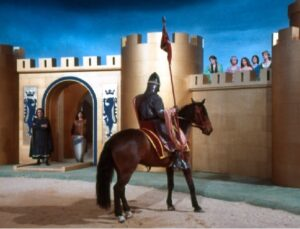
\includegraphics[scale=.5]{a20190313NotesofaLatterDayKnight-img001.jpg}
 \end{wrapfigure}

A knight is made, not born. He may have spent years like the prodigal son, living with the pigs, succumbing to Satan's three temptations of lust, the pride of life, and avarice. In our time, the knight of physical combat may not be necessary, but the knight of spiritual combat is needed more than ever.

\paragraph{Lady Love}
If he is fortunate, he may meet his Love, even if it is unrequited or even unknown. Such Love cannot be consummated carnally, the mistake made by Lancelot and Guinevere.

Her role is to send him on his quest. She chides him harshly when he falls short of the knightly ideal, through vulgarity, personal vanity, or pointless showmanship of his skills. Yet her gentleness inspires him to excel and to become a better man than he ever thought possible.

If you are fortunate, you will be able to see yourself through her eyes.

\paragraph{Duels}
\begin{quotex}
Whatever is acquired by single combat [duel] is acquired with Right. For when human judgment fails, either because it is wrapped in the darkness of ignorance or because it has not the aid of a judge, then, lest judgment should remain forsaken, recourse must be had to Him who so loved her that, by the shedding of His own blood, He met her full demands in death. Hence the Psalm: ``The righteous Lord loveth righteousness." This end is accomplished when, with the free consent of the participants, in love and not in hatred of justice, the judgment of God is sought through a mutual trial of bodily and spiritual strength. Because it was first used in single combat of man to man, this trial of strength we call the duel. \flright{\textsc{Dante, }\emph{De Monarchia}}

\end{quotex}
Combat can lead to the Truth, provided it is not motivated by rage, vengeance, or personal glory.

\paragraph{Initiation}
The \emph{Ordre de la Rose-Croix catholique et esthétique du Temple et du Graal}\footnote{\url{https://en.wikipedia.org/wiki/Salon_de_la_Rose_\%2B_Croix}}, founded by \textbf{Josephin Peladan}, consisted of three grades:

\begin{itemize}
\item \textbf{Neophyte} whose patron was \textbf{Leonardo da Vinci} 
\item \textbf{Chevalier} whose patron was \textbf{Dante} 
\item \textbf{Commander} whose patrons were \textbf{Saint John} and the Holy Spirit 
\end{itemize}
Dante the artist shows the Knight the stages of the journey to Sophia through the Divine Feminine, represented by Beatrice.

\paragraph{Judgment}
\begin{quotex}
Nobility, the quality which I call true aristocracy, requires of a man the recognition of his guilt. In its depths, conscience, which is frequently covered up and suppressed, is always a consciousness of guilt. The necessary thing is to take upon oneself as much guilt as possible and to put as little as possible of it upon other people. The aristocrat is not one who is proudly conscious of himself as first, as a privileged being, and who safeguards his position as such. The aristocrat is the man who is aware of the guilt and sinfulness of this first place, this privileged position of his. \emph{The sense that one is being continually affronted is on the other hand, precisely a plebeian feeling}. \flright{\textsc{Nicolai Berdyaev}} 

\end{quotex}
The knight knows his state of being and judges himself more harshly than any outsider could.

\paragraph{Motivation}
\begin{quotex}
From this deeper principle you must do your works, without a why. I affirm it decisively: even if you do your works for the kingdom of heaven, for God, or your sanctity, although motivated by the other, even then you will not really be in the right. If you ask a true man, a man who acts from his depth: ``Why do you do all your works?" he will answer you rightly only if he says: ``I act only for the action itself." \flright{\textsc{Meister Eckhart}}

\end{quotex}
The Knight follows his Dharma, or Destiny.

\paragraph{Anti-Realism}
\begin{quotex}
The truth or falsity of idealism—and that means if man can or can't give certainty and sense to his life and his experience—cannot be demonstrated theoretically: it can be decided not through an intellectual act, but through a concrete realization. \flright{\textsc{Julius Evola}, \emph{Essays on Magical Idealism}}

\end{quotex}
The animal mind cannot conceive of any reality beyond what appears to the senses. Yet, in the ascent to the divine, sensory images are left behind as one contemplates God and the Angels. Then the Knight returns to his Native Land, seeing through intuition, not the senses.

\paragraph{Intellectual Joy}
The animal mind believes that joy can arise only from sensory objects. Yet the greatest joy comes from intellectual pursuits. When I was a boy around 10 and 11, my parents sent me to weekly classes at the Boston Museum of Science. Afterwards, I would wait in the library to be picked up. My favourite topics were astronomy and mathematics. I learned the mystical symbols for the planets and constellations. I was fascinated with the ancient names of the stars like Aldebaran, Rigel, Betelgeuse, Sirius, Arcturus, so I kept a notebook full of such names.

The library had the four volumes of the \emph{World of Mathematics}. There I read the proof the $1+1=2$ from the \emph{Principia Mathematica} of Whitehead and Russell. I was astounded that those strange symbols could lead to such a result.

Then I learned the names of the Medieval Categorical Syllogisms, such as Barbara, Festino, or Baroco. I am certainly not alone is experiencing such joy.

\paragraph{Ascent through the Hierarchy}
\begin{quotex}
A process of mind is thinking only so far as it realizes the end of thinking, which is always to understand, that is, to see things within a system which renders them necessary. \flright{\textsc{Brand Blanshard}, \emph{The Nature of Thought}}

The evolution of knowledge is, as Plato long ago portrayed it, the emancipation of individual minds from their accidental limitations, and their education into the knowledge of the one real and intelligible world. \flright{\textsc{Bernard Bosanquet}, \emph{Logic}}

\end{quotex}
An animal can only understand individual things. The spiritual knight, however, understands things and events in larger and larger wholes. Individual things are but the reflection of ideas in the Divine Mind. Then the individuals are understood as part of a larger whole. Next, he sees how things develop over time. And so on, until he reaches the more subtle realms. Each such realm corresponds to a level of the angelic hierarchy.

\paragraph{Purification}
The purification of the mind and the will begins in this life. If it is not completed at death, it will be continued in Purgatory. One is not ``sent" to Purgatory; rather, it is the symbolic representation of his state of being at the time of death.

\paragraph{Heaven and Hell}
In the same way, Heaven and Hell are the names for our states of being; that is why there are gradations or levels in each of them.

The vulgar mind images Heaven as an extension of sensory existence, with the exceptions that your truck doesn't break down, your dog doesn't die, and your wife doesn't cheat on you. But none of that can compare to the ecstasy of the Beatific Vision.

The whole divine order is revealed. Then, it is not the individual dog that matters, but rather the essence of the dog is understood in its place in the whole.

Those who choose to live in Hell on earth will simply continue in that state of being. Someone uninterested in holy things now, will not suddenly change course. Hell is to exist without love, so the denizens of Hell hate each other.

\paragraph{The Sannyasi}
\begin{quotex}
To accept suffering in itself and for itself, to consent to it, to seek it, to love it, to make its identifying mark and the very object of disinterested and generous love, to put perfect action in sorrowful passion, to be active up to the point of death, to make of every act a death and of death itself the act par excellence, here is the triumph of the will that disconcerts again nature and that in fact engenders in man a new — and more than human — life. \flright{\textsc{Maurice Blondel}, \emph{Action}}

\end{quotex}
When the knight becomes unable to engage in physical combat, he can become a sannyasi. He will give up attachment to worldly things and eschew the glamour of the world.

The advertisements for retirement communities show happy people riding bicycles with their friends to go play pickle ball. That is how a boy lives, not a man. We are given more years than are necessary to propagate the species. The purpose of those years is to allow time for spiritual development.

\paragraph{Mark of Cain}
The damned are envious of those whom God favours. God favoured Abel, so Cain murdered him. Cain's descendants are numerous; their goal is to overturn the cosmic order. The mark on the forehead from Ash Wednesday is a sign of humility and obedience to the King. Yet the same ashes on Cain's minions are his sign.

\paragraph{Our Spiritual Heritage}
\begin{quotex}
In the last days, God says, I will pour out my Spirit on all people. Your sons and daughters will prophesy, your young men will see visions, your old men will dream dreams. Even on my servants, both men and women, I will pour out my Spirit in those days, and they will prophesy. I will show wonders in the heavens above and signs on the earth below, blood and fire and billows of smoke. The sun will be turned to darkness and the moon to blood before the coming of the great and glorious day of the Lord. And everyone who calls on the name of the Lord will be saved. \flright{\textsc{Acts 2:17-21}}

\end{quotex}
The Sons and Daughters of Europe, the spiritual Knights of the Holy Roman Empire, have been bequeathed the greatest of spiritual and intellectual gifts: Platonic philosophy and the Catholic religion. One to feed the mind, the other, the heart.

Let us not be like the prodigal son who squanders those gifts.



\flrightit{Posted on 2019-03-13 by Cologero }

\begin{center}* * *\end{center}

\begin{footnotesize}\begin{sffamily}



\texttt{Patricia Kay on 2019-03-14 at 14:10 said: }

Thank you, as ever, for your stunning clarity of mind and kindness in articulating Truth in ways that are helpful.


\end{sffamily}\end{footnotesize}

\section{The Law of Success}

\begin{quotex}
Those who make plans will be born to carry them out. Those who make no plans need not be born. \flright{\textsc{Nisargadatta}, \emph{I Am That}}

You are the ``master of your fate" and the ``captain of your soul," by reason of the fact that you control your own thoughts, and, with the aid of your thoughts, you may create whatever you desire. \flright{\textsc{Napoleon Hill}, \emph{The Law of Success}}

\end{quotex}
The question of why some men are successful and others are not has always intrigued me. I am speaking, of course, only of those men who seem capable of great success: they may possess intelligence, creativity, charm, education, good breeding, yet never reach certain heights. In many cases Fortune plays a role, since chance can never be eliminated from life as a factor. Although we typically write from the perspective of the first caste, this post will focus on the second and third castes, that is, those involved in political and economic activity.

\textbf{Napoleon Hill}, in \emph{The Law of Success}, published his study of the characteristics of several successful men of his era\footnote{I am not particularly recommending Napoleon Hill, but am using him as a resource to understand the Kshatriya and Vaishya castes in the contemporary worlds.}. Success, according to him, begins in the imagination, with an idea. Obviously, this is the active imagination, not the passive imagination of daydreaming. Before dismissing this work as just pop psychology, this is just one of the Hermetic and/or spiritual teachings that he adapts to worldly success. A lot of contemporary New Thought or Law of Attraction teachings are distorted or incomplete renditions of Hermetic ideas.

The epigram above could have been written by Julius Evola, for example, who stressed the same inner state of self-mastery. It is no coincidence that Evola was concerned primarily with the Kshatriyas, not unlike HIll. Hill lists several negative emotions or habits—including suspiciousness, jealousy, uncontrolled sexual desire—that are obstacles to success. Enthusiasm, or thumos in our view, must be balanced with self-control. He mentions the Law of Mental Telepathy by which other can ``tune in" to your thoughts. Your self-confidence will be sensed unconsciously by others. These examples can suffice for now.

An important quality for success is the ability to secure cooperation from others. This is called leadership. The main motives that impel men to action are:

\begin{enumerate}
\item The motive of self-preservation 
\item The motive of sexual contact 
\item The motive of financial and social power. 
\end{enumerate}
Those who understand those motives will have greater ability in motivating others. Note that the motive of rationality or intellect and the motive of spiritual development are not at the top of the list. The Leader will try to gain cooperation through group harmony, and endeavoring to convince them so subsume their own interests to the group identity. Hill writes:

\begin{quotex}
Find a motive around which men may be induced to rally in a highly emotionalized, enthusiastic spirit of perfect harmony and you have found the starting point for the creation of a Master Mind. It is a well known fact that men will work harder for the attainment of an ideal than they will for mere money. In searching for a ``motive" as the basis for developing co-operative group effort it will be profitable to bear this fact in mind. 

\end{quotex}
Some leaders know this by chance, while others understand the laws of motivation consciously. What Hill says can be verified: watch the news, read web sites, and try to see them in action. See how group identity and cohesion is formed, for example.

\paragraph{Attraction and Repulsion}
Hill asserts that snap judgments and hunches come from a telepathic connection. Since men are not interiorly united, their audiences will pick up conflicting signals. That is why one man can be associated with widely divergent emotional reactions. Of course, the receivers of the telepathic communication have their own inner limitations, constrained by their three chief motives, which will distort the message. Unfortunately, most people never get beyond this reactive stage, particularly in the political realm. Facebook's success is based fundamentally on clicking ``like", proving the point.

Yet this is to live at the very lowest state of stimulus/response of the etheric body, the pranamayakosha. This is the intellectual life of an amoeba. At least for the amoeba, attraction and repulsion can be a life or death decision, but for humans it just gets in the way of intelligent discourse.

\paragraph{White Collar Criminals and Success}
I will add my own law of industriousness. Few men will actually act on their idea. A major motivator for this blog was my encounter with two white-collar criminals, primarily through their ex-wives. I got to know a lot about them, in great part because the wives held a great admiration for the men, despite the lies, betrayals, and financial decline that came to them.

These men were actually quite industrious in developing their schemes, maybe because it can be more difficult to live a lie than the truth. I got to see a large part of it. Denying their own moral culpability for their crimes, they were quite libertarian in their views. By that I mean that, in their own minds, they never coerced anyone, and their marks voluntarily played their roles in the scam, either out of greed, ignorance, or stupidity. The criminals felt no responsibility for the voluntary actions of their victims.

So I resolved to be industrious, since I have plenty of imagination and self-confidence. I have the first law of a ``definite chief aim", although I doubt anyone has figured it out. Most people who write me privately seem to think all these posts are random and independent, mostly for entertainment purposes. That is because they cannot grasp anything new, but can only interpret new things in terms of what they already know.

I must be low in a ``pleasing personality" and the ability to ``elicit cooperation". The most inane facebook posts get several dozen, if not hundreds, of ``likes". Gornahoor, after weeks of research, and hours of writing from the heart for each post, might get half a dozen ``pity likes". I do appreciate them. We never get invited to speak at conferences or Internet podcasts.

So we are down to our last 50 posts. We could reveal the chief aim in \#1001, or we may just fade away.

\paragraph{The Elusivity of Excellence}
\begin{quotex}
Imagine yourself suddenly discovering that most of your philosophy of life had been built of bias and prejudice, making it necessary for you to acknowledge that, far from being a finished scholar, \emph{you were barely qualified to become an intelligent student}! \flright{\textsc{Napoleon Hill}}

\end{quotex}
The number of men who are able to live by pure reason, the higher intellect, or logos, is very small. The majority are dominated either by eros (sex, desire) or by thumos (anger, ambition). Hence, there will always be an irrational component in political and social life. In Napoleon Hill's conception, reason is to be used for self-preservation, sex, and money. In his own self-development, he came to realize three things regarding worldviews:

\begin{itemize}
\item That you may learn how and where you acquired your philosophy of life, in general; 
\item That you may trace your prejudices and your biases to their original source; 
\item That you may discover, as I discovered, how largely you are the result of the training you received before you reached the age of fifteen years 
\end{itemize}
Even Hill's outlined plan for a more peaceful world cannot overcome that irrational component because it requires the manipulation of emotion.

By a life of pure intellect, I mean one that is dedicated, but not limited, to meditation of Truth, Goodness, and Beauty. This is rare to achieve, but well-worth the effort. Contrariwise, even intelligent and nominally educated people are focused on particulars.

\begin{itemize}
\item They are intrigued by true facts, but not by Truth 
\item They desire good things, but not the Good 
\item They are attracted to beautiful things, but not to Beauty 
\end{itemize}
These all have their deformations.

\begin{itemize}
\item They are intrigued by falsities that confirm their prejudices and worldviews 
\item They desire the pleasurable, even if it is not ultimately good 
\item They are attracted to unusual and abnormal 
\end{itemize}
I was educated in a Boston area school system that tried to teach excellence. The most intelligent, the best informed, and the cultured would be rewarded. However, the leaders of organizations attained, and retain, their positions, not through intellect alone, but because of their skills at organizing, not to say manipulating, others.

\paragraph{Patrician Rulers}
\begin{quotex}
Foolish consistency is the hobgoblin of little minds. \flright{\textsc{Ralph Waldo Emerson}}

\end{quotex}
Since rule by the philosopher-king is unlikely, the best kind of regime is the rule of the gentlemen, that is, of the patricians whose wealth comes from land, not from commercial activity. Because such men are guided interiorly by thumos, there will always be an irrational element in political life. This should be obvious, not just in theory, but also is easily verified empirically. Those who aspire to a life of action should pay close attention.

Whereas the masses are passive and contribute to society by procreation, the gentleman class redirects eros into more creative channels. The desire for fame feeds their ambition to lead and to rule. Such men are necessary despite the risk of bad rulers, who are not fully rational. Napoleon Hill makes the following point, based on his studies of successful men:

\begin{quotex}
All of the great leaders, in whatever walks of life they have arisen, have been and are people of highly sexed natures. 

\end{quotex}
In colloquial terms, these are the ``alpha males". They have an excess of sexual energy that gets sublimated to fame, fortune, and ambition. This separates the successful in worldly terms from the merely intelligent.

A successful system of rule was the Roman consul in the early years of the Republic. There were two consuls, each with veto power over the other. They were taken from the Patrician class and limited to a term of just one year. The idea of being a professional politician, such as we see today in the so-called Western democracies, was anathema. Today's professional politicians become skilled at just one thing: the learn how to manipulate the political system. The Patrician, on the contrary, had demonstrated his skill at being successful in the world, as was committed to the welfare of the nation, not to a political faction or party.

To jump ahead a couple of millennia, we can look at the phenomenon of \textbf{Donald Trump}. Let's detach from the spontaneous arising of either attraction or repulsion, often associated with him, and consider him as an archetype. Since the plantation system ended some time ago, Trump is the closest we have to a Patrician, having achieved financial success primarily through real estate rather than buying and selling, or worse. Moreover, he is an ``outsider" to the political system. Like him or not, you would have probably felt the same way about particular Consuls. If his personality of off-putting to you, consider that a man cannot achieve such worldly success by being just like you. A young mother of four sons despises him, so I posed a question to her. Suppose a gypsy fortune teller offered these predictions for your sons:

\begin{enumerate}
\item One would get an MBA degree from Wharton, one of the top 3 business schools in the country. 
\item The second son would make a billion dollars developing real estate around the world. 
\item The third would become a big TV star.\footnote{I have never watched an episode of the Apprentice.}
\item The fourth would run for president and defeat 16 other professional politicians 
\end{enumerate}
Objectively that is quite a resume and what mother would be displeased with that prognosis? Now I would prefer a Patrician to have more of that Roman dignity than we see in Trump. Nevertheless, in a democracy we can only vote for what is available. The question is still open: what kind of a man (or woman) do we admire? Someone who became wealthy by capitalizing on political connections? And excelling at party politics is hardly a skill worth bragging about.

Learn from this, all who aspire for leadership. It is never a matter of just winning intellectual arguments on abstruse issues. And minor contradictions don't matter. The intelligentsia – that is, those who earn a living solely on words like journalists, lawyers, and so on – get exercised by so called ``gotcha" questions: a minor inconsistency, an offensive remark, etc. In that way, they become totally oblivious to the actual world, mistaken their purely verbal formulations for reality itself.

\flrightit{Posted on 2016-05-26 by Cologero }

\begin{center}* * *\end{center}

\begin{footnotesize}\begin{sffamily}



\texttt{Thomas Blanchard on 2016-05-26 at 11:20 said: }

I'm curious on what you base your assertion that Napoleon Hill is primarily concerning himself with Kshyatrias. His goals and attitude seem quite bourgeois – after all, you note that he puts reason at the service of self-preservation, sex, and money. You note that you're referring to both the Kshyatria and Vaishya castes, but what differentiates them? Is it the role of thumos dominating the soul versus eros/material appetite?


\hfill

\texttt{Cologero on 2016-05-26 at 12:20 said: }

I need a little poetic license here, Thomas, and I thought it was clear I was not recommending Napoleon Hill as an authority. At the end I wrote: ``to understand the Kshatriya and Vaishya castes in the contemporary worlds". So the intention was to describe the contemporary manifestation of the castes, not their traditional roles. To give him his due, however, is it bourgeois to achieve self-mastery over your own thoughts? In describing the situation of the modern world, I took as a source someone who has studied successful people in that world. The laws of power have not changed over the centuries, however.

Hill is not putting reason at the service of …, he is describing what people actually do. The source for the thumos comment is actually Plato: to the extent that rulers are led by thumos, there will be a residue of irrationality in politics.

The roles of the two castes are hard to differentiate today. Consider how much debate there is about the influence of commercial interests over the political process.


\hfill

\texttt{Pickman on 2016-05-26 at 13:50 said: }

What good will it be to reveal the chief aim in the last post when it can no longer be debated? Why not now?

The reason this blog gets so little attention is simply because of its lack of marketing. It has great content but it's aesthetic presentation and outreach are rather muted. Whereas slick `all style/spin and no substance' propaganda gets the masses attention. It has always been the case (perhaps an inversion of recognisable quality) but that is just the way the world media works.


\hfill

\texttt{Jacob on 2016-05-26 at 19:38 said: }

Cologero, I'll be very sad when the posts on this blog end. I have always felt that you were the most insightful author I have ever read. I say this not as flattery, but because I believe it to be true. I often feel so alienated from the world today with its constant focus on desire and nothing more. At the same time I realize that I do need to be more industrious with the knowledge I have. Recently, I have begun to treat your writings in a way many treat sermons. Get a message that confirms my worldview and continue on without any deep reflection. In any case, thank you for your time. 

On Trump: I am deeply conflicted because I really like how he is willing to bravely deny the tenets of the Left. However, he seems to be sign of our age as well. The man who is the most entertaining and outlandish gets the most attention. It's possible that he is using the tenets of post-modernism to achieve higher goals (riding the tiger), but I don't see any evidence that he has any knowledge of anything higher than power. Still it's better to take a bad leader who establishes order than complete chaos right? I'm almost to the point that withdrawal from the world (especially in politics) sounds like an appealing option.


\hfill

\texttt{Matt on 2016-11-09 at 05:15 said: }

All those pundits trying to predict the presidential election would have done themselves a service by reading this post.


\hfill


\end{sffamily}\end{footnotesize}

\section{The Holy Knights Templar}

It is unnecessary to summarize here the entire history of the \textbf{Knights Templar}, which can be found easily enough online, so we will just highlight certain points that are of interest. Ultimately, our goal is to consider the option of a Fourth Order of the Templars.

The Templars conjoined the two greatest archetypes of Tradition: the ascetic and the warrior. As is well-known, the great Church Doctor \textbf{St. Bernard of Clairvaux} created the \emph{Rule for the Knights}, adapted for them from the \emph{Rule of St. Benedict}. That is available as \textit{In Praise of the New Knighthood}\footnote{\url{http://digihum.mcgill.ca/~matthew.milner/teaching/resources/docs/clairvaux_newknighthood.pdf}}.

Such an order of knights is hardly possible today, first of all because there is no desire among the hierarchy for such a venture. The other obstacle is that the means of warfare have changed so much. The various means for mass destruction have eliminated the role of the Knight. Although the ideal of the warrior ethic still exists, it has been incorporated into the special forces in the military services of secular states.

Nevertheless, the romance of the Knights Templar persists, despite or, in some cases because of, their ignominious end. The Traditionalist order of the Society of Saint Pius X\footnote{\url{https://sspx.org/en}} sells an audiolecture \textit{The Knights Templar}\footnote{\url{https://angeluspress.org/collections/church-teaching/products/knights-templar}} as well as a written history, \textit{The Templars: Knights of Christ}\footnote{\url{https://angeluspress.org/products/templars-knights-christ}}.

Hence, the last Templar grandmaster, \textbf{Jacques de Molay} ought to be a candidate for sainthood as a martyr for the faith. Instead, due to his fabricated condemnation by both Throne and Altar, Freemasonry — the enemy of the Church — has claimed him as one of their founders.

\paragraph{Ludibrium}
There are two ways to do history. The ordinary way is two-dimensional, that is, the goal is to describe the relationship of physical events over the course of time. The esoteric way is three-dimensional history which is more concerned with identifying the spiritual forces that underlie material events. Among those factors are ``archetypes" which are mythological motifs that manifest themselves repeatedly, in different forms, throughout history. The motif that we are interested in is that of esoteric and exoteric teachings. The esoteric teaching will assert itself, often in apparent opposition to the exoteric teachings. However, our goal is always to unite them.

Following the breakup of the Templars, some of them were absorbed into the \textbf{Order of Christ} in Portugal, and others returned to the East where they were first formed. The story is that the Templars reformed as the Rosicrucians who emerged publicly a couple of centuries later. \textbf{Johannes Valentinus Andreae} published the \emph{Chymical Wedding of Christian Rosenkreutz}, one of the manifestos of the Rosicrucians. He referred to that document as a \emph{ludibrium}, that is, play. This brings to mind Valentin Tomberg's ideal of turning work into play. Secular historians will only be satisfied with material connections between events, but the third dimension will look for the reappearance of related ideas. The obvious clue is that a ``secret" society will not be publishing manifestos.

\paragraph{The Knights Kadosh}
\textbf{Albert Pike} in the chapter Knight Kadosh\footnote{\url{http://www.sacred-texts.com/mas/md/md31.htm}} from \emph{Morals and Dogma} adds to the mythical history of the Templars. He asserts that the first Knights took their vows before the Patriarch of Constantinople. That is incorrect; it was the Patriarch of Jerusalem. He then claims that the Templars had both an esoteric teaching, the Church of John, and and an exoteric teaching, the Church of Rome. He implies that the exoteric teaching a smokescreen to hide the true teaching. However, there cannot be any conflict between the esoteric and exoteric teachings. After all, the Templars were quite devout in their exoteric practice.

Nevertheless, the destruction of the Templars did have consequences. Pike claims that a remnant of the Templars continued under the auspices of Freemasonry. Their goal was to ``to overturn the Throne and the Altar upon the Tomb of Jacques de Molay". Having ended the French monarchy, they directed their efforts against the Pope. At the time that Albert Pike was writing, the second part of the task was incomplete. However, were he alive today, he may be less sanguine about the ultimate success of the revolution.

\paragraph{A Dilemma Resolved}
Pike implies that the revolution was a Pyrrhic victory, since the successor of the Templars perished, i.e., there is no longer a direct — or real — relationship to them. Therefore, we turn instead to the ideal relation\footnote{\url{http://www.gornahoor.net/?p=8282\#relations}} and ask the same question. Pike makes the distinction between the Johannine and the Petrine current in the Templars. By rejecting the Petrine, he implies that the Rosicrucians and Freemasons are the heirs of the Johannine current. However, there has been revealed a more complete way to regard those currents.

The Russian esoterist \textbf{Valentin Tomberg} met with some students who had studied under Professor \textbf{Gregory Mebes}. In that group there were three grades: Martinist, Templar, and Rosicrucian. Certainly, then, Tomberg was immersed in the Johannine current. Nevertheless, he came to the realization that any doctrine of ``two churches" was false. The Church of John was not a rival to the Church of Peter. Rather, their relationship was described this way:

\begin{quotex}
The mission of John is to keep the life and soul of the Church \emph{alive} until the Second Coming of the Lord. This is why John has never claimed and never will claim the office of directing the body of the Church. He \emph{vivifies} this body, but he does not direct its actions. 

\end{quotex}
Hence, the spiritual current of the Templars belongs with Rome, although only the SSPX seems willing to revivify that connection.

\paragraph{A Fourth Order}
A latter-day Templar revival would not be a first, second, or third order, since it is a lay initiative, but a fourth order. The masonic temptation is to build, and this needs to be avoided. Hence, that would rule out much of what is called an ``intentional community". The alternative is a community that grows organically. Instead of a top-down model, that more traditional idea of subsidiarity\footnote{\url{https://gornahoor.net/?p=2554}} is appropriate. Hence families would develop into phratries, and then tribes, in a natural way.

The Knights Templar was restricted to those already knighted. Moreover, each knight turned over his assets to the community. That would not be appropriate for a lay group. A family corporation\footnote{\url{https://info.legalzoom.com/establish-family-corporation-21136.html}} of some type would be fairer, and it would make it easier to leave without causing legal problems.

\paragraph{Entryism}
An Order needs to have a spiritual centre. One viable alternative is to affiliate to an SSPX chapel. Not only would there be a friendly atmosphere for medieval values, but a relatively small group would be able to exert influence. I will offer some specific suggestions in the mailing list.

The Templars survived for two centuries, and their demise was not the result of any internal tension. That is because they inserted themselves into a larger organisation, which granted legitimacy, cohesion, and spiritual support. Self-existing alternative movements today typically claim a factitious membership based either on a non-existent genetic similarity, or else the adherence to some small set of propositions. The first alternative cannot settle legitimate and important differences of opinion, and the second alternative is no different from the modern world.

Building an organisation from scratch outside of existing institutions is a daunting task. Even in democratic situations, the formation of new political parties – while theoretically feasible – has been totally ineffective in practice.

\paragraph{Distinctiveness}
There need to be outward distinctions, while not appearing to be overly eccentric. Obviously, a certain modesty in dress and the avoidance of much of popular culture would be mandatory. In another post, we will adapt the Rule proposed by St. Bernard of Clairvaux to make specific recommendations for lay groups. Of course, there will need to be some latitude for local groups to determine some of their own customs.



\flrightit{Posted on 2017-07-05 by Cologero }

\begin{center}* * *\end{center}

\begin{footnotesize}\begin{sffamily}



\texttt{James on 2017-07-05 at 02:26 said: }

Thanks for the great post.Looking forward to the next post on the subject.


\hfill

\texttt{Aleksandar on 2017-07-05 at 03:42 said: }

"The Templars conjoined the two greatest archetypes of Tradition: the ascetic and the warrior."

I've been fascinated by this topic for quite some time. This is much needed today. A purpose for a man of traditional values, physically and mentally trained and disciplined individual, perhaps skilled in martial arts, or at least in tune with the heroic pathos, who at the same time avoids, much as possible, modern day degenerate influences designed to numb down, absorb and dissolve. What is left for him in today's world? One who assimilates two paths which are today artificially divided. Unfortunately, at the gym I mostly witness brutes and meatheads. Same thing with others who indulge in a more physical aspect of life. Who says that you cannot do all of that and same time cultivate your mind – not in a pseudo intellectual way, of course, working on your "brain sharpness" with self help books and pseudo yoga manuals, but through active involvement in the entertainment of higher ideas based on the true traditional knowledge?

Knight is now reduced to a mere expendable, mercenary, a cog in the wheel without a Divine guidance and higher purpose except serving the secular order. Modern day ascetics (not counting monks) are in some way NEETS, hiding away in the shadows but devoid of that Divine impulse to overcome their nihilistic state.

This is why I'm also interested in the phenomena of another archetype which reemerged in last few years (or decades) – a paladin. Similar to a Templar, a popular RPG class played by thousands, if not millions of kids (and adults) across the world in different fantasy video games. Paladin is based on Charlemagne's Twelve Peers, offering an image of ideal, heroic knight whose strength comes through religious devotion and asceticism. Sadly, many of these life options are now limited to a mere fantasy game, a role play. An impulse is certainly there, as evidenced in a certain rise of popularity of medieval knights, military orders and history through the online communities (ignited by the current events in the West, no doubt).


\hfill

\texttt{Fred on 2017-07-05 at 06:59 said: }

Very good article, I will mention two things that can inspire a reflection.

In the Parsifal of Wolfram von Eschenbach, without a doubt an initiatic poem, the guardians of the Graal are called Templars and have white capes. Eschenbach himself was a knight.

About the remarks of Albert Pike I really want to point to the fact that the direction of the subversive project of modernity is usually closely tied to degenerated initiatic groups. In fact every error of modernity is a perversion of a traditional principle. For example liberty, equality and fraternity. It is explicitly evident in the pantheism of Spinoza and Giordano Bruno, clearly arised from their own misinterpretations of hermetic and kabbalistic texts. So, freemasonry was the pretorian guard of tha anti-traditonal englithenment, as natural for a subverted esotericism. The same can be said for jews.


\hfill

\texttt{willehalminstitute on 2017-07-05 at 12:18 said: }

@Fred: The ``Templeisen" as they are called in Middel High German in Wolfram's Parzival cannot be the same as the Templars, at most their forerunners, because the Grail events described in Parzival took place in the 9th century, while the Templars only surfaced some two centuries later. I am basing myself on the research by Werner Greub in his book ``How the Grail Sites Were Found – Wolfram von Eschenbach as a Historian" (see Grail Sites at \url{http://www.willehalm.nl}) that I translated and published.


\hfill

\texttt{THAT on 2017-07-05 at 18:27 said: }

It is a commendable initiative, but the fact that we know so little about the true nature of the secret doctrines and initiations of the original Templars makes the appropriation of the Templar identity by modern groups problematic. It will be based merely on the exoteric Templar image; anything more than that would be speculative. 

And if entering into speculation, it is not outside the realm of possibility that the Templars did in fact have secret doctrines and practices, at least for the elite of the order, that were heretical and not merely a harmonious deepening of Catholic Christianity. Evola seemed to believe that much in his `Mystery of the Grail'. The fact that they were exoterically devout Catholics proves only that they didn't really have any other choice than to pay lip-service to it.

De Molay and the Templars took high interest on loans in their role as bankers, and this at least doesn't add credit to the sainthood account. 

What speaks strongly in favour of the Templars is of course Dante's support for them. Charles Upton, in the chapter ``The Templars, the Freemasons and the Counter-Initiation" in `Vectors of the Counter-Initiation'. suggests that there may have been within the Templar complex both a stream of corrupted esoterism and a valid Christian current. The Templar-connected stream inverting the resources of their initiatory current for the sake of worldly power would have gone underground and seeded various conspiracies. Much of this is speculation that cannot be proved, but the most vital resources and secrets of the Templars were saved from the persecutors, and I find it hard to believe that the underground stream seeded from this wealth of initiatory empowerment was ever discontinued. I tend to believe this lineage may still preserved by certain privileged and secretive elitist circles, but perhaps in a corrupted form.


\hfill

\texttt{Fred on 2017-07-05 at 19:46 said: }

While the role of freemasonry as a counter-initiatic source demand that we at least acknowledge the possibility of counter-initiation and errors among the Templars there are several factors that witness in favour of the Knights.

First of all Dante and St.Bernard, then the fact that they were killed by King Philip IV, the man who did more than anyone else to undermine the two universal authorities of the middle age: the Pope he submitted and brought to Avignon, and the Emperor (France was the first of the great kingdom of Europe to declare the authority of his King as the highest and rejecting any nominal submission to the Emperor).

While a French puppet the Pope even intended to pardon the Templars, as shown in the Chinon parchment.

They were killed by the King who was the living embodiment of the ksatriya revolt against the traditional order of the medieval Christendom/Europe.


\hfill

\texttt{THAT on 2017-07-06 at 09:59 said: }

St. Bernard marks the beginning of Templar history. I do not think there is any reason to assume they would have been corrupt from the beginning; so the Templar ideal as partly forged by St. Bernard would be valid no matter what eventually developed at the expense of its original purity within the shadows of the Order. 

One subject for much speculation has been to what extent they were influenced and changed in their inner orientation and agenda by finds (some of which may have accelerated their rise to massive power; did this power go to their heads?) that they made in the East and by their contacts with various gnostic groups. The Order of Assassins, for example, was counter-initiatic in the extreme.

I am aware that the Templars were pardoned, but this could just as well be interpreted as a political move not necessarily based on objective truth, aimed at keeping the exoteric romantic legacy of Templarism as part of Catholic mythology; once the Templar organisation no longer represented a practical problem, one could conveniently forget about the shadowy esoteric affairs and honour the aspects of Templar history deemed good. I am not saying this has to be the right explanation, but it is a reasonable possibility. 

What you say make for a good case, but the fact that corrupt forces are involved in a persecution does not guarantee that the persecuted is not corrupt as well. In all probability the case of the Templars is far more complicated than is allowed for by the one-sidedness often seen both in their accusers and apologists.


\hfill

\texttt{Cologero on 2017-07-07 at 22:58 said: }

Interesting comments. I'll try to integrate them into another post, but here are some loose ideas in the meantime.

When I was a boy, one of my favorite TV shows was about a Paladin: Have Gun, Will Travel\footnote{\url{https://www.youtube.com/watch?v=HAoEOhsGJyU}}. The archetype is surely alive doay, although hardly manifestable in the modern world, maybe like Junger's ideal of the Anarch. Unfortunately, it seems that in today's pop culture, that ideal has deteriorated to a wise-cracking wise guy, nearly indistinguishable from a sociopath.

The widespread image of Jacques de Molay depicts him with long hair and wearing a long flowing robe. St. Bernard specifically rejected that image of the Knight, and insisted the Templars keep their hair short. The lesson: be wary of any historical reconstructions of the Knights.

As for their sanctity, Bernard referred to the Knights as ``holy martyrs". The contemporary witnesses to Molay's execution regarded him as a martyr, and collected relics. So the idea of sainthood is not so far fetched. Usury is more subtle. Perhaps you can categorize the Templars as usurers, if you regard their fees a mere ``loopholes". The argument contra usury, it seems, is based on the misconception that money is constant. If I borrow a cup of sugar, I can return a cup of sugar in 6 months. I can bake a pie now and you can bake one using the same recipe in 6 months. But if I borrow \$5 to buy a bag of sugar now, there is no guarantee that you will be able to buy a bag of sugar when I return the \$5 in 6 months.

I think there is a misunderstanding about the esoteric/exoteric distinction. Without using those specific terms, Bernard alludes to the distinction several times in his ``In Praise of the New Knighthood".E.g., he wrote ``we must not let this literal interpretation blind us to the spiritual meaning of the texts [i.e., scriptures]". He mentioned how the commoners would receive the ``milk" of doctrine, while the Knights would understand the ``meat". The latter would include the recognition of the divinity in man and the spiritual sense hidden beneath the written word. The point is that the esoteric and exoteric are intimately related, even if the former is reserved for the few. Fundamentally, the esoteric is not some new ``secret" doctrine, but rather a much deeper understanding of the exoteric doctrine. Anything else is subversion.

Please consider the distinction made between real and ideal relationships. We are not looking for an ongoing material secret transmission [``real"] of the Knights, but rather the reappearance in space-time of transcendent archetypes [``ideal"].


\hfill

\texttt{THAT on 2017-07-08 at 08:15 said: }

I concur with your understanding of the exoteric-esoteric spectrum. Obviously I didn't mean to imply that `esoterism' amongst the Templars must naturally and inevitably l have been some heretical `secret doctrine' and so on, only that it is quite possible that the Order might at some point have come to secretly house such subversive elements, that would have inverted the original esoteric intention to some degree.

The ``meat of doctrine" to which you refer was most clearly expressed in the case of Meister Eckhart, and that didn't go so well for him; this is the greatest weakness of Catholicism, as it leads exactly to the formation of ``secret doctrines" that may become subversive, when the church doesn't allow for a smooth and continuous transition to open esoterism that is accepted as a deepening of exoteric doctrine.

I am not so knowledgeable about the question of usury, but you—and I apologize if I misunderstand you here—seem to be making too lightly of it; both Christianity and Islam have taken a rigorously strict approach to the question from the beginning, and this is because usury is a means that belongs to the Enemy. Any organisation touching upon it makes a compromise with him.

Speaking of the Enemy—and relating to your mentioning of entryism—it would be valuable to consider how this `order-to-be' might guard itself against the infiltration of agents of subversion, of whom there is a never-ending supply these days. 

I understand what you explain about `real' and `ideal' relationships, and that the ideal and archetypal relationship is intended in the case of this project; I only expressed the suspicion that an actual uninterrupted Templar transmission of some kind may still be running underground as part of ``occult" elite operations. The possibility must be kept in the back of the mind as such forces might take special notice of any rising contemporary `movement' connecting with the Templar archetype.


\hfill

\texttt{Fred on 2017-07-08 at 15:40 said: }

I always felt the ``meat of doctrine" much more in line with Catholicism in the allegorical esotericism of Amor than in Eckhart.

Maybe this is because I'm italian but I see Dante, the Roman de la Rose and chivalric novels more closer to St.Bernard. As a cultural expression it feel much closer.

Eckhart was a german spirit, his emphasis on detachment feel almost buddhist to me. His problems with the inquisition were caused by the words he used: alien words to the culture of Latin Christianity.


\hfill

\texttt{Old Chap on 2017-07-09 at 12:32 said: }

The downfall of the Templars shows us that such Orders and their slavish adherence to certain values is foolish in a world and a time where authentic, not superficial morality is a rarity. Since we live in a world without morals and just laws (where they exist on paper they are not followed in reality), all of these old sacred designs are simply impossible on any substantial scale. The fault lies with human nature which is markedly flawed, rather than a nonexistent elite which will never appear (still waiting for Christ's return and all the other prophesied saviors of mankind). Faith alone does not supersede reality no matter how much one wishes otherwise. Chivalry is dead because there is no longer a use for it, as it would be an undeserved relic for a people more concerned with gossip and ``winning" and consumerism and the endless array of meaningless ``activities" and entertainments. (Just my two pence.)


\hfill

\texttt{Harharkh on 2017-07-10 at 14:55 said: }

You live in fantasy land, old man.


\hfill

\texttt{Cologero on 2017-07-10 at 21:35 said: }

Yes, grasshopper, and when you realize the illusory nature of your own existence, then you, too, may become enlightened.


\hfill


\end{sffamily}\end{footnotesize}


\chapter{Return to Tradition. The Future Elite}
\section{Lightning Strikes from the East}

\begin{quotex}
Ignorance pure and simple is far preferable to false ideas. \flright{\textsc{Rene Guenon}}

Lightning cometh out of the east, and appeareth even into the west. \flright{\textsc{Jesus Christ}}

\end{quotex}
In \textit{East and West}, \textbf{Rene Guenon} outlines a plan for the recovery of Tradition in the West. Obviously, the plan is complex and requires some unique skills as well as intellectual depth to succeed, and it is something he doesn't expect to happen next week. Nevertheless, it is well worth elucidating in detail, if only for the boons it will bring to those who make the effort to understand. However, we take it seriously as we heed Guenon's warning\footnote{\url{https://www.gornahoor.net/?p=35}} about the consequences of not undergoing a consciously led social transformation. These are either a fall into complete barbarism or else the assimilation to another Traditional culture, most likely following a period of social upheaval. The plan must take place on three levels:

\begin{enumerate}
\item The knowledge and understanding of metaphysical principles 
\item The recovery of traditional sciences 
\item The transformation of the social order 
\end{enumerate}
\paragraph{Return to Intellectuality}
First of all, it is necessary to understand the goal, or what exactly defines a traditional civilization. Guenon explains:

\begin{quotex}
What we call a traditional civilization is one that is based on principles in the true sense of the word, that is, one where the intellectual realm dominates all the others, and where all things, science and social institutions alike, proceed from it directly or indirectly, being no more than contingent, secondary and subordinate applications of the purely intellectual truths.

\end{quotex}
To be blunt, the intellectual truths he is talking about are not debating points; they are either understood or they are not. The thinking, willing, and feeling functions must be understood in their proper relation. This is especially true in our age with its emphasis on action for its own sake and sentimentality. Guenon writes:

\begin{quotex}
The pure idea has no immediate relation with the domain of action, and it cannot have the direct influence on outward things that sentiment has; but the idea is, none the less, the principle, the necessary starting point of all things, without which they would be robbed of any sound basis. Sentiment, if it is not guided and controlled by the idea, brings forth nothing but error, disorder, and obscurity; there is no question of doing away with sentiment, but of keeping it within its legitimate bounds.

\end{quotex}
The dominance of sentimentality is expected in the modern mind, but it seems to be none the less present even among some segments seeking a return to tradition. So we must insist on this initial understanding, as Guenon explains:

\begin{quotex}
Thus a return to tradition and a return to principles are in reality just one and the same thing; but clearly the knowledge of the principles, where it is lost, must first be restored before there can be even a remote thought of applying them; it is quite out of the question to build up again a traditional civilization in all its fullness without first having the supreme and fundamental knowledge that must preside over the work.

\end{quotex}
\paragraph{Return to Tradition}
Since the time Guenon's book was published, much has changed in the West. On the one hand, the knowledge of Eastern systems such as the various schools and sects of Hinduism as well as Buddhism, has become much more prevalent, even to the point of attracting many adherents. On the other, there are the many alternative, or New Age, types of spiritualities, primarily deriving from Theosophy and similar movements. The latter consist of a strange mix of not fully understood principles heavily infused with mushy sentimentality. The former, although they show some promise, are too often incompatible with the Western mindset and style of life. The adherents either adopt alien styles of dress and mannerisms which are quite secondary to the intellectual principles or else end up accommodating the Eastern teachings to Western prejudices and, in the process, compromising what is authentic in them. That is why Guenon suggests:

\begin{quotex}
In our eyes, the most satisfactory solution for the West is the return to her own tradition, completed where necessary as to the domain of pure intellectuality.

\end{quotex}
Now, this requires some explanation since the Western mind is so imbued with egalitarianism, even among those most loudly calling for a return to Tradition. This domain of intellectuality is only suitable for the small minority, or elect, who are capable of understanding. For the rest, there needs to be an exoteric religion that bears these principles in a more palatable form. Hence, we witness the many discussions, often heated, about a return to Christianity or some sort of neopagan revival. That debate is not of interest to the elect who understand that metaphysics and religion need not be in the least incompatible. Guenon writes:

\begin{quotex}
Even if the West repudiates sentimentalism (and we mean by that the predominance of feeling over intelligence), the western masses will retain none the less a need for satisfactions derived from sentiment, which the religious form alone can give them, just as they will retain a need for outward activity.

\end{quotex}
There are certainly some manifestations of Western thought that are of a high intellectual caliber. Unfortunately, they are ignored by contemporary leaders of the Western religion who falsely believe they are in continuity with that tradition. Or else, they are depreciated and rejected by others because the Western tradition is ``\emph{too high for them}", as Guenon writes. The latter go searching in vain for an elusive ``authentic" tradition, when they can't even understand the one that is closest in time to them. We will bring what Guenon has to say on this topic at a later date.

\flrightit{Posted on 2012-01-17 by Cologero }

\section{Recovering Tradition}

\begin{quotex}
Gradually there will revive in Christendom the forgotten, deeply sleeping, and perished treasure of wisdom and sacrificial deeds of the past — right back to the primeval revelation and the paradisiacal state of mankind. Thus all truth and all love of all times will have their home in the Church of Christ, which will then be the all-embracing (catholic) unity of all things and all beings who are striving for timeless values — in the sense of realizing the ideal of one Shepherd and one flock. The words of the Creed: ``I believe in one holy, catholic and apostolic Church" receive their full significance when the Church becomes universal (catholic) not only in space but also in time, i.e., when it embraces not only all peoples of the present, but also times of the past. \flright{\textsc{Valentin Tomberg}}

\end{quotex}


In recent posts we have been delineating the characteristics of a Traditional society, so that those so inclined would know what to work towards. Moreover, we emphatically deny that there is such a movement or school as ``Traditionalism" or that a man can be a ``Traditionalist", \emph{sensu stricto}. ``Traditionalism" is a term without content, unless its content consists of the valid Traditions. In other words, one cannot be a Traditionalist, that is, a man who follows Tradition in general; rather, one must follow a particular Tradition. Of course, in a Traditional society, that means one follows the Tradition he is born into, the advice given by the French magician Eliphas Levi. Guenon held the same position, except for those rare men who are beyond caste and hence free to follow the Tradition of their choice.

For the Westerner of today, that Tradition should be Catholicism, although it is now barely recognizable as Traditional. A case can be made that one of the European paganisms is the natural Tradition of the West, and this seems plausible to many since paganism has been in the unconscious of the West and is now beginning to reawaken; or, as Stephen Flowers puts it, ``Odin has been sleeping." He is well read in this field and has done much to reconstruct or resurrect the ancient Germanic religion. I shall be speaking of the former, since I am more familiar with it; nevertheless, the basic points will apply to both identically.

First of all, the question recently came up about whether Christianity contains the seeds of its own destruction. We need to point out that every human movement, even divinely inspired, will gradually run down; this even happened to paganism, which yielded to the newer religion. This is a spiritual law. After the initial conscious impulse, a movement then continues mechanically, declines, and eventually may even become the opposite of how it started. Periodically, conscious impulses must be applied to it, to set it back on its course.

Unfortunately, what is called Traditional Catholicism does not go back far enough, since its tradition stems from the counter-reformation at Trent, when it really needs to go back much further. For example, it needs to rehabilitate the likes of \textbf{Dionysius the Areopagite}, \textbf{Clement of Alexandria}, \textbf{Origen}. The idea of \emph{gnosis} needs to be restored. The idea that \emph{theosis} is required for salvation, not faith alone, must be taken seriously once again. The philosophy of Plato and the Neo-Platonists must form the human side of divine revelation (not a replacement for it). These ideas are not novelties, quite the contrary, they are the true Tradition.

Of course, due to the differences in human nature and the law of castes, not everyone will be capable of understanding things in this way. But the elite will do so, even in not a public way. The warriors will need to apply these teachings to particular circumstances, not because they are more manly, but because that is the law for their caste. This is why a Traditional society is not a theocracy: the elite teach the principles; the warriors and producers apply them.



\flrightit{Posted on 2010-03-16 by Cologero }

\begin{center}* * *\end{center}

\begin{footnotesize}\begin{sffamily}



\texttt{Comprehensor on 2010-03-18 at 18:14 said: }

Though many Westerners are born into Catholicism it is a dead religion (i.e. it no longer possesses the spiritual influence) and so what is it they are really born into? Something which is beyond their understanding and reduced to an egotistic historicism, moralism, sentimentalism, and messianic marxism. Even if there were some of the church hierarchy who had any real knowledge of tradition other than their theological hogwash the church has such a bad reputation that to fix it one would have to purge it of nearly all its ordained members. And all of this impossible work would be for naught because quite simply Christianity is far to sentimental and Semitic a form, which is in direct conflict with the Aryan spirit. What the traditional man should be focused on today is in taking the essential aspects of Aquinas, Eckhart, and Boehme, mixing it with the Vedanta and Yoga, and applying it to their own ethnic tradition, that is, reconstructing the old ``pagan" paths. Above all, one needs to receive an initiation into the lesser and greater mysteries to have any qualification at reconstructing a tradition, and this initiation can only come from living traditions, either Sufism, Hinduism, or Buddhism.


\hfill

\texttt{Cologero on 2010-03-18 at 21:31 said: }

Yes, I agree with your project in outline, but the devil is in the details.

I would add that the core of Western esotericism has been Hermeticism … both Guenon and Evola agree on this. Evola, however, insists this is really a pagan movement. Of course, its origin is pagan, if we follow the progression

Hermes Trismetigistus $\rightarrow$ Pythagoras $\rightarrow$ Plato $\rightarrow$ Plotinus

Nevertheless, this trend buried itself in the dominant religion of the West, as we see from the grail legends and various thinkers such as Dionysius, Clement of Alexandria, Origen, Ramon Lull, Ficino, and so on. Two recent attempts, both by Russians, have attempted once again to integrate Hermeticism, viz, Valentin Tomberg and Boris Mouravieff. It remains to be seen if they create a lasting impact.


\hfill

\texttt{Comprehensor on 2010-03-19 at 00:21 said: }

The devil I would say is the industrial-capitalist civilization which is in no way compatible with tradition and culture.


\hfill

\texttt{Cologero on 2010-03-19 at 05:04 said: }

I'm afraid that is just a symptom, the result of the degeneration of castes. Only a regeneration is the cure, not a revolution.


\hfill

\texttt{Comprehensor on 2010-03-19 at 05:50 said: }

Whatever it is it is here. Modern education, technology, machines, spoonfed consumerism–all of this ruins the mind physically and psychically, and it is only on course to become much worse. The masses aren't going to bend a knee to any initiatic elite, nor are they interested in initiatic regeneration. Most people think that initiatic rites are either satanic or imaginary. This being so how much further removed are they from intellectual principles? And as far as the people who have assumed the functions of the rulers, warriors, and priests, they are all rather pathetic–with very few exceptions–and no elite would waste their time trying to teach those who are corrupted to their very core. A restoration of tradition would take the miracle of all miracles.


\hfill

\texttt{Cologero on 2010-03-19 at 09:43 said: }

The masses will believe any old thing and can change in an instant … they are not burdened with gnoseological questions. It would be better that they believe something true rather than false.

The elite do not kvetch. The elite, and I mean the warrior elite, have the will to power, the power to impose their will. After the disintegration of the Western half of the Roman Empire, the Occidental world was in worse shape than today. The elite went back to the sources and modeled themselves after the great pagans: Hector, Alexander, Julius Caesar, Vegetius, Scipio. Where is that elite today? Who today knows anything about Charlemagne, Arthur, Boucicaut, Godfrey de Bouillon? Forget the principles, all the principles anyone needs are on this blog. That is really for the tiny few, who are ineffectual in the world without the Ksatriyas to actualize those principles in the world. Forget the paleo, neo, new, alternative rights … go back to the beginning.


\hfill

\texttt{Comprehensor on 2010-03-19 at 17:38 said: }

Principles are NOT for a tiny few. They are the backbone of the entire civilization. For a return to tradition we require a complete change of everything modern. That is a mammoth task and no will to power can achieve that. I do not consider Alexander and Caesar great pagans, but rather the enemy. They turned away from the sacred to wage destructive wars and to create a universal empire. I am more interested in preserving unique ethnicities and unique cultures rather than making one great ``European Empire." Moreover, I am opposed to the exoteric/esoteric model which limits the esoteric to a tiny few. We need to do away with that entirely and move to a more metaphysical and participative system like Hinudism which doesn't have this distinction.


\hfill

\texttt{Cologero on 2010-03-21 at 02:01 said: }

Despite many efforts, several misconceptions persist.

We agree, principles the backbone of the entire civilization, but the fact is that different people will relate to them differently.

Some — a tiny few — will understand them directly. Others will implement the principles in the political and economic realms. The remainder need to be taught the principles in the form of stories, imagery, myths and dogmas — just as I pointed out: ``It would be better that they believe something true rather than false." This is the nature of things and it does not imply any defects in the last group.

The way ideas become actualized in the world is through Will … that's just the way it is. The modern world you apparently detest was a creation of the will. That leads to a few questions. Are sound ideas being actualized or are false ideas? Is this being done consciously or spontaneously? What forces are in play?

By definition, Empire preserves local ethnicities and cultures. If you want to preserve yours, then go right ahead.

Alexander and Caesar prerseved tradition, and can't be judged by ordinary standards since secondary causes come into play. They made possible the free exchange of ideas. But I don't need to dwell on this at this time, since that was not the point.

I brought it up for a few reasons. First they were effective. That is why the medievals studied them … to learn to be effective.

Second, we don't see things as isolated events, but rather as the unfolding of a larger scheme. Alexander made possible the spread of Hellenic culture and philosophy.

The Roman empire made possible the spiritual unity of Europe. That is how the medievals saw it.

To be clear, the purpose of this blog is educational — not political nor religious — and its perspective is twofold: first of all, to expound Traditional ideas in modern languages for those able to grasp them. Second, to indicate specifically their relation to the situation of the West. As for the latter, this requires the recognition of the continuity of a certain spirit appropriate to Western man. There are many today who would deny it, and prefer revolution to continuity, both within the West and without.

But the worst are those who in the name of Tradition reject huge periods of Western civilization, making the dispossession complete. I bring up the medievals because they made a conscious decision to study the ancients and appropriate whatever was of value to them in their situation. The same needs to be done today, and to condemn the great heros of the West is hardly helpful in that task.


\end{sffamily}\end{footnotesize}

\section{Human, All Too Human}

Tradition cannot be understood from the human, all-too-human, perspective. 

One criticism was based on something called ``owness", as though we pick and choose our gods on the basis of their suitability to our human condition, instead of rising above and seeing our human condition \emph{sub specie eternitatis}. A second criticism arose from the discussion of the I. The critic could only see subjectivity in this and the workings of an arbitrary will. Instead, it must be seen in the light of the One of \textbf{Plotinus}, the Atman of the \emph{Vedas}, the True Self of \textbf{Meister Eckhart}. This fundamental misunderstanding led him to flee, following some unkind words.

Lately, we seem unable to understand matter from the super-human perspective shown in the obsession with the human body. There is no point in debates, rather the goal is to ``see". There is a superior form of knowing (gnosis, episteme, intuition), that is more akin to ``seeing", properly understood, than to debating. There are forms of meditation, such as Hermetic meditation, and conditions for Hermetic initiation that are unrelated to any book-learning. There are three trials which are only the preliminary steps. Has anyone attempted them? Nothing here will make sense until they are at least attempted.

I call your attention to the Foreward to \emph{Revolt} (which is actually Evola's Introduction to the third Italian edition. Evola writes: (beginning with a response to his critics, who are bringing in the same accusations 40 years later. What irony!)

\begin{quotex}
In my perspective there is no arbitrariness, subjectivity, or fantasy, just as there is no objectivity and scientific causality the way modern men understand them. All these notions are unreal; all these notions are outside Tradition. Tradition begins wherever it is possible to rise above these notions \textbf{by achieving a superindividual and nonhuman perspective}; thus, I will have a minimal concern for debating and ``demonstrating". The truths that may reveal the world of Tradition are not those that can be ``learned" or ``discussed"; \textbf{they either are or are not}. It is only possible to \emph{remember} them, and this happens when \textbf{one becomes free of the obstacles represented by various human constructions}… in other words, \textbf{one becomes free of these encumbrances when the capacity for seeing from that nonhuman perspective, which is the same as the traditional perspective, has been attained.} 

\end{quotex}
So to anyone who wants ``proof", I can only say, ``Take a look and see for yourself. Then you may remember what you have forgotten."

\flrightit{Posted on 2011-03-21 by Cologero }

\section{Birth and Essence of the Modern Myth}

\begin{quotex}
This essay, Nascita ed essenza del ``mito" moderno by \textbf{Julius Evola}, originally appeared in the March 1936 issue of \textit{La Vita Italiana}, and will be published in five parts. There are a few points to think about in this first segment.
\begin{itemize}
\item 
Once again, Evola, following \textbf{Rene Guenon}, brings up caste as the most fundamental division of human types. Hence, caste is more fundamental than religion or race. 

\item
The degeneration of caste is the first step to understand the movements of history. The attempts to interpret history in terms of race or religion (e.g., pagan vs Christian) are all for naught unless the roles of the various castes are first taken into consideration. 

\item
The different castes have differing ways of thinking and being. Specifically, not every caste is capable of understanding metaphysical principles. That is why there are so many unsound interpretations of Tradition. 

\item
In a manner reminiscent of \textbf{Plato} in the Republic, Evola likens the social organization of the castes to the organization of human consciousness. 

\item
Myth and Symbol are objectively designed to represent metaphysical principles. Of the various contemporary movements\footnote{\url{https://gornahoor.net/?p=3853}} that claim to be based on Mythos, can any of them make such a claim? 

\item
Myth and Symbol are created by the spiritual elite for the benefit of the lower castes. It also provides a link between them, without which the elite would be isolated. 

\item
Evola brings up the notion of the elite as being the living law on Earth, and mentions Emperor Frederick II\footnote{\url{https://en.wikipedia.org/wiki/Frederick_II\%2C_Holy_Roman_Emperor}} and Dante in relation to it. Similarly, the Roman popes also claimed to be the final arbiter of the cosmic and natural law, a claim in full compliance with Traditional civilizations. Who today would still accept that claim either by the popes or by some other pretender to the spiritual authority? 

\end{itemize}\end{quotex}
For the correct orientation in the matter that we want to treat, we should begin from some general doctrinal premises that do not have for us the significance of personal philosophical construction, but rather that of a rigorously objective matter of fact. It is about the doctrine of the hierarchical quadripartition and the understanding of recent history as the process of descent from one to the other of these four hierarchical levels. To make such a view intuitive, let us stop here, first of all, at its social aspect. The quadripartition is therefore presented as that which in all traditional ancient civilization gave rise to four distinct and hierarchically ordered castes: serfs, bourgeoisie, warrior aristocracy, and the bearers of a pure spiritual authority. We do not mean by ``caste" something artificial and conventional, but rather the level that united individuals who have the same nature and vocation in common. In every caste a specific mode of existence took form and expression.

The hierarchy was normative when there was the natural dependency of the lower modes of life on the higher, i.e., to those adhering to a purely spiritual point of view and metaphysical reality. Only in such a case did they have the right relations of subordination and participation, that was analogous to the human organism. In the human organism, in fact, we do not have a normal and healthy condition, in those cases when the physical element, i.e., the servile stratum, or the vegetative life, i.e., the bourgeoisie, or finally, the uncontrolled and impulsive will, i.e., the warrior caste, assumes the direct and deciding part. Instead there is a normal condition when the spirit constitutes the central and ultimate point of reference for the other faculties, and this is why a partial autonomy is not denied to them, but that, on the contrary, they remain strengthened and transfigured in the totality of overall unity.

And this is effectively the image of existence corresponding to those primordial times that today in common parlance are called ``myths". Such times were not those of a half-animal or prepersonal life, but rather those of the greatest metaphysical extent. They were times, in which everything in man that transcends the humman is manifested in all its basic vehemence, similar to the free wind from the hills, as an absolute organizing power, as a force stronger than life and death. Superman or golden age, wild immanence or primordial theocracy, all those are only a pale formulae, polluted by the conceptions of a decadent epoch. Those times were superbly Olympic and heroic; a sole purpose animated every activity, freed it and organized it inexorably around a metaphysical axis. One cannot even speak here of religion. Religion is too little, it is a subsequent appearance, a thing already conditioned and already human. Religion, \emph{religio}, means reconnection. But the question of a reconnecting does not arise where a \emph{presence} exists, where man does not know the mutilation of individualism, where the ``superlife" is, directly or indirectly, the deepest vein and the justification of everything that is life.

We said: directly or indirectly. This distinction introduces us to the meaning that \emph{myth} and \emph{symbol} had in this primordial and normal type of civilization. Symbol and myth were not in the least fantastic creations, poetic images, or superstitious transpositions of confused naturalistic representations. Symbol and myth were instead ways of approximating and of participating in metaphysical reality, formulated according to rigorous and objective laws of analogy, by representatives of this same metaphysical reality for the lower strata of the traditional systems, whose Leaders they were. Symbols and myths included two aspects. The first was constituted by an image suited to produce a galvanization and dynamization of the imagination, through which the appearance of profound energies was produced, an inner shift of the psychic level. The second part of the myth was to give the right orientation, consciously or unconsciously, to this dynamized energy through a higher point of reference, as much to start presentiments, illuminations, or actions beyond everything that has form and that is materially and humanly conditioned. The etymological origin of the very term ``myth" corresponds to that.

\textbf{Rene Guenon} recently pointed out that the Greek word \emph{mythos} comes from the root \emph{my}, which is found in the Latin \emph{mutus}, mute, and in the verb \emph{myo}, to be silent, to keep one's mouth shut, but moreover in \emph{myeo}, which means to initiate, and specifically to initiate into the mysteries. In fact, the very term mystery, \emph{mysterion}, does not have a different origin and reveals the meaning of teaching silently, i.e., exceeding the limit of everything that is nameable, sensible, and tied to a form. Initiatic myths and poetic myths, heroic myths and physical myths, theological myths and myths descending down to the discipline of the most humble corporative community, were only applications of this sole principle to the various domains of knowing and acting. Myth therefore constitutes the articulation and metaphysical potentiality of every form of traditional life. It saw to it that knowledge and action would develop according to the meanings and possibilities that have been known for centuries, but are now systematically denied. But by virtue of myth and symbol, the necessary contacts were also established and strengthened so that those elites would not constitute an isolated and hidden vein, but the royal and solar vein of those who \emph{know} and who \emph{have being}, and who, as such, present themselves, all the way up to \textbf{Emperor Frederick II} and \textbf{Dante}, according to the traditional expression, as ``the living law on earth", \emph{lex animata in terris}.

\begin{quotex}
Here we see \textbf{Julius Evola} repeat familiar themes, even verbatim, but in today's climate, it is well to do so. But besides the outer events of the degeneration of castes, Evola points out how it corresponds to states of consciousness. Not only are the religious, political, and economic structures overturned, but new forms of consciousness arise. No longer aware of the supernatural or the third dimension of history, men become dominated by the subconscious: merely vital, pre-intellectual, and instinctive impulses.

Note, too, how Evola defends reason in an essay devoted to myth. As \textbf{Rene Guenon} points out, Mythos and Logos, properly understood, cannot be in conflict. But reason without the guidance of transcendent first principles is a boat without an anchor, drifting at random. Its use becomes instrumental, good for limited purposes or to achieve irrational ends, but incapable of revealing any higher truth. In an allusion to Kant, Evola notes how reason itself is used to diminish it.

Please pay attention to how Evola's and Guenon's conception of the decline into modernity differs radically from the New Right. Alain de Benoist famously rejects reason as inadequate to lead to truth. This merely reveals his inability to grasp the supra-rational and supernatural. His explanation is superficial, the work of a dilettante, and little more than piling up names and dates, in the hope of providing a comprehensive understanding. He correctly identifies modernity as a process of secularization, but presumes it to somehow be the logical outcome of the spiritual authority rather than its overthrow, as Evola asserts.

There is no organized Right along Traditional principles. Who in the West, today, is ready to renounce individualism and embrace obedience and subjugation to a spiritual authority? Yet that is what Evola calls for, and is comparable to what the Hermetist \textbf{Valentin Tomberg} says about obedience. Likewise, Tomberg recognizes the same cause of the modern world, pointing out that atheism and the denial of the supernatural are the marks of the lower castes. 

\end{quotex}
The comprehension of the history of culture as involution appears today as the repercussion of a period of crisis in the mind of certain dilettantes and literati. That does not deny that such a conception also corresponds to a knowledge found with great uniformity and impersonality in the traditional teachings of the most various peoples. As far as what interest us here, it is not an opinion, but a fact, to ascertain that authority and power were passed progressively into the hands of lower castes, especially in the West. Metaphysical and aristocratic-sacred types of State and civilization are thus taken over by monarchical-warrior States already secularized to a large measure. Later on, the true political directive function passes, under the cover of democratic-liberalism, to the capitalistic oligarchy, which corresponds to the ancient Third Estate and the ancient castes of the bourgeoisie and merchants. In the end, phenomena like marxism, communism, collectivism, and above all bolshevism in their original forms came to show the tendency of power passing to the lowest caste, the ancient castes of the serfs, which corresponds precisely to the mere mass.

This political aspect is naturally only the external and consequential side of an internal involution, for which each one of these four phases is accompanied by a corresponding change in the inner meaning of every institution, of every interest, of every ideal of knowing and acting. Thus not only for the State, but also for the concept of nation and family, ethics, law, architectonic types, speculation, art, the meaning of war, and so on one could be outline a phenomenology and notice the same change, the same rigorous regressive passage through the four stages:

\begin{enumerate}
\item metaphysical or solar 
\item warrior alone 
\item bourgeoisie and humanistic 
\item finally collectivistic and plebeian. 
\end{enumerate}
But, for our purposes, we are interested only in emphasizing the aspect, through this involution, that corresponds to a collapse of the personality, to a progressive failure of the inner tension that makes possible a supernatural organization of all the powers of the human being, and, finally, to a literal descent from the superconscious to an out-and-out subconscious. Man can be truly free and himself only when he maintains the center of his being on a metaphysical plane. When he detaches himself from such a plane and concentrates on practical goals, on temporal realizations and, in general, on whatever was the domain only of the lower castes taken in themselves, he abdicates, disintegrates himself, opens himself to hidden forces, whose instrument he will soon be destined to be unless he takes account of them.

And it is precisely this direction that modern enlightened persons have glorified as evolution. The point of rupture is constituted by individualism. With individualism, man constitutes himself as an illusory center outside the center, he considers as conquest what is only his shameful mutilation, and he believes he can substitute those traditional certainties, those ``non-human" principles from which he has now fallen, with constructions based on the actions of purely human and natural faculties. We can define this phase both as humanism and rationalism; it is of brief duration. Separated from every higher point of reference, reason cannot preserve its autonomy. Yet it, with an auto-corrosive critical labor, undertakes to refute the dogmatic and legislative claims of pure reason and to limit the validity of reason to an inferior use, i.e., practical, experiential, and utilitarian. In a subsequent moment the same weight of this diminished reason seems too heavy: in the forefront, the irrational and the anti-rational now emerge as the substance of every reality and produce a reversal: the guide to reason is now what is effectively inferior to reason, reason is now an instrument at the service of various impulses that can cover over political or religious, sentimental, or practical-activist forms, yet always retain a subpersonal character and that in principle are merely blind self-assertions.

All that today is the religion of life, faustianism, pragmatism, the new naturalism, the religion of immanence and pure becoming, doctrines of the unconscious and new mysticism, belong to this level: far from having the value of a reaction, all of that corresponds only to the last phase of a process of erosion.

The same development is verified in the social arena. The individualistic usurpation automatically invokes the collectivistic limitation. The Traditional man in his hierarchy and his caste could be free, i.e., himself: he had his law, his organic function, his dignity, whatever stratum he belonged to. Modern man, prideful of having swept away every caste and every true tradition, finds himself facing the mass of others without caste and without tradition. Even here the rationalist and humanist endeavor, i.e., the endeavor to arrange an unstable and chaotic mass of atoms by means of abstract juridical and political formulas. But even here the standard is not regained, nothing arises, for which obedience is also consent and subjection is also identification and elevation. Only unstable and tottering forms appear, against which the flood of new forces press to the end. These forces now belong less to the individual than to the masses, i.e., to what in individuals is the mass, to the purely vital, pre-intellectual, and instinctive part of their being. Atomism is outdated, and with it, too, everything that is liberalism and individualism galvanically settles into a new superindividual cement under the sign of a radical intolerance for every principle of a higher order and every true discipline. It is a new climate, saturated with enormous tensions, great forces in motion that no longer have a center.

\begin{quotex}
Far from eliminating myths, modernity, starting from the Enlightenment, introduced a new series of myths. Traditional myths were intended to lead men beyond words and thoughts, to a realization in the silence, the brilliant light of transcendence. Instead, the myths of modernity are grey; rather than awakening to superconscious reality, the modern myths can only arouse the subconscious and subrational forces. This is part III of V: 

\end{quotex}
For the symmetry existing between the superrational and the subrational, the myth gets a new life in this new collectivistic climate. As in primordial times, today the myth, more than the idea or the concept, goes from the directing center to the new forces. But its structure and function today, naturally, are totally different. The myth in recent times appears as a simple image deprived of the metaphysical and superrational potentiality that it had traditionally, exaggerated instead in its mere aspect of ``force-image", i.e., of an image that on one hand hypnotizes the higher faculty of the conscious personality of individuals, and on the other, dynamizes the energy belonging to the passionate, irrational, and subterranean part of their being. The modern myth corresponds precisely to the critical stage, in which the lucent peaks of the superworld were lost in the grey distance, in which the same dogmatic and sentimental surrogates proposed by positive religions\footnote{A religion with a historical founder.} have lost their strength, in which the mirages of rationalism are revealed in their fundamental inconsistency, yet an unbearable tension weighs on individuals; therefore an authoritative need of a discharge ecstatically freeing itself from the weight and limit constituted by their Self and exalting itself in great collective currents. The myth releases this function. It is an illusory center that permits the discharge of this tension because, so to say, it is substituted for the Self. Precisely saturating itself with an attractive power and becoming ``force-image", it acquires not only an appearance of truth and absolute validity, but in the end almost its own autonomous life, which often substituted for the personality of their evokers. In brief, we repeat greatly the same process through which, for the hypnotized, the image proposed by the hypnotizer becomes true, independently of every one of its contents and the Self of the hypnotized, his mind, his senses enter into a state of absolute passivity in the face of it, while from the corporal subconscious profound forces surface also capable of extra-normal effects.

If it is at this rate necessary to measure the inconceivable dynamic spread among the modern masses by the myths, the multitudes fall into a serious error when they believe that they have a sign of spiritual rebirth in the face of a manifestation of positive vital force. Once the energetic side is eliminated, it can be said without paradox that the substance of the modern myth is exactly that which the century of the Enlightenment supposed in the ancient myth, believing that the ancient myth is reduced to a fairy tale, fantastic images and personified abstractions, and that such a myth, which previously never existed, even today takes on life.

In fact, the domain of myth in modern times is quite far from being restricted only to the ethical and social fields. Science, Evolution, Positive Method, Historicity, Objectivity and so on, in the intellectual fields are in fact superstitious myths when Democracy, Liberty, Popular Sovereignty, Progress, Civilization, Race, Universal Peace, the New Age, the Worldwide Revolution, and all the other great substantialized words, written emphatically with capital letters, which have played so much a part in the social life of the last century and are the center of irrational crystallizations of very powerful currents. Therefore, for what concerns their internal content, modern myths should be called fairy tales rather than myths. Etymologically the term \emph{fable}, from \emph{fari}, indicates exactly a mere speaking, the word without a necessary reference to a content: while we saw that the term \emph{mythos} included in itself the idea of an abolition of the word and the idea of a silent and essential realization. On this basis, we can say that if there is an age of fairy tales, it is not that of the ancient mythologies, but the current age, in spite of its presumed positivism.

On the contrary, we can point out that even the so-called positive spirits are those who more ingenuously succumb to myths, accepting as truth ideas that are less than shaky hypotheses, instead are suggestions from the environment. The evolutionist myth, which one knows the part it has had in recent science, belongs to this type. The same can be said of the myth of the unconscious of recent psychology, of the myth of modern civilization as crown and end of every civilization in the domain of historiography, a myth that has devastated every right vision of our past, and so we could continue a long time. Naturally, we are ready to concede that there are types in the social area among some modern myths—for example, the myth of the super-race, the myth of empire, the myth of return to the origins, etc.—that would be susceptible to a higher content and meaning. But we point out that it is not in the least for this possibility that such myths today have value and operate, rather uniquely for their suggestive capacity, through their capacity to offer a point of support for the ecstatic liberation of the personality and for the discharge of irrational and subpersonal powers of the collective psyche.

Thus from a higher point of view, one myth is equivalent to another, there are not any among the modern myths that are susceptible to produce a true reconstruction or even only to serve as its base, since already the simple condition, by which any myth whatsoever can act on the individual, represents a negative and paralyzing condition. On the other hand it would be rather easy to show that even in the cases in which the modern myth is not reduced to simple words, outside of which there is no reality, and to pure hypnotizing images, the higher elements contained in this type of myth undergo a fundamental deformation, for which the concrete result is an action opposed to that which normally such elements should produce. Finally, we already pointed out that the analogy with the phenomena of suggestions, or the emergence of profound, sometimes materially supernormal, forces is the counterpart of the collapse of the personality and momentary paralysis of the conscious faculties, that this analogy permits us to judge, in accordance with their true significance, the extraordinary capacity of impetus, courage, enthusiasm, sacrifice and dedication which the masses often have demonstrated under the strength of myths. We noted that these capacities can deceive the superficial observer and make him believe that he sees a phenomenon of rebirth, of spiritual revival, and of new youth: while it is a question of the last apparitions in a cycle of decadence, of the hidden flood of spiritually destructive elementary forces after the fall of our hierarchical and traditional edifice, they are deprived of every true center and push men and things in the most unpredictable directions.

\begin{quotex}
In this segment, Evola speculates on how myths are created and then on the necessary steps to reverse the regression of the castes. The creators of myths must come from an elite, since the masses certainly cannot do so. Yet he points out the the ultimate source of myth must come from beyond the human, all too human, sphere, so these elite are really just the visible agents of these higher powers. Presumably, he includes both the modern myths, originating from demonic powers, as well as myths that lead to a true transcendence. This would seem to preclude the notion of myth as just a \emph{noble lie}, created by visible leaders to keep the masses enthralled.

The way out, then, is to mentally discard all the myths of the modern world. Freed from these illusions, the path back to the re-emergence of a warrior caste mentality is laid out. This will require a cold resoluteness of spirit, no longer subjected to the lower impulses of instinct and the subconscious. But this is as far as the natural man can go. The final stage of a true spiritual authority, will require an ``invisible action from above". Evola avoids details, as he must, since the spirit blows where it wills. All these higher men can do is prepare and dispose themselves for its reception. However, Evola does believe it will be a revival of the spirit of ancient Rome, the first Romanity. However, since he claims the modern world is the result of the regression from the Medieval spirit, it is difficult to see why the spirit would not appear as the second Romanity of the Middle Ages. We have in Dante, inter alia, a complete initiatory path which would serve the purpose of preparation. 

Since the final few paragraphs deal exclusively with the question of the ``elite", I decided to make it a separate entry.

\end{quotex}
All that that we have now said, nevertheless still leaves the problem of the true genesis of the myth unquestioned. It is certainly necessary that whoever, at a given moment, invented the myths, since we cannot admit that the masses are capable of the spontaneity necessary to shape and propose them and, moreover, in their origins, myths almost always introduce a rationalistic element, an ideological residue. In the second place, when we treat the type of social myths, it is always necessary for someone to directly or indirectly sustain and feed the collective fascination that makes the myth true and active, even if we must admit that, afterward, the myth often ends up assuming kind of its own life. Here, we can elaborate on such a complex and delicate problem since even evoking the image of the tamer, as someone did, leaves us on the exterior side of the process, does not enlighten us on the deepest conditions of its possibility. We will limit ourselves to say that, as we do not believe in a spontaneity of the crowds, so we do not even believe in a true autonomy of creators of myths and collectivistic directors, since these, in their turn, appear to us almost always conditioned by forces apparently directed by them and will seldom demonstrate the qualities of true spiritual leaders. Except for rare exceptions, those who press to the coming of the lowest social strata with their visions and their myths seem the initiators of the truth and of new currents, yet are only centers of crystallization and of diffuse collective states, to be considered, in their turn, less as determinate causes than as the results of more distant and less graspable influences.

To elaborate on the true genesis of modern myths and their power, it would therefore be necessary to ask oneself the general question of the true causes of modern decadence since its various elements are without doubt in agreement; it would be necessary to create a gaze capable of penetrating into what is hidden behind the apparent events; it would be necessary to have a foreboding of the secret, and not simply human, influences which, without taking them into account, the ``creators" of myths obey and which constitute the true basis of irrational attractive forces of ideologies formulated by them. It is useless to say that an investigation of the type sharply transcends both the possibilities and the methods of any sociology and applied psychoanalysis whatsoever; nor would it be to advise those who in a clear vision of the reality prefer confused hopes and disordered attempts of reaction.

From the complex view of history we exposed, it turns out, in every way, that the new mythological age corresponds to the last of the four phases of the process of the involution of the castes. The myths accompany and animate essentially the era of the servile caste, i.e., of the masses, even if with some connections with the preceding era of rationalism. So that it can be said without hesitation that even when some myths today present an aristocratic content, their true substance and their dynamic do not cease for this reason to be plebian. We also pointed out that the involutive phenomenon is not manifested only in a leveling, \emph{but also in an overturning of polarity}. With this overturning the inferior, i.e., the irrational, the vital, the collective, absorbs and directs the remaining superior elements of the human and social structure: forces of ``merchants", forces of ``warriors", forces of a new pseudo-aristocracy. Reaching the zone of the spirit, these currents from below project and exalt themselves precisely in the myth and so reach their highest potential. It is thus that our time appears to us all too saturated with mysticism, but this mysticism, let us repeat once again, has nothing of the supernatural, it is deprived of a true center, and the relative atmosphere is infinitely more dangerous, destructive, and paralyzing than that of a pure materialism or collectivism.

For this reason, if we should indicate the possible ways out of the present situation, we will say without hesitating that the first task is a purification of everything that today is called spirit, an absolute surpassing of all the contemporary forms of mythology and mysticism. Spirit today means fog, sensation, evasion, exaltation. Against that, it is necessary to battle for a new era of clarity, coldness, form. With all the means, it is necessary to lead man back to himself, block him from the insane need to believe and abandon himself, to reduce himself to an essential simplicity. It is necessary to reach a world in which there are only men and things and the pure, absolute connections between one and the other, without images, without feverishness, passionate leaps, words, ideologies, gestures. We will want to call this task the destruction of romanticism and idealism in the name of a new Doric and classical epoch, of a new and Roman dignity. As preliminary conditions for a rebirth, we do not see another way. In such a world, the weak will fall, but the strongest find themselves again. They will learn to remain upright without supports and make themselves active in the higher sense. Ceasing to be moved, they move themselves. This atmosphere of clarity will signify death for every myth. Resolute borders and hard discipline will block the paths of human interiority from the violence of the collective. Slowly, in a silent inner ascent, he will thus initiate the reintegration of the personality, and new forces, forces of an ascending new cycle, will then be able to guide knowledge and action. In fact at this point we will find ourselves already beyond the era of the masses and the era of the bourgeoisie, we should have a civilization and a style of life corresponding analogously to the visions and values of the second caste, i.e., of the caste of warriors and as such transcending also the plane of every humanistic and rationalistic scheme.

But in its turn, this world composed of virility and of form, this severely personalized, Doric, substantial world will become only a starting point. To bring this world back to a transcendent point of reference, to open it to metaphysical contacts in the sense not of an alteration, but of an integration and a transfiguration, is the ultimate task. However, the resolution of such a task remains problematic. In fact, the spirit does not let itself be constructed. There are no disciplines that lead to it and today it is not preset, as there was with the secret sacred content of the first, virile, Romanity. The action of every culture remains limited to a preparation and a disposition. But because the spirit is manifested as the absolutely organizing and animating power what, is needed is a type of invisible action from above.


\hfill

\begin{quotex}
In the conclusion to the essay, \textbf{Julius Evola} brings up the question of the future elite who will restore Tradition. This will take place in several steps. First of all, Evola tries to clear up the inevitable misunderstandings when people first here the word. He is not speaking of what are commonly considered the elite in the world. Evola singles out the so-called intellectuals who are active even today in formulating global policies in politics, finance, or war. The true elite will understand metaphysical doctrine.

The first task is to initiate a process of ``psychic detoxification", which will include the elimination of the myths that drive the modern world, which have already been described. The reintegration of the personality will reverse the lower impulses of the subconscious, putting them under the higher parts of one's being. A smaller group will work in private, developing their spiritual understanding. They will not, at this point, take part in any direct political action.

The transformation of this group in its depths will act as a catalyst, or perhaps leaven, in the environment, gradually infusing new transformative ideas. Once again, Evola makes clear that the will to carry out this project cannot be found on the human level, but only from a higher source. When the will is developed, the elite will make themselves known. True to form, Evola invokes the scepter, the regal sign, to identify the elite. Traditionally, it is the priest who is the bridge between the human and super-human worlds. We have to assume he means a Priest-King as existed in the early paganism of the Ancient City. The action of this priesthood will lead more men to metaphysical understanding, thus re-establishing a hierarchy. Note that ``wind" is also the symbol for the Spirit.

Obviously, Evola cannot provide the specifics, since he is not part of the elite. Tradition doesn't end with Guenon and Evola. Hence, it is now more important to be very clear about metaphysical doctrines and not get lost in the fog of idle speculations instead of the clarity of true knowledge. The silent paths must be trodden, even if covered over with growth. Once again, Evola points out that this elite will be intransigent, intolerant, without compromise, unlike the libertarianism of the New Right. After all, truth cannot compromise with error and still remain the truth. 

\end{quotex}
We now bring up the problem of the true elite. An elite of spiritual leaders, not of hypnotizers and arbitrary rulers of irrational collective forces, will be those who will be able to preside over a cycle of a still higher order, a metaphysical cycle. But in such regard, the possibilities of misunderstandings are endless. Today, in fact, we hear everywhere talk of the elite, and isn't there perhaps a dauber of printing paper of a certain rank who is presumed qualified to take part in it and thereby guide the endangered ship of Western civilization? So it is necessary to declare in the most pedantic way that it is not in the least about what today can be imagined and proposed as elite by most people, and less than ever is it about pale international group of intellectuals more or less in style, as rich in narcissistic and exhibitionistic complexes as poor in true doctrine. While on one hand in the widest strata of Western nations, we should foster a general job of psychic detoxification, of destruction of the myths, of reintegration of the personality and start toward a new active realism, and, on the other hand, a smaller group should make itself capable of treading the silent, secret paths of traditional metaphysical knowledge. Outside of any visible organizations and independently of any immediate goal, this group will enucleate those qualities, will prepare the forces, and will reach a new seriousness, a new depth, a new solar virility, in the face of which every art will signify vanity, every speculation a pointless game of impotent abstractions, every vulgar politician an obscure mechanism, every variety of frenzy of action, which recent times have produced, a deleterious opiate. Only on such a basis will the word \emph{nobility} reacquire in this elite its supreme and original significance, its hard, arid, absolute splendor.

The action of this elite, first of all, will be what the chemists call catalytic, i.e.:  \emph{a transformative action through its presence}. It will act as an invisible ferment and as the center of a crystallization of influences of a new type. The whole problem lies in seeing if these influences will succeed in saturating an environment, i.e., of compenetrating and orienting the new world of form, clarity, personality, and active realism in its deepest roots, preventing it from making itself the principle and end in itself. By that, we clearly mean something different from the passage from one ``vision of the world" to another, the fruitless turning of a sick insomniac from one side to another. We mean a change fulfilled in the blood, or rather more in one's depths than in the blood, as a remembrance, as an awakening, as a transcendent liveliness. The will to something higher will then arise, and will make itself absolute, even if it contains exteriorly rigid and tempered forms like steel, a will higher than anything things and men alone can ever produce. It is at this point that the elite will also manifest themselves visibly, they will take on with sturdy hands the direction of every force, they will be the bearer of a scepter. Bridges will be thrown beyond the humanly conditioned. New links will restore the action and knowledge of beings who live below their metaphysical potentiality. The strongest forces of life and death will turn to be present at the center, as the axis, flame, and light of new solar civilizations. An integral hierarchy will reestablish itself. The free wind from the heights will pass once again over new great currents of men of races.

These, naturally are liminal points, a bird's eye view—and no one should believe that with them the practical importance of reconstructive movements have risen against the final forms of collective decadence and demagogic mysticism—above all the fascist one—whether in the least disowned. But from a higher point of view, i.e., in the super-political sphere, in a world of fogs and uncertain flashes, as in the current one, only the pinnacle that towers over above contingencies and tempests can, in spite of their distance, provide the right orientation. In truth, only intolerance for every compromise and every limitation and the spiritual courage of absolute perspectives will distinguish the new group, the group of those who can bear witness to a spiritual vocation and to whom the tasks and the responsibility of the future reconstruction will be restored.


\hfill



\flrightit{Posted on 2012-05-16 by Aeneas }

\begin{center}* * *\end{center}

\begin{footnotesize}\begin{sffamily}



\texttt{logres on 2012-05-16 at 23:52 said: }

I think I've asked before, but would Old Testament prophets represent a movement out of religion back to the ``presence"?


\hfill

\texttt{Cologero on 2012-05-18 at 00:13 said: }

Good point to emphasize the `presence'. We can often forget, with the flood of ideas and doctrines, that Tradition is limited to that. The real point, however, is to reach a higher state of consciousness, beyond mere reason and beyond thoughts.

Nevertheless, Gornahoor is not a guru, ready, willing, or able to pronounce a judgment on any question that pops up; we are responsible only for our own texts. Readers are welcome to comment on the question if it so interests them.


\hfill

\texttt{Egemen on 2012-05-18 at 03:34 said: }

Thanks to this another review of the situation of ``present", filtered by the frame of ``the castes". Nowadays, I am wondering and so think about inner dynamics of the traditional castes. Main hierarchical structure of the four-folded castes can be seen also in layers of it, one by one. For example, when you look to the main picture of the ``Brahman caste", you can see some leaders as spiritual peaks (in arabic ``kutb"), and their disciplines, and followers of that dicsiplines and so on. Similar leaders, similar sub-rules, similar following masses etc. are also can be seen in other castes. There is a big question is growing in my mind and that is ``what is the nature and dynamics of being a leader in any castes?"…


\hfill

\texttt{Cologero on 2012-05-18 at 08:58 said: }

Progress: The two most serious sins, ignorance and pride, assert themselves in regard to so-called progress.

\flright{\textsc{Guido de Giorgio, Aforismi e Poesie}}


\hfill

\texttt{logres on 2012-05-18 at 23:13 said: }

\url{http://don-colacho.blogspot.com/}

Worth reading his aphorisms, as an antidote to Nietzsche, like the above.


\hfill

\texttt{Cologero on 2012-05-20 at 08:45 said: }

As a concrete example of the process described here, we can point to the \textit{Declaration of the Rights of Man}\footnote{\url{http://avalon.law.yale.edu/18th_century/rightsof.asp}}, arising from the French Revolution. Article 3 says:

\begin{quotex}
The principle of all sovereignty resides essentially in the nation. No body nor individual may exercise any authority which does not proceed directly from the nation.

\end{quotex}
This explicitly excludes the idea of a spiritual authority above and independent of the state.

That the French Revolution was a bourgeois, and not a proletarian, revolution is revealed in the difference between the ``active citizen" and ``passive citizen". The rights of man applied only to active citizens: they must be male tax payers not of the servant class.


\hfill

\texttt{logres on 2012-05-21 at 08:48 said: }

This really makes Tomberg's connection with Evola crystal clear – thank you. It also bespeaks Evola's ``Catholic" sense of grace in a metaphysical context.


\hfill

\texttt{Cologero on 2012-05-21 at 12:18 said: }

It is interesting, although I would proceed with caution. I think part of the similarity may be due to their mutual background in Hermetism, certainly not from a direct connection. What Evola wrote sure does sound like grace, but I doubt he would approve of that word.


\hfill

\texttt{Charlotte on 2012-05-22 at 09:09 said: }

From the little I've read of Evola, his insight into using the Left Hand Path as a means of dealing with the constraints of the Kali Yuga is certainly intriguing – at least, it enables one to `swallow' the humiliation that in some respects seems necessary. Perhaps this is what Tomberg also knew because otherwise I don't see massive similarities between the two authors – I see far more between Guenon and Tomberg, but perhaps I do not know Evola well enough yet to notice any great depth of comradeship between them – certainly Tomberg is not stuck in time….

I also can't help feeling that Evola is somewhat blinded by his own exalted situation in life – could he POSSIBLY be a Roman aristocrat!?!

For example, this statement here – `it is necessary to battle for a new era of clarity, coldness, form’ – whatever one's opinion of its veracity, far more clearly points to classical Greece rather than Rome, the empire of which was notable for its extremes of decadence and decay. Fair enough Dante was Italian, perhaps with all the princely sentiment that entails, but the Renaissance was really one of the classical Greek era not the Roman – of course everyone knows this, but it still seems necessary to point it out in this context.

Personally I feel that a lot of his material has passed its time now, the Spirit is fresh and the `masses' (how archaic!) who live on the land, wherever they're allowed to tend to be more in touch with the natural elan than their self-professed superiors, who are hampered by inflated egos, the wrong sort of living and generally too much `knowing' of the kind that comes from books. 

Spiritual regeneration comes from the simple virtues of faith, hope and love, the triumph of the heart centre. This is something Dante knew well, as he would have accomplised nothing without Beatrice. Sure enough she enlivened his mind, but first she had to set his heart on fire.


\hfill

\texttt{Cologero on 2012-05-22 at 12:57 said: }

You seem to be missing his point, Charlotte. First of all, he lived a monkish life with few possessions. The attitude he described was that of Rome, not of Greece. The former was not always decadent and decayed. The very notion implies it had to start from a higher point. A more apt analogy would be the UK, which used to have the ``stiff upper lip", but is now decadent, atheistic, crime ridden, and hopeless for a large segment of the youth.

The Renassaince was the restoration of Greek culture, but Evola regarded it as an ersatz version.

In the Force arcana, Tomberg writes: It is terrestrial electricity that we make use of in the technical field of our civilisation but also in hypnosis, in demagogic propaganda, in movements of revolutionary masses … for electrical energy has its analogous forms on various planes — physical, psychic, and even mental.

You see, Evola and Tomberg has the same fundamental worldview, whatever the difference in details. Each of those elements mentioned by Tomberg are also found in Evola, as even a cursory reading of the most recent translation will reveal.

Tomberg also writes: The Reformation, rationalism, the French revolution, materialistic faith of the nineteenth century, and the Bolshevik revolution, show that everywhere mankind is turning away from the Virgin.

Once again, did not Evola make the identical list of those forces opposing spiritual renewal?

Tomberg writes: ``Napoleon understood the direction which Europe had taken–the direction towards the complete destruction of hierarchy." Tomberg also wrote that Napoleon should have ruled by the sceptre rather than the sword. Did not Evola say that the sceptre would be the sign of the return of the spiritual elite?

Tomberg describes the French revolution, the communist revolution, and nationalism as perverse collective intoxications. Did not Evola use similar language? Do you now understand that a stage of detoxification is the necessary first step?

Where did Evola say that you have to read more books? The ``knowing" he is talking about is identical to the gnosis of Tomberg.


\hfill

\texttt{Charlotte on 2012-05-22 at 18:02 said: }

well it's a matter of opinion I guess, and I have only just started reading Evola so can't pretend to be an expert. However it seems to me that he focuses far more on class and notions of elitism than I ever heard Tomberg openly express. But we live now in different times.

I agree with their assessment of the French revolution and I would be the last person to advocate blind anarchy – whenever I speak to revolutionaries, and believe me I know plenty, I urge them to consider carefully the consequences o their ideas and actions. Never mind the first step, I will say, it's the step you have to take once power is assumed that ALWAYS causes the problems…. 

I think the difficulty with the attitude you (and Evola) advocate nowadays is that we're in a situation where it's very difficult to trust those in charge – who I suppose are the `elites'. the ones with money at any rate. We may or may not be past the stage of a `peasants' revolt'. but I think it is perfectly justifiable for ordinary people nowadays to question the motives of their `superiors' (especially political) and to wonder whether the people who've been appointed to govern are in fact up to the task. It seems to me that the ones who truly have the qualifications to rule – on the moral scale in particular – lack the desire to go into the governing machine, which in pretty much every country is corrupt at some level. And yes, since Tony Blair's era – he is the classic example of someone who is apparently a member of the `elite' but in fact is the antithesis of such a word in real terms – England went well on its way to the dogs. This is the whole point. Those with the moral fibre necessary to really good judgement – the true followers of the Virgin – want no part to play in the charade that is global politics.

Of course I understand that true `elites' are not the politicians, they are the ones who possess the gifts of the Holy Spirit, healing, prophecy and so on. However, there is a world beyond that of formation, and sooner or later the ideas must be put into practice. How shall this be done, who shall `bite the bullet'. as it were? Universal salvation – something the virgin would certainly wish for us – entails saving one and all, not just the `better ones'. My concern nowadays is that practical solutions are required – we have all been thinking now for aeons and find ourselves irrevolcably on Earth for at least the duration of the present life. Correct `tactics' at an occult level are indeed necessary to understand – and this is something I think both Evola and Guenon can help with, maybe even more than Tomberg in some ways, at a certain junction, but I still feel that the former's understanding of `elite' is outmoded. This is in part a problem of time – those who came before don't have the advantage of our hindsight!


\hfill

\texttt{Charlotte on 2012-05-22 at 18:18 said: }

on the subject of the Virgin, I don't think that people really are turning away, in fact I think that ordinary people are embracing her more than ever, just not necessarily in a way that fits with the Roman Catholic mold. I think this is something you may have to consider. Fair enough it may be manifesting (at the moment) as a more primitive form of `goddess worship'. but the basic principle of turning to the divine feminine is getting stronger by the day. I agree there can be a lack of understanding with respect to what `divine' and `feminine’ – plus the two together – REALLY mean, but all the same I think we are going in the right direction. 

Even Tomberg had to admit that the `true Church' is a spiritual body – we know this; there has to be freedom.


\hfill

\texttt{Cologero on 2012-05-22 at 19:59 said: }

In the Arcana of the Emperor, Tomberg does indeed advocate the precise same hierarchy that Evola endorses. These are not in the least ``matters of opinion", these are the fruits of gnosis. Tomberg writes:

\begin{quotex}
A pyramid is not complete without its summit; a hierarchy does not exist when it is incomplete. Without an Emperor, there will be, sooner or later, no more kings. When there are no kings, there will be, sooner or later, no more nobility. When there is no more nobility, there will be, sooner or later, no more bourgeoisie or peasants. This is how one arrives at the dictatorship of the proletariat, the class hostile to the hierarchical principle, which is the \textbf{reflection of divine order}. That is why the proletariat professes atheism. 

\end{quotex}
This has nothing to do with social class, an artificial construct, which has never been mentioned on this blog. What Evola and Tomberg are describing is the Divine Order, the reflection of the supernatural on earth. These castes are not arbitrary, the are due to the inherent differences in people, and their respective roles, duties, or dharma, in their incarnation. It is not a question of someone getting an extra privilege; how can that be conclusion be reached from anything written here?

Of course we are in different times; that is the entire point! Tomberg says the West is getting old, in other words, it is at the end of an age. A few retrograde movements you describe are no more than small eddies in the downward current, of little ultimate import. There is no right direction, since the direction now is towards dying of old age, rejecting legitimate hierarchy, being blind to the supernatural, and following any number of false movements because they make us ``feel good". The only direction is a radical reversal, a new beginning.

Power is not the problem; we have to look beyond our immediate experience. Those in power have the proletarian mindset, a mass mind, that wants to force entire populations into spiritual darkness by eliminating any and all distinctions, including the most fundamental one, that of male and female. But there is no point in my repeating what has already been written here over and over. Arguing opinions is futile; it is really a question of learning to ``see", to see in the depths, and not be misled by appearances. Some few will begin to ``see"; the future will belong to them. Everyone else are floating flotsam and jetsam, carried along in the currents of the modern world, whatever illusions they privately hold to make that trip tolerable.


\hfill

\texttt{Cologero on 2012-05-22 at 20:00 said: }

Freedom is not a given; it needs to be earned.


\hfill

\texttt{Charlotte on 2012-05-23 at 03:49 said: }

Oh I can see it alright! And I have always thought that a `divine kingship' is the ideal form of government. My protests centre on the fact that the hierarchy has succumbed to total corruption, those in charge either did not prove worthy, or have been usurped and power seized by the wrong people. Get to the top of the earthly pyramid – the manifestation of the hierarchy, and I can guarantee you wouldn't like what's there. The war in heaven has produced unimaginable horrors here on earth – who is watching the watchers, who can reach past their veils?

Apart from that, my issue all along has been one of solutions – it's alright pointing out the problem but what is to be DONE? high ideals are fine, but when you've been witness to real horror and comprehended the real and present problems of the world, like starving children and millions of sex slaves, it sheds rather a different light on things, the rose-tinted glasses no longer cut it. The fact also remains that most countries have done away with their royalty and won't ever go back to them. The question for `spiritual elites' is one of how to alleviate the burden of suffering for people here on Earth – this is why we come down from the Holy mountain, in order to help others. This is why the Buddha, king of overcoming karma, preached compassion – united we stand and divided we fall, as we are ALL sparks from God, not just the few at the top,be they priests, artists or politicians.

At the very end of the spiritual exercises Tomberg warns us most stringently that the biggest test of all for the `mage' is to go back down to Earth after reaching the pinnacle – it is the ultimate test of one's Spirit over one's ego, for surely it's a better view from the top of the pile!! it's SO MUCH NICER to be directing the world of formation and clairvoyantly determining the course of evolution than trying to implement change in the realm of creation. I don't underestimate the trials of this, of course, having battled with them for decades, but I know it takes much greater courage to risk everything in order to see the way it looks from the lowly sheep pen. And in any case, who here is NOT part of `the masses'. I don't imagine any of us are driving round in rolls royces or are free from the long arm of the law, even if we're lucky enough to have divine protection in other spheres? Got to be realistic about our actual influence in this realm, although a more organised system would reap more tangible results.

I also seem to remember Tomberg speaking of how these hierarchies will, at some stage, necessarily have to move into the spiritual realm precisely because of the very problems I speak of. In particular the office of Pope. The Emperor is a spiritual fact, but where does he really reside? Not in the Roman region, I know that much, he isn't the head of any earthly scheme.

As for freedom, you're wrong about that one, it is our sovereign gift from God and a terrible sin for one human being to remove the freedoms of another. To say that some people do not deserve to be free but are born to be slaves of others is devilish – can you imagine the place where they kept the slaves on the coast of Africa? You know there is still a metre high tide mark inside the building where the excrement level stained the walls – so called human `elites' kept other human beings standing in a metre of shit for days on end. Try telling me that the slave masters are somehow superior and I'll fight you until one of us dies.


\hfill

\texttt{Charlotte on 2012-05-23 at 10:36 said: }

So, in the interim a senior tutor from my alma mater dropped by to pass on a message, which I dutifully convey to you now:

Christian Hermeticism itself can only be knowledge of the universal which is revealed in the particular. For Hermeticism there are no `principles’, ‘laws' and `ideas' which exist outside of individual beings, not as structural traits of their nature, but as entities separated and independent from it.

For Hermeticism there is neither a `law of gravitation' nor a `law of reincarnation'. there is only the attraction and repulsion of beings (atoms are beings also) in so far as gravitation is concerned, and only the attraction of beings to earthly life, with its joys and sorrows, in so far as reincarnation is concerned.

Laws are immanent in beings, as logic is immanent in thought, being part of the very nature of thought. And true progress, true evolution, is the advance of beings from life under one law to life under another law….it is thus that the law `an eye for an eye and a tooth for a tooth' is in the process of gradually being replaced by the law of forgiveness. It is thus again that the law `the weak serve the strong, the people serve the king, the disciple serves the master' will one day give way to the law shown by the Master through the act of the Washing of the Feet.

According to this higher law, it is the strong who serve the weak, the king who serves the people, the master who serves the disciple – just as in heaven, where Angels serve human beings, Archangels serve Angels and men, Principalities serve Archangels, Angels and human beings, and so on. And God? He serves all beings without exception.

Thus the `law' of the struggle for existence that Darwin observed in the domain of biology will one day cede its place to the law of cooperation for existence which exists already in the cooperation of flowering plants and bees, in the cooperation of different cells in an organism, and in cooperation in the human social organism. The end of the `law' of the struggle for existence and the future triumph of the law of cooperation for life has been foretold by the prophet Isaiah:

The wolf shall dwell with the lamb,

And the leopard shall lie down with the kid,

And the calf and the lion and the fatling together,

And a little child shall lead them.

This will be, because the new `law’ – ie, a profound change in the psychic and physical structure of beings – will replace the old `law'. firstly in consciousness, then in desires and affections, then lastly in the organic structure of beings.

`Law' succeed one another and change. They are not immutable metaphysical entities. It is the same wiht respect to `principles' and `ideas'. The sabbath was made for man, not man for the sabbath; so the Son of Man is lord even of the sabbath (Mark ii, 27:28) – here is the relationship between beings, on the one side, and laws, principles and ideas, on the other.

Meditations on the Tarot, Letter IX, The Hermit

So now we have reached the time of change and of the returning Spirit. I am called upon to point out that the `masses’ – the sheep, the children – are NOT naturally atheists, but have had their faith, hope and love assaulted by those in whom they placed their supreme trust. In much the same way as an abused child may become hardened in his or her heart, or a kicked dog might want to bite, have the `plebians' revolted against tyrannical overlords. The tower falls.

Furthermore, those selfsame plebians could hardly have carried out their revolutionary acts without effective leadership from the ranks of the `elite’ – the Illuminati in the case of the French Revolution, or Thule society in the case of the Nazi party, for example. It might also be pointed out that the kingship of France was in itself held by usurpers at the time of the revolution, the Merovingians having been sold out to the Franks centuries before. At some stage the cycle of closed circles – the materialism of the mages – must be broken in order for those within to be free to follow the true Master.


\hfill

\texttt{Cologero on 2012-05-23 at 23:54 said: }

We have already address this here, Charlotte: Ideas and Occult History:

\begin{quotex}
We need to see the idea in its relationship to other ideas horizontally and also vertically in its relationship to higher and more general ideas. These ideas do not exist on their own in some ethereal realm. … ``The bearer of an idea … must be a person." 

\end{quotex}
So you can't use Tomberg to refute what has already been expressed here. A fortiori, you can't rely on Tomberg to make some point, while ignoring what directly contradicts you. If you have a beef, it is with Tomberg who claimed the ``proletariat professes atheism". You have also ignored what he wrote about the need for hierarchy. Please tell us how deluded he is.

I don't care if you agree or disagree with anything Tomberg or Guenon wrote, but misunderstanding is not the same as disagreement. You persist in using the term ``elite" in your own way, rather than as it has been defined; try to be fair in your discussions. The whole point, which you are apparently missing, is that the ``elite" who led the French or Bolshevik revolutions were themselves from the masses. How can you possibly believe some spiritual elite would institute the Terror, the massacres at Vendee, the Gulags? If the masses are so naturally God loving, then how can they go along with this.

Being a ``leader" is not the same thing as being an ``elite". First of all, the elite, or ``elect", are actually chosen from above. A ``leader" is chosen by the people. Of course, the plebeians carried the acts under a leadership; that is the whole point of the occult war. The other point is that they did not resist. Did not the masses choose Barabbas over Jesus?

Charlotte, I don't understand your perpetual need to quibble, oppose, and debate, when a conversation would be more pleasant and useful.


\hfill

\texttt{Charlotte on 2012-05-24 at 05:51 said: }

well to my mind there was a very valid point to be made and as far as I can tell Tomberg DOES refute it quite clearly, perhaps Evola and Guenon are sometimes contradictory or have left loose threads? To me this seems very likely. Almost every occultist leaves loose threads and Tomberg is valued so highly because he has done such an awesome job of completion. 

The work of Tomberg is the most complex – it reaches further in every direction – than any of the other authors being discussed. I assume part of the point of Gornahoor is to draw correspondences between him, Guenon and Evola, but he can't be used to bolster everything they write, even if they do concur in places. 

If nobody else sees the point I'm making about slavery then so be it – and I really do NOT agree that freedom is something that should be earned, I know it was granted by God to all human beings. The elite who made possible the mind set of French Revolution and Nazi movement were philosophers – certainly Hitler would not have been possible without the Thule. I completely and utterly refute the idea that the masses are atheistic, I think this is an appalling misrepresentation of people who over the years have been abused by overlords yet for the most part manage to display a truer sort of faith, based on love not mind. The heart is all in matters of God. 

And yes, the `elect' are chosen from above, but they do not necessarily occupy earthly bodies – this is another fact Tomberg at least hints at. Yes the masses chose Barabbas but it was the priestly caste of Jerusalem who incited them to do so and who ensured that Jesus did not have a `free run'. as it were. He came to overturn their money tables and to correct them, to rid them of their corruption, their worship of caesar and money. It was the decision of the Roman emperor to commit genocide against the Jews, not his foot soldiers, they simply followed orders. 

You see the fish rots from the head down and there's no denying it. The masses – the peasantry – are (or at least were) devoted to their superiors and piously in awe of the hierarchy that they truly DID believe was divinely ordained. Humble men and women, for all their roughness and shortcomings DID love their kings and queens with a passion and would die for them. Of course when the lords, ladies, kings and queens become so utterly corrupted that even the most simple-minded pig-herder can see it, then something has to be done. THe former cannot be relied upon to do the right thing, so what happens next? People get unhappy, they feel that the smoke of satan has entered the divine order and they feel compelled to uproot it.

Others with an agenda see that there is unrest – powerful enough for an uprising – and they use that energy to take the power for themselves. And so human history goes round and round – the will to power pollutes the entire pyramid scheme again and again and again. In the end, however, cream rises and it is at least possible that a `good king and queen' might somehow reign again – but they'll have to prove their worth and credentials. If they turn out to be legitimate then it will work. If not then people will have to keep on waiting.

As for conversations, well there are important points at stake and I'm not one to let false doctrines sail by unchallenged – I could do for my own popularity's sake, I know how men prefer to be `managed'. but this isn't the place for that. I've seen MANY heated debates on this website – between yourself and Exit for instance – so I don't see myself as going overboard. One has a right to an opinion after all and we're all out of the first school – maybe we can all learn something from each other…


\hfill


\end{sffamily}\end{footnotesize}

\section{Round Table: Ossendowski, Guenon, Maritain}

These are the notes of a round table held in 1924 in Paris and hosted by Frederic Lefevre. What follows are his notes from that meeting published in the 26 July 1924 issue of ``Les nouvelles littéraires". The original text in French may be found here: \textit{Le Salut qui veint de l'Orient?}\footnote{\url{http://esprit-universel.over-blog.com/table-ronde-1924-ren\%C3\%A9-gu\%C3\%A9non-ferdinand-ossendowski-et-jacques-maritain}}. 

\paragraph{Does Salvation come from the East?}
The arrival in Paris of Mr. \textbf{Ferdinand Ossendowski}, who has been called the Robinson Crusoe of the twentieth century, could not go unnoticed; all critics are unanimous in considering Beasts, Men and Gods, his first book translated into French, as a prodigious book, the most exciting travelogue they ever read. We had the good fortune to talk with Ossendowski, the man who saw the living Buddha, and we had the no less valued opportunity to meet with the three French personalities who seem best designated to compare their doctrines and science to his experiences, and to judge, in the light of Western concepts, the incredible number of observations he reported about his dramatic trip through Asia. I selected the historian of Asia, \textbf{Rene Grousset}, whom we presented to our readers a few weeks ago, \textbf{Jacques Maritain}, the Catholic philosopher, to whom the Thomistic revival in this country is largely due, and \textbf{Rene Guenon}, the Hinduist, whose meditations have earned us this remarkable book, Introduction to Hindu Doctrines, a nice summary, full of substance, both East and West, and who publishes these days on the questions which trouble the European consciousness.

Ferdinand Ossendowski was first of all asked about the political question like all those who were victims of the Russian Revolution. He gave us some interesting reports on Russia and the yellow world. He took the trouble to answer all our questions. The Catholic philosopher Jacques Maritain was neither the least curious nor the least impatient. Let us try, at the mercy of our memory, to reconstruct the back and forth.

\textbf{J. Maritain:} Isn't there an alliance between the Asiatic world and the Soviets?

\textbf{Ossendowski:} In order to answer that question it is necessary to go back into history. The last descendant of Genghis Khan, Amoursang Khan, who was also the emperor of China, took refuge in Russia when the Ming dynasty triumphed over the Yuan dynasty. As a pledge of gratitude, he transferred all his rights as supreme Khan to the Empress Catherine II. That was, you know, in the 18th century. He also gave her the holy stone of prophecy, a type from black agate which was all covered with lichen. As long as it remained at Ourga, sickness or unhappiness would never touch the Mongols, nor their animals. Since they left Asia, the Mongol people slowly began to die.

\textbf{Lefèvre:} Did the czars use the title of supreme Khan and did the holy stone of prophecy grant all its power in Russia?

\textbf{Ossendowski:} Catherine II did not use that title, but Alexander I, aware of the duties that it imposed on him, helped the Mongols diplomatically in their revolts against China and since then, the Mongols and Chinese, follow the titles of czar with ``white Khan" (Tzagan-Khan). Also, when Semionov, general of the army of Koltchak, became viceroy of the Far East, he demanded the title of great Khan of Mongolia from the living Buddha of Ourga. He got it. Baron Ungern was no stranger to such a rapid acquiescence.

\textbf{Lefèvre:} Is Semionov still the great Khan of Mongolia?

\textbf{Ossendowski:} He still is, but no longer exercises an effective power. He is now living in Nagasaki, Japan. He fought against the Bolsheviks in the district of Oussouri on the Pacific coast when he separated from Ungern. Effective power then returned to Ungern whose first move was to have the living Buddha address a bull to all the Asiatic peoples in which he ordered the battle against the ``Bolsheviks, evil devils who are going to kill the morals and the soul of all humanity." Semionov had moreover been contacted by the Dali Lama who had sent a message to the living Buddha ordering him since 1921 to undertake the battle for the defense of humanity.

It is then that the living Buddha had begun the war, Baron Ungern being his generalissimo. They called Ungern the God of the war, and I saw, in his army, representative of all the Asiatic tribes. They fought first against China for the autonomy of Mongolia. They were victorious. Once free, Mongolia proposed to China to take the leadership of this panasiatic movement against the Bolsheviks first and the white race afterwards. But China is in such a state of anarchy that she could not accept. She is totally divided into small kingdoms which are in the hands of adventurer generals. Before her refusal, Mongolia took the command of its allies and undertook a battle hardly crowned with success. Ungern was betrayed by his officers, delivered to the Bolsheviks forces in Transbaikal, and killed. Since then, it is the Soviets who have claimed the rights of the czars over Asia. For five years, there have been in Petrograd eleven panasiatic congresses, and the university of propaganda of Moscow, where there are two hundred thousand students, counting forty thousand Asian students (the most numerous are the Indians from British India, then the Chinese, the Persians, and Turks). The Bolshevik propaganda is moreover very skilled. Communism is not for it a doctrine of export, as the Orient repudiates it absolutely. It presents Russia as the avant-garde of the yellow world ready to swoop down on the white race. But the living Buddha and his wife, and especially his wife, created an obstacle to that propaganda. The Bolsheviks did not hesitate; they poisoned the Buddha's wife about two years ago. Unable to fight openly against the Bolsheviks, the living Buddha limited himself to maintain contact with all the people in order to form, at the right time, a great central Asiatic kingdom. China's monarchist party is in a close relationship with the living Buddha and, if he should triumph, it would force China to join that anti-Bolshevik and anti-white movement.

\textbf{Lefèvre:} Does that mean that you do not believe that the Bolsheviks are capable of organizing a panasiatic movement?

\textbf{Ossendowski:} I don't believe so. They do not base themselves only on purely Asiatic elements.

\textbf{Maritain:} Are there relations between the living Buddha of Ourga and Gandhi?

\textbf{Ossendowski:} Yes, they are in a relation, but if a will to fight against the white race unites them, their systems are different. The living Buddha is a warrior and Gandhi is a pacifist. The movement he created is not yet a warrior movement.

\textbf{Lefèvre:} Do you know Rabindranath Tagore? Isn't he critical of that battle against Western civilization as extreme? In three very significant messages that Cecile Geroge-Bazile just translated into French under the title, Nationalism, he raises some blunt declarations: ``The West is necessary to the East. We are complementary to each other by our different aspects of truth, which is why, if it is true that the spirit of the West has fallen in our countries like a storm, it sows nevertheless here and there some living seeds which are immortal. And when in India we become capable of assimilating what is permanent in Western civilization, we will be in position to bring a reconciliation of these two great worlds."

Tagore is an intelligence nourished by all cultures of the world and besides he declared: ``I believe in the true union of the East and the West. All the glories of humanity are mine. No people can make its salvation while detaching himself from others." If there is an affectionate esteem for Gandhi, he fears the Ghandians.

\textbf{Ossendowski:} I saw Tagore in London. He is an Asiatic. In his black eyes, you can see nothing. When I look into those eyes, I always had the impression of a screen that is necessary to lift up.

\textbf{Guenon:} Tagore is a very Westernized Asian.

\textbf{Ossendowski:} Don't rely on that too much;

\textbf{Maritain:} Did you encounter in Mongolia any traces of Catholic evangelization?

\textbf{Ossendowski:} No. A few Franciscans, but without any importance.

\textbf{Guenon:} However, the Catholic missionaries alone could get a hearing with the Buddhist soul. Unfortunately, they all commit, in my opinion, the great error of addressing themselves only to the pariahs, the non-cultivated castes, and they were despised by that fact. They thus strictly limit themselves in the field of their influence since they neglect everything that constitutes the intellectual vitality of the oriental world.

\textbf{Grousset:} Intellectual vitality, intellectual vitality! But there is no philosophical activity in Mongolian Buddhism.

\textbf{Guenon:} What do you know about it? Don't you know that true wisdom is silence? The virtue of the Buddha is something entirely interior.

\textbf{Lefèvre:} But are you speaking to us, Mr. Ossendowski, of the living Buddha, whom you saw?

\textbf{Ossendowski:} I saw the one from Ourga. There are two others.

\textbf{Lefèvre:} That is the trinity of living Buddhas?

\textbf{Ossendowski:} Exactly, and they each have some very distinct attributes. The Dalai Lama, who resides in Lhassa, Tibet, is like the incarnation, or better said, the realization of the hoiiness of the Buddha. The Lama of Tashilhunpo who lives two hundred kilometers from Lhassa, realizes the wisdom and the science of Buddha. The third, the one whose palace I was in at Ourga in Mongolia, represents the material and warrior force of Buddha.

\textbf{Lefèvre:} I feel moved; I will still keep a more attentive ear. I press the question of the blessed contemplator of the holiness of the living Buddha. Well, is he truly more than a man? What impression did you get during your first interview. Formidable, wasn't he.

\textbf{Ossendowski:} Yes; unfortunately, he is an old drunkard.

\textbf{Lefèvre:} I am aghast.

\textbf{Guenon and Ossendowski together:} That has no importance.

\textbf{Ossendowski:} The power is with the Russian merchants who forced him to drink in order to exploit him better. He lost his sight. The personality of the living Buddha presents the same duality that one finds again in all Lamaism. When he became blind, the Lamas fell into the deepest despair. Some of them were sure that it was necessary to poison him and put in his place another incarnated Buddha; the others valued the great merits of the pontiff in the eyes of the Mongolians and of the faithful of the yellow religion. They finally decided to build a great temple with a gigantic statue of Buddha, in order to appease the gods. This however did not succeed in bringing back the sight of the Buddha, but gave him the chance to hasten his departure for the other world of those from among the Lamas who gave proof of an excessive radicalism, as to the method proper to resolve the problem of his blindness.

\textbf{Lefèvre:} Mr. Ossendowski's statements surprise us. We poorly explain to ourselves the strange morality of the living Buddha.

\textbf{Guenon interrupts:} Don't judge those things with your Western categories. What you call virtue is for Hindu wisdom something exterior and quite incidental.

\textbf{Maritain:} It is because of this that the living Buddha doesn't disregard the help of his brotherhood of poisoner lamas.

\textbf{Ossendowski:} These are the doctors in political medicine. Coming back to the living Buddha, he is not drunk every day and apart from that defect, he appeared to me to be a very superior man. At certain moments, I sensed something pass in him like a true inspiration. He was 64 years old. He is the son of one of the Dalai Lama's squires. He himself has a son who the intrigues of Japan tried to circumvent.

\textbf{Maritain:} What do you think of the mystery of the King of the World, leader of a subterranean humanity with marvelous science and power, whom you regard in your book as the central animating mystery of Mongolian hope?

\textbf{Ossendowski:} I suppose that this legend has a political origin. No nation in Asia being strong enough to sustain temporally the imperialism of the yellow religion, that function was devolved to a subterranean humanity and to its leader. And so the hopes of the Asians had the point of necessary support… while waiting for the new Genghis Khan.

\textbf{Guenon:} The idea of the King of the World dates back In Asia to high antiquity, and it always had an important role in the Hindu and Shaivite tradition which form the base of Tibetan Buddhism.

\textbf{Maritain:} For us, in any case, this name evokes different assonances, ``the prince of this world has been" judged," say the Gospels.

\textbf{Lefèvre:} Of all the strange phenomena which you witnessed, Mr. Ossendowski, and that you relate in your book, is there anything in it that appears inexplicable?

\textbf{Ossendowski:} I have to say that I spent several months in an excruciating solitude, the nerves strained at each instant in a constant battle for life. I was ripe for all suggestions and even auto-suggestions.

\textbf{Maritain:} However regarding the other things that you had the same vision, of your family which was far away and certain predictions made came true. Prediction is not of the domain of suggestion.

\textbf{Ossendowski:} I am a traveler and observer. Therefore, I am leaving soon for North Africa. I am going to visit Morocco (I have a letter of recommendation from Marshal Lyautey), Algeria, Tunisia, Egypt. Next year I will push onto Central Africa. I have the feeling that I will report some things about it. I come in sympathy with the peoples, with the land itself. I have the romanticism of the land.

\textbf{Maritain:} Did you record any teachings given by the Lamas?

\textbf{Ossendowski:} The Lamas are very intelligent and cultivated, but they keep the people in credulity and superstition. At all the bends in the road, it is necessary to offer sacrifices to the evil spirits.

… with a melancholy smile: I myself offered numerous sacrifices. The people live a type of crude pantheism. Everywhere I saw them bent under fear.

\textbf{Maritain:} And it is these Lama teachers who want to bring to Europe the kingdom of the spirit … what strikes me is that in place of these distinctions between the different orders that can be regarded as one of the most precious acquisitions of western civilization, and as a condition of human freedom, one notices over there a universal confusion between the spiritual and the temporal, between mysticism and politics, between the interior hierarchy of holiness and the hierarchy of spiritual government.

\textbf{Guenon:} But there is also over there a deep wisdom that the West does not know how to become aware of.

\textbf{Maritain:} I am quite far from denying it. But in what mixtures does it take place? And what spirit does it come under? It is the task of Catholic theologians to discern it. When will they decide to study that question in the light of their principles? That is urgent. However, Mr. Ossendowski, one thing astonishes me in your book: doesn't it seem, after what you bring back from there, that this wisdom is turned above all on the side of the administration of created things?

\textbf{Ossendowski:} That is true without doubt from what I saw at Ourga. Don't forget however that at the side of the living Buddha of Ourga, and above him, there is the Panchen Lama and the Dalai Lama who turn away from the things of the world, and are absorbed in a pure contemplation.

\textbf{Maritain:} In that the yellow religion remains faithful to one of the deepest truths of the spiritual order. And certainly, they are correct to reproach our civilization for its materialism, and its dissipation in outer activity. If Europe is in its torment, it is because she has failed in her mission. But that is not from them that she must receive initiation into the things of the spirit. It suffices for her to come back to her most authentic tradition which, with a better claim that the oriental tradition, affirms the preeminence of wisdom and contemplation.

\textbf{Ossendowski:} The Asians think that the war of Asia against Europe is inevitable and holy.

\textbf{Grousset:} But Japan, so hungry for material progress and passionately turned towards western civilization, will not follow them on this path.

\textbf{Ossendowski:} the Japanese are now regarded as the renegades of Asia.

\textbf{Maritain:} It is not only force that must be opposed to force, but also spirit to the spirit.

\textbf{Guenon:} Why do you speak of an opposition? It is rather necessary to say alliance and agreement.

\textbf{Maritain:} There is no alliance possible outside of truth.

\textbf{Guenon:} Such is certainly my thought. But the Orient brings us a truth which can agree with the truths of the highest western traditions: the Aristotelian and Catholic traditions.

\textbf{Maritain:} Aristotle's metaphysics will never agree with a thought that it is necessary, so cleverly that you defend it, to call pantheist and which, in wanting to go beyond being, can only smash reason.

\textbf{Guenon:} The word pantheism is a western word which should not be applied to Hindu speculation. There is nothing in common between this and what we call pantheism, nor what we call idealism.

\textbf{Maritain:} As to the Catholic religion, the alliance in question will be for her only an inadmissible subordination and the ruin of the distinction between the natural and supernatural orders, between nature and grace. Theology, supported on the revealed principles of faith, is the supreme science.

\textbf{Guenon:} No, it is only a determinate of metaphysics, I speak of the true and authentic metaphysical wisdom. This goes well beyond.

\textbf{Maritain:} No science goes beyond revealed faith. Moreover, does Hindu wisdom know the complete way, not only the order of morality properly called, what we call merit, sin, etc., but also the order of charity?

\textbf{Ossendowski:} The Mongolian people are honest, peaceful, and deeply worthy; they practice hospitality. But there is in effect no place in eastern religion for charity in the sense of the love of God

\textbf{Guenon:} That is a sentimental element and consequently secondary.

\textbf{Maritain:} Come on then! It is a fully spiritual and fully supernatural virtue: ``God is Love." It is by that alone that man reaches perfection; it is by that also and by the gift of wisdom which is inseparable from it, that true contemplation has its place. It is by that alone that the Spirit can rule among men. That is the main point on which no agreement is possible between absolute intellectualism and Hindu esoterism.

\textbf{Lefèvre:} Is it necessary then, in your opinion Mr. Maritain, to reject en bloc all oriental thought?

\textbf{Maritain:} No way. There are precious and very high truths to gather from them, which keeping oneself from all injustice and all vicious bias, and in evading (on this point I am in agreement with Mr. Guenon), applying to it deficient methods that the critical rationalist applies to Christianity in the West. On condition notwithstanding of subjugating everything by an intelligence faithful to sacred truths which are our heritage! One can ask oneself if the Greco-Latin culture, where the salvation of reason is, is not destined to lose soon its privilege in fact, to cease to be the only form of intelligence, as culture becomes truly worldwide.

\textbf{Lefèvre:} Evidently we cannot prevent Tagore's books, for example, from being translated into all the languages and the oriental conception of life from belonging to cultivated readers in the entire world.

\textbf{Grousset:} The Anglo-Saxons have understood for a long time that this compenetration was inevitable and that it was useless to oppose it.

\textbf{Maritain:} No protectionist barrier is in effect possible for the products of the spirit. That ``expansion of culture" will be for human intelligence a tremendous ordeal. All the more reason to study the Orient with attention and sympathy, but while at the same time without bending the Hellenic, Latin, and Catholic deposit.

\textbf{Ossendowski:} I repeat it to you, I am only an impartial observer, but I will not hide from you that I dream sometimes with anxiety at what will happen if the entire peoples of color, religion, different tribes begin to emigrate into the West. Would that be the last march of the Mongolians?



\flrightit{Posted on 2013-06-23 by Cologero }

\begin{center}* * *\end{center}

\begin{footnotesize}\begin{sffamily}



\texttt{Avery on 2013-06-23 at 12:04 said: }

This should be blatantly obvious, but just in case: this entire conversation is colored heavily by Lothrop Stoddard.

Amarsanaa Khan was the last ruler of the Zunghar Empire which received the title Khan from the Dalai Lama. He sought asylum with the Russians in 1757 and died in Tobolsk (no word on magical black rocks in the historical record). A common legend among the Mongols, current in the 1920s, stated that Amarsanaa would one day return from the world beyond to free them from the Chinese. When Ossendowski was in Mongolia, a self-proclaimed reincarnation of Amarsanaa called Ja Lama was fighting the Communists. No joke. 

The ``white Khan" thing is true, as is Semionov's flight to Nagasaki. Information about the Bloody Baron's reign, of course, cannot be confirmed.

Ossendowski: ``The Dalai Lama, who resides in Lhassa, Tibet, is like the incarnation, or better said, the realization of the holiness of the Buddha. The Lama of Tashilhunpo who lives two hundred kilometers from Lhassa, realizes the wisdom and the science of Buddha. The third, the one whose palace I was in at Ourga in Mongolia, represents the material and warrior force of Buddha."

This offhand statement, which does not correspond to anything in Beasts, Men, and Gods, is quoted and analyzed by Guenon on page 25 of The King of the World (Sophia Perennis edition).

The exchange between Guenon and Maritain is excellent. We are surprised that The King of the World was the most lasting product of the discussion when Guenon was its least constructive contributor. He comes off as simpering and lacking any command of the discussion, especially when Maritain gives him a tongue-lashing about the essence of Christianity. But his insistence on avoiding ``sentimentalism" is in fact a fine understanding of Eastern doctrine. 

Finally, it is amusing to see Tagore's poetry talked about with such fear, when much more obvious sources of art and literature like the entire tradition of Far Eastern painting, haiku, and the Pali Canon have had a far greater impact on the West.


\hfill

\texttt{Ash on 2013-06-23 at 16:07 said: }

One finds Ossendowski's description of the way in which the Lamas and their disciples ruled in the Mongolian and Tibetan lands to be one begging for examination. Guenon's dismissive attitude towards the character of their rule (keeping the populace in fear, although that may of course be Ossendowsky reading his own prejudices into things) when they themselves apparently have corruptions to address.When the Brahminic caste falls into corruption, is it the duty of the other castes to see that the corrupting individuals are replaced? Is it still rebellion when those of a caste acting properly move against a caste which has become corrupt in this way? Or is there no way to avoid the cycle of decay? Perhaps we must try even when it is hopeless, like the ``Roman guard at Pompeii."

Although Tagore is usually viewed as a more ``humanist" writer in the Bengal and broader Indian tradition, he does seem to have the more ``Traditional" point of view here regarding the relationship between ``East" and ``West", at least with regards to the manifestations of Tradition in each. The idea that either the East will take the West or that some sort of war is inevitable may serve well as a warning but is dangerous when it leads to fatalism and barriers which need not exist between spiritual friends. Grousette's comments on Japan are ironic indeed.

Maritain is certainly one who seems worth exploring further. To clarify, what precisely is meant by the ``Aristotelean tradition"? Greek philosophy as a whole or Aristotle and his Thomist successors specifically? It seems strange to leave out the Stoics, Plato, the mystery cults, and a legion of other non-Aristoteleans from the Western Tradition. Maritain's statement that metaphysics comes before epistemology is useful when we look at the nature of the Outer Contender discussed in the previous post. For this current, the reverse is the case. The metaphysics of Tradition are useful insofar as they lead one to accept other political ideas. This reversal of the sources of Truth becomes very apparent in writers like Dyal. The New Right has caught this fatal mistake from the New Left. To educate the willing and combat the error, it is absolutely fundamental to maintain the proper ordering which Maritain described in his works. 

Avery and Cologero, could you recommend some sources for the ``white Khan" claim? I tried looking around online but I couldn't find much to verify this apart from works not citing any primary sources.


\hfill

\texttt{Logres on 2013-06-24 at 00:33 said: }

I noticed, in reading Ouspensky, that he makes the claim that all anger is a waste of spiritual energy. However, when you read the first section of the Philokalia, you find Isaiah advocating a ``holy anger" whereby the practitioner sides with God in being angry at the seeds of sin sown in the soul, and flashes like lightning against it with the prayer of Jesus. This seems to be a fundamental disagreement, not merely in ``theory" (which for Ouspensky is not ``real" anyway) but in praxis, between East \& West. Nevertheless, I still consider that this division must, in some way, not be exhaustive, although it is telling.


\hfill

\texttt{Graham on 2013-06-25 at 23:47 said: }

Guenon's interjections were mostly amusing. `Don't judge him with your Western categories!' On the other hand, to tell the truth, I find it somewhat sinister when he says ``the Orient brings us a truth which can agree with the truths of the highest western traditions", simply because he has no intention of placing the two on an equal footing. 


\hfill

\texttt{Cologero on 2013-07-01 at 23:26 said: }

In 1931, Citroen sponsored a year long expedition (the ``Yellow Expedition") through China and Mongolia desert; Teilhard de Chardin was in that part as the official geologist. The excerpts of the report that I've seen mention the political turmoil in China, but no organized movement against the European race. There was much interaction with the Buddhist lamas, but no mention of anything like Agarttha.


\hfill

\texttt{Presbyter Iohannes on 2021-05-18 at 16:45 said: }

``The virtue of the Buddha is something entirely interior."

Quite interesting remarks by Guénon here. I though he at that time still thought Buddhism was but a hinduist heresy. In fact, it was only in 1939, already living in Cairo, that Guénon had his mind changed on the subject by Pallis and Coomaraswamy (``A Fateful Meeting of Minds" on the book ``The Essential Ananda Coomaraswamy" by Marco Pallis).

Very interesting indeed.


\end{sffamily}\end{footnotesize}


\chapter{The Hidden Meaning of History}
\section{Ideas and Hidden History}

One of the problems philosophers have long debated concerns the ontological status of the Platonic world of ideas. Aristotle proposed a solution that is fruitful as far as it goes, although it does not go far enough. His solution was that the idea is immanent in the object, a doctrine called hylomorphism. That is, the object is not material (hyle) only, but is also informed by the idea (morphe). Hence, when we see a material object, we know it by grasping its form.

Metaphysical insights from \textbf{Benedict Spinoza} and \textbf{Vladimir Solovyov} may show a way to rethink the problem. For Spinoza, ultimate reality is Substance, beyond space and time. Although infinite and beyond direct experience, Substance is known by two of its modes: \textbf{Extension} and \textbf{Thought}. These modes are appearances. Ultimately, the \textbf{Logos} is the source of ideas.

\paragraph{Extension}
Extension refers to things in Space and Time. Hylomorphism, therefore, accounts for our knowledge of ideas in Space and Time. So, when I look at a banana tree, I experience its material aspects through the senses, while judging it to be a banana tree through the Intellect. Discussions of this sort usually stop at the spatial aspect. However, a deeper seeing will unveil the temporal aspects. I then understand the banana tree to be a living being, unfolding in time. I can see the processes of germination, growth, and fruition. A real seer, or rishi, will see even deeper into the interiority of the plant, its nutritive soul.

\paragraph{Thought}


Since thought is temporal, but not spatial, we can grasp ideas in the mind apart from any objects in space. The ideas form higher and higher interconnected systems. Hence, grasping an idea in isolation falls short of understanding its full reality. We need to see the idea in its relationship to other ideas horizontally and also vertically in its relationship to higher and more general ideas. These ideas do not exist on their own only in some ethereal realm. An idea becomes manifested in a person.

\paragraph{Logos}
The Logos is beyond space and time, i.e., it is part of formless manifestation. Relating this back to \textbf{Rene Guenon}, we would say the possibilities [ideas] of manifestation become manifest in the modes of Extension or Thought. The possibilities of non-manifestation, or non-being, are ideas in the mind of God, since the Logos is the Thought of the Father.

\paragraph{Hidden History}
So now we have a clue to the hidden aspects of history. In the material world of Extension, we need to see beyond Space into Time. This brings us into Thought. From the ideas arising from sense experience, we need to dig deeper and understand it in both in its broader and more general aspects. In this way, we move beyond outward appearances to understand seemingly contingent and unrelated events as manifestations of a larger system. Ultimately, it must relate back to the Logos itself.

Solovyov insists that Ideas are forces, so Action follows Thought. Hence, by understanding Thought, we will understand the world. Nothing happens by accident, but rather as the result of a deliberate act. The primary causal agent is always an idea become person, with a will that pursues determinate ends.

Traditional teachings considers the agent to be the work of angels or devas, since so-called natural forces have personalities. As an aside, we should point out that \textbf{Valentin Tomberg} asserts the same thing, If nothing else, this leads credence to Solovyov's claim that Hermetic philosophy is the foundation of Christian theology.



\flrightit{Posted on 2011-11-23 by Cologero }

\begin{center}* * *\end{center}

\begin{footnotesize}\begin{sffamily}



\texttt{charlotte on 2011-11-24 at 07:37 said: }

I like Origen's theory of universal salvation, which instinctively seems true to me and ties in with Buddhist and Islamic ideas as well. BUt I heard Origen became a self-imposed Eunuch because the sexual demons were too great for him to muster. I wonder how much of a problem this is for other people with spiritual callings….


\hfill

\texttt{charlotte on 2011-11-24 at 07:38 said: }

master not muster, Freudian slip [D83D?][DE42?]


\hfill

\texttt{Perennial on 2011-12-02 at 02:35 said: }

Good question, Charlotte. I note St. Anthony of Egypt and St Augustine as being among those who had a long struggle with sexual demons. It seems to crop up in the lives of certain types of saints.


\end{sffamily}\end{footnotesize}

\section{Review of the Meaning of History}

\begin{quotex}
This review by Julius Evola of Nikolai Berdyaev's book The Meaning of History, in its German translation, originally appeared in Bilychnis, volume XXXII, August-September, 1928.

This book and review was published some 75 years ago, when the events they describe, like the frenetic self-assertion of the ego and the negation of man into some biological being without discernible qualities, were visible to few. Although the two men disagreed on some finer points, they did not disagree on what what happening then in its germinal stage. A couple of generations later, what they saw coming is now in full force. Whether that mystical third stage will arrive over the ruins of the modern world remains to be seen. 
\end{quotex}

History for Berdyaev is an originary spiritual phenomenon identical to the very depths of Being: it is an absolute category, an apriori in respect to it; everything that is outer determinism material forces, phenomenon, or form are only subordinate parts that is includes in itself. Man is essentially history, and only from history—not from psychology, sociology, or physiology—can he be understood in the concrete fullness of his spiritual nature. He has in himself the entire history, as in a microcosm, yet not outside but in the deep strata of his interiority lies the same abyss of the times.

This essential identity of man and history give Berdyaev the way to resolve, actually to not even pose, the vexed question of the ``possibility of history as a science", or, if one prefers this expression, of the ``relativity and phenomenality of the historical consciousness": history for him rises spontaneously as objective knowledge on the basis of a spiritual recollection, almost like a Platonic anamnesis.

Truly a miraculous anamnesis, because it permits us, following Berdyaev, a sudden theologization of history; what would be human history and divine history at the same time, in the sense that it would express the metaphysical in the physical,. God would reveal himself in history, or rather He would be Himself history, since He considers history in an eternal and continuous way, and not in the fragmentary form of man's experience of time in three dimensions (past, present, future). The historical eras are eons of the life of eternity, fluent just to gather in the womb of eternal life, where time is in the form of a transcendent: this is not a new image and that would be difficult to become something more than an image.

In any event, according to Berdyaev the theophany is not closed up in a divine solipsism but has two poles: it is the tragedy of interior free relationships between man and God: a birth of God in man and of man in God, a self-revelation of God to man and of man to God in accordance with a mystery and a dynamism of spontaneity that exactly constitutes the meaning of history.

Berdyaev, descending a little more to earth with a a clear and elegant treatment, then tries to find again in the development of historical epochs the meaning of that theandrophany. Thus the famous doctrine of the three epochs reappears. The first of which would be established by mythology, understood as effective experience, i.e., as an animistic state in which man found himself in relation to a living connection with gods, demons, elementary forces of nature.

A second decisive stage follows, always, according to Berdyaev, from Christianity in which man surpasses this promiscuity, unchains himself from nature and then he opposes it, combats it, tends to dominate it—and so fulfills himself as a free personality while, on the other hand, nature closes itself in on itself, and becomes a material and impenetrable reality. This epoch includes humanism, understood as an orgy of freedom, as an uncontrollable self-manifestation and self-assertion of the ``I" in all fields—a tendency that however would end up with overturning (that would happen in a special way in our days) through the law that every self-assertion of the individual, when the individual puts himself as the end in itself and does not recognize a higher order, he transforms himself fatally into negation. The coming of the machine and socialism would be two consequences and two manifestations of this law; products of the individualist expectation, they lead to an inorganic and exterior relationship, to a depersonalization of man, to an absolute dependence from brute and automatic forces, and to purely economic collective interests.

In this state of crises it may lead to a third era, in which man, in order to feel himself free and individual, will overcome isolation and egoism, and will return to an organic, living, religious connection with the totality, realizing the mystical meaning of history as the reciprocal self-revelation and self-generation of man to God. We said: ``it may lead", insofar as, letting history finally breathe a little, freeing it from that veiled form of historical determinism that is every ``philosophy of history" in its concern to deduce historical facts from a higher law in order to understand them and a free and irreducible nature; he admits, in this solution (that would constitute the Christian, as opposed to the humanistic, Renaissance), the possibility of ``evil", i.e., it would instead bring the world to the depths of individualism and the machine.

The book can be read with interest, the style is rather clear and meaty. Like every philosophy of history, it is necessary to take it more as a work or art, or as a pretext to justify the choice of values of certain objectives for the epochs to come, rather than as a science and a knowing; something that, in our opinion, needs a rather more cynical, and rather less mystical, eye.



\flrightit{Posted on 2013-04-03 by Aeneas }

\begin{center}* * *\end{center}

\begin{footnotesize}\begin{sffamily}



\texttt{Mihai on 2013-04-04 at 04:20 said: }

Berdyaev's book is excellent. The chapters on the analysis of the decline of the modern world are interesting, but more valuable are the opening chapters on the hermeneutics of history, since they can be applied inwardly, to a genuine knowledge. 

The only lacking part is where he brings the typical Russian ``tragedism" into the Supreme Non-Being of God. Admittedly, he does describe it as a mythological template, but it makes me feel somewhat uncomfortable. Guess it's because I'm more philosophical than poetical…


\end{sffamily}\end{footnotesize}

\section{On the Hidden History of Rome}

\begin{quotex}
This article by \textbf{Julius Evola} was published in February 1939 issue of \emph{La Vita Italiana}. \textbf{Duke Colonna di Cesaro} was both an Anthroposophist and an adherent of ``Roman Neopaganism". Evola had had a long relationship with the Duke, dating back to their participation in the Ur and Krur groups. While they both sought to understand the ``third dimension" of history, their approaches ultimately differed. The Duke distanced himself from Evola's \emph{Pagan Imperialism} in the book, \emph{The Mystery of the Origins of Rome}.

At one point, the Duke proposed to Mussolini to make Anthroposophy the spiritual alternative for Italy. The early attempt fell on deaf ears, but during the time of the Salo republic, Mussolini was given Steiner's book ``The essential points of the social question with respect to the needs of life in the present and in the future." His response allegedly was, ``[this book was the] answer I have been looking for all my life". 

\end{quotex}
On various occasions, in this very journal, we insisted on the necessity of a radical revision of the methods and criteria by which history is made, in the order of common teaching and of that culture that claims to be, and it alone, ``serious". We showed that history, packaged in such environments, understands only the two dimensions of the surface and leaves itself completely devoid of the third dimension, that of depth, where the essential meanings and the truly determining causes of so many events are concealed. Finally, we indicated the inherent absurdity, today, in insisting so much on the Roman tradition, on its symbols, on its vision of life and, at the same time, in continuing to consider the world of Roman antiquity with the usual views that lack erudition, archaeology, philology, or criticism.

As things stand, we were brought to consider with interest, and almost with avidity, the most recent, powerful work of Duke Colonna di Cesaro\footnote{Giovanni Antonio Colonna di Cesaro, \emph{Il Mistero delle origini di Roma} (The mystery of the origins of Rome), 1939} since from the first pages a different spiritual and let us even say initiatic scheme is announced for the study of the origins of Rome and the meaning that the rise of this fateful city had in the history of the world. Nevertheless, after the first moment of immediate interest, at the point of deepening the central thesis of the book, we were struck by a perplexity, derived from the thinking of a peculiar juncture of motives, about which it will not be useless here to say something, at the end of a clarification of the methods and otherwise of the dangers peculiar to an investigation in the depths of history, since it is that, as we have already said, we ourselves hope for.

The work of Cesaro constitutes a valid and living contribution along the line on which the most valuable representatives of the new Italian culture should be fought, in all of its introductory part, in which the truly adequate criteria of every exploration of the origins are made precise. Cesaro justly blamed the error lay in consisting to examine ancient history through the eyes of modern man instead of seeking to adapt to the same ways of feeling and seeing characteristic of the subjects of that history. Therefore, it also consisted in considering as valid and positive only those documents that were encountered in the rationalistic, positivist, and contemporary secular spirit and in judging as irrelevant, fantastic, and inconsistent everything that, in ancient traditions, is symbol, myth, legend, or allegory. Even here the center of traditional consciousness fell to the knowledge proper to the great, the wise men, and ancient priests, i.e., ``to those who, in modern terms, could be called the directing classes of remote antiquity". On such a path, Cesaro, coming to so much through a broad and acute critical examination, defines the possibility and the necessity of integrating the order of the usual historical researches with a research following new interpretative methods with a spiritualist, initiatic, and metaphysical character. The process examining the origins, myths, symbols, and legends produced not impracticable, fantastic processes, but rather of fantastic processes brought about by something spiritually real and positive.

\begin{quotex}
Whether purely under dramatized form, they actually and truly represent the history of the beginnings of a nation, but the history not of events brought about materially on the earth, but rather of spiritual processes that have brought to birth, amidst other peoples, a new and different people through culture and civilization: history, so to speak, of its prenatal period, of its ``mystery". 

\end{quotex}
The more or less obscure intuitive perception, translated into images provided by a particular attractive force of such a mystery, is the true essence of the legends of the origins. Therefore, Cesaro continues:

\begin{quotex}
Legend and history are strictly connected; the former proceeds through interiorization and is deployed by means of images, and the latter proceeds by exteriorization, in facts and events. Images are the result of living formative forces; facts are organised by human thought. In the former, one is carried away by formative forces; in the latter, there is a thought-out coordination of facts. But the legend is the invisible part of history, it is the root of history; it is not poetry, but rather, it is a reality more vast than history itself. The threads of the destiny of a people that are united invisibly in the most various ways in their historical development, rise to the impulses, to the creative spheres, to which the heroes of its legends were tied. 

\end{quotex}
Therefore, the latent consciousness or memory of the same mission is conserved in legends, and is handed down to those who, in later times, are capable of recognizing that which a people and a civilization had on its own on a spiritual, super-historical plane. Where they cease to have value as positive documents of the material history of the origins, they assume that of the documents, no less positive, of their spiritual history.

As we noted, we consider it salutary that these criteriological views of a traditional and anti-modern type were reaffirmed decisively by Cesaro and, to tell the truth, not in terms of simple statements, but on the basis of a serious close examination of criteria adopted by various contemporary historical-mythological schools and of a persuasive assessment of their one-sidedness and insufficiency. Yet, at the same time, it is regrettable that Cesaro, at the moment of the application of the principles and therefore of exploring the secret of ancient civilizations and of Rome itself, ends up in positions of questionable consistency, thereby giving ammunition to his adversaries and critics who seek at every occasion to demonstrate the arbitrariness of the constructions of whoever departs from their presumptive serious, positive criteria.

To indicate what it is about, we will say that when an argument like that which Cesaro clarifies in the introductory part of his book is confronted, it is not possible to stop at compromises, to formulate conciliations. There exist some modern exponents of the hoped-for methods of Cesaro — we could cite Dacque, Bachofen, Wirth, Baumlet, and in part, even Vico — but that does not prevent this method, in its essence, ought to be called \emph{traditional}, which is of pertinence to an mentality irreducible to everything that is modern and informed by principles and the consciousness of a super-individual character, completely detached from everything that is the construction or interpretation of individuals. Now, whoever wants to pass coherently from the statement to the application, it is necessary that from views and teachings equally traditional he draws his guidelines, his points of orientation, and nourishes a fundamental suspicion towards everything that feels the affects of any modern influence whatsoever.

Such, unfortunately, is not the case with Cesaro. In the reconstruction of that hidden spiritual history of the origins and mission of Rome, the part played by the fascination of an Anthroposophical or Steinerian type is too evident.

We are not certain of the philistines capable of being alarming as soon as one speaks of occultism and theosophy and to seize in this regard, as do so many dilettantes, the watchwords of hebraism and masonry. In \emph{La Vita Italiana} where systematically we are clarifying the ideas to serve as guidelines for the new fascist culture, in regards to the study of the ``occult powers" and even also very recently in the writing of Arthos published in a preceding article [on the occult war], there was occasion to indicate what should be thought in regard to forms similar to ``neospiritualism". It is necessary to see in it a vague desire for the recovery of some traditional conceptions, however associated with the dross of every type and especially of those deformations which often entirely falsify the original meaning and that, in the field of the ``occult war", are destined to throw disrepute and ridicule also on those traditional views, partially and inadequately taken up, in themselves.

In such terms it is necessary to nourish a fundamental suspicion of all the modern forms of spiritualism and esoterism; which should be subjected to a severe discrimination that will confirm the legitimacy of the ideas being raised in it only in the measure in which these find exact, rigorous, and univocal confirmation with traditional conceptions, the patrimony, one in its essence, but various in the forms of expression of premodern wisdom. That said, we don't mean that, in a field where a living knowledge must have a fundamental part, everything must be reduced to a type of scholastic exegesis and that every intuition would have to be banned. Instead, we mean that the aberrations of which the above mentioned schools and cults in modern times give us a great abundance of examples, impose, in this regard, a criterion analogous to that of the Catholic Church: which leaves to the mystics the freedom of personal excursions in the supersensible, however with the provision that the corresponding results are conformed to dogma and traditional teaching, without which, a verdict of ``heresy" will be pronounced. Now, on the basis of an ``orthodoxy" that, by being differently defined and of a more subtle and impalpable order, is not less rigorous than the Catholic one, on the basis of a traditional ``orthodoxy" in the higher sense, heresy can really be denounced, the heresy of the great part of the new swarming forms of occultism, theosophy, neo-mysticism, and modern Rosicrucianism.

This is certainly not the place to discuss Steiner and to make precise the importance of his doctrine—on that, we have already written in one of our works, \textit{Maschera e volto dello spiritualismo contemporaneo}\footnote{\textit{Mask and Face of Contemporary Spirituality}}. Here, instead, only the highlights can be mentioned, which are those steinerian views that noticeably influence Cesaro's interpretation of the origins and mission of Rome. They certainly belong to that which, in such an author, from the point of view indicated, must be considered heretical or heterodox, insusceptible, in any case, of being in conformity with traditional teachings; they are the fruit, instead, of an individual interpretation, therefore arbitrary like those of various modern philosophies of history. We will note only some of the main points.

Cesaro's merit is his ability to recognize the importance, for the exploration of the origins, of the fundamental opposition of the myths, cults, and symbols of an olympian-uranian character, solar, virile, heroic and regal, to those that are telluric, chthonic, infernal, lunar, feminine, and priestly. But even here, Cesaro overlooks two important points.

\begin{enumerate}
\item It eludes him that this opposition is not to be considered, in an absolute way, originary, but rather consequentially, inherent to the phases and determined cycles of civilization, during which eras a process of involution and dissociation already occurred. The primordial cycle of hyperborean civilization, progenitor of the principle forms of the Nordic-Aryan civilization, was superior to and anterior to similar oppositions. So, for example, for the point of view that is of more interest to us, there was even a synthesis between the regal and sacerdotal elements, between spirituality and virility. The ignorance of this point constitutes a serious preliminary question, for its allowing a margin to evolutionist ideas, like those that have a fundamental part in the steinerian ideology. Hesiod's teaching, which finds an exact confirmation in a series of other Aryan traditions, speaks clearly in this regard: the civilization of the heroes does not constitute an innovation nor, in any case, progress, but rather a restoration, a return, a taking up again of the primordial Olympic tradition entered in a phase of involution. Instead, it is really a progress that, in heroic forms, to which the same Roman civilization itself belongs, which Cesaro recognizes; therefore, since he starts from the above mentioned opposition, he erroneously considers it originary and investigates the points in which, in history, there had been a surpassing of it. The true value of Rome is instead a restoration, an attempt to take up again in a universal body an original spirituality of the hyperborean and solar type, an abortive attempt at the moment of the putrefaction and asiatization of the empire of the Caesars. 
\item In every way, even in the reference to the stages in which the mentioned duality constituted the dominant motive, Cesar overlooked an important element, which is the relation of the visions and cults, of one type or another, to different racial factors, mixed or coming into conflict in the events of the origins. In place of trying to interpret the transformations of the various civilizations and the various religious ideas in this way, Cesaro conceives a type of general abstract development, of an evolutionary character, strictly adhering to steinerian schemes. The real problem is that the same methodological value and the same significance of the oppositions we indicated, in a similar way, turn out to be almost irreparably compromised. The predominance, and almost the arising, at a given moment, in ancient Mediterranean spirituality, of cults of a telluric, feminine-demonic, Dionysian character, opposed to the heroic and Olympian forms, does not signify for Cesaro that which must be thought even from an almost positive point of view: a type of reconquest of the substratum of inferior pre-aryan and anti-aryan races and civilizations against higher forms, issuing from the primordial traditions that, initially, had subjected them (for example, in Greece with the descent of the Dorians and Achaeans). For Cesaro, that signifies instead an evolutionary phase in a general predetermined process, predetermined no less than for the coming of Christianity. 
\end{enumerate}
Now at this point, those issues must be raised, that spiritually—our friend Duke di Cesaro will permit us to be sincere—have a subversive character. We said that in such a placement the very meaning of the opposition between the Olympian and telluric elements remains distorted, since Olympian spirituality is not conceived as it should, that is, as the state of consciousness of a type of solar and regal super-humanity, conserving intact the light and the power of the origins; rather it is interpreted as the state of a dreaming spirituality, external to man, pre-personal, anterior to the sense of the Self, passive because it would have been conditioned by the tie and the heredity of blood, race, family, caste or tradition. A variety of modern interpretations of the evolutionist type on the same lines of Darwinism and Freudianism is therefore fully revealed, since even if, at the origins, the beast or the reign of the forms of the libido is not assumed, one always sees there something ``less", something that, through a development propitiated, by whom nobody knows, (according to Steiner, by disincarnate entities which would only be concerned with the events of men not yet evolved), must be surpassed to lead to true consciousness, to true humanity.

Consequently, the rising of the telluric cult does not have, for Cesaro, the sense of a contamination, rather that of an interiorization: it is the disappearance of the transcendent gods of the Olympian cycle, it is their becoming, as chthonic gods, something immanent to the earth, dwelling at its center as a new interior consciousness of man, as the impulse toward the formation of a human and independent individual Self. It signifies neither more nor less than the sanctification and legitimation of the anti-tradition and the revolution in the spiritual world, that subversion, propitiated by contaminating crossbreeding and by the ferment of inferior races and cults, that already made the ancient Mediterranean world appear here as a world of ruins.

And that this assertion is not extreme results from the fact that Cesaro connects the meaning of evolving stages, also to everything that is critical and rationalist thought, individualism, the destruction of the ties of blood and soil, secular and only warrior civilization, rebellion against every earlier form of authority from above. Behind the symbols are the meanings of the type he seeks to recognize in the Trojan war: the fall of Troy expresses the end of an era, the era of traditional sacred wisdom, a descent from the memory of the ancient stages of a formless participation in transcendent divinity, and the ``beginning of a new era, of science conquered by the will and individual reasoning", of the ``Self freed from the chains of consanguinity that lay at the base of the psyche of the collective form of the ancients". But the germ of ancient wisdom was not destined to perish, but rather to be transmuted, to give rise to a new cycle, and which would be the meaning of the legend of \textbf{Aeneas}, a refugee from Troy who survived its destruction and was the bearer, at its foundation, of the heritage of that of which Troy was the symbol. Aeneas lands in Italy, and from him, according to the legend of its origins, begins a new cycle corresponding precisely to the Roman civilization and to the Roman mission of the history of the world.

Here, naturally, we cannot even mention the laborious exegesis made by Cesaro with the purpose of including all the symbolic and legendary material of the first Romanity, up until the closing of the cycle of the Kings, in a similar scheme. Moreover, it is worth mentioning that he avoids the same possibility of again finding the right way for a type of indirect road, which is that of the improbable, evolutionary views. In fact, even admitting the mistaken premise, he would have been inclined to give consideration to the Roman cycle already as a synthesis, as a surpassing both of the presumed, impersonal and priestly primogenial wisdom, as well as the opposite purely individualistic, critical, and warrior principle, in something higher and solar, that naturally would not have meant a conquest and an evolution, but only a rebirth of the true force of the origins. That would have constituted, let us repeat, in an indirect way, a bases to really discover the deepest and secret meaning of so many solar, heroic, and heroic aspects in the institutions, cults, laws, even in certain simultaneously historical and symbolic deeds of Romanity. But not even that is verified: what there is in Rome that is truly, specifically Roman, Cesaro in fact considered it as a mere preparation, as something valid not in itself, but in so far as it paves the ways to the other, to the Christian gospel, considered by him as the ``fulcrum of the evolution and of the history of humanity". And if one adds that in Christianity itself above all, Cesaro seems to valorize these aspects, for which such a religion presented at the origins of the really revolutionary, anti-traditional, universalistic and subservient traces, one can well imagine where he is going to finish.

Let us let Cesaro speak:

\begin{quotex}
Rome became the instrument through which ancient humanity, divided on vertical lines, according to ethnic groups and descendants of consanguinity, moves, fragmented by individualism, towards a horizontal solidarity, towards a brotherhood that must not take into account distinctions of race, people, and family. The ancient collective spiritual patrimony of men rises up through the will of individuals. Races, peoples, families, through individualism, make themselves humanity. The ancient racial and family conceptions of love, of innate and implicit love in natural communions, are transformed, through egoism, tempered by the forces of individualism in universal love. 

\end{quotex}
In other words, Rome had a historical mission, insofar as it was made the instrument of ethnic chaos, a leveling universalism, and a cosmopolitism deadly for the preceding, differentiated types of civilization: insofar as it was what Gobineau or Chamberlain had called ``semitic Rome". And Cesaro sought to recognize even in roman origins such a blessing, interpreting the legend of the asylum given by Rome to every type of people at birth, and thus to those of a lower class, according to a spirit that would anticipate the Christian preference for the rejected, the disinherited, those without tradition.

Therefore, the valorization of Rome on Cesaro's part is really a valorization in reverse. In all these aspects of Rome, its cults, ethics, customs, symbols, laws, in which we, from the traditional point of view, recognize, in these enigmatic but also unmistakable forms, the resurrection of the remote Nordic-Aryan spiritual heritage, Cesaro sees, or should see, ``traditional residues", the debris of a past destined to die, which Christianity had to give the \emph{coup de grace}, prior to a preliminary ethnic chaos. With Christianity, for him, the new truly solar era was opened up.

\begin{quotex}
Ever since, no more mysteries, unless as residues of ancient cults destined to disappear; no more occult initiations to conquer the immortality of one's own individuality, which now is virtually the heritage of all.

\end{quotex}
In that there is, not only in the ideas, but even in the words, the reproduction of Steinerian digression in the centre of the philosophy of history.\footnote{
NOTE by Evola: Steiner's and Cesaro's conception, according to which the ancient, pre-Christian civilization had known only collectivist and impersonal forms of spirituality and initiation, is inconsistent, not only from the initiatic point of view, but even from that of positive [scientific] research into the history of religion. It would be enough to remember that, for example, the Indo-Aryan civilizations had known the double way to immortality:

\begin{enumerate}
\item the Olympian, solar, and celestial way of the gods (\emph{deva-yana}) 
\item the way of the fathers (\emph{pitri-yana}) tied to the earth and collective blood 
\end{enumerate}
This twofold division corresponds, in a certain way, to the distinction between the Greater and Lesser Mysteries of classic antiquity. It is evident that, for polemical purposes and to give consistency to the evolutionistic-Christian interpretation, the two authors act as if antiquity had known only the way of the fathers and similar forms that, if they were also present in the ancient world, were nevertheless relegated to the inferior social strata or races.}

A few words of comment will suffice. We, first of all, ask ourselves if, Christianity had itself ultimately accomplished this presumed leveling function. In fact, we see Christianity becoming Roman with Catholicism: purifying itself of its original anarchic, universalist, and humanitarian aspects, and giving rise, in the Middle Ages, to a civilization that is characteristic of the type we articulated: hierarchical, tied to traditions of caste and blood, interspersed with initiatic elements, certainly not at the level of the first appearances that Cesaro relegated to the past, to the ``pre-Christian evolutionary stages".

By way of such aspects, we clearly see in the Middle Ages an awakening of the true forces already acting in Nordic-Aryan Romanity, of its true solarity, propitiated from such a resurgence or rebirth from a new contribution of Aryan blood: but Cesaro should coherently see in that a ``time of the stopping" of evolution, in order to recognize instead the resumption of progress in phenomena, such as the Reformation, Humanism, the French Revolution, and, (why not?) liberalism, modern democracy, jewish internationalism: in fact not before this point, i.e., the final fall of the West, the Self is truly liberated from tradition, blood, caste, traditional cults, dogmas that have become in truth empty words, and then he is truly self-conscious, detached from everything, actually ready to create, from nothing, a new civilization on the base of a freely willed universal communion.

Some may say that we are exaggerating: but it is difficult for Cesaro's friend\footnote{Evola himself.} to demonstrate here that Cesaro's premises, i.e., those of Steiner, rigorously thought out, are sufficient to lead to so much. We don't want to be considered tendentious and therefore we will emphasize that in Cesaro's thought (as also in Steiner's), this immense centuries-old destruction, of which western history was miserably the theatre, would have brought about, in the end, a good, in view of a new civilization and a new spirituality. But hypotheses of the type, in truth, are a bit too gross. Since it is certain that a destruction happened, this needs to be called by its true name: tomorrow we will be able to pick ourselves up, we will be able to surpass this decadence—the idea of the so called ``cyclic laws" and of the ``avatars" is characteristic of traditional conceptions—but that will never be able to and later never lead ourselves to allow what happened to be considered as providential, to justify it in terms of phases of a higher evolution. We are in addition aware that, when it will truly surpass what should be surpassed, the modern world will not reach new heights that the inferior humanity of the past could not know, but, simply, it will return to ``normal", it will know, although in different forms, what it had already known and possessed.

And that is not simply a difference of interpretation, but it also entails precise consequences in regards to orientation. Whoever holds firm to traditional teaching, from an intelligent exploration of what already has been, will in fact be able to derive certain guidelines for reconstruction: race, tradition, virility, solarity, difference, hierarchy, traditional ascesis that will give back to him living meanings and ideals. Whoever instead thinks in terms of evolution, since his point of departure is man as \emph{tabula rasa}, from bridges cut from the past, will have to posit himself to make the future, to dream up principles, systems, and myths of every type, naturally having principles and a goal in their reality apart from the individual, if he will not prefer to put himself in the retinue of some new ``prophet" and new Messiah of the modern world. Steiner's formula, in such regard, is that of the ``new universal era of love", that our planet would have the mission to realize with the development of ``true Christianity".

To finish up, the question of the solarity of Christianity, as Cesaro asserted, merits a comment. From what was already said, we can already foresee the way with which, from the traditional point of view, such questions must be posed: solar elements without doubt are present in Christianity (and naturally rather more so in Roman Catholicism): but not \emph{by virtue of}, but rather \emph{in spite of} these subversive and universalistic aspects, whose qualities were valorized by Steiner and Cesaro, not to mention Buonaiuti\footnote{\url{http://en.wikipedia.org/wiki/Ernesto_Buonaiuti}} and many other protestant admirers of ``pure Christianity".

These elements are not to be considered as ``achievements", but rather as residual fragments of the great primordial solar tradition, or echoes of it, resonating in an historical setting quite unfavorable to the goal of the actual protection of their purity and their deepest meaning. And it is appropriate, at any rate, to explain the fact that such solar elements in Christianity lost their original metaphysical importance and assumed only a religiosity, at the most theological, and that it is no longer connected to the mysteries and to a true and proper hereditary sacerdotal caste, but were only points of reference for a general faith and heritage of a clergy enlisted without any condition of blood and race.

Even this difference is important for its practical consequences. In fact, while the evolutionists, starting from their premises, even here will grant themselves an arbitrary digression, thinking up this or that ``new" form of ``Christian initiation", (and something similar even claims to furnish Steiner's anthroposophic doctrine, close to Rosicrucian wishful thinking), which instead poses as tradition, will measure the current value of Christianity and its possibility to contribute to a future spiritual reconstruction like the susceptibility, from among the solar elements present in it, to integrate it into a wider order of the solar primordial tradition, to what can be legitimately applied the saying \emph{quod ubique, quod ab omnibus et quod semper}. And in this order, undoubtedly, an essential convergence will be verified of the positive element of Christianity with what it had that was great, virile, Olympian, whether the authentic pristine Romanity, or the greatest forms of the common Indo-European and Aryan civilization.

Because of this confusion of motives and applications, we therefore said of Cesaro's work that it can engender only a sense of authentic perplexity. And it is truly a pity because the quality of the criticism and exegesis that the author demonstrates are indisputable, and the clarification of the lacunae that official history leaves open and for which a higher interpretation is imposed, is conducted with mastery. That such a work has therefore not been able to have the significance and the value that, otherwise, would have been proper, that is accordingly to be ascribed to the load of the deleterious influence that, in one way or the other, and even in perfect good faith, the modern occult and theosophical neo-spiritualism does not cease to wield in a cultural world disorientated in respect to true traditional spirituality, like that of the modern West.

\flrightit{Posted on 2012-03-08 by Aeneas}

\section{Nationalism and Cosmopolitanism}

\begin{quotex}
We are in a world of Generation and death, and this world we must cast off. \flright{\textsc{William Blake}, \textit{Vision of the Last Judgment}}

\end{quotex}
\textbf{Vladimir Solovyov} wrote a massive volume, \textit{The Justification of the Good: An Essay on Moral Philosophy}, which has achieved a modicum of notoriety in the past few years\footnote{\url{https://www.nytimes.com/2014/03/04/opinion/brooks-putin-cant-stop.html}}. There are two sections — on Nationalism and on War — that are worth reviewing, with the goal of understanding the moral and intellectual currents behind current events.

\paragraph{Collective Hostility}
First of all, Solovyov needs to establish the existence of superpersonal morality above and beyond the personal. He begins, not from moral principles, but by identifying the collective evil:

\begin{quotex}
The work of embodying perfect morality in the collective whole of mankind is hindered, in addition to individual passions and vices, by the inveterate forms of collective evil which act like a contagion.

\end{quotex}
There are three aspects of superpersonal or collective hostility, although only the first one is of interest for our purposed.

\begin{itemize}
\item \textbf{National}: between different nations 
\item \textbf{Penal}: between society and the criminal 
\item \textbf{Socio-economic}: between the different classes of society. 
\end{itemize}
He points out the prejudices between the various nationalities in Europe at the time. If Western Europe claims to have overcome such mutual hostilities, it is still not the case in the Balkans. There is open hostility toward Asians and Africans. Nowadays, hostility toward one country in particular is not only tolerated, but is actually considered virtuous. Unfortunately, rapprochement can never be achieved, given such hostility.

\paragraph{National Differences}
Two contradictory ways have arisen to overcome mutual hostility, which makes matters worst:

\begin{itemize}
\item Social violence. 
\item The elimination of all differences. 
\end{itemize}
These manifest, in the international sphere, as Nationalism and Cosmopolitanism, although the latter often goes under the guise of globalism these days. The following definitions are Solovyov's.

\begin{itemize}
\item \textbf{Nationalism}: We must love our own nation and serve it by all the means at our command, and to other nations we may be indifferent. If their interests conflict with ours, we must take up a hostile attitude to the foreign nations. 
\item \textbf{Cosmopolitanism}: Nationality is merely a natural fact, devoid of all moral significance; we have no duties to the nation as such (neither to our own nor to any other); our duty is only to individual men without any distinction of nationality. 
\end{itemize}
Nationalism ascribes an absolute significance to national differences and cosmopolitanism deprives it of all significance. Nevertheless, there is no fault in loving one's own country; on the contrary, patriotism has always been regarded as a virtue. And nationalism does not preclude justice for other nations.

\paragraph{Patriotism}
False patriotism can be recognized in these characteristics:

\begin{itemize}
\item \textbf{Irrational}: does harm instead of the intended good and leads nations to disaster 
\item \textbf{Vain}: based on unfounded pretensions 
\item \textbf{False}: serves as a cloak for low and selfish motives 
\end{itemize}
\paragraph{Moral and Material Goods}
Solovyov shows that the moral content of personal relationships is analogous to superpersonal relationships. To love someone means to strive to obtain for them both moral and material good, but the latter only on condition of the former. Material goods can be obtained by immoral means or used for immoral purposes. Material ends are subordinate to moral ends.

Spiritual goods, on the other hand, can never be achieved by bad means. He emphasizes the point:

\begin{quotex}
One cannot steal moral dignity, or plunder justice, of appropriate benevolence. These goods are unconditionally desirable.

\end{quotex}
Solovyov points out that these moral principles become dim when one's country is involved. Worth quoting in full:

\begin{quotex}
Everything becomes permissible in the service of its supposed interests, the purpose justifies the means, the black becomes white, falsehood is preferred to truth, violence is extolled as a virtue. Nationality here becomes the final end, the highest good and the standard of good for human activity. Such undue glorification is, however, purely illusory, and is in truth degrading to the nation. The highest human goods cannot, as we have seen, be attained by immoral means. By admitting bad means into our service of the nation and by justifying them we limit the national interest to the lower material goods which may be obtained and preserved by wrong and evil methods. This is a direct injury to the very nation we wish to serve. It means transferring the centre of gravity of the national life from the higher sphere to the lower, and serving national egoism under the guise of serving the nation.

\end{quotex}
Solovyov claims that nations prospered only when they served higher and universal ideals. Hence, the nation cannot be the final and ultimate bearer of the collective life of humanity. He then describes the inner history of various cultures and empires.

The examples he provides are for a future post.

\paragraph{Summary}
Solovyov has identified the superpersonal moral principles. Just as humans do not perfectly embody their moral ideals, neither do countries. Nevertheless, by overcoming natural hostilities, there are criteria to apply to international relations. For example, is the country pursuing a moral end, or material ends like price of oil, commodities? Moral ends may include protecting the innocent or eliminating evil ideologies. What are the moral ideals of the country? Although the claims may ultimately be shown to be false, that must not be the starting point.

\flrightit{Posted on 2022-06-29 by Cologero }


\chapter{Conservatism}
\section{Donoso Cortes, Carl Schmitt, Bonald}

Nowadays, ``discussion" has become commodified, the saleable product of cable news and journals of opinion; there is no longer even the pretense of a ``search for truth". Learn the reasons why.

I don't believe that \textbf{Carl Schmitt}'s monograph on \textbf{Donoso Cortes}, mentioned by \textbf{Julius Evola}\footnote{\url{https://gornahoor.net/?p=4432}}, has been translated into English. However, the last chapter of Schmitt's \textit{Political Theology} is titled \textit{On the Counterrevolutionary Philosophy of the State (de Maistre, Bonald, Donoso Cortes)}, so it can serve as a summary to Schmitt's understanding of Donoso.

But first, we need to point out an interesting anomaly. The Catholic Schmitt, along with the three Catholic counterrevolutionaries, have had absolutely no impact on the contemporary church. Their ideas on Tradition, authority, and opposition to the modern liberal world were rejected by the modernist Vatican II church. So why was the anti-Christian Evola so entranced by the figure of Donoso Cortes? As Evola points out in his review of Schmitt's monograph on \textbf{Thomas Hobbes}\footnote{\url{https://gornahoor.net/?p=4444}}, what counts is the ``manifestation of a principle and a higher order" and the implementation of a ``type of truly spiritual and traditional hierarchical organization". Since there is no longer any institutional support for such ideas, it is the task of the few to understand and development them.

As we saw, Evola rejects Hobbes' claim of the social contract as the foundation of the Leviathan state, as that would serve to provide it with a veneer of legitimacy. Rather, it is the devolution of the Traditional state, the result of the loss of the sense of a transcendent truth, while still retaining its authority. Such a state, left to its own devices under the ``influences of a deeper elusive nature, always capable of infiltrating wherever they do not find the way barred by the presence of authentic principles and in a firm, abiding truth", will continue to devolve into the ``individualistic breakup of the State". So what does Donoso tell us about that liberal crackup and its opposite?

The liberal ideal is ``free inquiry", the ``marketplace of ideas", ``everlasting conversation". Schmitt writes:

\begin{quotex}
Catholic political philosophers such as de Maistre, Bonald, and Donoso Cortes … would have considered everlasting conversation a product of a gruesomely comic fantasy, for what characterized their counterrevolutionary political philosophy was the recognition that their times needed a decision. 

\end{quotex}
For Bonald tradition offered the sole possibility of gaining the content that man was capable of accepting metaphysically, because the intellect of the individual was considered too weak and wretched to be able to recognize truth by itself.

\begin{quotex}
The antitheses and distinctions that Bonald was so fond of contain in truth moral disjunctions… Such moral disjunctions represent contrasts between good and evil, God and the devil; between them an either/or exists in the sense of a life-and-death struggle that does not recognize a synthesis and a ``higher third." 

\end{quotex}
We see that the counterrevolutionaries reject the liberal ideal that every man's opinion counts. ``Error has no rights", and few men are capable of overcoming intellectual error. Donoso was even more emphatic. According to Schmitt: Donoso Cortes'

\begin{quotex}
Contempt for man knew no limits: Man's blind reason, his weak will, and the ridiculous vitality of his carnal longings appeared to him so pitiable that all words in every human language do not suffice to express the complete lowness of this creature. … The stupidity of the masses was just as apparent to him as was the silly vanity of their leaders. 

\end{quotex}
In essence, Donoso is describing a man at the ``first stage", who is moved ``by forces, ideas, and objects outside of himself. Lacking a will, the man in the first stage can do nothing without being directed by outside forces." Donoso also is contemptuous of bourgeois society. Schmitt writes:

\begin{quotex}
According to Donoso Cortes, it was characteristic of bourgeois liberalism not to decide in this battle but instead to begin a discussion. He straightforwardly defined the bourgeoisie as a ``discussing class". This definition contains the class characteristic of wanting to evade the decision. A class that shifts all political activity on the plane of conversation in the press and in parliament is no match for social conflict. 

\end{quotex}
How prescient was Donoso? Senators, TV ``journalists", etc., drone on about ``having a conversation", ``dialogue" and the right to ``free speech". Their goal is to win an argument, while the goal of the opposition is to win.

\paragraph{The Futility of Debate}
Here is the heart of the matter. The bourgeois class, although nominally in power, has no understanding of, nor even belief in, any principles of a transcendent order. Hence, there are no longer any convictions. With no grasp of true principles, there is no argument against the destructive forces of disorder. When the opposite of the truth is given equal footing with the truth, there can be no resolution. The debate will continue without resolution, like some eternal Highlander battle\footnote{\url{https://en.wikipedia.org/wiki/Highlander_(franchise)}}, but without the heroic elements. Instead of an either/or, there is now an and/or. The masses themselves have no way to resolve the issue, and hence consider themselves free to choose either alternative based on nothing but whim. Thus, the choice for disorder is just as valid as the choice for order.

If a child touches a hot stove, he gets immediate negative feedback and learns never to do it again. In the course of his life, a man will make many mistakes. Often, the consequences are not clearly experienced until years later when the entanglements he created become difficult to escape from. On the societal level, the full negative effects will not be noticed for many years, often exceeding even the span of a man's life. This is why they persist, to the intense bemusement of those who are still capable of seeing the true causes and consequences of events.

\paragraph{Decision}
The liberal, bourgeois state lacks the will to make a decision. Schmitt explains:

\begin{quotex}
Donoso Cortes considered continuous discussion a method of circumventing responsibility and of ascribing to freedom of speech and of the press an excessive importance that in the final analysis permits the decision to be evaded. Just as liberalism discusses and negotiates every political detail, so it also wants to dissolve metaphysical truth in a discussion. The essence of liberalism is negotiation, a cautious half measure, in the hope that the definitive dispute, the decisive bloody battle, can be transformed into a parliamentary debate and permit the decision to be suspended forever in an everlasting discussion. 

\end{quotex}
We see, however, that the negotiation keeps moving just in one direction. For example, suppose I offer \$50 for a product and the seller demands \$100. We negotiate for \$75. The seller then knows my limit. So the next time we negotiate, we start at \$75 and he demands \$125. If, through indecision, I lack the will to hold firm, you can see the price will continue to increase. Thus, social conflict continues to be resolved just in one direction, despite the intentions of conservatives to maintain the status quo, which, in any case, continues to move in the same direction.

The opposite of discussion is decision. In a Traditional society, the ultimate decision was made by the High Priest or the King. At that point, the decision was final and discussion ended. In the religious sphere, the spiritual authority is infallible; in the political sphere, the King laid down the law. In this view, conflict cannot be negotiated away and must be dealt with in a more primal way. This was always recognized. For example, \textbf{Dante} recognized the duel as the ultimate arbiter\footnote{\url{https://gornahoor.net/?p=3636}}. \textbf{Joseph de Maistre} praised the Executioner as the hidden force behind order. That is why the revolutionaries always oppose capital punishment, at least until they gain power themselves.

For Donoso, who lived at a time when Kings no longer held power other than in a nominal sense, the solution was a dictator, or a ``man of destiny". This is the logical conclusion. This is a step back, in the direction of counterrevolution, but it is still authority without truth or legitimacy. While not rejecting this notion, this is only

\begin{quotex}
the stage at which authority suffices and truth is superfluous; in which myths, and not true principles, are the best instrument to capture and organize collective forces; in which the miracle of an exceptional personality, of a ``man of destiny" saturated with the ``numinous", and not a pure ``divine right", founds a legitimate sovereignty and command and confers a transcendent character to the idea of the State. 

\end{quotex}
Ultimately, this stage must itself be surpassed:

\begin{quotex}
we will enter into a new phase in which the Leviathan, so to speak, will become the body formed to make possible the incarnation and the manifestation of a principle and a higher order: with that, the collectivistic and irrational aspect of the principle of totalitarianism and authority will be surpassed and will again implement a type of truly spiritual and traditional hierarchical organization. 

\end{quotex}


\flrightit{Posted on 2012-07-19 by Cologero }

\begin{center}* * *\end{center}

\begin{footnotesize}\begin{sffamily}



\texttt{logres on 2012-07-20 at 01:42 said: }

Almost all ``classical liberals" of the older, well-bred school were suspicious of democracy, yet today's group denominating themselves that have accepted it as indisputable, literally. It seems they have an either/or as well, in a twisted way.


\hfill

\texttt{logres on 2012-07-20 at 01:45 said: }

I also found this: there are first stirrings (in a quiet way) of the coming realizations:

\url{http://www.legends-and-myths.com/40\_1.cfm?f=22-legends-myths-initiation-romance-of-the-rose}

I am not even sure he is a ``traditionalist".


\hfill

\texttt{Andrew on 2012-07-20 at 04:27 said: }

Posts like this are the reason I read Gornahoor daily. Simply giving voice to these ideas makes Gornahoor one of the most valuable websites that exist. I cannot name one other blog that describes Tradition so consistently.


\hfill

\texttt{Avery on 2012-07-22 at 11:30 said: }

``For example, suppose I offer \$50 for a product and the seller demands \$100. We negotiate for \$75. The seller then knows my limit. So the next time we negotiate, we start at \$75 and he demands \$125."

A useful metaphor, since economic metaphors are easily understood these days. We can say that modernity is a seller's market. The buyer has no choice but to accept the constantly raising social ``price", or else walk away. And what's being sold? Power, reputation, fame… all the stuff that your friends with a foot in tradition can warn you about.


\end{sffamily}\end{footnotesize}

\section{The Faith of a Prince}

\begin{quotex}
Europe arouses pity in the heart of the thinking man and horror in the heart of the virtuous man. \flright{\textit{Source unknown}}

\end{quotex}
In the century preceding Rene Guenon and Julius Evola, there was also a revolt against the modern world equal in depth and insight to what followed. To a large extent, this we spearheaded by several Catholic thinkers: \textbf{Joseph de Maistre}, \textbf{Vicomte de Bonald}, \textbf{Juan Donoso Cortes}, \textbf{Louis Veuillot}, not to mention several popes.

We shall, from time to time, bring to light their ideas, beginning with \textbf{Prince Clemens Metternich}. First of all, it is necessary to be clear what the ``Right" means in a specific and objective sense. If the Left represents the state of permanent revolution, then the Right must be, in de Maistre's expression, the ``opposite of a revolution". Revolution seeks to overturn the established, natural, and organic order of things through the secular state. Hence, the counter-revolution wills a hierarchical order and the state founded on true spiritual principles. In short, the Right is the party of the Logos and the Left, that of the anti-Logos. This will be the standard not only to judge the world, but a fortiori to judge those who claim to hold a more traditional view.

Hence, Metternich held that society must be governed by a true understanding of God and Man, or else it will devolve to the administration of passing needs. Unlike the modern mind for which everything is political, for Metternich the ``social principle" held primacy; this is the rights of the family, or, more generally, the principle of preservation and continuity. The following comments are derived from his personal memoirs (1847). He lists the symptoms of disorder in these words:

\begin{quotex}
Kings have reached the stage of wondering how much longer they are going to last; passions are let loose and are in league to overthrow all that society has hitherto respected as the basis of its existence: religion, public morality, laws, customs, rights and duties; everything is attacked, confused, overthrown, or made a matter of doubt. The great mass of the people looks calmly on, in the face of so many attacks and upheavals, against which there is an utter lack of any sort of protection. Some of them are lost in vague dreams, while an overwhelming majority desire the maintenance of a public order which no longer exists, the very first elements of which seem to have been lost. 

\end{quotex}
Metternich then asks two questions: (1) what is the cause of these disorders? And (2), are there any means of halting the growth of this disorder? We will let him speak of the causes. The answer to (2), more than a century and a half later, is still elusive. Those who are new to this line of thought are too often sanguine about the prospects and need to take the long view espoused here. Furthermore, it is fair to ask whether those claiming to be opposed to disorder are in fact contributing to it. ``Nothing is as fatal as error," he tells us, so, following his lead, we need to abandon the temptation to fall into it.

\paragraph{The Causes of Disorder}
Institutions are uncertain in their origin, go through periods do development and perfection, and then fall into decay. At the peak of their strength, there are two foundational elements: (1) the precepts of religious and social morality and (2) the local needs of man. When men rebel against that base, society moves to a state of unrest and eventually upheaval and bloodshed. Metternich admits that is not new in human history, but that in his time, it was more extensive than ever before. Of course, the succeeding century proved to be even bloodier and even more disorderly.

In a snapshot view of European history, Metternich points to the rise and fall of Rome, followed by the period of darkness. He then claims that the Christian religion dispelled that darkness, reestablishing civilization on a new basis of a pure and eternal law. Although some critics of the modern world may want to deny that, or at least deny that it would be applicable today as Metternich held, they have the burden of suggesting another source for the ``pure and eternal law".

The breakdown of the Medieval civilization was due, he says, to the perfect storm of the inventions of the printing press and gunpowder, the discovery of the Western hemisphere, and the Reformation. He writes:

\begin{quotex}
The march of the human spirit was therefore exceedingly rapid throughout the last three centuries. This march having progressed with a more rapid acceleration than the course of wisdom—the unique counterbalance of passion and error—had been able to take, a revolution, prepared by false systems of philosophy, and by fatal errors into which several sovereigns, the most illustrious of the second half of the eighteenth century, had fallen, at last broke out in that country [France] which was one of the most advanced in intelligence, the most weakened by a love of pleasure, in a country inhabited by a race of people who can be considered the most frivolous in the world, considering the facility they have in understanding, and the difficulty they experience in judging an issue calmly. 

\end{quotex}
\paragraph{Presumption}
In short, the disorder can be expressed in one word: presumption, the natural result of such a rapid progress of the human mind in material improvements. The influx of false ideas, the new riches extracted from the New World, and the revolution in the moral order resulting from the Reformation, led to the presumptuous man. Metternich expands on this idea:

\begin{quotex}
Religion, morality, legislation, economy, politics, administration, everything seems to have become common property, accessible to all. People think that they know everything; experience does not count for the presumptuous man; faith means nothing to him; he substitutes for it a so-called personal conviction and feels himself dispensed from any examination or course of study in order to arrive at this conviction, for these means seem too lowly to a mind which thinks itself powerful enough to take in at a glance a general review of problems and facts.

Laws are of no value in his eyes because he did not help to make them and because it would be beneath the dignity of a man of his caliber to recognize the milestones traced by brutish and ignorant generations before him. Authority resides in himself; why should he subject himself to what is only of use to a man deprived of intelligence and knowledge? What had formerly, in his view, been sufficient at a tender age non longer suits a man who has reached the age of reason and maturity, that degree of universal perfection which the German innovators designate by the idea, absurd by its very nature, of the emancipation of the peoples? Morality alone is not openly attacked, for without it he would not be sure of his own existence for a single moment; but he interprets it according to his own fancy and allows everybody else to do the same thing, provided that the other man neither kills nor robs him. 

\end{quotex}
Of course, Metternich could not imagine how far ``morality" would come to be ``reinterpreted" today and how the ideal of emancipation would be extended. Metternich says that what he described can hardly be called ``society", since the social elements have all been individualized.

\begin{quotex}
Each man is the head of his own dogmas, the arbiter of laws according to which he can deign to govern himself, or allow others to govern him and his fellows, in a word, the only judge of his faith, of his actions and the principle according to which he means to regulate them. 

\end{quotex}
As a proof of this, Metternich interestingly points to the fact that nationality—one of the most natural sentiments in man—is lacking in the liberal ideology. Nationalism, or its contemporary analog ``identitarianism", was never denied by the religious and spiritual systems that Metternich followed. There is the idea, today, that the opposite, and hence enemy, of nationalism is something called ``universalism", allegedly taught by the spiritual authority prior to the French revolution. Quite the contrary, according to Metternich the natural sentiment of identity is abolished by the spirit of individualism, which by its nature denies such ties. A collection of individuals is easier to control. Metternich explains:

\begin{quotex}
The true aim of the idealists of the [liberal] party is religious and political fusion and, in the last analysis, is not other than to create in favour of each individual an existence which is entirely independent of all authority and all will, except his own—an absurd idea, which is contrary to the spirit of man and incompatible with the requirements of human society. 

\end{quotex}

\hfill

Suggested reading: \emph{Catholic Political Thought 1789-1848}, ed Bela Menczer 



\flrightit{Posted on 2013-06-04 by Cologero }

\begin{center}* * *\end{center}

\begin{footnotesize}\begin{sffamily}



\texttt{Ash on 2013-06-05 at 00:26 said: }

It's ironic that the Left itself, seeing the failure of ``emancipating" man from his social order, would go on to create ideologies like socialism and Marxism which attempted to correct against the detrimental effects of old liberalism. It's often missed by the Right that the Left itself saw these failures in their predecessors. Even the rights of freedom of speech and association, previously trumpeted as fundamental, are spat upon these days in the respectable academic left, such as in doctrines like the ``safe space", where speech must be carefully controlled so no one feels threatened. Of course, this usually becomes a way to control against the ``threats" of ideas which are outside the accepted ideological and metapolitical bounds of those who rule the ``space" in question. 

It will be interesting to hear from Metternich, someone whose work I myself have not yet studied much; thank you for posting him. Unfortunately, a major theme in these and later generations of Rightist thinkers is that they seem to regard ``reinterpretation" of morality and faith as bad in and of itself. At least, they don't examine much what a positive reinterpretation could look like. Students of Tradition found on this site accept that the myths, spirit, and morals of Rome were reinterpreted over the centuries it took for Christianity to give a new life and meaning to old traditions in and outside the Empire. It would be useful to see how more recent developments can harnessed for similar ends (such as Alan Watts attempted to do with science and the modern market). Clearly, any reinterpretation that strengthens or improves upon old traditions (as opposed to Tradition), is desirable. This is especially true when the old myths have long lost their power, save for those who know how to hear them. Frederick the Great of Prussia, admired by Evola, may be a more aristocratic example of such a re-interpreter (though his ultimate success may be questioned indeed).


\hfill

\texttt{Cologero on 2013-06-05 at 07:24 said: }

Interesting points, Ash. As regards reinterpretations of morality, I believe Metternich was referring primarily to individuals inventing private moral codes rather than communal mores which are somewhat more adaptable. I did leave a small part out, where he wrote about variations due to the material and environmental factors in which a community arose and exists. Nevertheless, Metternich accepted a higher law, or as said nowadays, the ``permanent things."

I suppose verbal ``threats" to one's feelings are now considered analogous to bodily threats. It seems that new types of group identity are now in play, based primarily on behaviors rather than on the natural sentiments of the ``nationalism" that Metternich referred to.


\hfill

\texttt{Logres on 2013-06-05 at 13:38 said: }

``In short, the disorder can be expressed in one word: presumption, the natural result of such a rapid progress of the human mind in material improvements. The influx of false ideas, the new riches extracted from the New World, and the revolution in the moral order resulting from the Reformation, led to the presumptuous man…"

Brilliant. 

``Quite the contrary, according to Metternich the natural sentiment of identity is abolished by the spirit of individualism, which by its nature denies such ties. A collection of individual is easier to control."

J.Nisbet's phrase for this is ``intermediate institutions". They provide a buffer between the Nomos of the State and the local self-government that is proper to the state of fallen (and even un-fallen) man. The naked Self is what the Left wants to ``unveil" as their grand finale, a naked Self devoid of rule by General Law, the hierarchies of heaven \& earth. Althusius made one of the few Calvinist attempts at formulating a real political theory which took this into account: http://en.wikipedia.org/wiki/Johannes\_Althusius.

The Church made a big mistake in losing the idea that even un-fallen man (Adam) would have had a form of government; once one believes that one has overcome Sin and achieved the emancipation of peoples, then if no need for government remains (having achieved Eden), the ideas of the Left follow naturally. 

Phillip Rieff is recommended reading for anyone wanting an expose of Fanon and the trendy ultra-modern deconstructionism which logically results from emancipating the naked Self. Mouravieff's doctrines of General Law (discussed also by Ouspensky in The Fourth Way) can help the Right and the Church re-establish an esoteric basis for exoteric doctrine. ``Force \& Right rule the World – Force till Right is ready" (Bishop Joubert). Even dictums like this can be ``re-interpreted" by the Left. 

How to keep man from thinking he is ready when not?


\hfill

\texttt{Timotheus Lutz on 2013-06-06 at 02:27 said: }

A good book on him is `Metternich 1773-1859: A Study Of His Period And Personality' by Algernon Cecil, uncommon but definitely available from online sellers for reasonable prices. It's one of those gems that fell through the cracks.

`You-know-who' liked it, if that means anything.


\end{sffamily}\end{footnotesize}

\section{The German Conservative Revolution}

In this useful collection of essays, \textit{From the German Conservative Revolution to the New Right}\footnote{\url{https://pancriollismo.com/}}, \textbf{Lucian Tudor}
introduces us to several German political thinkers, loosely grouped under the rubric “conservative revolution”. In the
second part of the book, Mr Tudor tries to link these authors to a more contemporary movement called the “New Right”.
For this review, we will focus on the German authors, perhaps to deal with the second part at a later date. Readers are
advised to skip past the Foreward.

In my notes to the book, I have extracted several extended quotexs (marked off with a blue bar). Therefore, I will
leave the commentary to a minimum and reproduce those here. The intent is to encourage the reader to consult the book
itself and even the German authors themselves, many of whom have never been translated into English. But first some
preliminaries.

The book was published by a Chilean identitarian group, \emph{Círculo de Investigaciones Pancriollistas}. I
don't know what attraction German writers or the New Right have for them, since there is sufficient
material in Spanish and other Romance languages that, in my opinion, is of equal of greater value. Moreover, we can
recall Charles Maurras' ideal of an alliance of Romance language speaking nations, which would have
included Romania (Lucian Tudor is Romanian). That ideal is based on the undeniable cultural, historical, linguistic,
and spiritual identity of those nations, if “Identity” is truly the goal.

Unlike historical Europe, the Americas are much more ethnically diverse. This can perhaps be seen as the fourth
“hyperborean migration”, i.e., the habitation of the Americas, Australia, and so on. It brings up the question of how
exactly does such a group establish a separate identity within such a diverse country like Chile? The German writers
all assume that the nation and geography more or less coincide.

Nevertheless, as Mr Tudor shows us, these German thinkers often reaffirm the same ideas as the French and the Spaniards.
There are actually many valid principles that can be applied to any claimants to be heirs of this line of thought. Mr
Tudor lets \textbf{Edgar Julius Jung}'s definition set the tone for the first part of the book.

\begin{quotex}
By conservative revolution? we mean the return to respect for all of those elementary laws and values without which the
individual is alienated from nature and God and left incapable of establishing any true order.

\begin{itemize}
\item
In the place of equality comes the inner value of the individual; 
\item
in the place of socialist convictions, the just integration of people into their place in a society of rank; 
\item
in place of mechanical selection, the organic growth of leadership; 
\item
in place of bureaucratic compulsion, the inner responsibility of genuine self-governance; 
\item
in place of mass happiness, the rights of the personality formed by the nation 
\end{itemize}
\end{quotex}

At this point, we need to mention an inconvenient fact: the liberal societies of the West have had great material
success and enjoy popular support. People flock to liberal states and no one tries to leave. Hence, it will never be a
question of who has the “best” argument, since the psychological trumps the logical except in rare men. After all, who
is willing to assume his “rank” in society? Mr Tudor deliberately left out any detailed analysis of Julius Evola, so
there is no discussion of the degeneration of castes; that is the real explanation for the state of things. But getting
back, Mr Tudor extracts some common features:

\begin{itemize}
\item the belief in the values of Volk (people, nation, or ethnos) 
\item the recognition of the value of differences between individuals and between peoples 
\item the importance of authority 
\item the value of holism and supra-individual community-feeling 
\item the importance of religious belief 
\item the supremacy of vital and spiritual forces over material and artificial forces in human life 
\item the call to overcome modern nihilism 
\item a revolutionary view of tradition (\textbf{radical cultural conservatism}) 
\end{itemize}
\textbf{Moeller van den Bruck} distinguishes between the “reactionary” who wants to restore lost forms from the
“conservative”. Quoting him, Mr Tudor adds his own conclusion:

\begin{quotex}
“Conservatism seeks to preserve a nation's values, both by conserving traditional values, as far as these
still possess the power of growth, and by assimilating all new values which increase a nation's vitality.
He [the conservative] distinguishes the transitory from the eternal.” In other words, there are values and principles
which are timeless and eternally valid, but the particular forms (institutions, laws, social orders, cultural forms,
etc.) in which they are manifested are temporal, and vary and transform by time and place. This conception of
Conservatism makes it possible to resist undesirable modern developments without unrealistically rejecting everything
in the modern world and to revolutionize contemporary society by regenerating what was valuable in the past, conserving
what is valuable in the present, and accepting positive new ideas for the future. 

\end{quotex}
\paragraph{Conservative Socialism}
Mr Tudor identifies 7 themes addressed by the conservatives: Conservative socialism, folkish integralism, Christian
radical traditionalism, cultural pessimism, Biocentrism, political philosophy, and philosophy of war. What he calls
“socialism” is actually more like a “third way”, more medieval than modern. These are its features:

\begin{itemize}
\item an anti-individualist value of organic community and social solidarity 
\item the reconciliation of social justice with a respect for the inequality of character and hierarchy in society 
\item a corporative organization of the economy 
\item the view that ethics (work ethic, altruism, devotion to service and the whole) are just as important as economics
in defining socialism, 
\item a greater emphasis on national unity rather than class warfare 
\end{itemize}

\paragraph{Integralism}
This includes:

\begin{itemize}
\item Social wholeness (holism) 
\item Cultural particularism 
\item The collective meaning of the Folk 
\end{itemize}
\begin{quotex}

Combined, individualism and total openness harmed the integrity of peoples (Folk) and created uncertainty and alienation
in social and cultural life. The Revolutionary Conservatives advocated the overturning of liberal society and the
creation of integrated, more closed, ethnically particularist, and holistic (anti-individualist, community-oriented)
states which would restore the profound sense of collective meaning in life. 

\end{quotex}

\paragraph{Christian Traditionalism}
Mr Tudor mentions \textbf{Othmar Spann} and \textbf{Edgar Jung} as the most prominent representatives of this line of
thought.

\begin{quotex}
The Christian radical traditionalists advocated the creation of a monarchical state which would also be led by a
hierarchically organized, authoritarian elite that would be open to accepting new members based on their quality, thus
creating a spiritually aristocratic leadership. As Jung described it, the state as the highest order of organic
community must be an aristocracy; in the last and highest sense: the rule of the best. 

Christian radical traditionalists also asserted that their vision of the ideal state was the True State, meaning a
socio-political structure which varies between cultures but which reappears across history, and is thus based upon an
eternally valid model. 

\end{quotex}
Obviously, this line of thought is more appealing than the others to Traditionalists.

\paragraph{Cultural Pessimism}
The pessimist rejects the idea of human progress and recognizes that cultures go through cycles of growth and decline.
Unlike what a Spengler may write, however, there can be no “law” behind that.

\paragraph{Biocentrism}
\begin{quotex}
Biocentrism posited an essential distinction between Seele (Soul) and Geist (Spirit), which conflict each other in human
life. The Geist is the nous, the pneuma, or the logos … what we would call in ordinary speech the intellect, the
reason, the spirit, the mind…. The Seele corresponds to the Greek psyche. It is the living principle, the vital spark …
and one with the body, soma. Biocentrism is a romanticist and anti-rationalist philosophy which poses the Soul as
positive and the Spirit as negative. According to Biocentric theory, human beings had originally in primordial, ancient
times lived ecstatically in accordance to the principle of Leben. 

Biocentric philosophy also attacked Judeo-Christianity as a Logocentric religion opposed to Life and upheld ancient
Paganism (which has a Dionysian character centered around vitalistic, feminine values) as the Biocentric religion of
Life. 33 

\end{quotex}
Biocentrism is the exact opposite of a principle. It extols brute animal life above proper human life. The admission
that biocentrism is explicitly “feminine” says it all. It is the philosophical ideal of the neo-pagan.

\paragraph{Political Theory}
\begin{quotex}
Carl Schmitt's philosophy began with the concept of the political,? which was differentiated from politics?
in the normal sense and was based on the distinction between friend and enemy. The political exists wherever there
exists an enemy, a group which is different and holds different interests, and with whom there is a possibility of
conflict. 

Sovereignty is the power to decide the state of exception, and thus, sovereign is he who decides on the exception. 

\end{quotex}
Another notable argument made by Schmitt was that true democracy is not liberal democracy, in which a plurality of
groups are treated equally under a single state, but a unified, homogenous state in which leaders' decisions express the will of the unified people.

\begin{quotex}
Democracy requires, therefore, first homogeneity and second, if the need arises, the elimination or eradication of
heterogeneity. 

\end{quotex}
Ultimately, the party system displaces the friend-enemy into the bosom society itself: each party sees the other as the
enemy. That inhibits rational political discourse within democracies and makes the quest for the common good more
difficult.

\paragraph{Philosophy of War}
The conservatives viewed universal peace as unrealistic and accepted the inevitableness of war.

\begin{quotex}
[Spengler] warned that if Europeans adopted the pacifist ideal, non-Europeans would wage war and rule the world: Strong
and unspent races are not pacifistic. To adopt such a position is to abandon the future, for the pacifist ideal is a
static, terminal condition that is contrary to the basic facts of existence 

\end{quotex}
Schmitt also critiqued the notion among liberals and Marxists of the claim to fight for universal humanity, for such a
notion dehumanizes one's enemy, essentially declaring him to be an outlaw of humanity; and a war can
thereby be driven to the most extreme inhumanity. Schmitt especially held in high regard the system of limited and
civilized warfare developed by Europeans since the Middle Ages, which allowed the avoidance of excesses.

\begin{quotex}
Werner Sombart wrote of the difference between nations whose dominant character is marked by the Trader type
(exemplified by the English) and the Hero type (exemplified by the Germans). The former is marked by utilitarianism,
materialism, individualism, and commercialism, while the latter is marked by altruism, the willingness to sacrifice,
orientation towards duty, anti-individualism, and contempt for materialism 

\end{quotex}
\paragraph{Arthur Moeller van den Bruck}
In the next part of the book, Mr Tudor provided us with some interesting ideas from the Conservatives themselves. What
follows is a small selection of those ideas.

\begin{quotex}
Young peoples, which included Germany, Russia, and America, possessed a high amount of vitality, hard work,
will-to-power, strength, and energy. Old peoples, which included Italy, England, and France, were saturated, highly
developed, valued happiness over work, and generally had a lower amount of energy and vitality. 

\end{quotex}
Moeller van den Bruck actually proposed an alliance between Germany, Russia, and America. Obviously, that never
happened.

\begin{quotex}
He had a peculiar idea of race which presented a dichotomy between \emph{Rasse des Blutes} (Race of the Blood), which
refers to the common biological concept of race, and \emph{Rasse des Geistes} (Race of the Spirit), which refers to
psychological or spiritual character which is not hereditarily determined. 

\end{quotex}
We have no idea why Mr Tudor considers that view “peculiar”.

\begin{quotex}
Secondly, the nations which Spengler claimed constituted the West had powerful differences between each other,
especially in terms of being young and old, which affected whether they would rise or decline, as well as cultural
differences. Moeller wrote that due to these significant differences there was clearly no homogeneous Occident and for
that reason alone there can be no homogeneous decline … the English and French nations were old? but shrewd and
politically experienced, while Germany was young? and vigorous but had behaved in an inexperienced and impetuous
manner. 

\end{quotex}
Comment: losing has consequences

\begin{quotex}
Revolutions cannot transform a nation because the past customs, traditions, and values of a nation cannot ever simply be
totally brushed aside … Materialism and rationalism “embraces everything except what is vital” … Higher spiritual
forces and ideas guided his actions”. 

\end{quotex}
Comment: How to recognize them?

\begin{quotex}
the proletarian is a proletarian by his own desire. Thus the proletariat in the Marxian sense was not a product of his
position in capitalist society, but merely of “the proletarian consciousness.” 

\end{quotex}
Along with the idea of the spirit of the race, this recognition of the role of caste aligns Moeller van den Bruck with
some of Evola's ideas.

\paragraph{Othmar Spann}
Spann is one of the more Traditional thinkers. Besides his concern with the social whole over the individual, he looked
to the Nordic-Roman Tradition of the Middle Ages as the model of a healthy social order.

\begin{quotex}
Spann essentially taught the value of nationality, of the social whole over the individual, of religious (specifically
Catholic) values over materialistic values, and advocated the model of a non-democratic, hierarchical, and corporatist
state as the only truly valid political constitution 

It is the fundamental truth of all social science … that not individuals are the truly real, but the whole, and that the
individuals have reality and existence only so far as they are members of the whole.? This concept, which is at the
core of Spann's sociology, is not a denial of the existence of the individual person, but a complete
rejection of individualism; individualism being that ideology which denies the existence and importance of
supra-individual realities. 

Because he also believed that the German nation was intellectually superior to all other nations, Spann also believed
that Germans had a special duty to lead Europe out of the crisis of liberal modernity and to a healthier order similar
to that which had existed in the Middle Ages 

Spann attempted to formulate a conception of race which was in accordance with the Christian conception of the human
being, which took into account not only his biology but also his psychological and spiritual being. This is why Spann
rejected the common conception of race as a biological entity, for he did not believe that racial types were derived
from biological inheritance, just as he did not believe an individual person's character was set into place
by heredity… The material or physical substance and appearance is shaped by the immaterial, pre-material, or
super-material substance … Race is not determined by biological inheritance but by the spirit, which holds a social and
historical dimension, and thus is formed by the spiritual community. 

\end{quotex}
Of course not. That is not just the “Christian conception” of the human being, but the actual human being apart from any
conceptions. A human being is a physical, psychological, and spiritual composite; that must be part of any intelligent
thought. If biological race is primary, then there would be no cultural decay or decline. Nations decline spiritually
before they decline materially.

\begin{quotex}
The principles of the True State, on the other hand, were metahistorical and eternally valid, because they were derived
not from material reality, but from the supra-sensual and transcendent reality, from the Divine order. Spann regarded
the Holy Roman Empire as the best historical reference for the True State. 

\end{quotex}
Spann expected the “subordination of the intellectually inferior under their intellectual betters”. With universal
education, however, the belief arises that one man's opinion is as good as another's.

\begin{quotex}
The state would be led by a powerful elite whose members would be selected from the upper levels of the hierarchy based
on their merit; it was essentially a meritocratic aristocracy…Another defining characteristic of the elite of the True
State was its spiritual character. The leadership received its legitimacy not only from its intellectual superiority
and its power, but from its possession of valid spiritual content…Furthermore, the leadership must be guided by their
devotion to Divine laws and animated by Christian spirituality, which inherently rejects rationalistic and
materialistic thought, asserting the primacy of the metaphysical, transcendent reality 

\end{quotex}
Such views made Spann unpopular both with the Nazis and with the liberals. Edgar Jung also took up the theme:

\begin{quotex}
The phenomenal forms that mature in time are always new, but the great principles of order (mechanical or organic)
always remain the same. Therefore if we look to the Middle Ages for guidance, finding there the great form, we are not
only not mistaking the present time but apprehending it more concretely as an age that is itself incapable of seeing
behind the scenes…neither Fascism nor National Socialism were precursors to the reestablishment of the True State but
rather simply another manifestation of the liberal, individualistic, and secular tradition that had emerged from the
French Revolution.? Fascism and National Socialism were not guided by a reference to a Divine power and were still
infected with individualism, which he believed showed itself in the fact that their leaders were guided by their own
ambitions and not a duty to God or a power higher than themselves. 

\end{quotex}
\paragraph{Hans Freyer}
\begin{quotex}
Tönnies's work established a fundamental distinction between Gemeinschaft (Community) and Gesellschaft
(Society), a distinction which Freyer and many other German intellectuals would agree with. According to this concept,
Gemeinschaft consists of the organic relations and a sense of connection and belonging which arise as a result of
natural will, while Gesellschaft consists of mechanical or instrumental relations which are consciously established and
thus the result of rational will…The community (Gemeinschaft) thus designates a social entity which is based upon
solidarity, bonding, a sense of connectedness and interdependence; it means belonging to a supra-individual whole on a
deep spiritual level. 

Hans Freyer's cultural philosophy began with the theory of the Volk (people or ethnicity) as the primary
cultural entity, and the reality and importance of cultural particularism. Drawing from the German philosophical
tradition, Freyer argued that the Volk was the collective entity from which particular cultures emerged, which bore the
imprint of a particular Volksgeist (folk spirit) or collective spirit of the people.

It is here [at the Volkstum] that all the talk of race originates and has its truth. When one objects that this is pure
biology, that after all spiritual matters cannot be derived from their natural basis, or when one objects that there
are no pure races, these objections fail to grasp the concept of race that is a component of the new worldview. Race is
understood not in the sense of mere biology but rather as the organic involvement of contemporary man in the concrete
reality of his Volk,

people in modern times held an awareness of the existence of the multiplicity of human cultures and their historical
foundations. This awareness caused many modern people to feel an uncertainty about the full validity of their own
culture, something which served as a factor in the loss of a sense of meaning in their own traditions and therefore a
loss of a sense of personal meaning in their culture. That is, a loss of that sense of guidance and value in
one's own traditions which was more common in ancient and Medieval societies, where human beings tended to
recognize only their own culture as valid.

His new conservatism also held Christian religiosity at its center, emphasizing the direct experience of the faith in
Christ, rather than the institutional body of the church 

\end{quotex}
\paragraph{Oswald Spengler}
Since Spengler is much better known than the others, I will just provide this quote:

\begin{quotex}
In his critique, Evola pointed out that one of the major flaws in Spengler's thought was that he lacked any
understanding of metaphysics and transcendence, which embody the essence of each genuine Culture. Spengler could
analyze the nature of Civilisation very well, but his irreligious views caused him to have little understanding of the
higher spiritual forces which deeply affected human life and the nature of cultures, without which one cannot clearly
grasp the defining characteristic of Culture. 

\end{quotex}
\paragraph{Identity}
As Virgil noted in the Aeneid, it took a lot to form the Roman people. What this means is the Identity is not given a
priori, but rather it must be created. There is an essence, or possibility of manifestation, and the manifestation
itself which occurs in time and space. Since the mass of people are passive consumers of “culture”, the true creators
and bearers of culture are necessarily few.

\flright{\itshape Posted on 2015-09-14 by Cologero}

\begin{center}* * *\end{center}

\begin{footnotesize}\begin{sffamily}

\texttt{Mark Citadel on 2015-09-27 at 05:06 said: }

Wonderful stuff. I had never heard of Edgar Jung or Othmar Spann, but their views certainly seem to be close to my own
concerning the proper institution of Christian autocracy and the race of the spirit. 

“The state would be led by a powerful elite whose members would be selected from the upper levels of the hierarchy based
on their merit; it was essentially a meritocratic aristocracy”

This should not be unfamiliar to Tudor. From what I have read, Corneliu Codreanu had this exact same conception. He
rejected hereditary monarchy and instead favored an elective position determined by an elite caste. I think
I'm going to pen a discussion of this view to coincide with the date of the Captain's
martyrdom. It's an interesting debate hereditary vs. elective. I'll have to see more of Jung
and Spann.

I really hope Tudor, being Romanian, could help get some translated works of Nichifor Crainic available. He was
extremely influential in Interwar Romania as a political theorist and theologian, but literally nothing is available in
English.


\hfill

\texttt{Political Prisoner on 2015-10-06 at 10:24 said: }

It would be interesting to see how Christians reconcile war or the just war concept with Jesus' sermon in
Matthew 5 on the non-resistance to evil. Matthew 5 makes perfectly clear that all of the militarism and crusading
during the Middle Ages on was inherently anti-Christian, and that none of Jesus' teachings, which were to
be taken literally as with the early martyrs, were to be violated in the least. What has manifested under the Catholic
church therefore cannot be called Christianity but a satanic parody of such. Rather it would seem that “liberal”
pacifism is much more attuned to his teachings than conservative “toughness”.


\hfill

\texttt{Cologero on 2015-10-06 at 21:20 said: }

If the topic of the just war teaching is so interesting to you, then I suggest you review the relevant literature.

In any case, your comment has nothing to do with the post. Comments should follow the rules of cross-examination and
deal only with what was said or suggested in the post.

Unfortunately, you misunderstand Gornahoor's purpose, which is to explore Tradition including its social
structures, metaphysical principles, and esoteric teachings, with the ultimate aim being its possible restoration. We
are not promoting any specific religious teachings, although we will use them to illustrate the manifestations of
Tradition. We focus on the Medieval tradition for the practical matter that it is closer to us in time, customs,
language, etc., so presumably it will be easier to grasp for the modern mind seeking to understand.

Now the authors that primarily interest us — Guenon, Evola, Coomaraswamy — all agree that the
European Middle Ages, along with its spiritual teachings, constituted a valid tradition. If you don't
understand why that is so, then you have no understanding of any traditions at all. Besides, we have expended
considerable effort in justifying that judgment.

I can provide you some material for self-study that may help you on your spiritual journey to liberation from your
self-imposed prison.

We agree with Charles Maurras, at least in principle although not in all specifics:

\begin{quotex}
What our fathers did through custom and feeling, we ourselves pursue it through reason and will, with the assurance and
clarity of science. 

\end{quotex}
What you see as a `Satanic parody’, other, more intelligent pagans see something else. For
example, Evola wrote:

\begin{quotex}
we see Christianity becoming Roman with Catholicism: purifying itself of its original anarchic, universalistic, and
humanitarian aspects, and giving rise, in the Middle Ages, to a civilization that is characteristic of the type we
articulated: hierarchical, tied to traditions of caste and blood, interspersed with initiatic elements 

\end{quotex}
And this one, again quoting Maurras:

\begin{quotex}
All my favorite ideas — order, tradition, discipline, hierarchy, authority, continuity, unity, work, family,
corporation, decentralization, autonomy, organization of workers — had been preserved and perfected by
Catholicism. 

\end{quotex}
Here are some quick bullet points for your consideration (all these topics have been developed in various posts).

\begin{itemize}
\item We reject the doctrine of “Sola Scriptura”, so your out of context biblical quotes prove little 
\item The spiritual authority has the sole prerogative to decide on the final meaning of revealed texts. On this both
Guenon and Evola agree. See Donoso Cortes on why it is necessary for a stable society to settle infinite debates. 
\item A man should normally follow the tradition of his land and ancestors. This is tied in with notions of fidelity,
loyalty, piety, duty and so on. Your implication that your ancestors were idiots who followed a “satanic parody” of
true tradition is a truly contemptible notion. Shame on you. 
\end{itemize}

\hfill

\texttt{V on 2015-10-11 at 10:44 said: }

@Political Prisoner.\newline
This issue regarding violence and Christianity has been addressed over and over again. I think maybe the original
teaching may have been lost somewhere in Protestant deviations and that is why so many people no longer know it. The
teachings of Jesus regarding non-violence and pacifism are meant to be taken as behavior designed for the individual,
not as for the nation or the state or the military. In other words, Jesus's teachings are of a personal
nature, not of a national or collective nature. They are something for individual people to follow in daily
interactions, they are not meant to be followed by nations in war. In any case, I think Cologero makes a good point.


\hfill
\end{sffamily}\end{footnotesize}

\section{Evola Viewed from the Right}

\begin{quotex}
This is the first part of a multipart review of Julius Evola's book Il fascismo visto dalla destra. It will continue sporadically and I truly hope to get to the actual book in one of the subsequent parts. In quoting the text, I will usually rely on my own translations. 

\end{quotex}

\textit{Arktos Media}\footnote{\url{http://www.arktos.com/}} recently provided an English translation of Evola's \textit{Fascism Viewed from the Right}, actually Fascism viewed in hindsight from the point of view of Tradition. To review such a work, we will accept Evola's definition:

\begin{quotex}
Ideally, the concept of a true Right, what we mean by the Right, must defined in terms of the forces and traditions that acted formatively on a group of nations, and sometimes also on supernational units, before the French Revolution, before the accession of the Third Estate and the world of the masses, and before bourgeois and industrial culture, with all its consequences and effects of actions and concordant reactions that have led to the current chaos … 

\end{quotex}
Hence, Evola fails or succeeds to the extent that he follows through on this project, and this requires that he defines the forces and traditions prior to the French Revolution. Specifically, at that time there were the three estates of the realm: the clergy, the nobility, and commoners. So we should expect to see how those estates were reconstituted during Italy's Fascist era. However, Evola adds a little twist with an import he did not consider. He adds:

\begin{quotex}
[the actions that led] to all that that threatens to destroy the little that still remains of the civilization of Europe and European prestige. 

\end{quotex}
If we take ``Europe" in the broad sense to include its extensions in North America and the South Pacific, that is simply false. European culture dominates virtually the entire globe, except for Muslim countries, from political systems, philosophy, law, science, technology, global capitalism, financial dominance, and then to sports, art, and all other manifestations of popular culture. For example, apart from the recent introduction of Asian martial arts (which unfortunately have pushed out wrestling), all Olympic sports derive from Europe. This is not the place to detail this extensively, but European culture and prestige is more dominant than ever, especially since it is freely accepted and not imposed through colonization. At one time, I used to support the Free Tibet movement as it represented a theocratic, patriarchal, hierarchical society; however, the Dalai Lama now plans to introduce European style parliamentary government to Tibet should he get the chance.

To explain the point of this digression: since European culture and prestige are not in decline, there is no sense of crisis and certainly no fear of an impending chaos among contemporary power holders. That would be true only if viewed from the Right, which regards contemporary European culture as anti-Europe, not really Europe. Those on the Left, on the other hand, consider modernity and its fruits of universal democracy, general literacy, science, technology, sexual liberation, free thoughts, to be the true Europe which cast off the ignorance, supernaturalism, oppression, racism, etc., of the previous era.

I bring this up because most today, who claim to be of the Right, seem frustrated that no one seems to notice the ``chaos" that they see. Of course, chaos cannot be ``seen", since it is not a presence, but rather the absence of order. It is that order that the Right seeks to restore, but it must be intuited and yet is hidden in broad daylight from those whose mode of being in the world is precisely to overturn the established order of things. Hence, a dialog is not possible and there is nothing left but the will to power; and we know who today has the superior will to power. This should refute the idea of any nationalism based on zoological ethnicity or ``whiteness"; rather, an appeal to the soul or spirit is necessary. The values of the modern world, hence, need to be understood as the values of a particular estate, specifically, those of the third estate of the bourgeoisie and even of the fourth estate of the undifferentiated mass, as opposed to the estates of the Priests and Warriors.

Before continuing, let us get out of the way a couple of misleading translation errors. The ``idea of force" (p. 78) is the translation of `idea-forza' which is itself the translation of the French `idée-force'. That term is taken from Georges Sorel and refers to a ``myth" that has the power to motivate men to action. Certainly it does not mean the ``idea of force" and perhaps a ``forceful idea" would be closer. The term itself means nothing in French or Italian; that is why the translations of Sorel into English leave it untranslated so that `idée-force' is the better choice.

The other misleading translation, although it is explained correctly in the notes, is the use of `thoroughbred' to translate `essere di razza'. That is certainly incorrect since thoroughbred refers to a breed of horse used for racing. Perhaps the translator meant to say `purebred'. but that is still incorrect, since the biological race is not the critical point for Evola. It is best to let it stand as `the elite is of race', understood as Evola intended. Now Evola has claimed the origin of that expression was from the Romans, but I am not enough of a classicist to know the exact source. However, Oswald Spengler uses the term, although he means race in a cultural, rather than a zoological, sense. So only the elite of a culture were truly ``of race".

In this introduction, I'll also mention some inherent defects in his approach, one because of the nature of Fascism, the other due to Evola's persistent prejudices. For the former, Fascism was not systematic, i.e., it was not derived from any ideological systematization, so there is an effort involved to extract its principles from what it was and not just from its texts. Moreover, I am not as sanguine as Evola about the possibility to cleanly separate the essential from the accidental or contingent.

To the extent that it did have an intellectual framework, that derived from the philosophy of Giovanni Gentile. Unfortunately, Julius Evola had a personal animus against Gentile, attributing ideas to Mussolini which were actually ghost-written by Gentile. Evola came of age within Fascism while Gentile was at the peak of his influence. In many ways the worldviews of the two Sicilians were similar, or at least had a family resemblance; perhaps Evola felt he need to create more distance in order to create his own sphere of influence. However, Gentile was a professor, bourgeois, and part of the high culture of Italy. These were antithetical to Evola. Although an Evolian critique of Gentile could have been of interest, I recommend instead reading this book in conjunction with the several books by James Gregor (who likewise harbored an animus against Evola) to get the full view of Fascism from the Right.


\hfill

Evola points out an obvious, yet forgotten, fact that is more applicable to the USA than to Italy or Europe in general. In the USA, what is called ``conservative" is actually ``liberal" in historical terms. Specifically, it is the political system of the Third Estate, of the bourgeoisie, of ``free enterprise" capitalism. Hence, in respect to the rule of the Priests and Warriors, it is actually on the ``left", a revolutionary idea. Only in relationship to socialism and communism can it be considered to be on the ``right", but only relatively, not absolutely or in principle. The true right, therefore, is confusing to conservatives; on the one hand, it also opposes socialism, but on the other it seems alien. That is why American conservatives are so fickle on the so-called ``social issues", sometimes attached to them, and other times, wishing they would disappear from public discourse. Hence, when pushed, the conservatives eventually side with the socialists against the true right. That is why they always lose and only claim victory when the eventually adopt more and more values of the left.

In the USA, the so-called liberals are actually socialist. Most will deny this, but keep in mind that we are describing real relationships, not nominal. Anyone who opposes not only the Priests and Warriors, but the Bourgeoisie as well in favor of formerly marginalized groups are of the left, in reality, even if not nominally. That is why the left is constantly in fear of an alliance of the Church and the Military, to which they add corporations (the symbol of the bourgeoisie), often with the prefix of ``evil". The irony is that those groups hardly oppose the left any more, in fact, they are often at the forefront of promoting leftist ideas. Rather than a direct attack, the left prefers incentives, regulations, cultural domination, and even outright infiltration to shift the remnants of the three estates of the realm to the revolutionary side; hence, they have become useless as counter-revolutionary counterweights.

Hence, Evola's project will also have to show how the Fascist system dealt with the economic domain. He points out that unified Italy, which had come into existence just a generation or two before Mussolini, was modeled on the French revolution and not any true right. Evola points out that Italy did not have an established aristocracy to represent a true right; on the other hand, there was no reign of terror as there had been in France. Evola does not point out that the right was dominated by the church at that time, which was opposed to the Italian republic.

An excellent point he made is the idea of the ``loyal opposition", which can have some merit within a parliamentary system. The purpose of the opposition party is really to keep things honest, to offer sound criticism. The ruling and opposition parties both still support the state and its transcendent principles. Compare that with contemporary systems in which the various parties agree on no principles and are constantly trying to overturn the other. Hence, there is constant agitation as one party seeks to assert its dominance over the other, not just for power's sake, but rather to alter entire moral and social structures.

Evola wants to distinguish certain principles of Fascism from its specific manifestation in Italy during the twenty years under Mussolini. He explains:

\begin{quotex}
Fascism has undergone a process of what can be called mythologizing. In regard to it, the attitude taken by most people has an emotional and irrational character, instead of a critical and intellectual one. 

\end{quotex}
That may be true, so his appeal to rationalism over emotionalism makes sense. However, in the traditional point of view, there is a perspective that is higher than the ``critical and intellectual one". Perhaps Mussolini is not a mythical figure, but the Leader was often mythologized. If we start from Guido De Giorgio's understanding, he acted quite literally as God's representative on earth. The Leader was revered as such from the Egyptian Pharaohs to Roman Empire. In some cases the Leader could even be understood as an avatar of God, such as, for example, Parashurama, who overturned the revolt of the Kshatriyas.

That is why one should take with caution Evola's assertion that ``the two planes of principle and historical contingency are absolutely distinct." Of course, they are not ``absolutely" distinct as though the plane of manifestation had an independent reality and was not itself the reflection of the spiritual plane. He means here the limited sense that the events of history cannot be understood simply as a judgment on the truth of principles; hence, Italy's defeat does not imply the invalidity of the principles of Fascism, nor the truth of the political systems of the Allies. Hence, Evola intends to evaluate Fascism in a more limited way. He is hampered in this task in that Fascism did not start from a clearly formulated doctrine, but rather it developed in an organic way over time. Evola's task, then, is to extract the main principles while ignoring any stillborn intellectual offshoots.

In chapter III, Evola says that Fascism began as a ``reaction" against the secular masonic state, which Evola describes as:

\begin{quotex}
a state that on the whole lacked a myth in the positive sense, i.e., a superior animating and formative idea that could have made of it something more than a mere structure of public administration. 

\end{quotex}
Against this, Fascism, Evola claimed, revived the idea of the state. Actually, the neo-idealism of Giovanni Gentile provided that revival, and it owed more than a little to Hegel. WWI awakened forces that ``were intolerant of bourgeois Italy". These forces were a fortiori intolerant of the socialists who had opposed interventionism, so Fascism began to define itself as a movement of the counterrevolutionary right. As such, it opposed democracy, plutocracy, freemasonry, in short, the principles of the French Revolution. It is obvious now, a half century after Evola's book, that no major movement (i.e., one with any pretense of political power) of the so-called right would adopt any of that platform and would actually be appalled by it. Hence, the universal opprobrium attribute to Fascism or to any movement that smacks of it. So when Evola tries to extract what is ``good" in Fascism, it won't be seen as universally good.

The first principle that Evola gets into is the idea of the state, which is given pre-eminence, both over the people and the nation. He quotes Mussolini:

\begin{quotex}
Without the State there is no nation. There are merely human aggregates subject to all the disintegrations which history may inflict upon them … only the State gives structure to the people … the nation is created by the State which gives the people a will and thereby a real existence. [my translation] 

\end{quotex}
Evola makes use here of the notion of hylomorphism, which has done so effectively in various contexts. Here, specifically, the ``state" is the form and the people the ``matter", in a relation analogous to that between the soul and the body. The Fascist state, therefore, is the animating and organizing force; this is the opposite of the modern minimalist liberal state which protects the liberties of the individuals who inhabit a particular geographic region.

To perform its task, the Fascist state affirmed ``authority, order, and justice", and appealed to the Roman idea (``Romanity"). Evola describes it:

\begin{quotex}
Fascism recalled the Roman idea as the supreme and specific integration of the myth of the new ``strong and organic" political organism; Roman tradition was not merely rhetoric and tinsel, but an ``idea of strength". 

\end{quotex}
Evola admired that audacious move, since it tried to build a bridge across the centuries, connecting Italy at that time to ancient Rome. Evola points out a problem in that the significance of the state differed on both sides of the bridge. Moreover, the virile ethics, severity, and discipline of the Romans may not have transferred so well to the Italians. This Evola marked as a defect and the attempts to re-assert Romanity were non-existent or ineffective. He points to the Institute of Roman Studies which was never more than mere erudition promoting the study of philology and archaeology, rather than an effective political, spiritual, and ethical force.

Evola concludes that in principle, the Fascist doctrine of the state is traditional. Evola's next task is twofold: (1) to draw out the full implications of that doctrine and (2) to point out its deviations. To recap, the state, in his view, is preeminent to both the people and the nation. He then contrasts the idea of the state to ``society", which represents the physical and vegetative side of the community. Doctrines based on society as such include theories of natural rights, contract theory, and democracy, including the people's democracies of the communists.

Opposed to this social ideal, there is the political ideal which involves transcendence, rather than the materialistic and hedonistic concerns of the society. The problem of transcendence was never satisfactorily solved by Fascism.

\paragraph{The Bovine State}
Evola points out that the ``impulse to self-transcendence can be repressed and silenced, but never completely eliminated, except in the extreme case of systematically degrading people into a bovine state." I don't think he realized how close that bovine state was. He pointed to the ``blind, anarchic, and destructive" revolts of the youth as a sign of the ennui induced by the prosperity and comfort of the consumer society. But those days are long gone as these same youths are now the possessors of power. Yet, they have maintained the revolt as their ideal and have persisted in overturning one by one every previous customary and traditional notion of order.

The destructive aspects of the constant revolt are not immediately apparent, or else they are hidden and kept out of public discourse. Furthermore, it coopts that impulse among the young, since there is nothing left for the young, since revolt is public policy. When post-menopausal women are getting tattoos, nipple rings, and bikini waxes, the youth are forced to take things to absurd levels. Blind, anarchic, and destructive revolts are left to the proletariat who have been shut out of the bourgeois consumer culture and resent it. By the logic of revolt, such public behavior is beyond criticism.

\paragraph{The Mystique of Power}
Similar to Guido De Giorgio, Evola points out that ``in traditional societies, there has always existed a certain liturgy or mystique of power and sovereignty that was an integral part of the system and which furnished a solution to the problem we have been addressing [i.e., the urge for transcendence]," but here a divergence appears. The natural objection is that the system takes on a religious significance, so that a secular state replaces religion, the normal object of transcendence. Evola denies the dualist notion that the state is secular; we can point out that idea is a modern notion. However, Evola traces its source to Jesus' command to render unto Caesar, but would preclude the existence of any such idea of the state in Europe since Constantine.

So, the state depends on a spiritual charism and is thus more than a merely administrative and social system. This brings Evola to the relationship between Catholicism, the majority religion of the Italian people, and the Fascist state. Unfortunately, Evola's distorted understanding of the proper roles of the Priests and the Warriors colors his analysis. He praises Mussolini's occasional references to the Roman ideal, which was necessarily vague. De Giorgio's larger view does not have such a problem since it has a place for the Priests in the traditional system, as the upholders of that tradition and the source of the charism of the state.

Clearly, if the existence of the Fascist state had depended on the replacement of the common religion with one that could only be partial, incomplete, and mostly forgotten, it would have been stillborn. The state, despite his claim, is not ultimate and does not have infinite capacity to form the people. Even by his logic, for the state to have a charism, then the religion necessarily precedes the state, ontologically and temporally. Nevertheless, Evola somehow has to demonstrate the spiritual foundation of the state as opposed to the secular and desacralized interpretations.

\paragraph{Nationalism}
One of the shortcomings, Evola says, is that the Fascist doctrine did not distinguish fully between nationalism and Tradition in the higher sense. He described the former as ``mediocre conservatism", bourgeois, priggish, superficially Catholic, and conformist. As the nationalist elements were absorbed into Fascism, its ideals became blurred, and ``nationalism" became identified as the ``Right". Evola traces the idea of nationalism to the principles of 1789, which were opposed to the traditional structures of the Middle Ages.

Curiously, this syncretism of nationalism, with a lip-service commitment to tradition, has become the hallmark of the so-called right in the USA. Neo-conservatism is often associated with the Jewish element, but that ignores the even stronger Catholic influence, or actually neo-Catholic, since their tradition does not reach beyond Vatican II. This nationalism accepts a large part of the modern liberal state, although it promotes the roles of the bourgeois money powers over the state's more socialist tendencies. Beyond that, the nationalist right supports a vigorous foreign policy, even to the point of being jingoist. Nevertheless, nationalism is not an exclusively rightist tendency, since even the liberal state is nationalist. Although the USA has a federal rather than a national government, there has been an increasing tendency towards the latter. At its inception, a person regarded himself as the citizen of one of the states and owed his allegiance to it, but now schoolchildren pledge their allegiance to the federal government. This nationalist feeling is demonstrated in its holidays, which are mostly associated with wars and political figures; in pre-nationalist Europe, holidays used to be associated with religious celebrations.

Obviously, the emphasis on nationalism was unacceptable to Evola, since he regarded the state as superior to the nation. I'll leave it to readers how this may apply to such contemporary movements like ``white nationalism" and various ``identitarian" initiatives, which often claim some sort of affiliation with Evola. The latter are really nationalist movements since their source of identity is a common nation, in a zoological sense. Their fault is not the desire for a unity, but the belief that that unity will arise from below, democratically as it were, rather than from above, as a spiritual ideal and the state as the organizing principle. As for ``white nationalism", it is simply an oxymoron.

\paragraph{Totalitarianism}
Evola next makes the distinction between the totalitarian, which he associates with Stalinesque type states, and the organic state of Tradition. The central authority can become degenerate when it tries to control everything, as in the Soviet Union. The Traditional system is based on spiritual values, the importance of the personality, and the hierarchical principle.

The traditional state is ``organic", ``differentiated", and ``articulated". That is, the state coordinates forces, making them a part of a larger unity; however, in themselves, they have a certain amount of liberty. The organic state depends on the voluntary loyalty of the hierarchical levels beneath it, so it does not need to maintain an iron control. Nevertheless, the state is all powerful and ignores the ``fetish of the rule of law" in cases of necessity. Of course, that can cut both ways; presumably the positive law of the state is not ``all powerful", since it must be consistent with the transcendent law.

The organic state is divided into regions and smaller subdivisions; however, these must be natural groupings and not merely administrative structures, as apparently was the case in Italy. That would be odd, considering that the different regions had different histories, cultures, languages, and even cuisine.

Evola says the essential task of the true state is to create a general climate in which

\begin{quotex}
liberty is always the fundamental factor that can take form in a way that is virtually spontaneous and which can function in the right way with a minimum of rectifying interventions. 

\end{quotex}
\paragraph{The Ethical State}
So the state has three essential roles:

\begin{enumerate}
\item It is a higher principle or power that gives form to the nation. 
\item It creates a general climate 
\item It is the principle of a new way of life 
\end{enumerate}
The obvious question, therefore, is how does the state perform these tasks? Evola claims that it is more like a catalyst; he has in mind something like this from the Tao Te Ching: `The highest type of ruler is one of whose existence the people are barely aware.' Obviously, that is hardly the case for Fascist Italy, since the state was ubiquitous and unavoidable.

In nations with a long history, such as China, roles (1) and (2) may be very natural. However, (3) is of a totally different order. In ancient China, why would there be the need for a new way of life? However, in Italy during the period in question, when it was still amorphous, (3) was necessarily the most essential role. That goal was to be achieved through the ``Ethical State", proposed by Giovanni Gentile.

Here, it seems to me, Evola reveals one of his irrational prejudices, such as described by Rene Guenon in his correspondence with Guido De Giorgio. The ethical state in this conception is a moral reality that ``realizes itself in the free and ethical will" of the citizens based on a ``religious conception of life." I don't see how this differs substantially from Evola's ideals of liberty and ``spiritual values". Nevertheless, Evola is quite critical of Gentile.

As the first minister of education under Mussolini, it was Gentile's task to reform education; so Evola's complaint about reaching into the schools make no sense. Gentile restored religious education to the schools, returned the crucifix to the classrooms. There is a free ebook from Amazon with Gentile's speech to educators; the tone is nothing like what Evola describes. In many ways, they align, since Gentile emphasized the will, loyalty, the ascetic life, and so on.

Another task of the educator is to maintain the continuity of the cultural life of the nation; for this, Gentile was ideally suited due to his expansive knowledge of Italian art, literature, philosophy, and history. The life of the soul of a nation cannot be neglected. In this regard, Evola was markedly deficient and showed little interest in art, music, literature and all other aspects of High Culture. The notable exceptions were his attachments to Futurism and Dada, both really anti-art and anti-poetry. They are hardly suitable to educate the child or to pass on culture, which is really the meaning of ``general climate". Dada is meaningless in itself and can only be defined in relation to true poetry.

The fundamental point is that if the religious authority and the ethical state do not educate the people, then they will be subject to the random influences of special interests. Evola is inconsistent on this point, both expecting the state to form the nation, but to do it from afar somehow, as if by osmosis.

\paragraph{Sexuality}
Evola objected to the ``Pronatalist Campaign", a Fascist program to increase the birth rate, on the grounds that mere quantity does not make a strong nation. This applies to the proletariat whose only contribution to society is their progeny. As birth rates increased and death rates decreased, population increased leading to increased massification. That occurs to the extent that the masses cannot be integrated into the state, or said another way, the state is unsuccessful in their ``formation". On the other hand, as we discussed in an earlier post about Pareto\footnote{See Section \ref{sec:PowerIntelligence} in this book.}, a strong peasantry keeps the people racially strong. In the years subsequent to Evola's death, which he clearly did not foresee, the decreasing birth rates of Europe is making them weaker, not stronger. This is not unlike the Spartans whose low birth rate led to their slow extinction.

Concomitant with that, Evola brings up the topic of sexual morality. Italy, at that time, prohibited divorce, abortion, pornography, even contraception, all part of the general category of ``sexual morality". Evola attributes that to the bourgeois aspect of Fascism. As the counterpoint, Evola appeals to the ``liberty of the person". If he means that what someone does in private is not the concern of the state is one thing, actually hardly worth mentioning; however, if he means the hypersexualization of society as exists in the contemporary Western states, that is quite another.

Sexual desire is undifferentiated and egalitarian, and when that is made into the standard of behavior, the hierarchical society Evola desires becomes impossible. E. Michael Jones, in his historical studies like \textit{Libido Dominandi}, demonstrates the close relationship between sexual liberation and political control. The sexualization of the West does not lead to more liberty, but precisely to its opposite. Evola seems to recognize this, but without putting it in this context:

\begin{quotex}
A people and a nation will go adrift or be reduced to a labile mass in the hands of demagogues skilled in the art of acting on the pre-personal and most primitive strata of the human being. 

\end{quotex}
Sexual desire certainly falls within that strata, so the ethical state, in its function of forming a free people, will want to channel that sexual energy to avoid the dangers expressed above. Hence, it is not necessarily the reflection of a puritanical attitude. Actually, for the proper warrior attitude that Evola praises so much, we can point to Marcus Aurelius, who characterized the sex act as the rubbing together of membranes to produce a spasm. Moreover, as we demonstrated in \textit{Family Values}\footnote{See Section \ref{sec:FamilyValues} in this book.}, the Germanics that he admired were not so ``sexually liberated", so it has nothing to do with ``bourgeois" values.

\paragraph{The Mass Mind}
Evola concludes this chapter with Plato's notion that the person without a sovereign within, will require one without. The related idea today is the distinction between the notions of ``freedom from" and ``freedom to", i.e., negative and positive liberty. When modern man has cast off the fetters, he does not know what to do, given ``the lack of direction and the absurdity of modern society". He continues:

\begin{quotex}
In truth, personality and liberty can be conceived only on the basis of the liberation of the individual from naturalistic, biological, and primitively individualistic bonds that characterize the pre-state and pre-political forms in a purely social and utilitarian-contractual sense. 

\end{quotex}
Evola makes an interesting distinction between anagogical and catagogical transcendence, the former toward the higher and the latter toward the lower. The anagogical means that the individual transcends himself, moving beyond his own personal interests.

The catagogical possibility

\begin{quotex}
happens precisely in the ``mass States", in collectivizing and demagogic movements which are fundamentally passionate and sub-rational, and can also give to the individual the illusory, momentary sensation of an exalted, intense life, moreover such sensations conditioned by a regression, by a diminution of the personality and true liberty. 

\end{quotex}
With this, Evola exposes the attraction of Leftism: by diminishing the personality in the excitement of the mass movement, the leftist feels alive and with a purpose. I need not go into detail here, but readers can find abundant examples of this in the many mass demonstrations and movements today. They are always vulgar, emotional, illogical, even when the cause may seem just. It is nearly impossible to communicate in depth with anyone who has made that catagogical descent into the mass mind.

\textbf{Julius Evola} asserts that ``a true Right without the monarchy ends up deprived of its natural centre of gravity and crystalisation", since the Crown in traditional societies is the principle reference point. Hence, in any situation in which a Right takes form, its function needs to correspond to that of the system characterized by loyalty to the crown. In the context of Italian Fascism, Evola undertakes this analysis. (For Evola's more general view on monarchy, please see \textit{The Meaning and Function of Monarchy}\footnote{See Section \ref{sec:MeaningMonarchy} in this book.}.

Even for Mussolini, the monarchy was the fundamental element of national unity. Evola brings up an interesting side point. After 1943, the Germans established the Salo Republic in northern Italy with Mussolini as its head. Since it no longer had a relationship to the monarchy, there is nothing of interest for Evola in it. Hence from this comment, we may presume that Evola's fundamental loyalty was to the Crown, and not to Fascism in itself.

For those unfamiliar with Italian history, Mussolini did not seize power, but received it from the King. In the remainder of Chapter V, Evola argues, with historical examples, for the legitimacy of a titular king while the state is actually under the management of a strong leader. We defer to his judgment in this area. He concludes with an interesting personal revelation. After the invasion of Italy by the Allies, Evola escaped to Germany, where he was spent time at Hitler's headquarters in Rastenburg, and was there when Mussolini arrived prior to establishing the Salo Republic. From Evola's perspective, that republic—detached from the kingdom—was a degeneration and a regression, based solely on Mussolini as an individual. Nevertheless, he conceded that there was some basis for those who felt loyalty to Fascism. Interestingly, Evola complained about the vulgar anti-monarchical attitude of the National Socialists, that made them more like revolutionaries than representatives of the Right.

Evola next points out that the role of Fascism, after its initial revolutionary phase, should have been the reestablishment of ``normality and unity". An obstacle was the Fascist party itself, which became a state within a state. A true state is not ruled by parties, which are restricted to democratic, parliamentary regimes. Hence, even a ``one party" state makes no sense, since it asserts that the ``part" wants to be the ``whole". Evola claims that instead of a ``party", what was need was an ``order", like the nobility, that embodied the ``idea" of the state.

Fascism could not overcome its origins as a party with democratic ideas and its desire to become a mass party. Instead of consolidating and purifying itself, making membership a ``difficult privilege", it extended membership horizontally. This allowed in superficial adherents, opportunists, and conformists. Instead, Evola wished that the creation of an Order should have been the goal after gaining power.

\paragraph{Interlude}
\begin{quotex}
There is little point to publishing or reviewing this book, unless we can extract some contemporary lessons from it. First of all, it is clear, as he often insisted, that Evola was not a Fascist since his first loyalty was to King and country. Fascism was merely a contingency that should have led to the establishment of a traditional state, as it faded away as a party in favour of a superior order. Obviously, things did not work out that way.

We also see, in the minor resurgences of most soi-disant rightist groups, often under the guise of identitarian movements, the same party attitude. This is little attention paid to ``quality", as participants are accepted willy-nilly, with wildly varying spiritual, political, ethical, and ethnic world conceptions. The hope, apparently, is that they share a common goal and the differences will somehow work out after the ``revolution". That is quite far from what Evola has described. When personal bonds have been established, it can be difficult to make the decision to exclude certain members, i.e., to purify the movement. However, sometimes there is no place for sentimentality. 

\end{quotex}
\paragraph{Spiritual Conclusion}
Curiously, Evola has left out of the discussion anything concerning the spiritual atmosphere of the country, seeing in the King alone the symbol of its unity. In Evola's conception, the \emph{dux}, or leader, receives his legitimacy from the King, or \emph{rex}. However, he neglects to point out that the legitimacy of the king himself derives from the spiritual authority.

In contrast, we can consider Maurras' solution. Although non-religious and a Positivist, he recognized that the real France was the creation of the 40 Catholic kings of France. Like Evola, he agreed that the King was the symbol of the unity and identity of the nation. As a thought experiment, you could compare how the contemporary Frenchman regards what it means to be ``French", keeping in mind the Republic's commitment to the secular state and universal human rights.

For Maurras, there was little difference between the Catholic and Positivist France, since they were, or would be, based on the natural law. Hence, the laws of the state would generally be acceptable to both groups. Since then, and considering Benoist's early adherence to Maurras and then his subsequent rejection, there has been nothing to replace it. Without a king, without a real religious tradition, without a natural law, on what basis can a new state arise? The only options are some sort of zoological camaraderie or else despair and nihilism. Yes, I suppose there is also ``wishing and hoping".

The closest example today, I believe, is in Iran. There the Supreme Leader is the religious authority, who has the power of veto and sets the general direction of affairs. The President would have the duties of running the government. This is analogous to Evola's distinction between the rex and the dux, except in this case, there is a legitimate spiritual authority. Certainly, this organization would have little appeal in the West. Nevertheless, the Pope used to play a similar role, but that was rejected over time, often in very bloody ways.


\hfill

\textbf{Julius Evola} concludes Chapter VI of Fascism Viewed from the Right with the criticism that the Party was not selective in terms of who was admitted into it. In Chapter VII, he deals with another problem with the system, that of the cult of the leader. First of all, in some ways it is too democratic for Evola since it depends on the ``applause of the people".

Rather, the traditional state relies on an anagogic, or mystical, climate. On the contrary, the Fascist system depends on stirring up the lower parts of the human soul, not unlike a criticism I made recently. He explains (this translation differs slightly from the English text):

\begin{quotex}
Such a [anagogic] climate cannot be obtained with an enthusiasm that can, in certain cases, reach the level of fanaticism and collective passion, although based on the sub-personal aspects of man as mass-man and on the art of firing him up against every other possible form of individual reaction. 

\end{quotex}
Despite the intensity of such feelings, it has only an ephemeral character which differs profoundly from the formative force from above of a true tradition. That is why things in Italy and Germany could unravel so quickly. Evola points out, too, that the democratic nations also rely on propaganda, demagogy, and the fabrication of public opinion. However, he does not explain why the liberal democracies have been able to last longer than the ``ephemeral" axis states of Europe.

In the traditional state, the leader has a natural authority rather than the formless authority of the dictator who depends on arousing the emotional and irrational elements of men. The leader is almost of a different nature from other men. Perhaps he meant here a ``supernatural" authority. Curiously, he points to recent popes who have come down to the level of the people. Here, Evola was referring to Pope John XXIII, not Paul VI as in the notes. Of course, since then, popes have dropped more and more of the regalia and ceremonies that used to set them apart and have opted instead to identify with the ``people". Some commentators make much of this; for example, they claim that more people saw Pope Francis in Brazil than saw the Rolling Stones. Unfortunately, they haven't noticed that the youths at World Youth Day live more like the Rolling Stones than like the pope.

Mussolini believed he was one of the great individuals who would arise, according to Oswald Spengler, at the ``Decline of the West" (the translation oddly says ``Sunset of the West"). The corrective to this situation would require a superior tradition and a different chrism. Yes, that is the point, but Evola does not offer us much. What is the tradition? Which spiritual authority would administer the chrism? These are the issues that need to be discussed at the present time.

Next, Evola addresses the military component of Fascism. Mussolini tried to instill a warrior ethos in the Italian people based on the virtues of obedience, sacrifice, discipline, and dedication. Clearly that is a fool's errand, since you can't ``instill" such qualities en masse. He opposed the bourgeois spirit. This Evola can agree with and he points out that the army and the monarchy have always constituted the essential pillars of the true state before the revolutions of the Third Estate. He left out the spiritual authority as one of the ``essential pillars".

Evola concludes this discussion with the idea of public service as honour. To accentuate this, public officials wore uniforms. Here, also, he gets a dig in against Giovanni Gentile's ideal of the ethical state. Gentile did not write anything much different from the Duce. He, too, advocated discipline, sacrifice, courage, and so on. As the education minister, he had to develop a school program to teach such virtues. Otherwise, by what means could they be ``instilled" in the people? By way of contrast, apparently, Evola describes his own set of values which sound pretty good to certain types, although most people would consider them cold and even inhuman.

\begin{quotex}
They include in the first place discipline, the sense of honour, active impersonality, relationships of responsibility, command, and obedience [not ``responsible relationships …"], dislike of small talk and ``discussions", a virile solidarity with true freedom as its starting point — freedom for doing something that is worth the effort and that carries you beyond the stagnation of bourgeois, ``prosperous", and vegetative existence. 

\end{quotex}

Fascism, as the conscious agent of the state, next had to confront the parliamentary system that it had inherited. Evola put it this way (in Chapter VIII):

\begin{quotex}
The parliamentary system had sunk to a level where the politician had been replaced by the party hack, where everyone could see a system of incompetence, corruption and irresponsibility. 
\end{quotex}

Since parties could replace each other through elections, there could be no stability to the state. Evola names three principles of the problem:

\begin{itemize}
\item The electoral principle in general
\item The representative principle
\item The political principle of hierarchy
\end{itemize}

Evola is quite caustic about the principle representation which is based on universal suffrage and the principle of “one man, one vote.” As such, it is based merely on quantity and the individual as undifferentiated mass man. Evola opposes this individual to the “person” who has “a specific dignity, a unique quality, and differentiated traits”. Interestingly, Evola provides examples in “a great thinker, a prince of the Church, an eminent jurist or sociologist, the commander of an army”, etc.

Such persons should have the public interest in mind, whereas the individual has only personal interests or, at best, the interests of his group. Since in modern democracies, the transcendent is moved out of the public sphere and can be no more than a personal interest. Hence, the appeal is always made to economic interests. In the democratic system, the battle of parties, each of which aims for the conquest of power, leads to a “totally chaotic and inorganic situation.”

In theory, the democratic system sounds fair, since open and free “debate” should lead to the “best” policy. Ultimately, however, quantity always dictates policy regardless of the quality of the debate. This is the representative principle based on egalitarianism, individualism, and quantity.

However, Evola points out that in a traditional society there is a different representative system based not on individuals, but rather on the different bodies or functions within it. Specifically, these would comprise the “corporations” (more like a trade association than a business venture), the nobility, the scholars, and the army. Evola glaringly omits the “Church” or the spiritual authority.

What distinguishes this system is the hierarchical principle which overrides any decision based purely on the quantity of votes. For example, the spiritual authority would demand protection for its role in performing rites and offering education. This is not a “theocracy”, i.e., the rule of priests, since rule is still reserved to the aristocracy or warrior caste. The producing caste rules itself, subject to the warrior and spiritual authorities, through the various corporations. In the principle of subsidiarity, decision making is made as diffuse as reasonable and effective. Of course, Evola does not go into all the details here, since his primary interest is in how closely Fascism adhered to this system.

Like the traditional system, the Fascist system also relied on corporations, which replaced political parties. Instead of endless debate (note the influence of Donoso Cortes here), ideally the corporations should arrive at decisions through coordinated labor as well as technical and objective criteria. In this, Fascism was more or less successful. Italy did, however, emerge from basically third world status when Mussolini assumed control to somewhat of an industrial power twenty years later. The activity of the producing class is ignored by the “traditional” authors, but, despite Evola, it is legitimate for the state to take an interest in questions of the economy and labor relations.

Evola next criticizes the so-called “ethical state”, a coinage of Giovanni Gentile, regarding it as “the dross, the unessential, and invalid part of Fascism.” That is absurd, as Evola lets his personal opinions intrude, since, for better or worse, Gentile was the philosopher of Fascism. The goal of the State was to create the nation, thereby giving the people a will and effective existence. How else does the State do that except through education? Gentile uses the term “ethical”, not as schoolmarmish moralism, but in the philosophical sense of relating to the Will. Hence, education is necessary and of high priority.

Evola was probably objecting to the role of the Church in education. As Minister of Education, Gentile returned the crucifix to the classroom and made religious education part of the curriculum. Yet one of the roles of the spiritual authority is indeed education, so there is nothing at all untraditional about that. Evola often complains about the lack of a full spiritual content in Fascism, because of its relationship to the “dominant religion”, but it is certainly not the place of the temporal power to fabricate religions out of the air.

\flrightit{Posted on 2013-07-16 by Cologero }

\begin{center}* * *\end{center}

\begin{footnotesize}\begin{sffamily}



\texttt{Avery Morrow on 2013-07-23 at 10:27 said: }

``Without the State there is no nation."

This is precisely the inverse of the truth, and if that sounds like a political or loaded statement, try knocking it down a few levels: ``Without City Hall there is no city," or ``Without the Bureau of Indian Affairs there are no Indians." Evola shouldn't have been surprised that Fascism could not engineer itself into being ``organic". Ancient Rome never needed an Institute of Roman Studies.


\hfill

\texttt{Saladin on 2013-07-23 at 13:39 said: }

I agree with you Avery! The only point of contention that I have always had with the Maestro has been his total defense of the State. Granted, his state is more nuanced than what you have described, the Hegalian influence on Evola was not entirely wholesome. Here I side with Nietzsche when in Thus Spake Zarathustra he likens it to a monster.


\hfill

\texttt{Logres on 2013-07-23 at 17:53 said: }

I think he means something more subtle, along the lines of the symbol: ``the eagle is not a piece of metal – the eagle IS Rome". 

``We believe that we invent symbols. The truth is that they invent us; we are their creatures, shaped by their hard, defining edges. When soldiers take their oath they are given a coin, an asimi stamped with the profile of the Autarch. Their acceptance of that coin is their acceptance of the special duties and burdens of military life—they are soldiers from that moment, though they may know nothing of the management of arms. I did not know that then, but it is a profound mistake to believe that we must know of such things to be influenced by them, and in fact to believe so is to believe in the most debased and superstitious kind of magic. The would-be sorcerer alone has faith in the efficacy of pure knowledge; rational people know that things act of themselves or not at all."

? Gene Wolfe, Shadow and Claw 

I agree that in a sense, the Nation brings forth the State. But in another sense (and I think this is the meaning intended by Evola, although I could be wrong), it is the Regime or State and ultimately the Capo or Head who gives a final definitive cast to the political body.


\hfill

\texttt{Cologero on 2013-07-23 at 20:33 said: }

Avery, you are confusing the State with a government. The examples you provide are bureaucratic agencies, mere artifacts, not something natural and organic.

Evola claims the organic state is actually the soul of the nation, intimately connected to the people, of which it is the organizing principle, its consciousness. The state, in this conception, does not exist in a vacuum, but only in relation to the ``matter", i.e., the people. The state, then, is the conscious manifestation of the not yet fully conscious of its identity. That does not mean it lacks an identity.

The modern idea is along the lines of Rousseau's Social Contract. Individuals get together to create a government, regulated by a contract or constitution, that is supposed to safeguard each of their interests. That is not a nation, but rather a congeries of competing interests. Of course, the actual individual is helpless in that situation, so various power blocs emerge further fractioning the government which is forced to expend all its efforts in appeasing the various factions.

The situation Mussolini encountered was a people who only knew a the liberal social contract type of state. That was the matter he needed to work with, mold, and shape; in other words, the historically contingent situation. So, his task was more than the situation in a truly organic society which did not know such a conception. Hence, there was an educative aspect necessary, for which he invoked the idea of Romanity (a word which the English translation avoids using, for no good reason. The Romans did not need an institute because they did not need to be educated, they already embodied those qualities.

This is one of Evola's main points. The historical failure of Fascism was not because of the falsity of its principles, but rather to the contingencies of the time.

As we mentioned in the review, those principles are anathema to the modern mind, which can see in them only totalitarianism and stultification, rather than the call to live life on a superior, virile level. Individuals today, however, prefer to choose their own paths to fulfillment even if the almost always fall short. As we showed in \textit{Kidz, Kulcha, Kreativity}\footnote{\url{http://www.gornahoor.net/?p=1582}}, even the best and the brightest seldom find their way beyond animal existence.


\hfill

\texttt{Cologero on 2013-07-24 at 05:54 said: }

Saladin, I don't believe that Evola was particularly fond of Hegel. Actually, he gave a classical, not an Hegelian, justification for the state as the soul of a nation. If Evola's view of the state is not pleasing to you, then what would you put in its place as the consciousness of the nation? Or do you reject the concept in toto and see nothing but an aggregate of individuals? If not, how is that aggregate organized?

I should also point out that Evola referred to Guenon as the Maestro, so it is preferable to reserve that term for him.


\hfill

\texttt{Saladin on 2013-07-24 at 11:21 said: }

Thanks for your clarification Cologero!

You maybe right in saying that Evola's justification for the State was Classical and not Hegelian, but Evola himself mentions that Hegel was one of his earlier influences.

I do not reject the State in toto (I don't think any Traditionalist would) but to say that ``Without the State there is no nation", as Avery said, is an inversion of the normal order of things. Again, I have to renew my studies of Evola's writings on this topic, but in your reply to Avery, you make the case that Evola's use of the term is quite different from it's modern connotations.

Taking my tradition as an example, ss far as I can tell (and I am not an expert in Islamic history, even though I grew up Iran) in Islam the ``state" is subordinate and secondary to the ``umma". That is to say: the nation (or the folk) is the soul of the state and not the other way around.


\hfill

\texttt{Cologero on 2013-07-24 at 12:39 said: }

Now you are getting to an interesting point, Saladin, which exposes a contradiction in Evola (and also the Fascist state). I was eventually going to get to this, but here is suitable as a starting point.

Forgive me for venturing beyond my competence, but I believe the following to be true. The umma is not really an aggregate of individuals, but rather of a community of persons united in Islam. Correct? So the state expresses the will of the umma and speaks for it in temporal affairs. Nevertheless, the state is subordinate to Islam. This is more in line with how Guido De Giorgio understood the traditional state. Iran, moreover, even has a Supreme Leader, as De Giorgio suggested, and his role is certainly higher than Il Duce Mussolini since it encompasses spiritual leadership.

What Evola wants, and this was true even of his philosophical foil Giovanni Gentile, is for the state to be absolute. That is why Evola had so much trouble with the Catholic church's role in the state. This is an extension of Evola's failure to resolve consistently how he saw the relation between the Priests and the Warriors. Hence, the Italian state as such could not create the spirit of the people as much as Evola expected it. The people were united in their religious tradition, and the state grudgingly had to come to terms with it.


\hfill

\texttt{JA on 2013-07-24 at 13:49 said: }

Cologero brought up the Iranian leader who is a fine example of the Capo.

Is there not though an inherent problem within Catholicism that an absolute state could never be created because the Pope could never tolerate a Duce having temporal authority over the priests (as de Giorgio's Capo does) ? and unlike Islam the Pope is not a temporal ruler as the Caliph or Imam Khomeini was so we are stuck with a dualism at the top – the same dualism that destroyed Frederick II's attempt to build a new empire in the XIIIth century.


\hfill

\texttt{Saladin on 2013-07-24 at 14:56 said: }

Interesting point indeed Cologero! I agree with your assessment of the umma and you are right that it is inline with De Giorgio's understanding of the traditional state.

However, even though we might disagree with Evola's definition, I am still not clear how his is a contradiction as you say?


\hfill

\texttt{Ash on 2013-08-02 at 01:05 said: }

Taking the example of Iran, I would tend to see it as more like medieval Europe in terms of the division of authority. The religious lead is taken by the Ayatollahs of the Guardian Council, but the political Leader in terms of every rule seems to be the President (previously Ahmadinejad, now Rohani). Does the revolutionary Guard fulfill the role of Kshatriya, if in an imperfect form? 

On the State, perhaps we should watch our definitions. Do we mean the bodies which govern the country, or the foundation on which they are based? The Romans lived under several forms of government, from monarchy to Republic to various forms of Imperial rule. So what was the constant in each era which defined the State and people? Even Roman values like severity and simplicity changed throughout the years. The only uniting principle was Rome the idea, even as Rome referred first to a city and then to an Imperium. Rome did not fall when Alaric sacked the city, but when that idea ceased to define its civilization (and that in itself is hard to place. Secessions took place several times…look up the Empire of the Gauls). So then the nation is the ``folk", the people and culture in its diversity and unity; the State in Traditional terms comes to be when the ruling elite among a people uses Traditional principles as their standard. The communist State, alternatively, uses communist ideology as its standard and guide. So the State is definable as when a ruling body has principles to guide and judge themselves, and are not just ruling for personal gain. 

To use Dugin's analysis, fascism was defined by taking the State in and of itself as its foundation (an observation which has problems, but useful nonetheless). This is why it tended, like communism, toward totalitarianism. One of its errors was to abandon the idea of the State as needing to embody the Idea. Others never intended this at all and simply used religious and nationalistic rhetoric to attain power. A State without such a foundation is a ruling gang. And indeed, most States are gangs which are molded over time to higher purposes. Rome was once, after all, a band of tribes just trying to survive on the Italian peninsula.


\hfill

\texttt{JA on 2013-08-08 at 10:35 said: }

The question about deGiorgio I was really to get at but failed to enunciate properly is – does the Capo have the power to determine spiritual dogmas ? In other words can Mussolini decide we should go to Mass on Monday instead of Sunday ? 

The problem I'm having in understanding Evola's idea of the absolute state and his opposition to the Catholic Church as a separate entity not part of the state is – how is his idea any different from England or any other Protestant state where the king rules over the church ?


\hfill

\texttt{Cologero on 2013-08-08 at 20:53 said: }

I believe De Giorgio is very clear that the Priests are the upholders of the deposit of Tradition and the Warriors and, a fortiori the Capo, have the duty of protecting them in that task. Evola's notion is indeed vague, and it stems from his misconceptions as revealed by Coomaraswamy and Guenon. I don't think he ever was clear about his spiritual vision, particularly as it might apply to the contemplative life, as he was always more focused on the way of action as a spiritual path. Certainly, the heroic path and the discipline associated with loyalty, etc., can lead to a certain transcendence, but that cannot be the whole story. In particular, they can't pass on the tradition because they lack the discursive knowledge of it, as we pointed out a couple of months ago. The role of the priests in Evola's conception was like an appendix, i.e., a vestigial organ with no real purpose.


\hfill

\texttt{JA on 2013-08-09 at 10:24 said: }

I find very interesting Fabre d'Olivet's point about mediaeval Japan in his history book that it was a deviation – a revolt of the warriors – from the priest-ruled prior era. The Emperor of Japan was and is actually more akin to the Pope in our culture than to a king. The Shogun would be more like the Emperor.

I also ind it puzzling how writers such as Dugin, taking their cue from Evola's regal supremacy promote Orthodox Christianity in Byzantium and Russia as embodying the Traditional ideal of church-state relations when as I mentioned before de Maistre, Soloviev and others show how the post-Photius eastern church was the same as protestant churches like the Anglicans. 

This speech shows us the way to a good society, I believe 

\url{http://www.traditioninaction.org/History/A04CharlemagneSpeech.html}

PS – this is tangental but were you aware of what Dr Plinio had said about the Nouvelle Droite ? his opinion is that the new right is a false flag resistance created by the revolution, to deceive and give a false hope to those who are of anti-communist mind, and convert them to an anti-Christian philosophy. I agree with Plinio because I find that especially with Dugin's people, it starts of talking bout order, hierarchy, tradition, but when you get in deep there's Crowley, chaos magic, nihilism and communism.


\hfill

\texttt{Ash on 2013-08-10 at 04:06 said: }

JA, I think false flag may be giving a bit too much credit. The Nouvelle Droite and the Identitarian movements which are following it aren't ``false flags" but legitimate expressions of dissent, in my view. That said, they are in dire need of education in proper doctrine. As students of Tradition, I think it would be far more worthwhile to focus on this, at least for the time being. This is how I myself came to return to metaphysical teaching after a journey through the ideas of the Nouvelle Droite and its associates. In time, we may see elements of the Anti-Tradition…I personally have my own ideas about who and what parts of these rightist movements are such manifestations. But only in time. For every Varg Vikernes, runic/chaos magician, and racial ultranationalist, there are many who have found their course their because of their alienation with the order around them and may yet be open to the truth. Could you link to Dr. Plinio's comments? I would be interested in seeing them in full.

As an aside, do you find TIA to be a useful website? I used to read it more myself but I was always rather put off by its rather extreme dogmatism. Forget more Catholic than the Pope, I got the sense sometimes of more Catholic than the SSPX. I'm no bleeding heart myself and more judgmental sometimes than I should be, but an article entitled ``Four Ways to Discern A Man's Soul From His Appearance" which marks his laugh and walking speed as signs? I know body language tells a lot, but come on now.


\hfill

\texttt{JA on 2013-08-10 at 12:11 said: }

The Plinio quote comes from \url{http://www.kelebekler.com/cesnur/storia/gb20.htm}

``A `cocktail' of evolutionism, neo-positivism, scientism, sexual revolution and clearly Masonic doctrines in an `Indo-European' package: in the first place in order to subtly corrupt those young people who escape from social-communist and progressive conformity, favouring their transformation into `anonymous revolutionaries'. in the second place, in order to prepare the pollution of any anti-Communist reaction and to try to satisfy its inevitable spiritual needs in an anti-Catholic and anti-metaphysical sense, in view of a dark and fatal neo-pagan mirage". 

The whole article I linked to is worth reading as it shows the Masonic connections of many important NR leaders such as Christian Bouchet (who is very close to Dugin). More and more I am convinced that Dugin-ism, or a successor ideology that will be derived from Dugin's work, is the Counter-Tradition Guenon said would come in The Reign of Quantity and the Signs of the Times – a communism mixed with false metaphysics .

I used to be a national bolshevik so I understand what you're saying Ash, if it hadn't been for Dugin I'd have never read Evola or Guenon – Dugin being the bridge for me from Marx and Lenin to Tradition. But for others Dugin has become a god-like figure who can never be questioned………

I like TIA alot, I find it defending true mediaeval Catholicism, something that is a very rare fact in this world. Maybe they aren't 100 \% correct all the time but who is ? I'd go to Mass with them if I knew them personally.

For the sake of honesty though my thoughts are moving more towards Plinio/Lefebrve/Williamson/ and away from Evola, Guenon, those types, not that I disagree with Guenon or Evola so much as I just think traditional Catholicism is more on the money and less screwed up than traditionalism. I mean I'm not a liberal and if I'm going to be a Catholic which is what God chose for me to be, I'm not going to say choice of religion is meaningless and can be switched.


\hfill

\texttt{Ash on 2013-08-10 at 17:48 said: }

In my view, TIA is a site which provides some good resources but could be so much more. I thought when reading them at first that it was a satirical site mocking the ``backward Christian". The site seems to be pure reaction in many ways. It is one thing to understand and promote the Catholic social teaching on modern issues, it is quite another to be shocked and outraged at rock music and bikinis as if they are a new fad and haven't been around a good 60 years or so. In some ways they read like a Catholic Jack Chick comic, focusing on the decline of handwriting and titles like Mr./Mrs, not really mentioning that for most of Catholic civilization neither of these things existed in their current form. Perhaps I'm being a bit harsh (and off topic from the post) but I really do think that ultimately the group undermines its own project. 

Most certainly some interesting information in that article. Guenon himself was of course acquainted with Masonry in his younger years so we should of course leave open the possibility for maturing beyond petty ``spiritism", but there is cause to be weary. I take Dugin for what he is: a man who has certainly been influenced by authors of Tradition but is certainly no initiate himself. As such there is good and bad to be found in him. I have neither a natbol background (although I have read some of their writings online) nor do I speak Russian, so perhaps you can judge better than I what he is at his core. I've heard the remarks that he does not take well to dissent before…a true Guru knows that the truth can stand any test, and a teacher who does not allow for such likely has something to hide. Time will tell, I suppose. I studied Catholicism for a long time as a potential neophyte, starting when I read Scott Hahn's Rome Sweet Home and eventually becoming interested in more traditional authors like Lefebrve, before moving on to Orthodoxy and eventually away from the Christian tradition. For my part, although Christian symbolism and teaching still are great sources of learning for me, it is my philosophical issues with anthropomorphic theism keeping me from it as an exoteric tradition.


\hfill

\texttt{Cologero on 2013-08-10 at 18:43 said: }

Ash, you keep mentioning ``anthropomorphic theism" as though you know what you are talking about. I think Gornahoor has dealt with that issue sufficiently, but if you have some particular objection, the comment belongs to the relevant post. If that is still not enough, check out Edward Feser's site and ask mention your ``philosophical issues" there. You will be tarred, feathered, and ridden out of town on a rail.


\hfill

\texttt{JA on 2013-08-12 at 10:14 said: }

Personally if someone can find enlightenment through a non-Christian path as Guenon did, it is for Christ and nor for me to judge. I simply choose not to apostasise from the religion I was raised in as a child, I have little but the little I do have in the form of the beliefs of my ancestors are worthwhile enough for me to keep. I've studied other paths though, Shia Islam, Korean Buddhism, Thelema, but found they were foreign to my soul. 

I first got into Nazbol as a punk, although now he's moved away from that, for a while Dugin – when associated with Limonov (read Sedgwick's book for the history) was appealing to the punk-Crowley set for recruits so that's where they hooked me. Thanks be to God though I've moved far away from that way of life. 

One thing I've learned about initiation recently is that – people keep looking for all these little groups of hoaxsters for the ``secret knowledge" that can enlighten them but they're missing the point – initiation is not a ceremony, initiation is the spiritual change in the interior of a person. Only I can change myself. A guru can help but at the end I have to do the work – he can't do it for me. In that sense all initiations are self initiations. It helps to have a teacher obviously but since I can't find one , that's no excuse not to start working by myself. Now I've focusing my search for books of spiritual exercises I can do to raise my consciousness.


\hfill

\texttt{Ash on 2013-08-13 at 23:55 said: }

Evola's comments on the Germanic society in Revolt provide a good backdrop for the comments in this review about ``the sovereign within" and the notion of freely-given loyalty versus totalitarian control. He describes how the free men would rally around the chieftain, and how the nobles would be defined by their ``free" status. He gives a quote which would certainly apply in the situations of totalitarian states: ``The supreme nobility…does not consist in being a master of slaves, but in being a lord of free men, who loves freedom even in those who serve him." This freedom is both inner and outer, of course. Thus the positive liberty which we find in Maurras also animates the economic ideal of autarky; only a self-reliant nation is a free nation. 

Insofar as the ethical state must find healthy channels for chaotic currents, it may be useful for the Traditionally minded to examine not just the particular public and educational programs for sexual morality, but also their results. Spain, which practiced in the 20th century a hardline Catholic program of public morality, also had a very promiscuous sexual culture in some ways, egged on by the attraction which forbidden fruit holds. Writers would report the high levels of pregnancy outside marriage and the free sexual relationships which were common enough in rural areas. Does that sound like the ends that such a program was pursuing? A good modern equivalent may be the high levels of teenage pregnancy and pornography consumption in ``red" states and politically conservative countries like India and states in the Arab and Islamic world. More ``progressive" programs have in fact resulted in lower health risks and pregnancies, but are of course based on values we find abhorrent. One hopes there may be some third alternative. 

This article has great value in allowing us to see what a Traditional society and State actually look like, by comparison to the excesses and errors of fascism. The manifestation of Tradition in culture (in our day, both folk and even media culture) is something which has been dominated by the New Right (which has had great advances in this area) and was far too overlooked by the intellectual heavyweights Guenon, Evola, and co. I'll definitely peruse Gentile's work on the issue.


\hfill

\texttt{Matt on 2013-08-14 at 18:48 said: }

``One hopes there may be some third alternative."

I think Cologero was probably hinting at that in the post with the Marcus Aurelius quote. Both the puritanical mind and the modern/post-modern mystify sex for different reasons – and neither award it the symbolic value it has that opens up higher possibilities for the select few among humanity. A possible viable education program with influence from the Emperor's teachings would try and demystify the act to the masses; its neither in principle an abominable act in itself (the puritan view) nor is it the path that will lead to the greatest of human happiness and that can adequately satisfy all your desires (the modern/post-modern view). Its all just the rubbing together of membranes (to paraphrase Aurelius) with spasms and grunts where if you actually saw yourself from a third-person distance while engaging in it, you would laugh (I think that was a view stated by a certain renaissance figure might have been Da Vinci). There are more important goals and actions to spend your life engaging in. Teaching the symbolic value of the sex act should be reserved to the few who can understand it and then correctly implement it. Exposing the average individual to this is a waste of time; the message/point completely goes over their head. Miguel Serrano did an excellent job explaining these issues – Gornahoor has a post or two on Serrano's explanation in fact.


\hfill

\texttt{Ash on 2013-10-24 at 17:54 said: }

I've seen Pope Francis praised by certain traditional quarters as an ``imaginative conservative" and heard whispered warnings from others. Many of my progressive, even atheist, friends are very supportive of him. It appears they need reminding that, no, the Church does not now in fact allow abortion and homosexuality. That said, His Holiness' focus on the virtues of charity, faith, and hope, if paired with a cleansing of the Church's own house may well yield much fruit. The Pope Emeritus' vision of a smaller but doctrinally purer Church was constantly marred by his inability to effectively combat the problems which the Church had faced and restore the trust of large numbers of the faithful in it. Do those of our number who are Catholics feel that this Pope will help or hinder the Tradition where it is still present within the exoteric body of the Church? Forgive me if this would be a better topic for the forum or another thread. 

On another note, I've pondered the ``inhumanity" of some of the qualities Evola promotes before, particularly when reading the chapter of Revolt on Man and Woman. It is hard to reconcile the radical detachment which his Traditional Man has from the woman, to the point where even the emotions of affection or love are inherently feminine and have no place in the psyche of the true Man, with the image of the Family or the values of faith, hope, and charity preached by the Saints. Perhaps Gentile would be more useful on some of these ``worldly" manifestations of Traditional principles, or at least in how to live and teach them.


\hfill

\texttt{scardanelli on 2013-10-25 at 08:34 said: }

I think the comment was made somewhere here on Gornahoor that Evola's insistence on masculinity as an absolute ideal rather than a relative quality was somewhat misguided. Perhaps this contributes to these ideals relating to a man's relationship with woman. As Tomberg explains, man has a feminine or receptive soul whereas woman has a masculine or active soul. ``In the lord, neither is woman independent of man, nor is man independent of woman." Of course, Evola was not very keen on Christianity…

\hfill

\texttt{JA on 2013-12-19 at 10:17 said:}

In my opinion despite its flaws Fascism was the best that could be done and can be done now – we can’t simply revert to l’ancien regime as de Maistre hoped for because the people having been roused up by the Illuminati-Masonic-philosopher conspiracy to demand “power” are not willing to give it up easily and force can not solve the problem – a true monarchy is based on the lord-vassal relationship, anything other than that is a dictatorship but dictators are sometimes needed (Cincinnatus from Roman history for one), Fascism offered an opportunity within the modern world to begin the process of healing – it was not an ideal system but it was a start. Rather than criticise fascism the task of the Italian man of reason I think should have been to work within the state (to which he owes loyalty to from birth) to improve it.

Gentile I admire as well as a man who working with modern philosophy managed to re-express ancient principles. It doesn’t concern me what Evola’s personal gripes were with the man, but I don’t think Gentile should be quickly rejected; his education book for one we can still take a lot from.

I am not a fascist but I have no problem saying I prefer fascism to democracy and think fascism can be a prelude to monarchial restoration as per Franco and Juan Carlos.

\hfill

\texttt{Cologero on 2013-12-19 at 14:24 said:}

JA, James Gregor makes a similar case as yours, at least for developing nations. He considers the Fascist model to be better than the pure Marxist models usually adopted.

\hfill

\end{sffamily}\end{footnotesize}


\chapter{Sociology}
\section{Solidarity and Continuity}

\textbf{Auguste Comte} was a 19th century French philosopher, although seldom read today. He called his philosophical system \textbf{Positivism} and he is rightly regarded as the founder of sociology as a science. Dismayed by the French revolution and its aftermaths, Comte was motivated to put the civilization of the Middle Ages on a foundation secured by science rather than faith. His efforts should serve as a model for all contemporary secular reactionaries.

He regarded the social structure of the Middle Ages under the influence of the Catholic Church (``what every well-born person considered sane and normal") as the ideal for humanity; however, in an age of unbelief, only an appeal to science rather than faith can lead to that conviction. He began by ordering the sciences in their natural sequence: mathematics, astronomy, physics, chemistry and biology. Beyond that he proposed sociology and the moral and political science. Towards the end of his life, he attempted to found a non-supernatural religion that he expected to be at the top, though it met with little success.

The Positivist is concerned only with facts and the laws that can be derived from them. This precludes any non-empirical assumptions of a philosophical, ideological or metaphysical nature. In particular, his system doesn't presuppose the doctrines of materialism and determinism which undergird science done today (even if only as methodological presuppositions). Since each science in the hierarchy has its own set of facts, he also avoids reductionism.

Thus, his science of sociology is qualitative since that is the most appropriate way to understand man. This is in sharp contrast to the sociology of today which attempts to apply quantitative methods to describe human behavior. It is a fortiori opposed to the reductionist efforts that go under the name of sociobiology which replace observed facts with the alleged unobserved acts of genes. No, by direct observation we see the three primary elements human nature: \textbf{Feeling}, \textbf{Thought}, and \textbf{Action}. This is where the sociologist starts.

Now, just as the astronomer studies the movements of the planets, and so on for each science, the science of man must being with History, ``regarded as a continuous whole". That provides the set of facts for the study of man, hence, that must be our starting point (not genetics, dialectical materialism, etc.).

\begin{quotex}
The principal feature [of Positivism] is a theory of history which enables us appreciate and become familiar with every mode in which human society has formed itself.

\end{quotex}
As an example of a social law, we can look at the basis for the cooperation of effort in political and social action.

\begin{quotex}
The consensus of the social organism extends to \textbf{Time} as well as \textbf{Space}. Hence the two distinct aspects of social sympathy: the feeling of Solidarity, or union with the Present; and of Continuity, or union with the Past. Careful investigation of any social phenomenon, whether relating to Order or to Progress, always proves convergence, direct or indirect, of all contemporaries and of all former generations… In our thoughts and feelings such convergence is unquestionable; and it should be still more evident in our actions, the efficacy of which depends on cooperation to a still greater degree.

\end{quotex}
In an age where social sympathy is lost or disrupted, we see clearly the path to is recovery.

\begin{description}
\item[Solidarity ]

This depends on formulating a common basis for thought and feeling. Obviously, this cannot arise simply from a common genetic heritage or race, as History demonstrates time and again. Rather, this depends on a common moral and spiritual outlook. This seems impossible today when every man is his own pope, but we now have the lineaments of this task based on the works of the Traditional authors. 

\item[Continuity ]

Like the Old Pagans of the Ancient City, who venerated their founders and continued their ways, we need to do the same. We have an example of this in the Medieval idea of the Nine Worthies\footnote{See Section \ref{sec:NineWorthies} in this book.}. However, those opposed to the Old Order work overtime to portray the past in the most negative light, or else they ignore it totally. Yet what is more insidious is the neo-right, the self-proclaimed defenders of that order who portray the past in even more vulgar terms than their opponents. Furthermore, rather than using History as the raw material to lead to the understanding of Tradition and social laws, they hold a tendentious and superficial view of that history. 

\end{description}
For further reference, please consult these works of Auguste Comte:

\textit{General View of Positivism}

\textit{Appeal to Conservatives}



\flrightit{Posted on 2011-07-15 by Cologero }

\section{Family Values}

\label{sec:FamilyValues}

There is a rather oddball notion floating around that the traditional family arrangement is actually unnatural to Europeans and reflects—and this is intended as an insult—``Jewish family values". This should be of no interest to us, except that it is an idea promoted by self-defined ``Traditionalists" and for rather ignoble purposes. Unfortunately, in understanding this matter in its depths, we cannot count on Julius Evola who, while disparaging so-called bourgeois values, actually proscribed important aspects of the Roman tradition. Also, as this is a matter of principle, we cannot appeal to contingent factors such as the ``disorder of the world" or ``riding the tiger" to justify a truly un-Roman attitude.

\paragraph{Preliminaries}
We can immediately and unequivocally dismiss the notion on a strictly factual basis: ``Jewish family values", under the Mosaic Law, included polygamy and easy divorce. On the contrary, Roman family values required monogamy and divorce was forbidden or rare.

To demonstrate this both historically and principally, we will make use of two works, one on Ancient Rome, and the other on the Second Rome, describing what well-bred men considered mentally healthy and normal; these are respectively \textit{The Ancient City} by \textbf{Numa Denis Fustel de Coulanges} and \textit{The True \& Only Wealth of Nations: Essays on Family, Economy \& Society} by \textbf{Louis de Bonald}.

I want to clarify the method once again, since it may not yet be clear to everyone despite our many posts on the topic. First of all, after gender, the next differentiation in man is caste\footnote{\url{https://gornahoor.net/?p=1698}}, since it refers to fundamental orientation of a man towards the conditions of his being. This is prior to subsequent differentiations such as race, nationality, or religious affiliation. In our day, a man's caste is not immediately visible to the senses, nor even necessarily understood by the man himself, so they play very little role in social analysis today, except perhaps in its degenerate form of economic class. Yet, it is a fundamental notion, certainly more important than racial or religious characteristics, despite the false importance attributed to these latter distinctions by most ``defenders" of Tradition.

The second point is that we regard the Roman Tradition as a spiritual unity. \textbf{Rene Guenon} often remarked that the Christian Tradition was unusual in that it did not contain a law in its scriptures. Instead, the Medieval spiritual tradition adopted the old Roman Law; that is why the Mosaic Law was never part of Christianity. Of course, there is a clear and obvious reason for this. The law of the more ancient traditions, including those of the Ancient Cities, comprised detailed requirements for the performance of rites, the conditions of ritual uncleanliness, various taboos, and so on. To an outsider, including men today who think they can return to such pagan traditions, these laws would seem arbitrary, even unreasonable. In fact, that is the case; although in general the principles are true, in specifics, the exact relationship is difficult to discern.

As Guenon pointed out, in is origins Christianity was esoteric, hence its primary emphasis was on the interiorization of the law, not on outward observance. Morality, that is, outward observances or law, was secondary. By that I mean nothing more than that morality could be derived from metaphysical and theological principles, and therefore did not require its own revelation. I will expand on this at another time.

This is not at all to deny that the Ancient Tradition lacked an inner or esoteric dimension. The quotes that follow are taken from the two books mentioned; it is easy to see the spiritual continuity between the two.

\paragraph{The Ancient City}
We have previously indicated, in \textit{The Son of Duty}\footnote{See Section \ref{sec:SonDuty} in this book.}, the importance of family to the ancient Greeks and Romans. For a man, especially for a man claiming to be recovering the ancient Roman tradition, to deliberately fail in this task, indicates a severe fault and is not at all normative. This is what I mean by a ``dead end", it is the end of a tradition, not a revolt against the modern world which, in any case, is similarly, and radically, opposed to the Traditional patriarchal family. This is how the ancient Romans actually did consider it:

\begin{quotex}
[The Ancient City] rendered marriage obligatory; celibacy was a crime in the eyes of a religion that made the perpetuity of the family the first and most holy of duties. But the union which it prescribed could be accomplished only in the presence of the domestic divinities; it is the \emph{religious, sacred, indissoluble union} of the husband and wife. [my emphasis]

Civil marriages were not valid. Adultery was a crime. For the sacred fire should be transmitted from father to son.

The son born of adultery annihilates in this world and in the next the offerings made to the manes. 

\end{quotex}
Of course, this applies to the higher castes, as the plebeians did not have a sacred marriage. The proletarian mentality even today eschews marriage as the high illegitimacy rates attest to. Even so, there are remnants still alive of the old idea as we see in divorce statistics.

A few days ago I saw a famous actor, whom I did not recognize, on a TV interview show. The hostess asked him (an obvious set up question) when he planned to marry his attractive blonde gf named Kirsten. He said they will when their ``friends" are allowed to do so. ``I don't want to perform a ceremony as long as they can't." There you have it; for the prole mentality of an actor\footnote{\url{https://gornahoor.net/?p=4338}}, marriage is not a ``sacred union", but only an arbitrary and unnecessary ceremony. Yet, the power of the ancient ideal of marriage persists as we see in these ceremonial elements that go back thousands of years: father gives away the bride, bride wore a veil, white clothing, groom carries her across the threshold, sprinkled with water, bride and groom share a cake. 

By law in Greece and Rome, no family could become extinct, and it was the duty of the leaders to prevent this. The modern world, on the contrary, is intent on making the family itself extinct. So, you rebels against the modern world: where do you take your stand? Which path do you intend to take?

\paragraph{Germanic Monogamy}
\textbf{Tacitus} in \emph{Germania}, sections 18 and 19\footnote{\url{https://www.gutenberg.org/files/7524/7524-h/7524-h.htm}}, describes the Germanic women of his time. Tacitus notes that the matrimonial bond is quite strict among the Germans, with monogamy being the norm. The woman is not the weak link in that relationship; rather she shares fully in their common life:

\begin{quotex}
That the woman may not think herself excused from exertions of fortitude, or exempt from the casualties of war, she is admonished by the very ceremonial of her marriage, that she comes to her husband as a partner in toils and dangers; to suffer and to dare equally with him, in peace and in war: Thus she is to live; thus to die. 

\end{quotex}
Their society is based on chastity, with no ``seductive spectacles", adultery is extremely rare and immediately punished. Young couples are expected to be virgins, so marriage is lifelong. They don't try to limit children through birth control, nor through infanticide as in other cultures.

That opposition to divorce, promiscuity, adultery, and birth control was very influential on the Roman church. Even the Greeks allow divorce and have been inconsistent on contraception. Of course, the neopagans believe in none of it.

\paragraph{The Ancien Régime}
The concrete situation in the medieval and subsequent era is different from the ancient city. First of all, the specifics of the rites and duties of family life are not spelled out in detail, but must be inferred. Then, there is the separation of the spiritual authority and political power, so the latter is entrusted with enforcing the law determined by the former. Bonald distinguishes between the domestic professions, which we would call the Third Estate, or the professions of the Vaishya caste, and the public professions of the higher castes of Priests, Administrators, and Warriors. In the book referenced, Bonald discusses the ideas of marriage and divorce. Implicitly rejecting the notion of the social contract as the source of social order, he writes:

\begin{quotex}
Domestic society began with monogamy and the indissolubility of the conjugal bond. 

\end{quotex}
For Bonald, this is not just a religious, or even Catholic, notion, but is fundamental to any Traditional society. Aware of the Roman Tradition, and in agreement with Fustel, he informs us:

\begin{quotex}
For several centuries the Romans fought against divorce. It appeared among them only very late. 

\end{quotex}
Interestingly, he considers the Roman attitude as indicative of the ``highest wisdom" and understands the role of Christianity to apply this wisdom to society. In his words:

\begin{quotex}
The highest wisdom made itself heard, the Christianity, which is only the application to society of every moral truth, began by constituting the family, the necessary element of ever public society. 

\end{quotex}
Bonald also pointed to the customs of the Germanic tribes, which he admired:

\begin{quotex}
The general march of society toward civilization was no less constant and continuous, and the peoples of the north, who in the end came to renew the worn-out body of the Roman Empire, received the Christian religion from the vanquished wherever they settled in exchange for the monarchical constitution that they brought to them. 

\end{quotex}
As for their attitude toward divorce, ``[divorce] was not so among the people [Germanics] whose martial way of life was chaste and simple.

For Bonald, marriage is understood in its organic wholeness, and is farthest thing from a ``right" or to the personal whim of just the two parties involved. He explains:

\begin{quotex}
[Regarding divorce], the government will have fulfilled all its duties toward religion when it will have seen to it that the bond of marriage, formed by the mutual consent of the parties, guaranteed by the civil power, and consecrated by the religious power, cannot be dissolved by law.

Marriage is at once a domestic, a civil, and a religious act which, in the public state of society, requires for its validity the concurrence of the three domestic, civil, and religious powers: In the consent of the two parties, authorized by their parents, in the intervention of the civil power, and in the concurrence of the religious authority. Once the bond had been formed by this triple knot, and the family that it has founded has taken its place among the families that compose the State, the legislator should consider it as an integral part, inseparable from the great political whole, composed itself of families, religion, and the State. 

\end{quotex}
This is absolutely incomprehensible and absurd to the modern mind which understands society to be composed of individuals, not families, and religion to be a private, rather than public, matter. Even at the time Bonald was writing, in the generation following the French Revolution, marriage was considered a mere civil contract, requiring only the consent of the two parties. Clearly, this the dominant view today, among the chattering classes. Their ill-equipped opponents simply sound ridiculous to educated people today. That is because they sense something is wrong with the modern view, but they lack the intellectual tools to oppose it; a fortiori, their viewpoint is actually consistent with what they oppose. For example, in the USA, the dominant Protestant ideology sees no sacred or sacramental character in marriage, they oppose any public spiritual authority, and their view of society is itself individualistic and atomic, rather than organic. That they are shocked by recent developments is itself shocking.

That the civil power would have any say in marriage is rejected today. Here is Bonald's view on that notion, although his sanguinity is unjustified, given subsequent developments:

\begin{quotex}
The right of the civil authority to establish impediments to marriage will not, I am sure, be contested. Politics, sometimes more stern than religion admits some that religion has not been able to recognize. 

\end{quotex}
For example, from a strictly theological perspective, parental approval and certain levels of consanguinity may not be absolute impediments to marriage; the Church is more interested in the parties sharing the same religion. Nevertheless, the State itself can require parental permission; it can also prohibit marriages both to close relatives and even to those whose bloodlines are too different from each other. Such laws would be impossible today.

In continuity with the requirement of the Ancient City to preserve the family, Bonald provides his own understanding of it, along with a disturbing prophecy:

\begin{quotex}
Let us make bold to say it: The State has no power over the family except to affirm its bond, and not to dissolve it. And it the State destroys the family, the family in its turn will avenge itself and will silently undermine the State. 

\end{quotex}


\flrightit{Posted on 2012-07-28 by Cologero }

\begin{center}* * *\end{center}

\begin{footnotesize}\begin{sffamily}



\texttt{Andrew on 2012-07-28 at 16:29 said: }

While I agree with this in principle, realizing such a marriage is the difficulty. Is this something that would be worth expatriation and moving to a ``healthier" society?


\hfill

\texttt{Matt on 2012-07-28 at 16:49 said: }

On a related note, recent statistics also show that on average, those in the upper-classes are more religious than those in the lower classes. Not too surprising considering marriage and religion seem to be linked….though it is surprising to the current assumption of today that the lower-classes are more religious and committed to marriage than the upper-class. This then gets to the question (for Gornahoor readers its rather rhetorical) that is really interesting….since the modern assumption of marriage/religion and its relation to the proles does not align with reality, where does this assumption originate from?


\hfill

\texttt{Izak on 2012-07-28 at 16:53 said: }

Good work.

Although the guy responsible for the theory you're refuting makes a few good points here and there, this essay needed to be written nevertheless, if not only to help establish the basic universal quality of human heterosexual partner-bonding. My guess is that the ``mannerbund theory" (or whatever) will blow over fairly quickly.


\hfill

\texttt{Cologero on 2012-07-28 at 17:06 said: }

``While I agree with this in principle, realizing such a marriage is the difficulty."

I'm afraid I have no advice to you, Andrew, as all we can talk about are principles. The required social structures no longer exist. Nevertheless, action follows thought.


\hfill

\texttt{Matt on 2012-07-28 at 17:18 said: }

Izak,

Yes, the whole ``Mannerbund theory" is an interesting case.

I'm reminded of what Evola said in his book on eros. In the chapter on homosexuality, Evola stated that pederasty may have had a noble origin as a purely platonic relation (``only a love of the boy's soul" to quote Evola, if my memory serves me well). And I think that is probably the case with the mannerbund/male warrior phenomenon….in that it most likely started out as a chaste, brotherly love relation and then eventually declined to where it turned into a relationship of an erotic nature.


\hfill

\texttt{Aghorable on 2012-07-29 at 05:26 said: }

Turning now to the question of conjugality…

Our good host asks where we rebels take our stand, what will be our path; I fear that more than a few readers have, after lobbing a few stones at the forces of the modern world, long since passed beyond what we might call the rampart of rebellion. They now trek through the deeps of the Detachment Forest, soothing their wounds with help from the nymphs and gnomes who dance and play at the edge of the waters of the Lagoon of Indifference, and seeking the uncharted lands beyond. 

One Ms Moretti recently wrote an article published on another website, where she eloquently summarised the issue: ``So stop intellectually masturbating to Evola and go make your Nordic gods proud." And this for a relatively `activist' audience – imagine the bombs she would drop if she partied with us!

Cologero comments, in response to Andrew: ``The required social structures no longer exist. Nevertheless, action follows thought."

I think it is worth mentioning the interesting writings of a Karlo Z. Valois, wherein he treats of behavioural orientations (his `style elements'. as they pertain to those, including women, who open and seek to follow the way of a superior, vertical development in our current unfavourable milieu. He does this without collapsing into trivialities. The writings can be found on his dormant but still online blog.

Indeed, the fact that the social structures no longer exist means that the highest reasons for getting married and having children in the West have sadly evaporated, and so we see (and will continue to see) appeals to surviving but subordinate reasons from interested quarters. Will this be enough to seduce students of spiritual perfection who hide in their hearts visions of love and order so rarefied that, as Cologero says, the modern mentality would find them incomprehensible and ridiculous? 

Perhaps a cultivated detachment will eventually motivate some of us to take a woman (or three) for wife precisely because we have jettisoned all fear about the outcome, the glorious Me ne frego! 

Yes, de-detachment. Oh the lure of Mephistopheles!


\hfill

\texttt{Michael on 2012-07-29 at 11:24 said: }

Outstanding post, but this statement raises a question: ``Of course, this applies to the higher castes, as the plebeians did not have a sacred marriage."

How does one know whether he is a member of a higher caste or a plebeian? It sounds like it makes a difference as to what type of marriage one should pursue.


\hfill

\texttt{Cologero on 2012-07-29 at 12:13 said: }

``It sounds like it makes a difference as to what type of marriage one should pursue."

A plebeian would not even bother to ask himself that question.


\hfill

\texttt{Izak on 2012-07-29 at 19:30 said: }

Matt: I wouldn't be surprised.

Aghorable: Over on corrupt.org, which I think was originally meant to be a nihilist blog (?), the last few entries were about how wonderful it is to get married in one's mid-twenties, completely oblivious and indifferent to the decay of the surrounding world. It only makes sense that the blog was discontinued soon thereafter. 

Similarly, there was another blog called In Mala Fide, which was also intended to be a nihilist blog, and the last few entries there from the blog's curator were about the virtues of abstaining from meaningless sexuality, masturbation, and rejecting the basic onanism of society at large. That blog also was discontinued soon thereafter.

All of this makes sense to me. These people are probably doing more good without blogs than with them.


\hfill

\texttt{Aghorable on 2012-07-30 at 21:35 said: }

I wrote above ``…the fact that the social structures no longer exist means that the highest reasons for getting married and having children in the West have sadly evaporated…"

Inspired by an excerpt on marriage from the writings of Bô Yin Râ, I feel it necessary to state that just as there is nothing in principle preventing a man from attaining full spiritual integration even in our day, there is nothing in principle preventing a man and woman from coming together (no pun intended!) and likewise spiritually reintegrating one another, this being the highest reason for getting married. Indeed, the first case will always involve a `marriage' of sorts (i.e. not necessarily to a person), for every complete spiritual integration must resolve the male-female binary. 

Therefore, the highest reason for getting married actually cannot `evaporate' entirely; the important social reasons can (and largely have), and the possibilities of realisation may not be great, but let it clearly be said that there are likely many cases of lovers who even today have forged commitments that carry them beyond the profane to a greater or lesser extent, so it is not vain to seek to make this the basis of your personal spiritual opus.

May the Eternal Lover light our path.


\hfill

\texttt{Sparrow on 2015-05-22 at 19:04 said: }

No doubt most, if not all, of those peddling this nonsense about traditional family values being Semitic, are the same people who fawn over the Vikings and pagan societies as (alleged) proto-feminists. Such folk dominate the White Nationalist scene.


\end{sffamily}\end{footnotesize}

\section{Power and Intelligence}

\label{sec:PowerIntelligence}

\begin{quotex}
The strong man strikes only when it is absolutely necessary, and then nothing stops him. \flright{\textsc{Vilfredo Pareto}}

Modern civilized man cannot endure cruelty, pain and suffering and is more merciful than men of the past, but this is not because he is morally and spiritually higher than they. He fears pain and suffering more than they did; he is more effeminate, less firm, patient and courageous than they; in other words he is spiritually less strong. \flright{\textsc{Nicolas Berdyaev}}

\end{quotex}
The sociologist and economist \textbf{Vilfredo Pareto}, through a positivist analysis of the human condition, went far in uncovering the underlying roots and causes of events. His insights are still valid today, and the most famous is probably the 80-20 rule. He makes the important distinction between logical and non-logical actions. The latter are the most important in determining the social system, since logic and rationality are beyond the capabilities of most people. If you are still not convinced, tell me what proportion of the population could pass even an elementary university course in logic or economics.

Nevertheless, there are those who insist on argumentation, believing they have the perfect syllogism to defeat all opposing views. They just get themselves frustrated or else engage it interminable discussions like a band of intellectual Highlanders, when what is necessary is decision. What follows is a brief review of Pareto's description of the role of the elites within a society.

\paragraph{Distribution of Wealth and Power}
\begin{quotex}
The curve of the distribution of wealth in western societies varies very little from one period to another. What has been called the social pyramid is, in reality a sort of upturned top. 

\end{quotex}
That is, it is like a bell curve except that the base is wide, and the slope to the narrow top is much steeper. Since that distribution is constant across time and space, Pareto concludes it is not by chance, but must be related to physiological and psychological characteristics of human beings. This is not static, since within the system, some men may grow rich while others become poorer.

Similar curves would arise from distributions of various aptitudes or moral qualities. But therein lies the root of the contempt of intellectuals and saints for wealth, since those who achieve the latter do so without excelling in those qualities of intelligence or moral virtues. The Church says that God prefers the poor and \textbf{Origen} said that the intelligent are more congenial to God than the unintelligent, whereas Calvinists regard wealth as a sign of God's election. The Church is making a good bet since there will always be the poor among you, as even Jesus admits. Politicians also benefit since they can boast about soaking the rich and benefitting the poor, while logic says that is a futile endeavor. But it keeps them in power and the logic of power is illogical.

The same diagram applies to those possessing political power with a large overlap with the wealthier elements; these he calls the aristocracy. Once again, the qualities necessary to grab and hold power are not great intelligence and moral virtues. Pareto points out this fact of ``extreme importance": 

\begin{quotex}
Aristocracies do not last. They are all subject to a more or less rapid decline. 

\end{quotex}
The good news is that the apparent stranglehold of the Modern Consensus Reality over political systems will not last, but will necessarily collapse from its own illogic. This god, too, will die. The bad news is for so-called white nationalists who have been displaced for the same reasons. Those who manage lightly read blogs do not have the qualities necessary for the will to power, although they know how to talk about it. But power is not logic, and logical and scientific reasoning will convince no one as long as they can maintain power by other means.

One of the causes of the extinction of aristocracies is their degeneracy. You have heard of the Boston Brahmins? They were the descendants of the Puritans and used to have a financial and political stranglehold over Massachusetts. Yet they put themselves out to pasture by the immigration of the Irish, and then other groups; hence the Kennedy name is now associated with Boston politics. There are no Brahmins left to complain. Some, however, have a longer memory. A Greek woman recently told me that the Greeks used to be blonde and blue-eyed until the Turks polluted them. Apparently, she resents her brown hair.

\paragraph{Circulation of the Elites}
Pareto explains that aristocracies can subsist only by the elimination of the degenerate elements and the adhesion of new ones, i.e., a process of elimination and assimilation analogous to biological systems. If this circulation fails, the animal dies. The same applies to the elite, even if it takes longer to notice. It may happen that as degeneracy increases among the elites, there is an increase in the number of elements of superior quality within the subject classes. In this case, the social equilibrium becomes unstable, and a revolution or conquest may bring a new elite into power. Pareto, writing before 1916, shows great prescience in this paragraph:

\begin{quotex}
For contemporary European societies, conquest by foreign eugenic groups has been of no significance since the last great barbarian invasions, and it no longer exists as a factor in the European social organism. But there is nothing to indicate that it cannot appear again in the future. If European societies were to model themselves on the ideal dear to the humanitarians, if they should go so far as to inhibit selection, to favour systematically the weak, the vicious, the idle, the ill adapted—the ``small and humble" as they are termed by our philanthropists—at the expense of the strong, the energetic who constitute the elite, then a new conquest by new ``barbarians' would by no means be impossible. 

\end{quotex}
This vision alone commands us to consider Pareto carefully. He claims that the new elements indispensable to the subsistence of the elites will come from the lower classes as the crucible in which are being formed, in the dark, the future elites. That made sense in 1915, when Europe was not ethnically diverse and the lower classes had more children, many of them dying young. This produced a hardier stock. However, because of technology, these classes now have many of the benefits that only the elite used to have; furthermore, the new lower classes are now ethnically distinct from the elite. As for the elite, Pareto points out:

\begin{quotex}
The high-minded people who would persuade the rich classes in our societies to have many children, the humanitarians who give no thought to replacing them by others, are working without realizing it for the enfeeblement of the race, for its degeneracy. If the rich classes in our societies had many children, it is probable they would save almost all of them, even the sickliest and the least gifted. 

\end{quotex}
Of course, nowadays all classes are having fewer children since most of them, weak and strong, now survive through medical technology and government economic aid. Pareto insists for various reasons that the elite will be replenished from the rural classes. It is hard to see that as true now, but perhaps the new elite will come from among the survivalists, seed savers, and gold hoarders if some extensive collapse should occur. The collapse of the elite is not merely hereditary. Pareto gives the example of the Catholic clergy:

\begin{quotex}
What a profound decadence this elite underwent between the ninth and eighteenth centuries! The decadence originates from the fact that the elite, in recruiting itself, chose subjects of increasingly mediocre caliber. 

\end{quotex}
Does this sound familiar? In filling its ranks today, do the ruling classes select the most intelligent, the most learned, the strongest, the creative? Seldom, unless such men can force themselves into its ranks. Rather, external characteristics are now more important to promote ``values" that are unrelated to the actually functional needs of governing.

\paragraph{The Decadence of the Aristocracy}
The simple way of looking at things is to presume an elite against the masses, although it is not so simple. Following Pareto, \textbf{A} will designate the elite, \textbf{B} the social element seeking to displace it, and \textbf{C} the rest of the population. A and B count on C for support; in fact, A despises C while B tries to be their champion. In many cases B can slowly infiltrate A, thus avoiding open conflict; in that case, there may be a period of prosperity thus obscuring that infiltration, or at least, the resistance to it.

As B attains power and there is prosperity, most will ascribe its merit to C, ``the people". Since some of the new elite may arise from C, this seems plausible to some. Nevertheless, the lower classes are always and everywhere incapable of ruling themselves. Pareto points out that many among the B

\begin{quotex}
genuinely believe that they are pursuing, not a personal advantage for themselves and their class, but an advantage for the C, and that they are simply struggling for what they call justice, liberty, humanity. 

\end{quotex}
Unfortunately for them, A is also affected by this illusion and many among them betray the interests of their class, believing they are fighting for the realization of these fine principles all to help the unfortunate C. Ironically, the sole effect of that position is that the A simply helps the B to attain power. The few among the A and B who may glimpse what is going on make accusations of hypocrisy. Nevertheless, they are sincere in their delusions, hence not hypocrites.

Only those who are scientific, objective, logical, and detached can understand the entire process. Please try this thought experiment at home: in the USA today, who are the A, the B, and the C, and how is this drama being played out? It is obvious to those who think clearly about it and I need not, and will not, spell it out. Now, I have described the way of contemplation. Those who prefer the way of action will have to become the B without, however, himself falling into the illusion that energizes it. Few men are capable of that. He will have to be hard and strong as well as scientific and detached. Otherwise, we get this as Pareto describes:

\begin{quotex}
A sign which almost invariably presages the decadence of an aristocracy is the intrusion of humanitarian feelings and of affected sentimentalizing which render the aristocracy incapable of defending its position. Violence, we should note, is not to be confused with force. Often enough one observes cases in which individuals and classes which have lost the force to maintain themselves in power make themselves more and more hated because of their outbursts of random violence. The strong man strikes only when it is absolutely necessary, and then nothing stops him. Trajan was strong, not violent: Caligula was violent, not strong. 

\end{quotex}
Pareto makes clear that social phenomena are extremely complex and this is only part of it. I will conclude with some quotes from Pareto, letting them speak for themselves.

\begin{quotex}
When a living creature loses the sentiments which, in given circumstances are necessary to it in order to maintain the struggle for life, this is a certain sign of degeneration, for the absence of these sentiments will, sooner or later, entail the extinction of the species. The living creature which shrinks from giving blow for blow and from shedding its adversary's blood thereby puts itself at the mercy of this adversary. 

Any people which has horror of blood to the point of not knowing how to defend itself will sooner or later become the prey of some bellicose people or other. 

For right or law to have reality in a society, force is necessary. Whether developed spontaneously or whether the work of a minority, law and order cannot be imposed on dissidents save by force. 

In considering successful changes of institutions, persuasion should not be contrasted with force. Persuasion is but a means for procuring force. 

An elite which is not prepared to join in battle to defend its positions is in full decadence, and all that is left to it is to give way to another elite having the virile qualities it lacks. It is pure day dreaming to imagine that the humanitarian principles it may have proclaimed will be applied to it: its vanquishers will stun it with the cry: ``Woe to the vanquished". The knife of the guillotine was being sharpened in the shadows when, at the end of the eighteenth century, the ruling classes in France were engrossed in developing their ``sensibility". This idle and frivolous society, living like a parasite off the country, discoursed at its elegant supper parties of delivering the world from superstition and of crushing ``l'Infame", all unsuspecting that it was about to be crushed. 

\end{quotex}


\flrightit{Posted on 2013-05-01 by Cologero }


\chapter{Sparse notes and Musings}
\section{Chastising the General}

The General McChrystal affair\footnote{\url{https://en.wikipedia.org/wiki/Stanley_A._McChrystal}} has dominated the news media today. I have no intention of debating the merit or demerits of the war in Afghanistan, but rather about the coverage of the incident itself. 

A bevy of commentators and government officials are trotted out to deal with the following two questions: 

\begin{enumerate}
\item Were the General's comments insubordination or not? 
\item What should be the appropriate punishment for the General? 
\end{enumerate}
But none of these highly paid experts have asked the far more interesting questions. 

\emph{Why is the military brass in near mutiny against their civilian leaders?}

\emph{Is Joe Biden respectable (that is, worthy of respect) as a world leader?} 

I'm not in a position to answer such questions, but they should have been asked. The easy road is ``gotcha" journalism, where the only issue is whether or not something said should have been. The actual content of the thought, whether it expresses truth or not, is simply irrelevant in today's environment.



\flrightit{Posted on 2010-06-23 by Cologero }

\section{Ship of State}

\begin{quotex}
Propaganda must become as natural as air or food. It must proceed by psychological inhibition and the least possible shock. The individual is then able to declare in all honesty that no such thing as propaganda exists. In fact, however, he has been so absorbed by it that he is literally no longer able to see the truth. The natures of man and propaganda have become so inextricably mixed that everything depends not on choice or on free will, but on reflex and myth. The prolonged and hypnotic repetition of the same complex of ideas, the same images, and the same rumors condition man for the assimilation of his nature to propaganda. \flright{\textsc{Jacques Ellul}}

Those who fail to govern risk being governed by their inferiors. \flright{\textsc{Plato}, \emph{The Republic}}

\end{quotex}
In the \emph{Republic}, \textbf{Socrates} compares the democratic system to a ship. The shipowner needs his ship to reach a destination. All the sailors quarrel among each other, all claiming to know how to navigate the ship safely. They even resort to currying favor with the owner. Meanwhile, the navigator, who gets his skill from gazing at the stars and is therefore the only one who really knows how to direct the ship, is ignored.

\paragraph{Physiognomy}
\textbf{Julius Evola} believed that physiognomy, the study of the meaning of the human face, has an important role in the study of race: not biological race, but rather as a window into the race of the soul. In its crude form, physiognomy is a pseudoscience since it claims to determine permanent character traits from static facial features.

However, by observing facial features dynamically, they give a clue to the inner soul life of a person; this is one aspect of the Hermetic teaching on ``external considering" (see Note). Evola includes an Appendix to his \emph{Summary of the Doctrine of Race} which includes photographs of different types. Rather than posed pictures, he would have preferred photos taken during ``one of those moments in which the deepest and most expressive elements" are revealed. Keep in mind that 80 years ago, photos were hard to come by and certainly were not as easily accessible as they are now.

There is some actual science behind this. Although there are about 43 muscles in the face, only 5 are necessary to express the six universal facial expressions: happiness, sadness, fear, anger, surprise, disgust. However, the remaining ``assisting muscles" actually add the personal character to the facial expression. That is why training is required for actors. Consciously making those basic expression looks artificial and forced; that is why, for example, people can see through a fake smile. However, controlling all those other muscles is not easy. In method acting, which study I would recommend to Hermetists, the actor tries to recall a personal incident, analogous to the role he is playing, in order to relive it. In that way, the facial expression should be more natural and expressive.

NOTE: Besides facial expression, careful observation of posture, nervous movements, voice intonations, etc., are used to become attuned to another's inner state. Beyond that, the responses to certain probing questions may be taken into consideration.

\paragraph{Identifying Caste Membership}
One of the traditional teachings is that few of us are in our natural castes in this age. Evola had this to say about the selection of his photographic material:

\begin{quotex}
The great part of the photographic material is affected by a democratic prejudice: in most cases, they are photos of people of the lower or middle classes. While it would be more important and interesting to consider the highest exponents of a people: its nobility, military and political leaders, priests, and intellectuals. 

\end{quotex}
Although it takes some practice to become skilled in the art and science of physiognomy, it may be worthwhile to practice with available images. Specifically, take a look at the leaders of a nation, or a political party, or an intellectual movement, even the priests or religious leaders? Do they reflect nobility or a sense of transcendence? What do they reveal about the people who accept them? Of course, in our democratic age, the populace will gravitate towards those who look most like them.

\paragraph{The Purpose of Political Parties}
In the USA, which is dominated by two parties, people complain about the lack of choice. In other nations, too many parties prevent governance. Suppose political parties actually stood for something. For example, a party would be committed to a particular and well-articulated intellectual tradition. Its leaders would be trained in that tradition. Office seekers would be vetted by the party before being allowed to run for a political office. That might include health records, psychological profiles, IQ or aptitude test scores, and so on. Or on the other hand, we could just keep the Ship of Fools going as is as long as possible.

That is probably not possible in a democracy. However, the situation in Tradition is different; it is similar as far as intellectual integrity goes, but there is no need for multiple parties. For Tradition, according to \textbf{Rene Guenon}, the spiritual leaders follow an unbroken chain and the originary spiritual impulse is passed down from generation to generation.

Similarly, the political class was based on an aristocracy of merit that embodied the highest and noblest ideals of a people.

Perhaps the many alternative movements around today could follow this pattern. They would follow a consistent philosophical, scientific, metaphysical, or political tradition. Its leaders would have to demonstrate competence in that tradition. They would post photographs exhibiting their noble bearing, as well as their qualifications. \emph{We need to identify the stargazer, not the sailors}.

\paragraph{Polish Thought Police}
\begin{quotex}
Once upon a time, at a conference of Evangelical theologians, a small group went out to dinner at a nice restaurant. The pretty waitress came to the table and asked, ``Would you gentlemen like a cocktail first?" The theologians looked at each other awkwardly until one of them finally spoke up. ``Uhh," he said, ``we don't drink … at least not in front of each other." 

\end{quotex}
Years ago, I had the pleasure of knowing a Polish gentleman, a physicist, who had gotten onto a train to Austria without money or possession, disembarked in Vienna, and sought asylum. Over bottles of vodka, we would discuss life behind the Iron Curtain.

The most difficult thing was the pretense. By the late 1970s, the illusion of Marxism could no longer be maintained. Nevertheless, in a university setting, no one wanted to be the first to speak up for fear of the possible repercussions. Hence, for show, they would study Marx and shout, ``Power to the People".

Paradoxically, that seems to be the situation in the West. If you are among those who are convinced that 2+2=5, then you feel no discomfort. Otherwise, you do.

\paragraph{Gaslighting and the Authoritarian Personality}
Gaslighting is a form of mental abuse in which a sociopath, for example, tries to convince the victim that he is insane. We see that at work in political discourse. Vague accusations of racism, homophobia, misogyny, and so on, are made willy-nilly, in order to impugn the mental stability of candidates or their supporters. Attitudes that well-bred men used to believe were healthy and normal—from the big bang to a couple of generations ago—are not anathematized. That is the price of progress.

A prime example of this is a recent study on the so-called ``authoritarian personality" (which I saw on GPS this weekend). Now the original study was made some 70 years ago by the Frankfurt School, allegedly to identify potential fascists. The new study is even worse.

The professor claimed that the identifying mark is the desire for ``Law and Order". Now I don't like these interview shows because the interrogators are seldom intelligent or quick-witted enough to ask the correct follow up questions. The alternative is illegality and disorder, isn't it? That sounds absurd on its face, until you think it through and see that it is actually endemic to the modern world. The overlooking of the illegal and the use of disorder as a political tactic is abundantly clear.

Unfortunately for his case, the real authoritarian personality is not the one in favor of law and order. Under the rule of law (at least in its ideal), justice is blind and does not depend on the arbitrary whim of a ``strong man". The opposite case, however, can only be resolved by the strong man. For example, a while back Chris Rock compared the President and First Lady as the mom and dad of a country who should be obeyed.


\hfill

If so interested, I will allow photo comparisons in the comments. As an example, compare the photos of Pope Francis to Pope Pius XII.

\begin{figure}[ht]
\centering
\begin{minipage}{.45\textwidth}
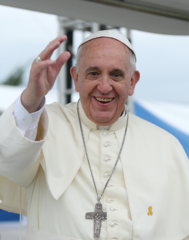
\includegraphics[scale=.5]{a20160315ShipofState-img001.png}
\end{minipage}~%
\begin{minipage}{.45\textwidth}
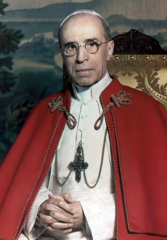
\includegraphics[scale=.5]{a20160315ShipofState-img002.png}
\end{minipage}
\caption{Pope Francis / Pope Pius XII}
\end{figure}

\hfill



\flrightit{Posted on 2016-03-15 by Cologero }

\begin{center}* * *\end{center}

\begin{footnotesize}\begin{sffamily}



\texttt{Cologero on 2016-03-18 at 12:29 said: }

Here are some examples of the use of lawlessness and chaos as a political tactic.

\textit{When the Law Is a Drag:} \url{https://pjmedia.com/victordavishanson/law-is-a-drag/?singlepage=true}

\textit{France's Highways Descend Into Chaos \& Lawlessness:} \url{http://www.zerohedge.com/news/2016-01-26/frances-highways-descend-chaos-lawlessness}


\hfill

\texttt{Sparrow on 2016-03-21 at 00:15 said: }

Coincidentally, I've recently been reading on Hegel's views of the spirit and physiognomy. Racial political correctness did not exist back in the day, but Hegel seems quite eager to correct himself. He asserts that ``spirit leaves nothing to chance," then in another work asserts that physical differences do not reflect the spirit and are ``accidents." of course, the physiognomy of Hegel's day was largely materialistic, he may have been more accepting to Evola's belief in spiritual races.


\hfill

\texttt{Olavsson on 2016-03-21 at 14:37 said: }

We could compare Julius Evola and Frithjof Schuon, two ``Traditionalists" with a widely different style. Video is even more useful than photographs, as we can study changing expressions, voice intonations, gestures etc in better detail.

Schuon:

\url{https://www.youtube.com/watch?v=F9T90GWfk40}

Evola:

\url{https://www.youtube.com/watch?v=QiCtdi5nCoA}

Note that both men are aging in these recordings, so we see them after they have matured as much as they were capable of.

Evola comes much more alive to you when watching him in this format, than when seeing a few old black-and-white photographs for which he had posed pretentiously. He's certainly got charisma. Every now and then he reveals something almost ``vampyric" in a romantic-draculian-aristocratic sense (which I suspect he would even have taken as a compliment). It is also easy to see that he still retains strong residues of attachment to the ego-self. Does he come across as `noble'. Definitely, but mainly in the cultural and human degree of appealing to a historical archetype, which is done deliberately and self-consciously. I accept Evola's own discernment that he was a kshatriya as far as this four-fold caste-categorization is concerned. The entire aura of Schuon, on the other hand, is very characteristic of the sagely type, which is `noble' (arya) in a higher octave altogether. He appears spiritual in a deeper, more essential and selfless sense. (Note that I'm here ignoring the various personal controversies and so on, which would be to stray from the context in question.) But both men, Schuon as much as Evola, were possibly too concerned with outer image, and even in the case of Schuon, this might be a sign of a sublimated vanity. The purest spiritual nobility is that of men who do not deliberately and self-consciously act or appear in a certain manner because they know this is what signals nobility or spirituality, but rather that of men who spontaneously be this way without any thought of the self or any desire thereof or self-interest, who are genuinely selfless before the Divine as well as before others, and thus let the Heavenly wu-wei flow through them unhindered.

For we whose foremost interest when it comes to these men is the validity of Traditional doctrines and truths, the question of their personal qualities aside from their intellectual ability to get these things straight (and none of them—especially not Evola—were entirely infallible or unbiased in this respect) is largely uninteresting. But in this context, when we're concerned with the personal dimension, it may hold some limited relevance. In the preface to the English edition of `Introduction to Magic' (page xiv), we see that Evola's ex-lover Sibilla Aleramo says of him: ``He is inhuman, an icy architect of acrobatic theories, vain, vicious, perverse…" To Evola's defense, it may be pointed out that she was hardly unbiased, and her experience was with the young `magical' incarnation of him.

It should always be remembered that ``not all that is gold will glitter" when we study these things. A man or woman of high spiritual stature, or nobility, may not necessarily give us that impression immediately based on more superficial factors, our prejudices, preconceptions and so on, as our eye—and our integral knowledge—is simply not sufficiently subtle to notice everything that transcends our own inner condition to a considerable extent, and which may be concealed from curious eyes. But these things are never impossible to see for those possessing the required knowledge, as they leave definite signs in the outer being: whether WE as individuals, given our own limitations, are able to consciously register it is quite another question. Also, as the Christ said according to the Gospel of Thomas, ``There is light within a person of light, and it shines on the whole world; if it does not shine, it is dark."

One thing I do notice these days is that the outright evil of many members of the modern `elites' is very clearly reflected—in fact often grossly visible—in their countenance, almost as if they were demonically possessed. Especially the eyes are usually very revealing in this respect, being the ``mirror of the soul". There are many, many examples one could refer to, but in these days, Hillary Clinton would be one appropriate case to mention. For those who have eyes to see, the agents of the dark-side may be quickly identified thus, and one may even derive from such observation an impression of the varying degrees of inner `demonization' (being the fall into the infra-human, as Guenon would say, almost as an inverted transcendence) that dominate different personalities. Here we are dealing not merely with cases of inept and incompetent, mediocre `plebeians' who have been able to ascend to the ranks of power because of the quantitative reign of `demotism'. but in fact with something far more sinister. We must realize that there are even highly ``intelligent" and cunning elitists who work under the sign of evil, who are more than what the official images and stories that are presented make us believe. Without being able to see into the depths of such figures, to see which principal forces (and intelligences) they are serving and are infiltrated by (``possessed" of) beyond/behind the official political and ideological facade of the most superficial interests and agendas, we will remain forever blind to what Evola termed ``the third dimension of history" in his commentaries on the ``occult war."

Some final words: For the highest norm of a noble inner as well as outer ``style", we can do no better than studying sages and masters, saints etc whose lives were wholeheartedly dedicated to a single-minded quest for Divine Truth. To the extent they are fully permeated by this path, and have integrated their insights fully, it will show. No person should be taken as an ideal embodiment of any kind unless they are truly holy. Then it will only be a matter of the ``blind leading the blind." But if we mimic them for the sake of our egos, instead of sacrificing ourselves fully to the Way, we will have missed the entire point.


\hfill

\texttt{Harun on 2016-03-22 at 04:44 said: }

I would also consider a few legends about people looking the same.

The state of the being of someone can influence his physical appearance.

For example is the count of St.Germain immortal or is he a succession of initiates that look very similar and also share memories?

Also, Guénon mentioned in a letter to De Giorgio that St.Pius of Petralcina looked very similar to a contemporary sufi sheyk.


\hfill

\texttt{Cologero on 2016-03-22 at 21:19 said: }

Although the saying goes ``never judge a book by its cover", people can't avoid it. Of course, any worthwhile physiognamy isn't interested just in physical attractiveness. Presumably Evola, growing up in Italy, would have been aware of the tradition of physiognamy described in the following links (not taught in RCIA classes AFAIK):

\textit{The Eyes and the Gaze:} \url{http://www.traditioninaction.org/Cultural/A018cpManualCivility6_Gaze.htm}

\textit{The Face Reveals the Heart of the Man:} \url{http://www.traditioninaction.org/religious/n001rpFaceRevealsMan.htm}

\textit{Four Ways to Discern a Man's Soul by His Appearance:} \url{http://www.traditioninaction.org/religious/n003rpLapide_Appearance_2.htm}

\textit{The Eyes Are the Mirror of the Soul: } \url{http://www.traditioninaction.org/religious/n002rpLapide_Appearance.htm}


\hfill

\texttt{Cologero on 2016-03-22 at 21:40 said: }

Many interesting points, Olavsson. I would just confirm that the ordinary person is quite unskilled in this science, otherwise con men and psychopaths, not to mention most politicians, would have no careers. I recall my time at voir dire for jury selection. The attorney asked each of us how could we tell if someone was lying. Most women asserted they ``could see it in their eyes". I'm sure that outside the courtroom, those very women would complain about all the lies that men had told them.

Vanity traditionally has been considered the most subtle vice, since it often follows great spiritual progress. It seems unavoidable for anyone who strives to be a public figure, since motives can easily be confounded.

As for Miss Aleramo, her reaction is likely due to Evola's transcendence of bourgeois values. In particular, women sometimes get upset when a man can't be manipulated sexually.


\hfill

\texttt{Boreas on 2016-03-23 at 08:28 said: }

Interesting points Olavsson regarding Evola and Schuon. I've come to think Evola as some sort of a LHP figure lately, and this `personal equation' that he himself talked alot could perhaps show out also in his facial expressions and gestures. In my opinion there was always something `luciferian' about Evola, and this would show up both in his actions, in his personal weltanschauung and even in his physical personality. He was more a ``soulful" personality than purely ``spiritual" as for example Guénon or Schuon.

This also reminds me of Guénon's view that the ``revolt of the Kshatriyas" was a `luciferian' phenomenon (he mentioned it in `Spiritual Authority and Temporal Power'. if I recall correctly).


\hfill

\texttt{Max on 2016-03-29 at 09:08 said: }

Most people have quite boring facial features and expressions. Evola has an idiosyncratic expression as one would expect. One can usually come into contact with interesting people by simply being on the look out for interesting and differentiated expression. The predominant emotional state of a person often shows in the face, and there are often many signs of negative emotion in various forms. 

When studying people in for example public transport, it is very unusual to see someone who seems to be inner motivated – most are being carried away by various stimuli and acts as if on auto-pilot. Nowadays it is very rare to see someone simply sitting straight up with a good posture, having a clear and awake gaze, not distracting himself with some gadget, slumbering, talking loudly and incoherently, or just plain mentally drifting. The other day I was on the commuter train and an elderly couple clearly on temporary visit sat down on the opposing seats, actively seeking my eyes and smiling, there was a sense of emphatic and polite understanding, like a refreshing flash from a world that does not exist anymore, it made me think of what we have lost.


\hfill

\texttt{Olavsson on 2016-04-02 at 15:16 said: }

@Alistair Fraser:

There is an idea in certain initiatic currents that a highly capable master may, under certain conditions, ``transmit" by his power a particular inner state into a qualified disciple, an awakening to a higher state inspired by that direct contact with one in whom the inner state is transcendent in relation to one's own. In other words, an act of spiritual grace using the master as an intermediary. This may be very distantly related to what you experienced with that woman, though on a far more ordinary level. Of course, I think it's quite normal to have at least a small awareness of how differently we may be affected by the contact with diverse human types. It is important to learn the art of analyzing the effect of these contacts from the viewpoint of spiritual priorities. For example, we can decide to ``ride the tiger" of Kali-yuga and hang out at decadent underground nightclubs in the cities and risk being affected by the negative influences at work in such places, or we can simply stay away and distance ourselves increasingly from the low spirit of the times, thus creating ideal conditions for the contemplative path. (Beata solitudo, sola beatitudo…) We've always got a choice.

The same goes for the insidious onslaught of subversive propaganda that you mention, by which we are ambushed from all directions nowadays. We must close our doors upon it to the exact extent this is possible given our circumstances. Regarding propaganda (mentioned in Cologero's post), I recently came across an intriguing satanic counter-initiate (founder of the Temple of Set) who used to work within US military with an above top secret security clearance, Dr. Michael Aquino; he has apparently written a book called `MindWar'. regarding which he says:

``There is no defense whatever against MW PSYCONs, because they access the subconscious, not the conscious thought process. You would have absolutely no idea a MW campaign was being directed against you unless you knew exactly what to look for, and quite possibly not even then."

But if we are firmly rooted in an orthodox Traditional worldview, metaphysics and esoterism, and are able to thoroughly and deeply apply the proper First Principles to everything, always remaining watchful and guarding our own minds, I cannot see how exactly the enemy would be able to influence us through the subconscious to the degree of conditioning our reactions and orientations in the world. There is a great difference between the average man in the street and, say, a Guénon. So why does our satanic Dr. Aquino want us to believe there is ``no defense whatever" against it? Curious, isn't it? Perhaps in order to subtly plant the sinister suggestion that certain elites are almighty, like God, and cannot possibly be opposed? Men like him, and so much the more when they have been involved in extensive scientific research into these matters, are masters of manipulation, and everything they say should be closely scrutinized, never taken at face value.

Re: the Evola video footage: It is true that this interview was filmed after his war accident, but his entire upper body was unaffected, so I don't think his facial expressions and so on would have been particularly changed. He seems pretty natural and effortless in that video. I would have paid more to see a video of Guenon than the younger Evola, as a matter of fact. Also, being more or less Hermetists, after all, we will know that this very significant and dramatic incident in the life of Evola symbolically corresponds to a facet of his inner condition. Evola himself—having a metaphysical and spiritual rather than profane/modern outlook on every aspect of reality—knew it wasn't a mere isolated coincidence, but he apparently never attained certainty as to the deeper reason for his fate. If my memory serves me right, Mircea Eliade also thought it signalled something about his inner condition. My own suggestion is that the answer to why it happened was hidden where Evola would have been the least interested in searching for it, as it would (perhaps) have humbled him more than a little. Anyhow, he faced these challenging last years of his life with admirable inner strength, and I hope that God granted him in death at least some of the liberation he had lived for. How interesting it would have been to be able to trace his (and others'. postmortem destiny.

@Cologero:

Seeing through lies is not so easy if one wants to believe the lies. One word: detachment. And what you say about vanity is the plain truth.

Re: Aleramo: You might be right about that. While I am as defiant towards the bourgeois way of life as anyone, simply because it is completely contrary to my nature, one should nevertheless be careful not to make this a guiding principle of its own, which may possibly even take precedence over more essential principles. What must ultimately be transcended is the lower self, after all, which is perfectly capable of reinforcing itself even while `transcending' bourgois norms.

@Boreas:

You are right to view Evola's own chosen course as basically ``LHP" (``Left-Hand Path), which I do not think he would have protested, based on various statements in the video interview I linked to, for example. Here we can mention his individualistic and independent approach to the path, not having made commitment to any formal tradition, but that is widespread in our age and doesn't necessarily make one LHP. However, his insistence on not answering to any spiritual authority higher than his own individual self, almost a `promethean' approach to transcendence (which is why the way of the magus initially appealed to him), his fascination with what he himself termed the ``antinomianism" of certain Hindu tantras (a tradition which Guénon, incidentally, thought Evola wasn't fit to deal with…), and his attempt to practice Left-Hand Tantrism as a `freelancer' outside a proper traditional context—all of this, and more, combine to make him quite LHP, if we define this term in the broadest fashion possible, allowing for many nuances. It is important to emphasize, however, that this does not at all mean he considered his own solution an ideal path to be emulated from a general point of view. (For example, he referred someone to Sufism, curiously saying that he himself was more interested in ``power" than spirituality.) Personally, I am prone to suggest that Evola placed spiritual limitations upon himself, ironically due to a quest for individual spiritual freedom, independence and self-sufficiency, that could have been overcome if he had submitted himself to a more regular path as was done by a Guénon.

As for Evola's ``personal equation", I think you are right in describing him as more of a ``soulful" than a ``purely spiritual" type, which is not so strange considering his kshatriya nature. He often spoke of the unconditioned Absolute, but due to this personality factor, I doubt that he would ever have been suited for anything above the ``Lesser Mysteries", which in any case is the initiatic domain that has typically been appropriate for kshatriyas according to Guénon. Esoterism in Europe seems seldom to have went beyond it.

And speaking of the ``revolt of the kshatriyas", it is interesting that Red is considered a stage superior to White in esoteric alchemy, which (as Evola never tired of pointing out) identifies itself much with royal symbolism—almost as if the Will is above Intellection, or the Soul above the Spirit. This is a theme that keeps returning in deviated initiations. (Well exemplified by Crowley's famous maxim, ``Do what thou wilt shall be the whole of the law", as if the Great Quest can start and end with the isolated self-will of some individuated ``I" that is, moreover, in a fallen state).

Also, there are several things that could be mentioned in connection to the ``revolt of the kshatriyas", Luciferianism and the Counter-Initiation, all of which may be inter-related, but it will have to wait, for this comment is getting too lengthy.


\hfill

\texttt{Tom on 2016-04-07 at 05:47 said: }

There are examples in Indo-European traditions of Physiognomy besides the obvious caste distinctions of Hinduism. In Old Norse literature we can see clearly from Rígsthula that the three castes could be identified by physical characteristics with the lowest being the darkest. More subtle examples can be found in the sagas where physical attributes have cultural and symbolic significance in. They reveal aspects of a person's character, disposition and their future. Very often the symbolic nature of a character is identified by their lineage and their behaviour, but both of these variables can in turn be related to the physical attributes of that character. In Njals saga, Hrútr describes his niece Hallgerdhr as having ``thieves' eyes", which is a portent to the coming events of the novel generated by Hallgerdhr's un womanly and dominating nature. later in the saga Hallgerdhr makes scathing comments about the appearances of Bergthóra, Njáll, and their sons (whom she calls dung-beardlings due to the implied shame of the fact their father Njall is unable to grow a proper beard); this physical lack is a signifier of implied sexual inadequacy. All this contrasts greatly with the physical description in the same saga of the heroic character Gunnar:

``He was handsome and fair of skin and had a straight nose, turned up at its tip. He was blue-eyed and keen eyed and ruddy cheeked, with thick hair, blonde and well combed."


\hfill

\texttt{Thomas Blanchard on 2016-07-11 at 16:49 said: }

I was reminded of this post while reading Plinio Corrêa de Oliveira's physiognomic analysis of political revolutionaries' faces, which I'll share here as it may be of some interest: \url{http://nobility.org/2016/02/18/three-faces-of-the-revolution/}

As children, it feels natural to make inferences about character based on physical appearance (and particularly facial features), although most modern adults suppress these judgements as they're taught not to.


\hfill

\texttt{Max on 2016-09-11 at 14:56 said: }

Here is a passage from George Duby's book on medieval artwork ``The Age of the Cathedrals" under the heading of ``Faces":

``The growing number of characters in the liturgical drama filling the theaters in the cathedral porches meant that each had to be distinguished. Certainly they bore their insignia, the special attribute given to each prophet, each precursor, each apostle in Christian iconography, but they also had to be endowed with personal features capable of conveying a specific psychological expression. The vocabulary of the literary works available to knights in the thirteenth century was extremely poor. Joinville abounded in eloquent portrayals of spirited combat and the motley glamor of courtly gatherings, but became tongue-tied when it was a matter of describing character. In practical life at any rate, in the surveys carried out to ascertain the distribution of feudal rights or to settle points of usage and sometimes even before their confessors, the lords, great and small, gradually sharpened their analytical ability. As for the academic world, it was accustomed to introspection, which already offered a foothold for the morality of Abelard. All theology led to ethics. It involved the exploration of the soul, the classification of its capacities and its virtues. And as the intellectual system of doctors was based on the principle of the unity of the universe, as it asserted the close cohesion of the three components of the human being – mind, soul, and body – it naturally considered that facial features faithfully translated individual dispositions. The scholastic approach, however, was bent on resolving the particularities of each individual through the forms common to his species. It proceeded by distinguishing kinds. More exactly, then, the faces of the statues represent types of men."

The practical science of Physiognomy then, seems primarily to have been a domain of artisans and knights rather than schoolmen, which contributes to its perception as a Hermetic discipline, for in the old tales we find the wise hermit as a retired knight. The intellectual class can be prone to too much abstraction when focusing at what is common to the species, which we need to remember is nevertheless made up of individuals with distinguishing marks. The usage of ``species" seems to have undergone quite a lot of change throughout history and should refer more to what is ``seen" as a ``medium of knowledge" than a dry external classification. \url{http://www.newadvent.org/cathen/14210a.htm}

On the topic of seeing I found the man in this photo an interesting study, perhaps with a tangent to Swedenborg's claims on hidden teachings, which is unlikely to refer to physical writings in any case: \url{http://frontierphotos.blogspot.se/2008/11/bonpo-lama-from-radja-gomba.html}

Primary importance is given to the subtle expression rather than hard facial features, even though those matter as well. This poses a difficulty for art and sculpture since it is naturally easier to capture the outward form than the formless aspect of a person. However, in the ancient world they would also ritually ``animate" statues so as to not merely see it as a lump of rock. 

The species cannot, in the manner of enlightenment rationalism, be isolated from the spectrum that ties the intellectual to the corporeal. We can take the term ``specter" as referring to particular visions of the intermediary realm, however it is curiously enough also an anagram of ``scepter", the insignia of the emperor signifying temporal authority and power, raising images not only of the legitimate ruler but of the specter of the earth, ideas which seems to be somehow connected. To some degree, a ruler will at least need an understanding if not mastery over appearances and the interplay of soft and hard.

``To establish the Way of Heaven: that is yin plus yang. To establish the Way of Earth: that is soft [jou] plus hard [yo]. To establish the Way of Man: that is humanity plus justice" – I Ching, as quoted by Guenon


\end{sffamily}\end{footnotesize}

\section{Independence Day}

\begin{quotex}
Man is neither the slave of his race nor his language, neither of his religion nor of the course of rivers, not yet of the direction of mountain ranges. A great aggregation of men, healthy in mind and warm in heart, creates that moral consciousness that we call a nation. As long as this moral consciousness proves its strength by the sacrifices that are required by the abdication of the individual to the benefit of a community, it is legitimate and has the right to exist. \flright{\textsc{Ernest Renan}, \textit{What is a Nation} (1882)}

\end{quotex}
\paragraph{The Liberal State}
Renan expresses the liberal position of the 19th century: a nation is the result of Will, not Destiny (natural or familial relationships), certainly not Providence (divine sanction). Every July 4, the USA celebrates its independence day as the first liberal state. It is to nations as Esperanto is to languages. It is instructive to compare its founding to that of traditional societies.

The \textbf{Declaration of Independence} expressed the fundamental principle that governments derive their just powers from the consent of the governed. This is the opposite of the traditional view that temporal power is derived from spiritual authority, or the consent of God or the gods. This gave them remarkable stability and they typically endured for a long time. Of course, that really meant that they were really based on a transcendental principle. But the masses are fickle. As Renan explains:

\begin{quotex}
We have expelled metaphysical and theological abstractions [i.e., any transcendent principle] from politics. What remains after this? There remains man, his desires and his needs.

\end{quotex}


A man's desire is insatiable and his needs vary with circumstances; hence the liberal state will always be subject to such vagaries. Since desires are infinite and resources finite, the liberal state will always experience internal conflicts and its primary task is to arbitrate competing interests. As long as resources are sufficient, stability can be maintained.

Nevertheless, stability is not stasis and power blocs will always try to grab more. This is actually enshrined in the Declaration: In response to a ``long train of abuses and usurpations", the \emph{governed have the right and duty to throw off such government}. That is why political discourse is so often framed in terms of abuses and injustices; that justifies all attempts to radically alter the mores and laws of the country. Pathetic appeals by so-called conservatives to the ``original intent" of the Constitution, therefore, are quite beside the point.

The other useless tactic of conservatives is to argue in terms of transcendent principles, which are irrelevant in a system whose only criteria are the passing whims of the governed. If everyone is equal, then there is no hierarchy. If there is no hierarchy, there is denial of divine order. That is why revolutions are always atheistic, both the French and the Bolshevik. The masses profess atheism, at least materially if not formally. This is the insight of \textbf{Valentin Tomberg}.

\paragraph{Theocracy and Republic}
In his \textit{Hermeneutic Interpretation of the Origin of the Social State of Man}, published in 1822, \textbf{Fabre d'Olivet} provides a panoramic history of the human race, not in terms of facts, but in terms of the inner forces behind the events. Greece and Rome were theocracies under the reign of a priest-king before they became republics as we pointed out.\footnote{\url{https://gornahoor.net/?p=2554}} Yet, they still retained the idea of divine sanction. Plato said in the Laws that is was necessary to consult first the oracle of Delphi. All of the republics of ancient Greece invoked the Divinity at their inception. Rome had a sovereign pontiff (chief priest), although his influence gradually waned. Fabre makes some interesting points about the USA, less than 50 years after its Constitution.

The USA were ``the fruits of a political schism whose principal aim has been to destroy sacerdotal authority. No sovereign pontiff exists in the United States and cannot exist there." He then makes a telling point that nearly 200 years later, conservatives still have not grasped:

\begin{quotex}
By quite a strange inversion, it is possible in this republic that all the citizens are religious without the government having the least religion; that they are all pious, even devout, virtuous, scrupulously upright, without the government having the least piety, the least devotion, the least virtue, the least probity. For the government is a purely political being which adopts the sentiments of none of its members, and which above all in point of religion, affects an absolute indifference.

Now, as this government has above it no spiritual power to which it owes account of its conduct, and that even God does not exist for it [that is, the idea of God is never part of its political acts], although it may exist in different ways for each of its members, it follows from this that it is really without religion in its political constitution and that the law which constitutes it and which emanates from it is atheistic. 

\end{quotex}
This is why conservatives are so muddle headed. They repeatedly point to the religious beliefs of the nation's founders as though they are of significance. The state itself is atheist; as long as the governed, who give it their consent, adhere to a specific creed, no one may notice it. Hence, as the demographic makeup of the population is altered, its whims change and it gives consent to other laws. New power blocs arise each claiming abuses (injustices) and usurpations (unequal sharing of goods), which requires a continual overthrow of the government (hope and change). Conservatives claim foul, when long held moral beliefs are suddenly overthrown. Yet, that is no more than the system behaving as designed.

So it is not Christianity that leads to democracy, liberalism, socialism and egalitarianism as some political commentators of the New Right insist, but rather the atheist state as exemplified in America, France and Soviet Union.



\flrightit{Posted on 2011-07-03 by Cologero }

\begin{center}* * *\end{center}

\begin{footnotesize}\begin{sffamily}



\texttt{James O'Meara on 2011-07-05 at 11:09 said: }

I would recommend James Kalb's The Tyranny of Liberalism for a quasi-Traditionalist [really, neo-Catholic] account of the phony `tolerance' of Liberalism, especially in terms of seeking a phony ``objective" balancing of mere desires.

Americans are so brainwashed by their ``civics" and ``history" classes [if, that is, they remember anything at all] and so ignorant of the rest of the world, that they continue to ``think" that the USA is ``the greatest country on Earth" and ``the envy of everyone else". Why 9/11, for example? ``They hate us for our freedom." I was much amused when Bin Laden himself gave the response I had given for years: ``Then why didn't I attack Sweden?"

Speaking of Sweden, Americans never notice that after almost 300 years not one nation has adopted their absurd and ineffective system of ``check and balances" etc. Not even when the USA imposes a constitution on them [post war Japan or Iraq, for example]. For the rest of the world, `democracy' means parliamentary democracy, a la the superior British system, not the crude cargo-cult version cobbled together by men who, as Jefferson admitted, went into politics because there was nothing else to do in this god-forsaken wilderness.

More to your point, though: the unique features of the American system are entirely religious. Concern with ``founding fathers" [Patriarchs], a constitution written [unlike England] and unlike other written constitutions not subject to more than trivial alteration by the voters [contrary to your presentation, which is more applicable to France or Sweden, say] but rather treated as a Sacred Scripture to be ``interpreted" by a sanctified group of priests in black robes searching out ``original intent" — what is this?

This is certainly Protestantism, and back of that, of course, Judaism, Protestantism representing the resurgence of `primitive Christianity' against the Roman tradition.

It is interesting to note that this Protestant institution, the Supreme Court, now has not one Protestant on it, divided equally between Jews and Catholics. Jews, obviously, and as for the ``Catholics," their leader, Justice Scalia's quoting the Talmud and working to found an Academy of Talmudic Law show where his loyalty lies.

Tradition, of course, is not the source of Liberalism etc. [see the Syllabus of Errors] but once the unity of Church and Empire was broken,the result was Protestantism, the secular state, Liberalism, socialism, etc., back of all of which is the `primitive Christianity' that had been held in check by the ``Roman" part of the Roman Church.

That current Liberalism seems to be increasingly ``officially" atheist [Hitchens, etc.] is irrelevant. Each stage advances, leaving some behind [just as you say, new groups are added to the mix]; 18th century Protestants bemoan the ``social gospel" types, they bemoan the agnostics, they bemoan the atheists, etc. Where, what's the next stage? Only the final abyss of the Kali Yuga.


\hfill

\texttt{Cologero on 2011-07-07 at 07:47 said: }

All good points except for: ``not subject to more than trivial alteration by the voters [contrary to your presentation"

Of course, since that claim is never made in the ``presentation". But the ``consent of the governed" is found in the idea of the ``living constitution" rather than the fundamentalist analog of the ``original intent". So no one bothers with the ``word" anymore. Over the past 60 years or so, decisions by the federal courts, sweeping and vague laws from congress, and the rule of the executive by rules and regulations of federal agencies have resulted in far from trivial changes in actual life.


\hfill


\end{sffamily}\end{footnotesize}


\end{document}
